\documentclass[12pt]{book}

\title{Think Java}
\author{Allen B. Downey and Chris Mayfield}

\newcommand{\thetitle}{Think Java}
\newcommand{\thesubtitle}{How to Think Like a Computer Scientist}
\newcommand{\theauthors}{Allen B. Downey and Chris Mayfield}
\newcommand{\theversion}{6.5.0}

%%%% Both LATEX and PLASTEX

\usepackage{graphicx}
\usepackage{setspace}

%BEGIN LATEX
\usepackage{comment}
\excludecomment{htmlonly}
\includecomment{latexonly}

\usepackage{imakeidx}
\makeindex[options= -s headings.ist]
%END LATEX

% automatically index glossary terms
\newcommand{\term}[1]{%
\item[#1:]\index{#1}}

\usepackage{amsmath}
\usepackage{amsthm}

% format end of chapter excercises
\newtheoremstyle{exercise}
  {12pt}        % space above
  {12pt}        % space below
  {}            % body font
  {}            % indent amount
  {\bfseries}   % head font
  {}            % punctuation
  {12pt}        % head space
  {}            % custom head
\theoremstyle{exercise}
\newtheorem{exercise}{Exercise}[chapter]

\newif\ifplastex
\plastexfalse

%%%% PLASTEX ONLY
\ifplastex

\usepackage{localdef}

\usepackage{url}

\newcount\anchorcnt
\newcommand*{\Anchor}[1]{%
  \@bsphack%
    \Hy@GlobalStepCount\anchorcnt%
    \edef\@currentHref{anchor.\the\anchorcnt}%
    \Hy@raisedlink{\hyper@anchorstart{\@currentHref}\hyper@anchorend}%
    \M@gettitle{}\label{#1}%
    \@esphack%
}

% code listing environments:
% we don't need these for plastex because they get replaced
% by preprocess.py
%\newenvironment{code}{\begin{verbatim}}{\end{verbatim}}
%\newenvironment{stdout}{\begin{verbatim}}{\end{verbatim}}

% inline syntax formatting
\newcommand{\java}{\verb}%}

%%%% LATEX ONLY
\else

\usepackage{geometry}
\geometry{
    width=5.5in,
    height=8.5in,
    hmarginratio=3:2,
    vmarginratio=1:1,
    includehead=true,
    headheight=15pt
}

% paragraph spacing
\setlength{\parindent}{0pt}                      % 17.62482pt
\setlength{\parskip}{12pt plus 4pt minus 4pt}    % 0.0pt plus 1.0pt
\linespread{1.05}
\def\arraystretch{1.5}

% list spacing
\setlength{\topsep}{5pt plus 2pt minus 3pt}      % 10.0pt plus 4.0pt minus 6.0pt
\setlength{\partopsep}{-6pt plus 2pt minus 2pt}  %  3.0pt plus 2.0pt minus 2.0pt
\setlength{\itemsep}{0pt}                        %  5.0pt plus 2.5pt minus 1.0pt

% these are copied from tex/latex/base/book.cls
% all I changed is afterskip
\makeatletter
\renewcommand{\section}{\@startsection{section}{1}{\z@}%
    {-3.5ex \@plus -1ex \@minus -.2ex}%
    {0.7ex \@plus.2ex}%
    {\normalfont\Large\bfseries}}
\renewcommand\subsection{\@startsection{subsection}{2}{\z@}%
    {-3.25ex\@plus -1ex \@minus -.2ex}%
    {0.3ex \@plus .2ex}%
    {\normalfont\large\bfseries}}
\renewcommand\subsubsection{\@startsection{subsubsection}{3}{\z@}%
    {-3.25ex\@plus -1ex \@minus -.2ex}%
    {0.3ex \@plus .2ex}%
    {\normalfont\normalsize\bfseries}}
\makeatother

% table of contents vertical spacing
\usepackage{tocloft}
\setlength\cftparskip{8pt plus 4pt minus 4pt}

% balanced index with TOC entry
\usepackage[totoc]{idxlayout}

% The following line adds a little extra space to the column
% in which the Section numbers appear in the table of contents
\makeatletter
\renewcommand{\l@section}{\@dottedtocline{1}{1.5em}{3.0em}}
\makeatother

% customize page headers
\usepackage{fancyhdr}
\pagestyle{fancyplain}
\renewcommand{\chaptermark}[1]{\markboth{Chapter \thechapter ~~ #1}{}}
\renewcommand{\sectionmark}[1]{\markright{\thesection ~~ #1}}
\lhead[\fancyplain{}{\bfseries\thepage}]%
      {\fancyplain{}{\bfseries\rightmark}}
\rhead[\fancyplain{}{\bfseries\leftmark}]%
      {\fancyplain{}{\bfseries\thepage}}
\cfoot{}
%\usepackage[mmddyyyy]{datetime}
%\rfoot{\textcolor{gray}{\tiny \thetitle, \theversion, \today}}

%% tweak spacing of figures and captions
%\usepackage{floatrow}
%\usepackage{caption}
%\captionsetup{
%    font=small,
%    labelformat=empty,
%    justification=centering,
%    skip=4pt
%}

% colors for code listings and output
\usepackage{xcolor}
\definecolor{bgcolor}{HTML}{FAFAFA}
\definecolor{comment}{HTML}{007C00}
\definecolor{keyword}{HTML}{0000FF}
\definecolor{strings}{HTML}{B20000}

% syntax highlighting in code listings
\usepackage{textcomp}
\usepackage{listings}
\lstset{
    language=java,
    basicstyle=\ttfamily,
    backgroundcolor=\color{bgcolor},
    commentstyle=\color{comment},
    keywordstyle=\color{keyword},
    stringstyle=\color{strings},
    columns=fullflexible,
    emph={label},  % keyword?
    keepspaces=true,
    showstringspaces=false,
    upquote=true,
    xleftmargin=15pt,  % \parindent
    framexleftmargin=3pt,
    aboveskip=\parskip,
    belowskip=\parskip
}

% code listing environments
\lstnewenvironment{code}
{\minipage{\linewidth}}
{\endminipage}
\lstnewenvironment{stdout}
{\lstset{commentstyle=,keywordstyle=,stringstyle=}\minipage{\linewidth}}
{\endminipage}

% interactive code listing
\lstnewenvironment{trinket}[2][400]
{\minipage{\linewidth}}
{\endminipage}

% inline syntax formatting
\newcommand{\java}[1]{\lstinline{#1}}%{

% prevent hyphens in names
\hyphenation{DrJava}
\hyphenation{GitHub}
\hyphenation{Javadoc}

% pdf hyperlinks, table of contents, and document properties
\usepackage{hyperref}
\hypersetup{%
  pdftitle={\thetitle: \thesubtitle},
  pdfauthor={\theauthors},
  pdfsubject={Version \theversion},
  pdfkeywords={},
  bookmarksopen=false,
  bookmarksnumbered=true,
  colorlinks=true,
  citecolor=black,
  filecolor=black,
  linkcolor=black,
  urlcolor=blue
}

% add dot after numbers in pdf bookmarks
\makeatletter
\renewcommand{\Hy@numberline}[1]{#1. }
\makeatother


\fi

%%%% END OF PREAMBLE
\begin{document}

\frontmatter

%%%% PLASTEX ONLY
\ifplastex

\maketitle

%%%% LATEX ONLY
\else

\begin{latexonly}

%--half title-------------------------------------------------
\thispagestyle{empty}

\begin{flushright}
\vspace*{2.0in}

\begin{spacing}{3}
{\huge \thetitle} \\
{\Large \thesubtitle}
\end{spacing}

\vspace{0.25in}

Version \theversion

\vfill
\end{flushright}

%--verso------------------------------------------------------
\newpage
\thispagestyle{empty}

\quad

%--title page-------------------------------------------------
\newpage
\thispagestyle{empty}

\begin{flushright}
\vspace*{2.0in}

\begin{spacing}{3}
{\huge \thetitle} \\
{\Large \thesubtitle}
\end{spacing}

\vspace{0.25in}

Version \theversion

\vspace{1in}

{\Large \theauthors}

\vspace{0.5in}

{\Large Green Tea Press}

{\small Needham, Massachusetts}

\vfill
\end{flushright}

%--copyright--------------------------------------------------
\newpage
\thispagestyle{empty}

Copyright \copyright ~2017 \theauthors.

\vspace{0.2in}

\begin{flushleft}
Green Tea Press \\
9 Washburn Ave \\
Needham, MA 02492
\end{flushleft}

Permission is granted to copy, distribute, and/or modify this work under the terms of the Creative Commons Attribution-NonCommercial-ShareAlike 4.0 International License, which is available at \url{https://creativecommons.org/licenses/by-nc-sa/4.0/}.

The original form of this book is \LaTeX\ source code.
Compiling this code has the effect of generating a device-independent representation of the book, which can be converted to other formats and printed.

The \LaTeX\ source for this book is available from \url{http://thinkjava.org/} and \url{https://github.com/ChrisMayfield/ThinkJava2}.

%--table of contents------------------------------------------

\cleardoublepage
\setcounter{tocdepth}{1}
\tableofcontents

\end{latexonly}

%--HTML title page--------------------------------------------

\begin{htmlonly}

\vspace{1em}

{\Large \thetitle: \thesubtitle}

{\large \theauthors}

Version \theversion

\vspace{1em}

Copyright \copyright ~2017 \theauthors.

Permission is granted to copy, distribute, and/or modify this work under the terms of the Creative Commons Attribution-NonCommercial-ShareAlike 4.0 International License, which is available at \url{https://creativecommons.org/licenses/by-nc-sa/4.0/}.

\vspace{1em}

\end{htmlonly}

%-------------------------------------------------------------

% END OF THE PART WE SKIP FOR PLASTEX
\fi

\chapter*{Preface}

\markboth{PREFACE}{PREFACE}
\addcontentsline{toc}{chapter}{Preface}

{\it Think Java} is an introduction to computer science and programming intended for readers with little or no experience.
We start with the most basic concepts and are careful to define all terms when they are first used.
The book presents each new idea in a logical progression.
Larger topics, like control flow statements and object-oriented programming, are divided into smaller examples and introduced over the course of several chapters.

This book is intentionally concise.
Each chapter is 12--14 pages and covers the material for one week of a college course.
It is not meant to be a comprehensive presentation of Java, but rather, an initial exposure to programming constructs and techniques.
We begin with small problems and basic algorithms and work up to object-oriented design.
In the vocabulary of computer science pedagogy, this book uses the ``objects late'' approach.


\section*{The philosophy behind the book}

Here are the guiding principles that make the book the way it is:

\begin{itemize}

\item {\em One concept at a time.}
We break down topics that give beginners trouble into a series of small steps, so that they can exercise each new concept in isolation before continuing.

\item {\em Balance of Java and concepts.}
The book is not primarily about Java; it uses code examples to demonstrate computer science.
Most chapters start with language features and end with concepts.

\item {\em Conciseness.}
An important goal of the book is to be small enough so that students can read and understand the entire text in a one-semester college or AP course.
%Students can read 1--2 chapters per week, depending on the pace of the instruction.

\item {\em Emphasis on vocabulary.}
We try to introduce the minimum number of terms and define them carefully when they are first used.
We also organize them in glossaries at the end of each chapter.

\item {\em Program development.}
There are many strategies for writing programs, including bottom-up, top-down, and others.
We demonstrate multiple program development techniques, allowing readers to choose methods that work best for them.

\item {\em Multiple learning curves.}
To write a program, you have to understand the algorithm, know the programming language, and be able to debug errors.
We discuss these and other aspects throughout the book, and include an appendix that summarizes our advice.

%\item {\em Spiral approach.}
%Some concepts take time to sink in.
%The more difficult ideas in the book, like recursion, appear several times.
%By coming back to these topics, we give learners a chance to review and reinforce.

%\item {\em Keep it simple.}
%We use the minimum amount of Java to get the maximum amount of programming ability.
%The goal of this book is to teach fundamental ideas from computer science, not Java.
%We leave out some language features, like the \java{switch} statement, that are unnecessary, and we present only a few of the many classes in the Java libraries.

\end{itemize}


\section*{Object-oriented programming}

Some Java books introduce classes and objects immediately; others begin with procedural programming and transition to object-oriented more gradually.

Many of Java's object-oriented features are motivated by problems with previous languages, and their implementations are influenced by this history.
Some of these features are hard to explain when people aren't familiar with the problems they solve.

We get to object-oriented programming as quickly as possible (beginning with Chapter~\ref{immutable}).
But we introduce concepts one at a time, as clearly as possible, in a way that allows readers to practice each idea in isolation before moving on.
So it takes some time to get there.

You can't write Java programs (even hello world) without encountering object-oriented features.
In some cases we explain a feature briefly when it first appears, and then explain it more deeply later on.

This book is well suited to prepare students for the AP Computer Science A exam, which includes object-oriented design and implementation.
(AP is a registered trademark of the College Board.)
We introduce nearly every topic in the ``AP Java subset'' with a few exceptions.
A mapping of {\it Think Java} section numbers to the current AP course description is available on our website: \url{http://thinkjava.org/}.


\section*{Changes to the 2nd edition}

This new edition is three years in the making, with feedback from dozens of instructors and hundreds of students.
A complete history of all changes is available on GitHub.
Here are some of the highlights:

\begin{description}

\item[Chapters 1--4:]

We reordered the material in Chapter~1 to present a more interesting balance of theory and practice.
Chapters 2--3 are much cleaner now too.
The material on if statements and logic operators has been moved to Chapter 4, along with additional in-depth examples.

\item[Chapters 5--8:]

These chapters received the most attention.
We rearranged the content, added many examples and new figures, and removed unnecessary details.
Methods are now presented in a single chapter, and strings are covered earlier (before arrays) so that readers can apply them to loop problems.
The material on recursion is now a chapter, and we added new sections to explain binary numbers and CodingBat problems.

\item[Chapters 9--12:]

Our main goal for these chapters was to provide better explanations and more diagrams.
Chapters~9 and 10 focus more on immutable vs mutable objects, and we added new sections on BigInteger and StringBuilder.
The other content is largely the same, but it should be easier to understand now.

\item[Chapters 13--16:]

We balanced the amount of content in Chapters~13--14 by moving ArrayLists earlier, and we implement the ``War'' card game as another example.
Chapters~15--16 are brand new in this edition, and they cover more advanced topics including interfaces, polymorphism, and multi-dimensional arrays.

\item[Appendixes:]

We added Appendix~\ref{javadoc} to explain documentation comments and Javadoc in more detail.
%Most of the examples in the chapters do not include documentation comments to save space.
The other three appendixes that were present in the first edition have been revised for clarity and layout.

\end{description}


\section*{About the appendixes}

The chapters of this book are meant to be read in order, because each one builds on the previous one.
We also include several appendixes with material that can be read at any time:

\begin{description}

\item{\bf Appendix A: Tools}

This appendix explains how to download and install Java so you can compile programs on your computer.
It also provides a brief introduction to DrJava -- an ``integrated development environment'' (IDE) that is designed primarily for students -- and other development tools, including Checkstyle for code quality and JUnit for testing.

\item{\bf Appendix B: Javadoc}

It's important to document your classes and methods so that other programmers (including yourself in the future) will know how to use them.
This appendix explains how to read documentation, how to write documentation, and how to use the Javadoc tool.

\item{\bf Appendix C: Graphics}

Java provides libraries for working with graphics and animation, and these topics can be engaging for students.
The libraries require object-oriented features that students will not completely understand until after Chapter~\ref{mutable}, but they can be used much earlier.

\item{\bf Appendix D: Debugging}

We provide debugging suggestions throughout the book, but we also have an appendix with many more suggestions on how to debug your programs.
We recommend that readers review this appendix frequently as they work through the book.

\item{\bf Appendix E: Extras}

With each new edition, we add new material, remove old material, and revise everything else.
Some of the old material may still be useful, so rather than delete it, we moved it to this appendix.

\end{description}


\section*{Using the code examples}
\label{code}

Most of the code examples in this book are available from a Git repository at \url{https://github.com/ChrisMayfield/ThinkJavaCode2}.
Git is a ``version control system'' that allows you to keep track of the files that make up a project.
A collection of files under Git's control is called a ``repository''.

\index{repository}
\index{GitHub}

GitHub is a hosting service that provides storage for Git repositories and a convenient web interface.
It provides several ways to work with the code:

\begin{itemize}

\item You can create a copy of the repository on GitHub by pressing the {\sf Fork} button.
If you don't already have a GitHub account, you'll need to create one.
After forking, you'll have your own repository on GitHub that you can use to keep track of code you write.
Then you can ``clone'' the repository, which downloads a copy of the files to your computer.

\item Alternatively, you could clone the original repository without forking.
If you choose this option, you don't need a GitHub account, but you won't be able to save your changes on GitHub.

\item If you don't want to use Git at all, you can download the code in a ZIP archive using the {\sf Download ZIP} button on the GitHub page, or this link: \url{http://tinyurl.com/ThinkJavaCode2}.

\end{itemize}

After you clone the repository or unzip the ZIP file, you should have a directory named {\tt ThinkJavaCode2} with a subdirectory for each chapter in the book.

All examples in this book were developed and tested using Java SE Development Kit 8.
If you are using a more recent version, the examples in this book should still work.
If you are using an older version, some of them may not.


\section*{Contributors over the years}

Many people have sent corrections and suggestions, and we appreciate their valuable feedback!
This list begins with Version 4.0 of the open-source edition, so it omits those who contributed to earlier versions.

\begin{itemize}

\item Ellen Hildreth used this book to teach Data Structures at Wellesley College and submitted a whole stack of corrections, along with some great suggestions.

\item Tania Passfield pointed out that some glossaries had leftover terms that no longer appeared in the text.

\item Elizabeth Wiethoff noticed that the series expansion of $\exp(-x^2)$ was wrong.
She has also worked on a Ruby version of the book.

\item Matt Crawford sent in a whole patch file full of corrections.

\item Chi-Yu Li pointed out a typo and an error in one of the code examples.

\item Doan Thanh Nam corrected an example.

\item Muhammad Saied translated the book into Arabic, and found several errors in the process.

\item Marius Margowski found an inconsistency in a code example.

\item Leslie Klein discovered another error in the series expansion of $\exp(-x^2)$, identified typos in the card array figures, and gave helpful suggestions to clarify several exercises.

\item Micah Lindstrom reported half a dozen typos and sent corrections.

\item James Riely ported the textbook source from LaTeX to Sphinx.
\\ \url{http://fpl.cs.depaul.edu/jriely/thinkapjava/}

\item Peter Knaggs ported the book to C\#.
\\ \url{http://www.rigwit.co.uk/think/sharp/}

\item Heidi Gentry-Kolen recorded several video lectures that follow the book.
\\ \url{https://www.youtube.com/user/digipipeline}

\item Waldo Ribeiro submitted a pull request that corrected a dozen typos.
\end{itemize}

We are especially grateful to the technical reviewers of the O'Reilly Media first edition: Blythe Samuels, David Wisneski, and Stephen Rose.
They found errors, made many great suggestions, and helped make the book much better.

Many students have given exceptional feedback, including Ian Staton, Tanner Wernecke, Jacob Green, Rasha Abuhantash, Nick Duncan, Kylie Davidson, Shirley Jiang, and Elena Trafton.

Other contributors who found one or more typos: Stijn Debrouwere, Guy Driesen, Andai Velican, Chris Kuszmaul, Daniel Kurikesu, Josh Donath, Rens Findhammer, Elisa Abedrapo, Yousef BaAfif, Bruce Hill, Matt Underwood, Isaac Sultan, Dan Rice, Robert Beard, Daniel Pierce, Michael Giftthaler, Chris Fox, Min Zeng, and Markus Geuss.

%\medskip

If you have additional comments or ideas about the text, please send them to: \href{mailto:feedback@greenteapress.com}{\tt feedback@greenteapress.com}.

Allen Downey and Chris Mayfield


\mainmatter

\chapter{Computer programming}
\label{theway}

The goal of this book is to teach you to think like a computer scientist.
This way of thinking combines some of the best features of mathematics, engineering, and natural science.
Like mathematicians, computer scientists use formal languages to denote ideas, specifically computations.
Like engineers, they design things, assembling components into systems and evaluating trade-offs among alternatives.
And like scientists, they observe the behavior of complex systems, form hypotheses, and test predictions.

\index{problem solving}

An important skill for a computer scientist is {\bf problem solving}.
It involves the ability to formulate problems, think creatively about solutions, and express solutions clearly and accurately.
As it turns out, the process of learning to program computers is an excellent opportunity to develop problem-solving skills.
%That's why this chapter is called, ``The way of the program''.
On one level you will be learning to write Java programs, a useful skill by itself.
But on another level you will use programming as a means to an end.
As we go along, that end will become clearer.


\section{What is a computer?}

Usually when people hear the word computer, they think of a desktop or laptop.
Not surprisingly, searching for ``computer'' on \href{https://images.google.com/}{\tt images.google.com} displays rows and rows of these types of machines.
However, in a more general sense, a computer can be any type of device that stores and processes data.

\href{http://www.dictionary.com/browse/computer}{\tt Dictionary.com} defines a computer as ``a programmable electronic device designed to accept data, perform prescribed mathematical and logical operations at high speed, and display the results of these operations.
Mainframes, desktop and laptop computers, tablets, and smartphones are some of the different types of computers.''

\index{hardware}
\index{processor}
\index{memory}
\index{CPU}
\index{RAM}

Each type of computer has its own unique design, but internally they all share the same type of {\bf hardware}.
The two most important hardware components are {\bf processors} (or CPUs) that perform simple calculations and {\bf memory} (or RAM) that temporarily stores information.
Figure~\ref{fig.cpuram} shows what these components look like.

\begin{figure}[!ht]
\begin{center}
%https://commons.wikimedia.org/wiki/File:Intel_80486DX2_top.jpg
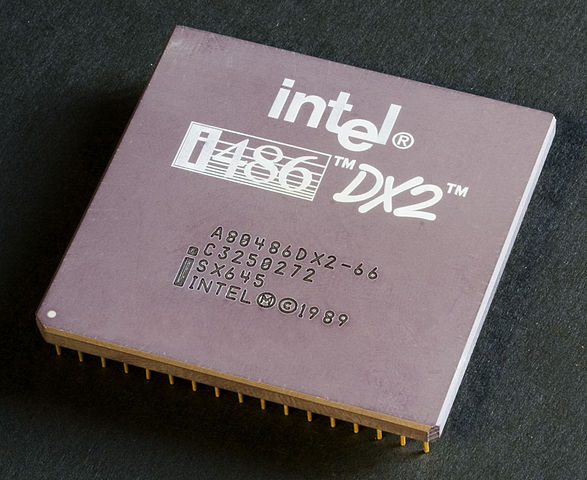
\includegraphics[height=11em]{figs/CPU.jpg}
\hspace{2em}
%https://commons.wikimedia.org/wiki/File:Memory_module_DDRAM_20-03-2006.jpg
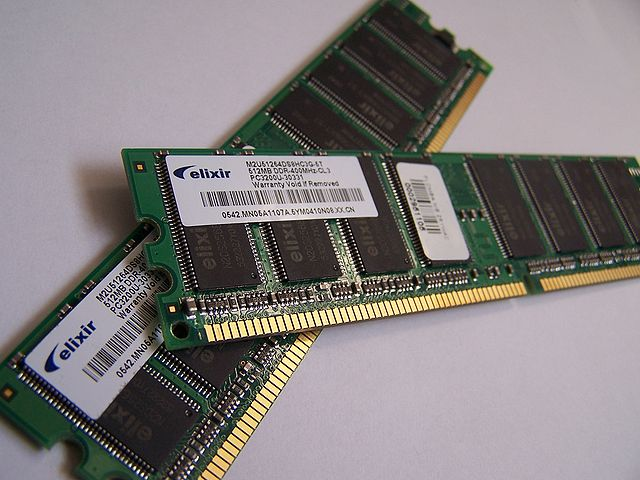
\includegraphics[height=11em]{figs/RAM.jpg}
\caption{Example processor and memory hardware.}
\label{fig.cpuram}
\end{center}
\end{figure}

Users generally see and interact with touchscreens, keyboards, and monitors, but it's the processors and memory that perform the actual computation.
Nowadays it's fairly standard, even for a smartphone, to have at least eight processors and four gigabytes (four billion cells) of memory.


\section{What is programming?}

\index{program}

A {\bf program} is a sequence of instructions that specifies how to perform a computation on computer hardware.
The computation might be something mathematical, like solving a system of equations or finding the roots of a polynomial.
It could also be a symbolic computation, like searching and replacing text in a document or (strangely enough) compiling a program.

The details look different in different languages, but a few basic instructions appear in just about every language:

\begin{description}
\item[input:] Get data from the keyboard, a file, a sensor, or some other device.
\item[output:] Display data on the screen, or send data to a file or other device.
\item[math:] Perform basic mathematical operations like addition and division.
\item[decisions:] Check for certain conditions and execute the appropriate code.
\item[repetition:] Perform some action repeatedly, usually with some variation.
\end{description}

\index{programming}

Believe it or not, that's pretty much all there is to it.
Every program you've ever used, no matter how complicated, is made up of small instructions that look much like these.
So you can think of {\bf programming} as the process of breaking down a large, complex task into smaller and smaller subtasks.
The process continues until the subtasks are simple enough to be performed with the electronic circuits provided by the hardware.


\section{The hello world program}
\label{hello}

Traditionally, the first program you write when learning a new programming language is called the hello world program.
All it does is output the words ``Hello, World!''\ to the screen.
In Java, it looks like this:

% NOTE(ABD): I changed a lot of ``print'' to ``display'', partly to be
% more precise, but also to reduce the number of times ``print'' appears,
% which is a lot!

\index{Hello.java}

% height = 130 + 15 * num_lines
\begin{trinket}[235]{Hello.java}
public class Hello {

    public static void main(String[] args) {
        // generate some simple output
        System.out.println("Hello, World!");
    }
}
\end{trinket}

When this program runs it displays:

\begin{stdout}
Hello, World!
\end{stdout}

Notice that the output does not include the quotation marks.

%\index{public}
%\index{static}
%The word \java{public} means the code can be accessed from other source files.
%The word \java{static} means that memory is allocated for the program in advance.

%Unfortunately, this simple example uses language features (like \java{public} and \java{static}) that are hard to explain.
%In fact, we won't be able to explain all of them for several more chapters.
%But we can start with the structure.

\index{statement}
\index{print statement}

Java programs are made up of {\em class} and {\em method} definitions, and methods are made up of {\em statements}.
A {\bf statement} is a line of code that performs a basic action.
In the hello world program, this line is a {\bf print statement} that displays a message on the screen:

\begin{code}
System.out.println("Hello, World!");
\end{code}

\index{println}
\index{semicolon}
\index{; semicolon}

\java{System.out.println} displays results on the screen; the name \java{println} stands for ``print line''.
Confusingly, {\em print} can mean both ``display on the screen'' and ``send to the printer''.
In this book, we'll try to say ``display'' when we mean output to the screen.
Like most statements, the print statement ends with a semicolon (\java{;}).

\index{case-sensitive}

Java is ``case-sensitive'', which means that uppercase and lowercase are not the same.
In this example, \java{System} has to begin with an uppercase letter; \java{system} and \java{SYSTEM} won't work.

\index{method}

A {\bf method} is a named sequence of statements.
This program defines one method named \java{main}:

\begin{code}
public static void main(String[] args)
\end{code}

\index{main}

The name and format of \java{main} is special: when the program runs, it starts at the first statement in \java{main} and ends when it finishes the last statement.
Later, we will see programs that define more than one method.

\index{class}

A {\bf class} is a collection of methods.
This program defines a class named \java{Hello}.
You can give a class any name you like, but it is conventional to start with a capital letter.
The name of the class has to match the name of the file it is in, so this class has to be in a file named {\tt Hello.java}.

\index{\{\} curly braces}
\index{brackets!curly}

Java uses curly braces (\{ and \}) to group things together.
In {\tt Hello.java}, the outermost braces contain the class definition, and the inner braces contain the method definition.

\index{comment!end-of-line}
\index{statement!comment}

The line that begins with two slashes (\java{//}) is a {\bf comment}, which is a bit of English text that explains the code.
When Java sees \java{//}, it ignores everything from there until the end of the line.
Comments have no effect on the execution of the program, but they make it easier for other programmers (and your future self) to understand what you meant to do.


\section{Compiling Java programs}

\index{high-level language}
\index{language!high-level}

The programming language you will learn in this book is Java, which is a {\bf high-level language}.
Other high-level languages you may have heard of include Python, C and C++, PHP, Ruby, and JavaScript.

\index{low-level language}
\index{language!low-level}

Before they can run, programs in high-level languages have to be translated into a {\bf low-level language}, also called ``machine language''.
This translation takes some time, which is a small disadvantage of high-level languages.
But high-level languages have two major advantages:

\begin{itemize}

\item It is {\em much} easier to program in a high-level language.
Programs take less time to write, they are shorter and easier to read, and they are more likely to be correct.

\index{portable}

\item High-level languages are {\bf portable}, meaning they can run on different kinds of computers with few or no modifications.
Low-level programs can only run on one kind of computer, and have to be rewritten to run on another.

\end{itemize}

\index{interpret}

Two kinds of programs translate high-level languages into low-level languages: interpreters and compilers.
An {\bf interpreter} reads a high-level program and executes it, meaning that it does what the program says.
It processes the program a little at a time, alternately reading lines and performing computations.
Figure~\ref{fig.interpreter} shows the structure of an interpreter.

\begin{figure}[!ht]
\begin{center}
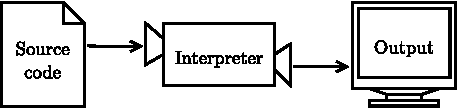
\includegraphics{figs/interpreter.pdf}
\caption{How interpreted languages are executed.}
\label{fig.interpreter}
\end{center}
\end{figure}

\index{compile}
\index{source code}
\index{object code}
\index{executable}

In contrast, a {\bf compiler} reads the entire program and translates it completely before the program starts running.
In this context, the high-level program is called the {\bf source code}, and the translated program is called the {\bf object code} or the {\bf executable}.
Once a program is compiled, you can execute it repeatedly without further translation.
As a result, compiled programs often run faster than interpreted programs.

\index{byte code}

Java is {\em both} compiled and interpreted.
Instead of translating programs directly into machine language, the Java compiler generates {\bf byte code}.
Similar to object code, byte code is easy and fast to interpret.
But it is also portable, so it is possible to compile a Java program on one machine, transfer the byte code to another machine, and run the byte code on the other machine.
This ability is an advantage of Java over some other high-level languages.

\index{javac}
\index{virtual machine}
\index{JVM}

Figure~\ref{fig.compiler} shows the steps of the development process.
The Java compiler is a program named {\tt javac}.
It translates {\tt .java} files into {\tt .class} files that store the resulting byte code.
The Java interpreter is a program named {\tt java}, which is short for ``Java Virtual Machine'' (JVM).

\begin{figure}[!ht]
\begin{center}
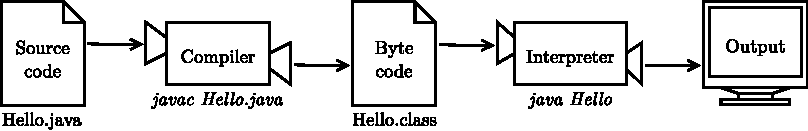
\includegraphics{figs/compiler.pdf}
\caption{The process of compiling and running a Java program.}
\label{fig.compiler}
\end{center}
\end{figure}

The programmer writes source code in the file {\tt Hello.java} and uses {\tt javac} to compile it.
If there are no errors, the compiler saves the byte code in the file {\tt Hello.class}.
To run the program, the programmer uses {\tt java} to interpret the byte code.
The result of the program is then displayed on the screen.

Although it might seem complicated, these steps are automated for you in most program development environments.
Usually you only have to press a button or type a single command to compile and run your program.
On the other hand, it is important to know what steps are happening in the background, so if something goes wrong you can figure out what it is.


\section{Displaying two messages}

You can put as many statements as you like in the \java{main} method.
For example, to display more than one line of output:

\begin{trinket}[250]{Hello2.java}
public class Hello2 {

    public static void main(String[] args) {
        // generate some simple output
        System.out.println("Hello, World!");  // first line
        System.out.println("How are you?");   // another line
    }
}
\end{trinket}

As this example shows, you can put comments at the end of a line as well as on lines all by themselves.

\index{quote mark}
\index{string}
\index{type!String}
\index{char}

Phrases that appear in quotation marks are called {\bf strings}, because they contain a sequence of characters strung together in memory.
Characters can be letters, numbers, punctuation marks, symbols, spaces, tabs, etc.

\index{newline}
\index{print}
\index{statement!print}

\java{System.out.println} appends a special character, called a {\bf newline}, that moves to the beginning of the next line.
If you don't want a newline at the end, you can use \java{print} instead of \java{println}:

\index{Goodbye.java}

\begin{trinket}[235]{Goodbye.java}
public class Goodbye {

    public static void main(String[] args) {
        System.out.print("Goodbye, ");
        System.out.println("cruel world");
    }
}
\end{trinket}

\label{goodbye}

In this example, the first statement does not add a newline, so the output appears on a single line as {\tt Goodbye, cruel world}.
Notice that there is a space at the end of the first string, which appears in the output just before the word cruel.


\section{Formatting source code}
\label{formatting}

In Java source code, some spaces are required.
For example, you need at least one space between words, so this program is not legal:

\begin{code}
publicclassGoodbye{

    publicstaticvoidmain(String[] args) {
        System.out.print("Goodbye, ");
        System.out.println("cruel world");
    }
}
\end{code}

But most other spaces are optional.
For example, this program {\em is} legal:

\begin{trinket}[220]{Goodbye.java}
public class Goodbye {
public static void main(String[] args) {
System.out.print("Goodbye, ");
System.out.println("cruel world");
}
}
\end{trinket}

The newlines are optional, too.
So we could just write:

\begin{trinket}[175]{Goodbye.java}
public class Goodbye { public static void main(String[] args)
{ System.out.print("Goodbye, "); System.out.println
("cruel world");}}
\end{trinket}

It still works, but the program is getting harder and harder to read.
Newlines and spaces are important for organizing your program visually, making it easier to understand the program and find errors when they occur.

Many editors will automatically format source code with consistent indenting and line breaks.
For example, in DrJava (see Appendix~\ref{drjava}) you can indent your code by selecting all text ({\sf Ctrl+A}) and pressing the {\sf Tab} key.


%\section{Style guidelines}

%\index{whitespace}
%
%As we saw in Section~\ref{formatting}, the compiler generally ignores spaces, tabs, and newlines.
%These characters, which are called {\bf whitespace}, affect the format of the code, but they don't affect its behavior.

%You have a lot of freedom in how you arrange your code.
%However, with that freedom comes responsibility, both to yourself (when you look at the code in the future) and others who will be reading, understanding, and debugging it.

\index{Google style}
\index{style guide}

Organizations that do a lot of software development usually have strict guidelines on how to format source code.
For example, Google publishes its Java coding standards for use in open-source projects: \url{https://google.github.io/styleguide/javaguide.html}.
%It is easier to understand a large codebase when all the source code is formatted consistently.
%Plus following style guidelines helps you to avoid common programming mistakes that are difficult to debug.

You probably won't understand these guidelines now, because they refer to language features we haven't yet seen.
But you might want to refer back to them periodically as you read this book.

%In the meantime, there are software tools that help programmers find and correct style issues.
%One of the most popular is Checkstyle, which enforces most of Google's guidelines.
%Instructions for downloading and running Checkstyle are in Appendix~\ref{checkstyle}.


\section{Escape sequences}

It's possible to display multiple lines of output with only one line of code.
You just have to tell Java where to put the line breaks.

\begin{trinket}[220]{Hello3.java}
public class Hello3 {

    public static void main(String[] args) {
        System.out.print("Hello!\nHow are you doing?\n");
    }
}
\end{trinket}

The output is two lines, each ending with a newline character:

\begin{stdout}
Hello!
How are you doing?
\end{stdout}

\index{escape sequence}

Each \verb"\n" is an {\bf escape sequence}, or two characters of source code that represent a single character.
(The backslash allows you to ``escape'' the string to write special characters.)
Notice there is no space between \verb"\n" and \verb"How".
If you add a space there, there will be a space at the beginning of the second line.

\begin{table}[!ht]
\begin{center}
\begin{tabular}{|c|c|}
\hline
\verb"\n" & newline \\
\hline
\verb"\t" & tab \\
\hline
\verb'\"' & double quote \\
\hline
\verb"\\" & backslash \\
\hline
\end{tabular}
\caption{Common escape sequences}
\label{tab:escape}
\end{center}
\end{table}

Java has a total of eight escape sequences, and the four most commonly used ones are listed in Table~\ref{tab:escape}.
For example, to write quotation marks inside of strings, you need to escape them with a backslash.

\begin{code}
System.out.println("She said \"Hello!\" to me.");
\end{code}

The result is:

\begin{stdout}
She said "Hello!" to me.
\end{stdout}


\section{What is computer science?}

This book intentionally omits some details about the Java language (such as the other escape sequences), because our main goal is learning how to think like a computer scientist.
Being able to understand computation is much more valuable than just learning how to write code.

If you're interested in learning more about Java itself, Oracle maintains an official set of tutorials on their website: \url{https://docs.oracle.com/javase/tutorial/}.
The ``Language Basics'' tutorial (found under ``Learning the Java Language'') is a good place to start.

One of the most interesting aspects of writing programs is deciding how to solve a particular problem, especially when there are multiple solutions.
For example, there are numerous ways to sort a list of numbers, and each way has its advantages.
%\href{https://www.toptal.com/developers/sorting-algorithms/}{\tt Sorting-algorithms.com} provides animations and descriptions for eight of the most common ways.
In order to determine which way is best for a given situation, we need techniques for describing and analyzing solutions formally.

\index{algorithm}
\index{computer science}

An {\bf algorithm} is a sequence of steps that specifies how to solve a problem.
Some algorithms are faster than others, and some use less space in computer memory.
{\bf Computer science} is the science of algorithms, including their discovery and analysis.
As you learn to develop algorithms for problems you haven't solved before, you will learn to think like a computer scientist.
%It's much more fun to discover new algorithms than to write the code for solutions that other people came up with!

\index{bug}
\index{debugging}

Designing algorithms and writing code is difficult and error-prone.
For historical reasons, programming errors are called {\bf bugs}, and the process of tracking them down and correcting them is called {\bf debugging}.
As you learn to debug your programs, you will develop new problem-solving skills.
You will need to think creatively when unexpected errors happen.

Although it can be frustrating, debugging is an intellectually rich, challenging, and interesting part of computer science.
In some ways, debugging is like detective work.
You are confronted with clues, and you have to infer the processes and events that led to the results you see.
Thinking about how to correct programs and improve their performance sometimes even leads to the discovery of new algorithms.


\section{Debugging programs}
\label{sec:examples}

It is a good idea to read this book in front of a computer so you can try out the examples as you go.
You can run many of the examples directly in DrJava's Interactions Pane (see Appendix~\ref{interactions}).
But if you put the code in a source file, it will be easier to try out variations.

\index{error!message}

Whenever you are experimenting with a new feature, you should also try to make mistakes.
For example, in the hello world program, what happens if you leave out one of the quotation marks?
What if you leave out both?
What if you spell \java{println} wrong?
These kinds of experiments help you remember what you read.
They also help with debugging, because you learn what the error messages mean.
It is better to make mistakes now and on purpose than later on and accidentally.

\index{experimental debugging}
\index{debugging!experimental}

%\index{Holmes, Sherlock}
%\index{Doyle, Arthur Conan}

Debugging is like an experimental science: once you have an idea about what is going wrong, you modify your program and try again.
If your hypothesis was correct, then you can predict the result of the modification, and you take a step closer to a working program.
If your hypothesis was wrong, you have to come up with a new one.
%As Sherlock Holmes pointed out, ``When you have eliminated the impossible, whatever remains, however improbable, must be the truth.''
%(A.~Conan Doyle, {\em The Sign of Four}.)

Programming and debugging should go hand in hand.
Don't just write a bunch of code and then perform trial and error debugging until it all works.
Instead, start with a program that does {\em something} and make small modifications, debugging them as you go, until the program does what you want.
That way you will always have a working program, and it will be easier to isolate errors.

\index{Linux}
\index{Torvalds, Linus}
\index{Greenfield, Larry}

A great example of this principle is the Linux operating system, which contains millions of lines of code.
It started out as a simple program Linus Torvalds used to explore the Intel 80386 chip.
According to Larry Greenfield in {\it The Linux Users' Guide}, ``One of Linus's earlier projects was a program that would switch between printing AAAA and BBBB.
This later evolved to Linux.''

%Later chapters will make more suggestions about debugging and other programming practices.

Finally, programming sometimes brings out strong emotions.
If you are struggling with a difficult bug, you might feel angry, despondent, or embarrassed.
Remember that you are not alone, and virtually every programmer has had similar experiences.
Don't hesitate to reach out to a friend and ask questions!


\section{Vocabulary}

Throughout the book, we try to define each term the first time we use it.
At the end of each chapter, we include the new terms and their definitions in order of appearance.
If you spend some time learning this vocabulary, you will have an easier time reading the following chapters.

\begin{description}

\term{problem solving}
The process of formulating a problem, finding a solution, and expressing the solution.

\term{hardware}
The electronic and mechanical components of a computer, such as CPUs, RAM, and hard disks.

\term{processor}
A computer chip that performs simple instructions like basic arithmetic and logic.

\term{memory}
Circuits that store data as long as the computer is turn on.
Not to be confused with permanent storage devices like hard disks and flash.

\term{program}
A sequence of instructions that specifies how to perform tasks on a computer.
Also known as software.

\term{programming}
The application of problem solving to creating executable computer programs.

\term{statement}
Part of a program that specifies one step of an algorithm.

\term{print statement}
A statement that causes output to be displayed on the screen.

\term{method}
A named sequence of statements.

\term{class}
For now, a collection of related methods.
(We will see later that there is a lot more to it.)

\term{comment}
A part of a program that contains information about the program but has no effect when the program runs.

\term{high-level language}
A programming language that is designed to be easy for humans to read and write.

\term{low-level language}
A programming language that is designed to be easy for a computer to run.
Also called ``machine language'' or ``assembly language''.

\term{portable}
The ability of a program to run on more than one kind of computer.

\term{interpret}
To run a program in a high-level language by translating it one line at a time and immediately executing the corresponding instructions.

\term{compile}
To translate a program in a high-level language into a low-level language, all at once, in preparation for later execution.

\term{source code}
A program in a high-level language, before being compiled.

\term{object code}
The output of the compiler, after translating the program.

\term{executable}
Another name for object code that is ready to run on specific hardware.

\term{byte code}
A special kind of object code used for Java programs.
Byte code is similar to a low-level language, but it is portable like a high-level language.

\term{string}
A sequence of characters; the primary data type for text.

\term{newline}
A special character signifying the end of a line of text.
Also known as line ending, end of line (EOL), or line break.

%\term{whitespace}
%Newlines, tab characters, and other spaces in a source program.
%Whitespace characters are used to separate words, but other than that, they don't affect the behavior of the program.

\term{escape sequence}
A sequence of code that represents a special character when used inside a string.

\term{algorithm}
A procedure or formula for solving a problem, with or without a computer.

\term{computer science}
The scientific and practical approach to computation and its applications.

\term{bug}
An error in a program.

\term{debugging}
The process of finding and removing errors.

\end{description}


\section{Exercises}

At the end of each chapter, we include exercises you can do with the things you've learned.
We encourage you to at least attempt every problem.
You can't learn to program only by reading about it; you have to practice.

Before you can compile and run Java programs, you might have to download and install a few tools.
There are many good options, but we recommend DrJava, which is an ``integrated development environment'' (IDE) well suited for beginners.
Instructions for getting started are in Appendix~\ref{tools}.

The code for this chapter is in the {\tt ch01} directory of {\tt ThinkJavaCode2}.
See page~\pageref{code} for instructions on how to download the repository.
Before you start the exercises, we recommend that you compile and run the examples.


\begin{exercise}  %%V6 Ex1.1

Computer scientists have the annoying habit of using common English words to mean something other than their common English meaning.
For example, in English, statements and comments are the same thing, but in programs they are different.

\begin{enumerate}
\item In computer jargon, what's the difference between a statement and a comment?
\item What does it mean to say that a program is portable?
\item In common English, what does the word compile mean?
\item What is an executable? Why is that word used as a noun?
\end{enumerate}

The glossary at the end of each chapter is intended to highlight words and phrases that have special meanings in computer science.
When you see familiar words, don't assume that you know what they mean!

\end{exercise}


\begin{exercise}  %%V6 Ex1.2

Before you do anything else, find out how to compile and run a Java program.
Some environments provide sample programs similar to the example in Section~\ref{hello}.

\begin{enumerate}
\item Type in the hello world program, then compile and run it.

\item Add a print statement that displays a second message after the ``Hello, World!''.
Say something witty like, ``How are you?''
Compile and run the program again.

\item Add a comment to the program (anywhere), recompile, and run it again.
The new comment should not affect the result.
\end{enumerate}

This exercise may seem trivial, but it is the starting place for many of the programs we will work with.
To debug with confidence, you will need to have confidence in your programming environment.

In some environments, it is easy to lose track of which program is executing.
You might find yourself trying to debug one program while you are accidentally running another.
Adding (and changing) print statements is a simple way to be sure that the program you are looking at is the program you are running.

\end{exercise}


\begin{exercise}  %%V6 Ex1.3

It is a good idea to commit as many errors as you can think of, so that you see what error messages the compiler produces.
Sometimes the compiler tells you exactly what is wrong, and all you have to do is fix it.
But sometimes the error messages are misleading.
Over time you will develop a sense for when you can trust the compiler and when you have to figure things out yourself.

Starting with the hello world program, try out each of the following errors.
After you make each change, compile the program, read the error message (if there is one), and then fix the error.

\begin{enumerate}
\item Remove one of the open curly braces.
\item Remove one of the close curly braces.
\item Instead of \java{main}, write \java{mian}.
\item Remove the word \java{static}.
\item Remove the word \java{public}.
\item Remove the word \java{System}.
\item Replace \java{println} with \java{Println}.
\item Replace \java{println} with \java{print}.
\item Delete one of the parentheses.
\item Add an extra parenthesis.
\end{enumerate}

\end{exercise}


\chapter{Variables and operators}

This chapter describes how to write statements using {\em variables}, which store values like numbers and words, and {\em operators}, which are symbols that perform a computation.
We also explain three kinds of programming errors and offer additional debugging advice.
%Understanding what can go wrong will help you get it right.
%Finally we discuss the rules of code style, which helps make programs easier to read and debug.

To run the examples in this chapter, you will need to create a new Java class with a \java{main} method (see Section~\ref{hello}).
We often omit the class and method definitions to keep the examples concise.


\section{Declaring variables}

%NOTE: in response to review comments, I am cleaning up the use of
% ``memory''.  I would like to avoid talking about hardware, or being
% specific about where values are stored.  The addresses that appear
% as object IDs are actually virtual addresses; the values themselves
% might be in RAM or on HDD.  But we really don't want to get into
% that.  I'd rather offer the abstract model that a variable indicates
% a location that contains a value.

\index{variable}
\index{value}

One of the most powerful features of a programming language is the ability to define and manipulate {\bf variables}.
A variable is a named location in memory that stores a {\bf value}.
Values may be numbers, text, images, sounds, and other types of data.
%They can be printed, and as we'll see later, operated on.
To store a value, you first have to declare a variable.
%Since the values we want to store are text, we declare that the new variable is a string:

\begin{code}
String message;
\end{code}

\index{declaration}
\index{statement!declaration}
\index{type!int}
\index{type!char}
\index{type!String}

This statement is called a {\bf declaration}, because it declares that the variable named \java{message} has the type \java{String}.
Each variable has a {\bf type} that determines what kind of values it can store.
For example, the \java{int} type can store integers, and the \java{char} type can store characters.

Some types begin with a capital letter and some with lowercase.
We will learn the significance of this distinction later, but for now you should take care to get it right.
There is no such type as \java{Int} or \java{string}.
%, and the compiler will complain if you make one up.

To declare an integer variable named \java{x}, you simply type:

\begin{code}
int x;
\end{code}

Note that \java{x} is an arbitrary name for the variable.
In general, you should use names that indicate what the variables mean.
%For example, if you saw these declarations, you could probably guess what values would be stored:

\begin{code}
String firstName;
String lastName;
int hour, minute;
\end{code}

This example declares two variables with type \java{String} and two with type \java{int}.
The last line shows how to declare multiple variables with the same type: \java{hour} and \java{minute} are both integers.
Note that each declaration statement ends with a semicolon (\java{;}).

\index{case-sensitive}

Variable names usually begin with a lowercase letter, in contrast to class names (like \java{Hello}) that start with a capital letter.
When a variable name contains more than one word (like \java{firstName}), it is conventional to capitalize the first letter of each subsequent word.
Variable names are case-sensitive, so \java{firstName} is not the same as \java{firstname} or \java{FirstName}.

\index{keyword}

You can use any name you want for a variable.
But there are about 50 reserved words, called {\bf keywords}, that you are not allowed to use as variable names.
These words include \java{public}, \java{class}, \java{static}, \java{void}, and \java{int}, which are used by the compiler to analyze the structure of the program.

You can find the complete list of keywords at \url{http://docs.oracle.com/javase/tutorial/java/nutsandbolts/_keywords.html}, but you don't have to memorize them.
Most programming editors provide ``syntax highlighting'', which makes different parts of the program appear in different colors.
%For example, keywords are often blue, strings red, comments green, and other code black.
%If you type a variable name and it turns blue, watch out!


\section{Assigning variables}

\index{assignment}
\index{= assignment operator}
\index{statement!assignment}

Now that we have declared some variables, we can use them to store values.
We do that with an {\bf assignment} statement.

\begin{code}
message = "Hello!";  // give message the value "Hello!"
hour = 11;           // assign the value 11 to hour
minute = 59;         // set minute to 59
\end{code}

This example shows three assignments, and the comments illustrate different ways people sometimes talk about assignment statements.
The vocabulary can be confusing here, but the idea is straightforward:

\begin{itemize}
\item When you declare a variable, you create a named storage location.
\item When you make an assignment to a variable, you update its value.
\end{itemize}

As a general rule, a variable has to have the same type as the value you assign to it.
For example, you cannot store a string in \java{minute} or an integer in \java{message}.
We will see some examples that seem to break this rule, but we'll get to that later.

%On the other hand, that rule can be confusing.
%There are many ways that you can convert values from one type to another, and Java sometimes converts things automatically.
%For now you should remember the general rule, and we'll talk about exceptions later.

A common source of confusion is that some strings {\em look} like integers, but they are not.
For example, \java{message} can contain the string \java{"123"}, which is made up of the characters \java{'1'}, \java{'2'}, and \java{'3'}.
But that is not the same thing as the integer \java{123}.

\begin{code}
message = "123";     // legal
message = 123;       // not legal
\end{code}

\index{initialize}

Variables must be {\bf initialized} (assigned for the first time) before they can be used.
You can declare a variable and then assign a value later, as in the previous example.
You can also declare and initialize on the same line:

\begin{code}
String message = "Hello!";
int hour = 11;
int minute = 59;
\end{code}

%You can make more than one assignment to the same variable.
%For example:
%
%\begin{code}
%int i = 1;
%i = 2;
%\end{code}
%
%\index{update}
%
%The first line initializes \java{i} to 1.
%The second line changes its value to \java{2}.
%In this example, there is no reason to make two assignments, but in many programs it is useful to reassign, or {\bf update}, variables.


\section{Memory diagrams}
\label{state}

Because Java uses the \java{=} symbol for assignment, it is tempting to interpret the statement \java{a = b} as a statement of equality.
It is not!

Equality is commutative, and assignment is not.
For example, in mathematics if $a = 7$ then $7 = a$.
In Java \java{a = 7;} is a legal assignment statement, but \java{7 = a;} is not.
The left side of an assignment statement has to be a variable name (storage location).

Also, in mathematics, a statement of equality is true for all time.
If $a = b$ now, $a$ is always equal to $b$.
In Java, an assignment statement can make two variables equal, but they don't have to stay that way.

\begin{code}
int a = 5;
int b = a;     // a and b are now equal
a = 3;         // a and b are no longer equal
\end{code}

The third line changes the value of \java{a}, but it does not change the value of \java{b}, so they are no longer equal.

\index{state}

Taken together, the variables in a program and their current values make up the program's {\bf state}.
Figure~\ref{fig.state} shows the state of the program after these assignment statements run.

\begin{figure}[!ht]
\begin{center}
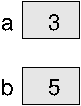
\includegraphics{figs/state.pdf}
\caption{Memory diagram of the variables \java{a} and \java{b}.}
\label{fig.state}
\end{center}
\end{figure}

\index{memory diagram}
\index{diagram!memory}

Diagrams like this one that show the state of the program are called {\bf memory diagrams}.
Each variable is represented with a box showing the name of the variable on the outside and the value inside.
As the program runs, the state of memory changes, so memory diagrams only show a particular point in time.


\section{Printing variables}
\label{sec:printvar}

You can display the current value of a variable using \java{print} or \java{println}.
The following statements declare a variable named \java{firstLine}, assign it the value \java{"Hello, again!"}, and display that value.

\begin{code}
String firstLine = "Hello, again!";
System.out.println(firstLine);
\end{code}

%Assuming this code fragment is inside a method that is inside a class, the output is:
%
%\begin{stdout}
%Hello, again!
%\end{stdout}

When we talk about displaying a variable, we generally mean the {\em value} of the variable.
To display the {\em name} of a variable, you have to put it in quotes.
%For example: \java{System.out.println("firstLine");}

\begin{code}
System.out.print("The value of firstLine is ");
System.out.println(firstLine);
\end{code}

For this example, the output is:

\begin{stdout}
The value of firstLine is Hello, again!
\end{stdout}

Conveniently, the code for displaying a variable is the same regardless of its type.
For example:

\begin{code}
int hour = 11;
int minute = 59;
System.out.print("The current time is ");
System.out.print(hour);
System.out.print(":");
System.out.print(minute);
System.out.println(".");
\end{code}

The output of this program is:

\begin{stdout}
The current time is 11:59.
\end{stdout}

To output multiple values on the same line, it's common to use several \java{print} statements followed by \java{println} at the end.
But don't forget the \java{println}!
On many computers, the output from \java{print} is stored without being displayed until \java{println} is run; then the entire line is displayed at once.
If you omit the \java{println}, the program might display the stored output at unexpected times or even terminate without displaying anything.


\section{Arithmetic operators}

%Recall that Java programs are organized into {\em classes}, each of which has one or more {\em methods}, each of which has one or more {\em statements}.
%Most statements consist of one or more {\bf expressions}.

\index{operator}
\index{addition!integer}

{\bf Operators} are symbols that represent simple computations.
%Most operators in Java do what you expect them to do, since they are common mathematical symbols.
For example, the addition operator is \java{+}, subtraction is \java{-}, multiplication is \java{*}, and division is \java{/}.
%Variables are replaced with their values before the computation is performed.

The following program converts a time of day to minutes:

\begin{code}
int hour = 11;
int minute = 59;
System.out.print("Number of minutes since midnight: ");
System.out.println(hour * 60 + minute);
\end{code}

The output is:

\begin{stdout}
Number of minutes since midnight: 719
\end{stdout}

\index{expression}
\index{operand}

In this program, \java{hour * 60 + minute} is an {\bf expression}, which represents a single value to be computed (\java{719}).
When the program runs, each variable is replaced by its current value, and then the operators are applied.
The values that operators work with are called {\bf operands}.

Expressions are generally a combination of numbers, variables, and operators.
When compiled and executed, they become a single value.
For example, the expression \java{1 + 1} has the value \java{2}.
In the expression \java{hour - 1}, Java replaces the variable with its value, yielding \java{11 - 1}, which has the value \java{10}.

In the expression \java{hour * 60 + minute}, both variables get replaced, yielding \java{11 * 60 + 59}.
The multiplication happens first, yielding \java{660 + 59}.
Then the addition yields \java{719}.

Addition, subtraction, and multiplication all do what you expect, but you might be surprised by division.
For example, the following fragment tries to compute the fraction of an hour that has elapsed:%, but it has a logic error:

\begin{code}
System.out.print("Fraction of the hour that has passed: ");
System.out.println(minute / 60);
\end{code}

The output is:

\begin{stdout}
Fraction of the hour that has passed: 0
\end{stdout}

\index{division!integer}
\index{integer division}

This result often confuses people.
The value of \java{minute} is 59, and 59 divided by 60 should be 0.98333, not 0.
The problem is that Java performs ``integer division'' when the operands are integers.
By design, integer division always rounds toward zero, even in cases like this one where the next integer is close.

As an alternative, we can calculate a percentage rather than a fraction:

\begin{code}
System.out.print("Percent of the hour that has passed: ");
System.out.println(minute * 100 / 60);
\end{code}

The new output is:

\begin{stdout}
Percent of the hour that has passed: 98
\end{stdout}

Again the result is rounded down, but at least now it's approximately correct.
%To get a more precise answer, we can use a different type of variable that can store fractional values.


\section{Floating-point numbers}

\index{floating-point}
\index{double}
\index{type!double}

A more general solution is to use {\bf floating-point} numbers, which can represent fractions as well as integers.
%As the name implies, the decimal point floats around (i.e., you can have as many decimal places as you want).
In Java, the default floating-point type is called \java{double}, which is short for double-precision.
You can create \java{double} variables and assign values to them the same way we did for the other types:

\begin{code}
double pi;
pi = 3.14159;
\end{code}

Java performs ``floating-point division'' when one or more operands are \java{double} values.
So we can solve the problem we saw in the previous section:

\begin{code}
double minute = 59.0;
System.out.print("Fraction of the hour that has passed: ");
System.out.println(minute / 60.0);
\end{code}

The output is:

\begin{stdout}
Fraction of the hour that has passed: 0.9833333333333333
\end{stdout}

Although floating-point numbers are useful, they can be a source of confusion.
For example, Java distinguishes the integer value \java{1} from the floating-point value \java{1.0}, even though they seem to be the same number.
They belong to different data types, and strictly speaking, you are not allowed to make assignments between types.

The following is illegal because the variable on the left is an \java{int} and the value on the right is a \java{double}:

\begin{code}
int x = 1.1;  // compiler error
\end{code}

It is easy to forget this rule, because in many cases Java {\em automatically} converts from one type to another:

\begin{code}
double y = 1;  // legal, but bad style
\end{code}

The preceding example should be illegal, but Java allows it by converting the \java{int} value \java{1} to the \java{double} value \java{1.0} automatically.
This leniency is convenient, but it often causes problems for beginners.
For example:

\begin{code}
double y = 1 / 3;  // common mistake
\end{code}

\index{division!integer}
\index{integer division}

You might expect the variable \java{y} to get the value \java{0.333333}, which is a legal floating-point value.
But instead it gets the value \java{0.0}.
The expression on the right divides two integers, so Java does integer division, which yields the \java{int} value \java{0}.
Converted to \java{double}, the value assigned to \java{y} is \java{0.0}.

One way to solve this problem (once you figure out the bug) is to make the right-hand side a floating-point expression.
The following sets \java{y} to \java{0.333333}, as expected:

\begin{code}
double y = 1.0 / 3.0;  // correct
\end{code}

As a matter of style, you should always assign floating-point values to floating-point variables.
The compiler won't make you do it, but you never know when a simple mistake will come back and haunt you.


\section{Rounding errors}

%The operations we have seen so far -- addition, subtraction, multiplication, and division -- also work on floating-point values, although you might be interested to know that the underlying mechanism is completely different.
%In fact, most processors have special circuitry just for performing floating-point operations.

Most floating-point numbers are only {\em approximately} correct.
Some numbers, like reasonably-sized integers, can be represented exactly.
But repeating fractions, like $1/3$, and irrational numbers, like $\pi$, cannot.
To represent these numbers, computers have to round off to the nearest floating-point number.

%Notwithstanding, there is a fundamental flaw with floating-point arithmetic.
%In mathematics, there is an infinite number of real numbers.
%But computer processors are finite; they cannot represent {\em every} possible floating-point number.
%Even with double-precision, you will frequently run into problems.

\index{rounding error}
\index{error!rounding}

The difference between the number we want and the floating-point number we get is called {\bf rounding error}.
For example, the following two statements should be equivalent:

\begin{code}
System.out.println(0.1 * 10);
System.out.println(0.1 + 0.1 + 0.1 + 0.1 + 0.1
                 + 0.1 + 0.1 + 0.1 + 0.1 + 0.1);
\end{code}

But on many machines, the output is:

\begin{stdout}
1.0
0.9999999999999999
\end{stdout}

The problem is that \java{0.1}, which is a terminating fraction in decimal, is a repeating fraction in binary.
So its floating-point representation is only approximate.
When we add up the approximations, the rounding errors accumulate.

For many applications, like computer graphics, encryption, statistical analysis, and multimedia rendering, floating-point arithmetic has benefits that outweigh the costs.
But if you need {\em absolute} precision, use integers instead.
For example, consider a bank account with a balance of \$123.45:

\begin{code}
double balance = 123.45;  // potential rounding error
\end{code}

In this example, balances will become inaccurate over time as the variable is used in arithmetic operations like deposits and withdrawals.
The result would be angry customers and potential lawsuits.
You can avoid the problem by representing the balance as an integer:

\begin{code}
int balance = 12345;      // total number of cents
\end{code}

\index{type!long}

This solution works as long as the number of cents doesn't exceed the largest integer, which is about 2 billion.
%If necessary you can use \java{long} instead, which has a max value of $2^{63}-1$ (about 92 quadrillion dollars).
%Hopefully nobody will ever need that much money!


\section{Operators for strings}

\index{string!operator}
\index{operator!string}

In general, you cannot perform mathematical operations on strings, even if the strings look like numbers.
The following expressions are illegal:

\begin{code}
"Hello" - 1     "World" / 123     "Hello" * "World"
\end{code}

\index{concatenate}
\index{addition!string}

The \java{+} operator works with strings, but it might not do what you expect.
For strings, the \java{+} operator performs {\bf concatenation}, which means joining end-to-end.
So \java{"Hello, " + "World!"} yields the string \java{"Hello, World!"}.

Likewise if you have a variable called \java{name} that has type \java{String}, the expression \java{"Hello, " + name} appends the value of \java{name} to the hello string, which creates a personalized greeting.

Since addition is defined for both numbers and strings, Java performs automatic conversions you may not expect:

\begin{code}
System.out.println(1 + 2 + "Hello");
// the output is 3Hello

System.out.println("Hello" + 1 + 2);
// the output is Hello12
\end{code}

Java executes these operations from left to right.
In the first line, \java{1 + 2} is \java{3}, and \java{3 + "Hello"} is \java{"3Hello"}.
But in the second line, \java{"Hello" + 1} is \java{"Hello1"}, and \java{"Hello1" + 2} is \java{"Hello12"}.


%\section{Order of operations}

\index{order of operations}
\index{precedence}

When more than one operator appears in an expression, they are evaluated according to the {\bf order of operations}.
Generally speaking, Java evaluates operators from left to right (as we saw in the previous section).
But for numeric operators, Java follows mathematical conventions:

\begin{itemize}

\item Multiplication and division take ``precedence'' over addition and subtraction, which means they happen first.
So \java{1 + 2 * 3} yields 7, not 9, and \java{2 + 4 / 2} yields 4, not 3.

\item If the operators have the same precedence, they are evaluated from left to right.
So in the expression \java{minute * 100 / 60}, the multiplication happens first; if the value of \java{minute} is 59, we get \java{5900 / 60}, which yields \java{98}.
If these same operations had gone from right to left, the result would have been \java{59 * 1}, which is incorrect.

\index{parentheses}
\index{( ) parentheses}

\item Any time you want to override the order of operations (or you are not sure what it is) you can use parentheses.
Expressions in parentheses are evaluated first, so \java{(1 + 2) * 3} is 9.
You can also use parentheses to make an expression easier to read, as in \java{(minute * 100) / 60}, even though it doesn't change the result.

\end{itemize}

See the Java tutorials for a complete table of operator precedence: \url{https://docs.oracle.com/javase/tutorial/java/nutsandbolts/operators.html}.
If the order of operations is not obvious when looking at an expression, you can always add parentheses to make it more clear.
But over time, you should internalize these kinds of details about the Java language.


\section{Compiler error messages}

\index{error!message}

Three kinds of errors can occur in a program: compile-time errors, run-time errors, and logic errors.
It is useful to distinguish among them in order to track them down more quickly.

\index{compile-time error}
\index{error!compile-time}

{\bf Compile-time} errors occur when you violate the rules of the Java language.
For example, parentheses and braces have to come in matching pairs.
So \java{(1 + 2)} is legal, but \java{8)} is not.
In the latter case, the program cannot be compiled, and the compiler displays an error.

\index{error!message}

Error messages from the compiler usually indicate where in the program the error occurred, and sometimes they can tell you exactly what the error is.
As an example, let's get back to the hello world program from Section~\ref{hello}.

\begin{trinket}[235]{Hello.java}
public class Hello {

    public static void main(String[] args) {
        // generate some simple output
        System.out.println("Hello, World!");
    }
}
\end{trinket}

\index{semicolon}
\index{; semicolon}

If you forget the semicolon at the end of the print statement, you might get an error message like this:

\begin{stdout}
File: Hello.java  [line: 5]
Error: ';' expected
\end{stdout}

That's pretty good: the location of the error is correct, and the error message tells you what's wrong.
But error messages are not always easy to understand.
Sometimes the compiler reports the place in the program where the error was {\em detected}, not where it actually occurred.
And sometimes the description of the problem is more confusing than helpful.

For example, if you forget the closing brace at the end of \java{main} (line 6), you might get a message like this:

\begin{stdout}
File: Hello.java  [line: 7]
Error: reached end of file while parsing
\end{stdout}

\index{parse}

There are two problems here.
First, the error message is written from the compiler's point of view, not yours.
{\bf Parsing} is the process of reading a program before translating; if the compiler gets to the end of the file while still parsing, that means something was omitted.
But the compiler doesn't know what.
It also doesn't know where.
The compiler discovers the error at the end of the program (line 7), but the missing brace should be on the previous line.

Error messages contain useful information, so you should make an effort to read and understand them.
But don't take them too literally.
During the first few weeks of your programming career, you will probably spend a lot of time tracking down compile-time errors.
As you gain experience, you will make fewer mistakes and find them more quickly.


\section{Other types of errors}
%\subsection{Run-time errors}

\index{run-time error}
\index{error!run-time}
\index{exception}

The second type of error is a {\bf run-time error}, so-called because it does not appear until after the program has started running.
In Java, these errors occur while the interpreter is executing byte code and something goes wrong.
These errors are also called ``exceptions'' because they usually indicate that something unexpected has happened.

Run-time errors are rare in the simple programs you will see in the first few chapters, so it might be a while before you encounter one.
When a run-time error occurs, the interpreter displays an error message that explains what happened and where.
For example, if you accidentally divide by zero you will get a message like:

\begin{small}
\begin{stdout}
Exception in thread "main" java.lang.ArithmeticException: / by zero
    at Hello.main(Hello.java:5)
\end{stdout}
\end{small}

\index{ArithmeticException}
\index{exception!Arithmetic}

Error messages are very useful for debugging.
The first line includes the name of the exception, \java{java.lang.ArithmeticException}, and a message that indicates more specifically what happened, \java{/ by zero}.
The next line shows the method where the error occurred; \java{Hello.main} indicates the method \java{main} in the class \java{Hello}.
It also reports the file where the method is defined, {\tt Hello.java}, and the line number where the error occurred, \java{5}.

Sometimes error messages contain additional information that doesn't make sense.
It can be a challenge to figure out where to find the useful parts without being overwhelmed by extraneous information.
Keep in mind that the line where the program crashed may not be the line that needs to be corrected.

%\subsection{Logic errors}

\index{logic error}
\index{error!logic}

The third type of error is a {\bf logic error}.
%{\bf Semantics} pertains to the meaning of a program; that is, what it does when it runs.
If your program has a logic error, it will compile and run without generating error messages, but it will not do the right thing.
Instead, it will do exactly what you told it to do.
For example, here is a version of the hello world program with a logic error:

\index{Hello.java}

\begin{trinket}[235]{Hello.java}
public class Hello {

    public static void main(String[] args) {
        System.out.println("Hello, ");
        System.out.println("World!");
    }
}
\end{trinket}

This program compiles and runs just fine, but the output is:

\begin{stdout}
Hello,
World!
\end{stdout}

Assuming that we wanted the output on one line, this is not correct.
The problem is that the first line uses \java{println}, when we probably meant to use \java{print} (see the ``goodbye world'' example of Section~\ref{goodbye}).

Identifying logic errors can be hard because you have to work backwards, looking at the output of the program, trying to figure out why it is doing the wrong thing, and how to make it do the right thing.
Usually the compiler and the interpreter can't help you, since they don't know what the right thing is.


\section{Vocabulary}

\begin{description}

\term{variable}
A named storage location for values.
All variables have a type, which is declared when the variable is created.

\term{value}
A number, string, or other data that can be stored in a variable.
Every value belongs to a type (for example, \java{int} or \java{String}).

\term{type}
Mathematically speaking, a set of values.
The type of a variable determines which values it can have.

\term{declaration}
A statement that creates a new variable and specifies its type.

\term{keyword}
A reserved word used by the compiler to analyze programs.
You cannot use keywords (like \java{public}, \java{class}, and \java{void}) as variable names.

\term{assignment}
A statement that gives a value to a variable.

\term{initialize}
To assign a variable for the first time.

%\term{update}
%An assignment that changes the value of a variable.

\term{state}
The variables in a program and their current values.

\term{memory diagram}
A graphical representation of the state of a program at a point in time.

\term{operator}
A symbol that represents a computation like addition, multiplication, or string concatenation.

\term{operand}
One of the values on which an operator operates.
Most operators in Java require two operands.

\term{expression}
A combination of variables, operators, and values that represents a single value.
Expressions also have types, as determined by their operators and operands.

\term{floating-point}
A data type that represents numbers with an integer part and a fractional part.
In Java, the default floating-point type is \java{double}.

\term{rounding error}
The difference between the number we want to represent and the nearest floating-point number.

\term{concatenate}
To join two values, often strings, end-to-end.

\term{order of operations}
The rules that determine in what order expressions are evaluated.
Also known as ``operator precedence''.

\term{compile-time error}
An error in the source code that makes it impossible to compile.
Also called a ``syntax error''.

\term{parse}
To analyze the structure of a program; what the compiler does first.

\term{run-time error}
An error in a program that makes it impossible to run to completion.
Also called an ``exception''.

\term{logic error}
An error in a program that makes it do something other than what the programmer intended.

\end{description}


\section{Exercises}

The code for this chapter is in the {\tt ch02} directory of {\tt ThinkJavaCode2}.
See page~\pageref{code} for instructions on how to download the repository.
Before you start the exercises, we recommend that you compile and run the examples.

If you have not already read Appendix~\ref{interactions}, now might be a good time.
It describes the DrJava Interactions Pane, which is a useful way to develop and test short fragments of code without writing a complete class definition.


\begin{exercise}  %%V6 Ex2.1

If you are using this book in a class, you might enjoy this exercise.
Find a partner and play ``Stump the Chump'':

Start with a program that compiles and runs correctly.
One player looks away while the other player adds an error to the program.
Then the first player tries to find and fix the error.
You get two points if you find the error without compiling the program, one point if you find it using the compiler, and your opponent gets a point if you don't find it.

\end{exercise}


\begin{exercise}  %%V6 Ex2.2
\label{ex:date}

The point of this exercise is (1) to use string concatenation to display values with different types (\java{int} and \java{String}), and (2) to practice developing programs gradually by adding a few statements at a time.

\begin{enumerate}

\item Create a new program named {\tt Date.java}.
Copy or type in something like the hello world program and make sure you can compile and run it.

\item Following the example in Section~\ref{sec:printvar}, write a program that creates variables named \java{day}, \java{date}, \java{month}, and \java{year}.
The variable \java{day} will contain the day of the week (like Friday), and \java{date} will contain the day of the month (like the 13th).
%What type is each variable?
Assign values to those variables that represent today's date.

\item Display the value of each variable on a line by itself.
This is an intermediate step that is useful for checking that everything is working so far.
Compile and run your program before moving on.

\item Modify the program so that it displays the date in standard American format, for example: {\tt Thursday, July 16, 2015}.

\item Modify the program so it also displays the date in European format.
The final output should be:

\begin{stdout}
American format:
Thursday, July 16, 2015
European format:
Thursday 16 July 2015
\end{stdout}

%{\it Hint:} You should be able to copy, paste, and modify the code from Step 4 when completing Step 5.
\end{enumerate}

\end{exercise}


\begin{exercise}  %%V6 Ex2.3

The point of this exercise is to (1) use some of the arithmetic operators, and (2) start thinking about compound entities (like time of day) that are represented with multiple values.

\begin{enumerate}

\item Create a new program called {\tt Time.java}.
From now on, we won't remind you to start with a small, working program, but you should.

\item Following the example program in Section~\ref{sec:printvar}, create variables named \java{hour}, \java{minute}, and \java{second}.
Assign values that are roughly the current time.
Use a 24-hour clock so that at 2pm the value of \java{hour} is 14.

\item Make the program calculate and display the number of seconds since midnight.

\item Calculate and display the number of seconds remaining in the day.

\item Calculate and display the percentage of the day that has passed.
You might run into problems when computing percentages with integers, so consider using floating-point.

\item Change the values of \java{hour}, \java{minute}, and \java{second} to reflect the current time.
Then write code to compute the elapsed time since you started working on this exercise.

\end{enumerate}

{\it Hint:} You might want to use additional variables to hold values during the computation.
Variables that are used in a computation but never displayed are sometimes called ``intermediate'' or ``temporary'' variables.

\end{exercise}


\chapter{Input and output}

The programs we've looked at so far simply display messages, which doesn't really involve that much computation.
This chapter will show you how to read input from the keyboard, use that input to calculate a result, and then format that result for output.
%We will also look at some technical details about how operating systems work.


\section{The System class}

\index{class!System}

We have been using \java{System.out.println} for a while, but you might not have thought about what it means.
\java{System} is a class that provides methods related to the ``system'' or environment where programs run.
It also provides \java{System.out}, which is a special value that has additional methods (like \java{println}) for displaying output.

\index{System.out}

In fact, we can use \java{System.out.println} to display the value of \java{System.out}:

\begin{code}
System.out.println(System.out);
\end{code}

The result is:

\begin{stdout}
java.io.PrintStream@685d72cd
\end{stdout}

\index{package}
\index{java.io}

This output indicates that \java{System.out} is a \java{PrintStream}, which is defined in a package called \java{java.io}.
A {\bf package} is a collection of related classes; \java{java.io} contains classes for ``I/O'' which stands for input and output.

\index{address}
\index{hexadecimal}

The numbers and letters after the {\tt @} sign are the {\bf address} of \java{System.out}, represented as a hexadecimal (base 16) number.
The address of a value is its location in the computer's memory, which might be different on different computers.
In this example the address is \java{685d72cd}, but if you run the same code you will likely get something else.
%You can think of the address as a unique identifier for the object.

\index{library}

As shown in Figure~\ref{fig.system}, \java{System} is defined in a file called {\tt System.java}, and \java{PrintStream} is defined in {\tt PrintStream.java}.
These files are part of the Java {\bf library}, which is an extensive collection of classes that you can use in your programs.
The source code for these classes is usually included with the compiler (see Section~\ref{src.zip}).

\begin{figure}[!ht]
\begin{center}
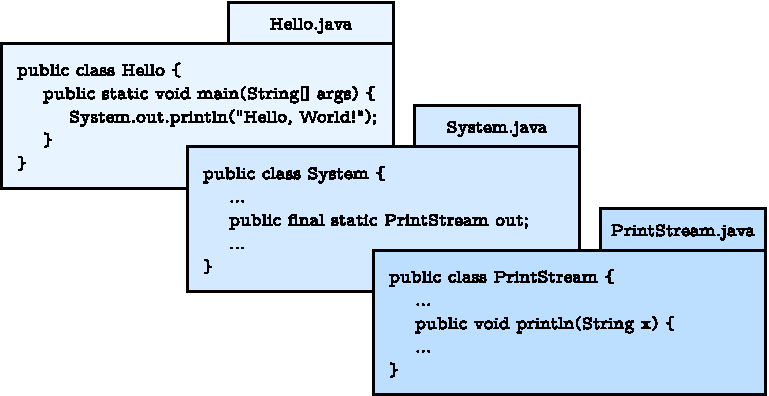
\includegraphics{figs/system.pdf}
\caption{\java{System.out.println} refers to the \java{out} variable of the \java{System} class, which is a \java{PrintStream} that provides a method called \java{println}.}
\label{fig.system}
\end{center}
\end{figure}


\section{The Scanner class}
\label{scanner}

\index{Scanner}
\index{class!Scanner}

%\index{byte}
%
%From the operating system's point of view, data from the keyboard arrives in a series of hardware control signals.
%The operating system translates these signals into a stream of {\bf bytes} (small integers), which in turn need to be translated into characters.
%\java{System.in} provides the means for reading one byte of input at a time, which is hardly useful for programs that would rather read in an entire word or line of input.

\index{System.in}

The \java{System} class also provides the special value \java{System.in}, which is an \java{InputStream} that has methods for reading input from the keyboard.
These methods are not convenient to use, but fortunately Java provides other classes that make it easy to handle common input tasks.

\index{class!utility}
\index{utility class}
\index{java.util}

For example, \java{Scanner} is a class that provides methods for inputting words, numbers, and other data.
\java{Scanner} is provided by \java{java.util}, which is a package that contains various ``utility classes''.
Before you can use \java{Scanner}, you have to import it like this:

\begin{code}
import java.util.Scanner;
\end{code}

\index{import statement}
\index{statement!import}

This {\bf import statement} tells the compiler that when you refer to \java{Scanner}, you mean the one defined in \java{java.util}.
Using an import statement is necessary because there might be another class named \java{Scanner} in another package.
%Using an import statement makes your code unambiguous.
Import statements can't be inside a class definition.
By convention, they are usually at the beginning of the file.

Next you have to initialize the \java{Scanner}.
This line declares a \java{Scanner} variable named \java{in} and creates a \java{Scanner} that reads input from \java{System.in}:
%We'll explain the \java{new} operator in more detail in Section~\ref{point}.

\begin{code}
Scanner in = new Scanner(System.in);
\end{code}

The \java{Scanner} class provides a method called \java{nextLine} that reads a line of input from the keyboard and returns a \java{String}.
The following example reads two lines and repeats them back to the user:

\index{Echo.java}

\begin{trinket}{Echo.java}
import java.util.Scanner;

public class Echo {

    public static void main(String[] args) {
        String line;
        Scanner in = new Scanner(System.in);

        System.out.print("Type something: ");
        line = in.nextLine();
        System.out.println("You said: " + line);

        System.out.print("Type something else: ");
        line = in.nextLine();
        System.out.println("You also said: " + line);
    }
}
\end{trinket}

If you omit the import statement at the top of the file, you will get a compiler error saying ``cannot find symbol''.
That means the compiler doesn't know where to find the definition for \java{Scanner}.

\index{java.lang}

You might wonder why we can use the \java{System} class without importing it.
\java{System} belongs to the \java{java.lang} package, which is imported automatically.
According to the documentation, \java{java.lang} ``provides classes that are fundamental to the design of the Java programming language.''
The \java{String} class is also part of the \java{java.lang} package.


\section{Language elements}

\index{language!elements}

At this point, we have seen nearly all of the organizational units that make up Java programs.
Figure~\ref{fig.package} shows how these ``language elements'' are related.

\begin{figure}[!ht]
\begin{center}
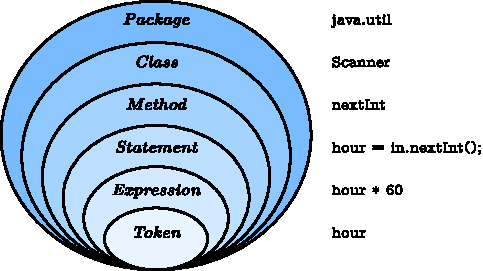
\includegraphics[width=4in]{figs/package.pdf}
\caption{Elements of the Java language, from largest to smallest.}
\label{fig.package}
\end{center}
\end{figure}

\index{token}

Java applications are typically organized into packages (like \java{java.io} and \java{java.util}) that include multiple classes (like \java{PrintStream} and \java{Scanner}).
Each class defines its own methods (like \java{println} and \java{nextLine}), and each method is a sequence of statements.

Each statement performs one or more computations, depending on how many expressions it has, and each expression represents a single value to compute.
For example, the assignment statement \java{hours = minutes / 60.0;} contains a single expression: \java{minutes / 60.0}.

{\bf Tokens} are the most basic elements of a program, including numbers, variable names, operators, keywords, parentheses, braces, and semicolons.
In the previous example, the tokens are \java{hours}, \java{=}, \java{minutes}, \java{/}, \java{60.0}, and \java{;} (spaces are ignored by the compiler).

%\index{syntax}
%\index{semantics}

Knowing this terminology is helpful, because error messages often say things like ``not a statement'' or ``illegal start of expression'' or ``unexpected token''.
Comparing Java to English, statements are complete sentences, expressions are phrases, and tokens are individual words and punctuation marks.

Note there is a big difference between the Java {\em language}, which defines the elements in Figure~\ref{fig.package}, and the Java {\em library}, which provides the built-in classes that you can import.
For example, the keywords \java{public} and \java{class} are part of the Java language, but the names \java{PrintStream} and \java{Scanner} are not.

The standard edition of Java comes with {\em several thousand} classes you can use, which can be both exciting and intimidating.
You can browse this library at \url{http://docs.oracle.com/javase/8/docs/api/}.
Interestingly, most of the Java library is written in Java.


%\section{Inches to centimeters}
\section{Literals and constants}

%Now let's work through an example that's a little more useful.
Although most of the world has adopted the metric system for weights and measures, some countries are stuck with Imperial units.
For example, when talking with friends in Europe about the weather, people in the United States might have to convert from Celsius to Fahrenheit and back.
%And when making an international purchase online, you may have to convert your nation's currency into another based on the exchange rate.
Or they might want to convert height in inches to centimeters.

%An everyday problem that computers are great at solving is converting numbers from one unit into another.
%For the rest of the chapter, we will look at how to write programs that solve these types of problems.
%Specifically, each program will 1) prompt the user for input, 2) read input from the keyboard, 3) calculate a result, and 4) format the result for output.
%The focus will not only be on Java syntax and language features, but also on the {\em process} of solving the problem, documenting the code, and testing the solution.

We can write a program to help.
We'll use a \java{Scanner} to input a measurement in inches, convert to centimeters, and then display the results.
The following lines declare the variables and create the \java{Scanner}:

\begin{code}
int inch;
double cm;
Scanner in = new Scanner(System.in);
\end{code}

\index{prompt}
\index{nextInt!Scanner}

The next step is to prompt the user for the input.
We'll use \java{print} instead of \java{println} so they can enter the input on the same line as the {\bf prompt}.
And we'll use the \java{Scanner} method \java{nextInt}, which reads input from the keyboard and converts it to an integer:

\begin{code}
System.out.print("How many inches? ");
inch = in.nextInt();
\end{code}

Next we multiply the number of inches by 2.54, since that's how many centimeters there are per inch, and display the results:

\begin{code}
cm = inch * 2.54;
System.out.print(inch + " in = ");
System.out.println(cm + " cm");
\end{code}

This code works correctly, but it has a minor problem.
If another programmer reads this code, they might wonder where 2.54 comes from.
For the benefit of others (and yourself in the future), it would be better to assign this value to a variable with a meaningful name.
%We'll demonstrate in the next section.


%\section{Literals and constants}

\index{literal}

A value that appears in a program, like the number 2.54, is called a {\bf literal}.
In general, there's nothing wrong with literals.
But when numbers like 2.54 appear in an expression with no explanation, they make the code hard to read.
And if the same value appears many times and could change in the future, it makes the code hard to maintain.

\index{magic number}

Values like 2.54 are sometimes called {\bf magic numbers} (with the implication that being ``magic'' is not a good thing).
A good practice is to assign magic numbers to variables with meaningful names, like this:

\begin{code}
double cmPerInch = 2.54;
cm = inch * cmPerInch;
\end{code}

This version is easier to read and less error-prone, but it still has a problem.
Variables can vary (hence the term), but the number of centimeters in an inch does not.
Once we assign a value to \java{cmPerInch}, it should never change.
Java provides the keyword \java{final}, a language feature that enforces this rule.

\begin{code}
final double CM_PER_INCH = 2.54;
\end{code}

\index{final}
\index{constant}

Declaring that a variable is \java{final} means that it cannot be reassigned once it has been initialized.
If you try, the compiler gives an error.
Variables declared as \java{final} are called {\bf constants}.
By convention, names for constants are all uppercase, with the underscore character (\java{_}) between words.


\section{Formatting output}
\label{printf}

When you output a \java{double} using \java{print} or \java{println}, it displays up to 16 decimal places:

\begin{code}
System.out.print(4.0 / 3.0);
\end{code}

The result is:

\begin{stdout}
1.3333333333333333
\end{stdout}

\index{printf}

That might be more than you want.
\java{System.out} provides another method, called \java{printf}, that gives you more control of the format.
The ``f'' in \java{printf} stands for ``formatted''.
Here's an example:

\begin{code}
System.out.printf("Four thirds = %.3f", 4.0 / 3.0);
\end{code}

\index{format string}
\index{format specifier}

The first value in the parentheses is a {\bf format string} that specifies how the output should be displayed.
This format string contains ordinary text followed by a {\bf format specifier}, which is a special sequence that starts with a percent sign.
The format specifier \java{\%.3f} indicates that the following value should be displayed as floating-point, rounded to three decimal places.
The result is:

\begin{stdout}
Four thirds = 1.333
\end{stdout}

The format string can contain any number of format specifiers; here's an example with two of them:

\begin{code}
int inch = 100;
double cm = inch * CM_PER_INCH;
System.out.printf("%d in = %f cm\n", inch, cm);
\end{code}

The result is:

\begin{stdout}
100 in = 254.000000 cm
\end{stdout}

Like \java{print}, \java{printf} does not append a newline.
So format strings often end with a newline character.

The format specifier \java{\%d} displays integer values (``d'' stands for ``decimal'', not double).
The values are matched up with the format specifiers in order, so \java{inch} is displayed using \java{\%d}, and \java{cm} is displayed using \java{\%f}.

Learning about format strings is like learning a sub-language within Java.
There are many options, and the details can be overwhelming.
Table~\ref{tab:format} lists a few common uses, to give you an idea of how things work.

\begin{table}[!ht]
\begin{center}
\begin{tabular}{|l|l|l|}
\hline
\java{\%d} & decimal integer & 12345 \\
\hline
%\java{\%,d} & decimal integer with comma separators & 12,345 \\
%\hline
\java{\%08d} & padded with zeros, at least 8 digits wide & 00012345 \\
\hline
\java{\%f} & floating-point & 6.789000 \\
\hline
\java{\%.2f} & rounded to 2 decimal places & 6.79 \\
\hline
\java{\%s} & string of characters & \java{"Hello"} \\
\hline
\end{tabular}
\caption{Example format specifiers}
\label{tab:format}
\end{center}
\end{table}

For more details, refer to the documentation of \java{java.util.Formatter}.
The easiest way to find documentation for Java classes is to do a web search for ``Java'' and the name of the class.

In contrast to \java{print} and \java{println}, \java{printf} uses commas to separate each value.
The following line accidentally {\em concatenates} \java{inch} and \java{cm} to the format string, rather than substitute them:

\begin{code}
System.out.printf("%d in = %f cm\n" + inch + cm);  // error
\end{code}

Unfortunately the compiler won't catch this kind of bug, because it's within a legal Java statement.
However when you run the program, it will display:

\index{MissingFormatArgumentException}
\index{exception!MissingFormatArgument}

\begin{small}
\begin{stdout}
Exception in thread "main" java.util.MissingFormatArgumentException:
Format specifier '%d'
    at java.util.Formatter.format(Formatter.java:2519)
    at java.io.PrintStream.format(PrintStream.java:970)
    at java.io.PrintStream.printf(PrintStream.java:871)
    at Example.main(Example.java:10)
\end{stdout}
\end{small}

Error messages may seem cryptic, but it's important to read them carefully.
Starting from the top, this one says ``missing format argument'' and ``format specifier \%d''.
In order words, it doesn't know what value to substitute for the \%d.
The bottom of the error indicates where to look: Example.java line 10.

It might be difficult to see what's wrong, given that \java{inch} and \java{cm} are at the end of the \java{printf} statement.
But if \java{inch} is 1 and \java{cm} is 2.54, the actual format string would be \java{"\%d in = \%f cm\\n12.54"}.


%\section{Centimeters to inches}
\section{Type cast operators}

Now suppose we have a measurement in centimeters, and we want to round it off to the nearest inch.
It is tempting to write:

\begin{code}
inch = cm / CM_PER_INCH;  // syntax error
\end{code}

But the result is an error -- you get something like, ``incompatible types: possible lossy conversion from double to int.''
The problem is that the value on the right is floating-point, and the variable on the left is an integer.

Java converts an \java{int} to a \java{double} automatically, since no information is lost in the process.
On the other hand, going from \java{double} to \java{int} would lose the decimal places.
Java doesn't perform this operation automatically in order to ensure that you are aware of the loss of the fractional part of the number.

\index{type cast}
\index{operator!cast}

The simplest way to convert a floating-point value to an integer is to use a {\bf type cast}, so called because it molds or ``casts'' a value from one type to another.
The syntax for type casting is to put the name of the type in parentheses and use it as an operator.

\begin{code}
double pi = 3.14159;
int x = (int) pi;
\end{code}

The \java{(int)} operator has the effect of converting what follows into an integer.
In this example, \java{x} gets the value \java{3}.
Like integer division, casting to an integer always rounds toward zero, even if the fraction part is \java{0.999999} (or \java{-0.999999}).
In other words, it simply throws away the fractional part.

In order to use a cast operator, the types must be compatible.
For example, you can't cast a \java{String} to an \java{int} because a string is not a number.

\begin{code}
String str = "3";
int x = (int) str;  // error: incompatible types
\end{code}

Type casting takes precedence over arithmetic operations.
In the following example, the value of \java{pi} gets converted to an integer before the multiplication.

\begin{code}
double pi = 3.14159;
double x = (int) pi * 20.0;  // result is 60.0, not 62.0
\end{code}

%Operator precedence and integer truncation make type casting somewhat error-prone.

Keeping that in mind, here's how we can convert centimeters to inches:

\begin{code}
inch = (int) (cm / CM_PER_INCH);
System.out.printf("%f cm = %d in\n", cent, inch);
\end{code}

The parentheses after the cast operator require the division to happen before the type cast.
And the result is rounded toward zero.
We will see in the next chapter how to round floating-point numbers to the closest integer.


\section{Remainder operator}

Let's take the example one step further: suppose you have a measurement in inches and you want to convert to feet and inches.
The goal is divide by 12 (the number of inches in a foot) and keep the remainder.

\index{modulo}
\index{\% remainder operator}
\index{operator!remainder}
\index{remainder}

We have already seen the division operation (\java{/}), which computes the quotient of two numbers.
If the numbers are integers, it performs integer division.
Java also provides the {\bf modulo} operation (\java{\%}), which divides two numbers and computes the remainder.

Using division and modulo, we can convert to feet and inches like this:

\begin{code}
feet = 76 / 12;    // quotient
inches = 76 % 12;  // remainder
\end{code}

The first line yields 6.
The second line, which is pronounced ``76 mod 12'', yields 4.
So 76 inches is 6 feet, 4 inches.

\index{modulus}

Many people (and textbooks) incorrectly refer to \java{\%} as the ``modulus operator''.
In mathematics, however, {\bf modulus} is the number you're dividing by.
In the previous example, the modulus is 12.
The Java language specification refers to  \java{\%} as the ``remainder operator''.

The remainder operator looks like a percent sign, but you might find it helpful to think of it as a division sign ($\div$) rotated to the left.

%Note that both \java{/} and \java{\%} perform {\em integer division}, so the result always rounds down.
%The reason why integer division ``rounds down'' is that the hardware computes the quotient and remainder separately.

\index{divisible}
\index{extract digits}

Modular arithmetic turns out to be surprisingly useful.
For example, you can check whether one number is divisible by another: if \java{x \% y} is zero, then \java{x} is divisible by \java{y}.
You can use remainder to ``extract'' digits from a number: \java{x \% 10} yields the rightmost digit of \java{x}, and \java{x \% 100} yields the last two digits.
And many encryption algorithms use the remainder operator extensively.


\section{Putting it all together}

At this point, you have seen enough Java to write useful programs that solve everyday problems.
You can (1) import Java library classes, (2) create a \java{Scanner}, (3) get input from the keyboard, (4) format output with \java{printf}, and (5) divide and mod integers.
Now we will put everything together in a complete program:

%Since we've looked at each of these topics in isolation, it's important to see how they fit together in a complete program.
%If you've been working through the examples on your computer as you've been reading (like we recommended in Section~\ref{sec:examples}), then good job!

\index{Convert.java}

\begin{trinket}{Convert.java}
import java.util.Scanner;

/**
 * Converts centimeters to feet and inches.
 */
public class Convert {

    public static void main(String[] args) {
        double cm;
        int feet, inches, remainder;
        final double CM_PER_INCH = 2.54;
        final int IN_PER_FOOT = 12;
        Scanner in = new Scanner(System.in);

        // prompt the user and get the value
        System.out.print("Exactly how many cm? ");
        cm = in.nextDouble();

        // convert and output the result
        inches = (int) (cm / CM_PER_INCH);
        feet = inches / IN_PER_FOOT;
        remainder = inches % IN_PER_FOOT;
        System.out.printf("%.2f cm = %d ft, %d in\n",
                          cm, feet, remainder);
    }
}
\end{trinket}

Although not required, all variables and constants are declared at the top of \java{main}.
This practice makes it easier to find their types later on, and it helps the reader know what data is involved in the algorithm.

\index{documentation}

For readability, each major step of the algorithm is separated by a blank line and begins with a comment.
The class also includes a documentation comment (\java{/**}), which you can learn more about in Appendix~\ref{javadoc}.

Many algorithms, including the \java{Convert} program, perform division and modulo together.
In both steps, you divide by the same number (\java{IN_PER_FOOT}).

When statements including \java{System.out.printf} get long (generally wider than 80 characters), a common style convention is to break them across multiple lines.
The reader should never have to scroll horizontally.


\section{The Scanner bug}

Now that you've had some experience with \java{Scanner}, there is an unexpected behavior we want to warn you about.
The following code fragment asks users for their name and age:

\begin{code}
System.out.print("What is your name? ");
name = in.nextLine();
System.out.print("What is your age? ");
age = in.nextInt();
System.out.printf("Hello %s, age %d\n", name, age);
\end{code}

The output might look something like this:

\begin{stdout}
Hello Grace Hopper, age 45
\end{stdout}

When you read a \java{String} followed by an \java{int}, everything works just fine.
But when you read an \java{int} followed by a \java{String}, something strange happens.

\begin{code}
System.out.print("What is your age? ");
age = in.nextInt();
System.out.print("What is your name? ");
name = in.nextLine();
System.out.printf("Hello %s, age %d\n", name, age);
\end{code}

Try running this example code.
It doesn't let you input your name, and it immediately displays the output:

\begin{stdout}
What is your name? Hello , age 45
\end{stdout}

To understand what is happening, you need to realize that \java{Scanner} doesn't see input as multiple lines like we do.
Instead, it gets a ``stream of characters'' as shown in Figure~\ref{fig.hopper1}.

\begin{figure}[!ht]
\begin{center}
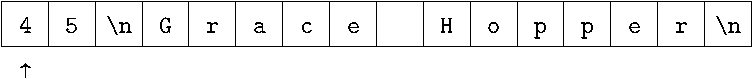
\includegraphics{figs/hopper1.pdf}
\caption{A stream of characters as seen by a \java{Scanner}.}
\label{fig.hopper1}
\end{center}
\end{figure}

%TODO define call/invoke or use other term?

The arrow indicates the next character to be read by \java{Scanner}.
When you call \java{nextInt}, it reads characters until it gets to a non-digit.
Figure~\ref{fig.hopper2} shows the state of the stream after \java{nextInt} is called.

\begin{figure}[!ht]
\begin{center}
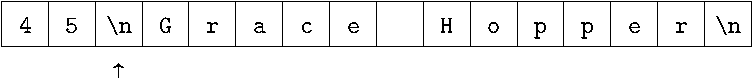
\includegraphics{figs/hopper2.pdf}
\caption{A stream of characters after \java{nextInt} is called.}
\label{fig.hopper2}
\end{center}
\end{figure}

At this point, \java{nextInt} returns \java{45}.
The program then displays the prompt \java{"What is your name? "} and calls \java{nextLine}, which reads characters until it gets to a newline.
But since the next character is already a newline, \java{nextLine} returns the empty string \java{""}.

To solve this problem, you need an extra \java{nextLine} after \java{nextInt}.

\begin{code}
System.out.print("What is your age? ");
age = in.nextInt();
in.nextLine();  // read the newline
System.out.print("What is your name? ");
name = in.nextLine();
System.out.printf("Hello %s, age %d\n", name, age);
\end{code}

This technique is common when reading \java{int} or \java{double} values that appear on their own line.
First you read the number, and then you read the rest of the line, which is just a newline character.


% DW suggests we also cover PrintWriter to write files --
% add an appendix on File I/O since it involves try/catch?

\section{Vocabulary}

\begin{description}

\term{package}
A directory of classes that are related to each other.
%Java classes are organized into packages.

\term{address}
The location of a value in computer memory, often represented as a hexadecimal integer.

\term{library}
A collection of packages and classes that are available for use in other programs.
%Libraries are often distributed in {\tt .jar} (Java Archive) files.

%\term{abstraction}
%The process of reducing information and/or detail to focus on high-level concepts.

%\term{operating system}
%Software that is always running behind the scenes on your computer.
%It controls the execution of application programs and manages hardware resources.

%\term{byte}
%A single unit of data on a computer; enough to represent one character.

%\term{utility class}
%A class that provides commonly needed functionality.

\term{import statement}
A statement that allows programs to use classes defined in other packages.

\term{token}
The smallest unit of source code, such as an individual word, literal value, or symbol.

%\term{syntax}
%The structure of a program; the arrangement of the words and symbols it contains.

%\term{semantics}
%The meaning of a program; the low-level instructions it should perform.

\term{literal}
A value that appears in source code.
For example, \java{"Hello"} is a string literal, and \java{74} is an integer literal.

\term{prompt}
A brief message displayed in a print statement that asks the user for input.

\term{magic number}
A number that appears without explanation as part of an expression.
It should generally be replaced with a constant.

\term{constant}
A variable, declared as \java{final}, whose value cannot be changed.

\term{format string}
The string in \java{System.out.printf} that specifies the format of the output.

\term{format specifier}
A special code that begins with a percent sign and specifies the data type and format of the corresponding value.

\term{type cast}
An operation that explicitly converts one data type into another.
In Java it appears as a type name in parentheses, like \java{(int)}.

%\term{truncate}
%To make shorter by cutting something off.
%Casting a floating-point value to an integer simply removes the fractional part.

\term{modulo}
An operation that yields the remainder when one integer is divided by another.
In Java, it is denoted with a percent sign: \java{5 \% 2} is \java{1}.

\term{modulus}
The value of \java{b} in the expression \java{a \% b}.
It often represents unit conversions, such as 24 hours in a day, 60 minutes in an hour, etc.

\end{description}


\section{Exercises}

The code for this chapter is in the {\tt ch03} directory of {\tt ThinkJavaCode2}.
See page~\pageref{code} for instructions on how to download the repository.
Before you start the exercises, we recommend that you compile and run the examples.

If you have not already read Appendix~\ref{commandline}, now might be a good time.
It describes the command-line interface, which is a powerful and efficient way to interact with your computer.


\begin{exercise}  %%V6 Ex3.1

When you use \java{printf}, the Java compiler does not check your format string.
See what happens if you try to display a value with type \java{int} using \java{\%f}.
And what happens if you display a \java{double} using \java{\%d}?
What if you use two format specifiers, but then only provide one value?

\end{exercise}

%If you try to print an integer with \java{\%f} or a floating-point number using \java{\%d}, you get an \java{IllegalFormatConversionException}.


\begin{exercise}  %%V6 Ex3.2

Write a program that converts a temperature from Celsius to Fahrenheit.
It should (1) prompt the user for input, (2) read a \java{double} value from the keyboard, (3) calculate the result, and (4) format the output to one decimal place.
For example, it should display {\tt "24.0 C = 75.2 F"}.

Here is the formula.
Be careful not to use integer division!
%
\[ F = C \times \frac{9}{5} + 32 \]

\end{exercise}


\begin{exercise}  %%V6 Ex3.3

Write a program that converts a total number of seconds to hours, minutes, and seconds.
It should (1) prompt the user for input, (2) read an integer from the keyboard, (3) calculate the result, and (4) use \java{printf} to display the output.
For example, {\tt "5000 seconds = 1 hours, 23 minutes, and 20 seconds"}.

{\it Hint:} Use the remainder operator.

\end{exercise}


\begin{exercise}  %%V6 Ex3.4
\label{guess}

The goal of this exercise is to program a ``Guess My Number'' game.
When it's finished, it will work like this:

\begin{stdout}
I'm thinking of a number between 1 and 100
(including both). Can you guess what it is?
Type a number: 45
Your guess is: 45
The number I was thinking of is: 14
You were off by: 31
\end{stdout}

To choose a random number, you can use the \java{Random} class in \java{java.util}.
Here's how it works:

\index{GuessStarter.java}

\begin{trinket}{GuessStarter.java}
import java.util.Random;

public class GuessStarter {

    public static void main(String[] args) {
        // pick a random number
        Random random = new Random();
        int number = random.nextInt(100) + 1;
        System.out.println(number);
    }
}
\end{trinket}

\index{new}
\index{operator!new}

Like the \java{Scanner} class we saw in this chapter, \java{Random} has to be imported before we can use it.
And as we saw with \java{Scanner}, we have to use the \java{new} operator to create a \java{Random} (number generator).

Then we can use the method \java{nextInt} to generate a random number.
In this example, the result of \java{nextInt(100)} will be between 0 and 99, including both.
Adding 1 yields a number between 1 and 100, including both.

\begin{enumerate}

\item The definition of \java{GuessStarter} is in a file called {\tt GuessStarter.java}, in the directory called {\tt ch03}, in the repository for this book.
%Instructions for downloading this code are on page~\pageref{code}.

\item Compile and run this program.

\item Modify the program to prompt the user, then use a \java{Scanner} to read a line of user input.
Compile and test the program.

\item Read the user input as an integer and display the result.
Again, compile and test.

\item Compute and display the difference between the user's guess and the number that was generated.

\end{enumerate}

\end{exercise}


\chapter{Conditionals and logic}

\index{boolean}
\index{type!boolean}

The programs we've seen in previous chapters do pretty much the same thing every time, regardless of the input.
For more complex computations, programs usually react to inputs, check for certain conditions, and generate applicable results.
This chapter introduces Java language features for expressing logic and making decisions.
We'll also take a look at the \java{Math} class, which provides methods for common mathematical operations.


\section{Relational operators}

\index{operator!relational}
\index{relational operator}
\index{comparison operator}

Java has six {\bf relational operators} that test the relationship between two values (e.g., whether they are equal, or whether one is greater than the other).
The following expressions show how they are used:

\begin{code}
x == y          // x is equal to y
x != y          // x is not equal to y
x > y           // x is greater than y
x < y           // x is less than y
x >= y          // x is greater than or equal to y
x <= y          // x is less than or equal to y
\end{code}

\index{Boole, George}

The result of a relational operator is one of two special values: \java{true} or \java{false}.
These values belong to the data type \java{boolean}, named after the mathematician George Boole.
He developed an algebraic way of representing logic.

\index{assignment}
\index{operator!assignment}
\index{== equals operator}

You are probably familiar with these operators, but notice how Java is different from mathematical symbols like $=$, $\neq$, and $\geq$.
A common error is to use a single \java{=} instead of a double \java{==} when comparing values.
Remember that \java{=} is the {\em assignment} operator, and \java{==} is a {\em relational} operator.
In addition, the operators \java{=<} and \java{=>} do not exist.

The two sides of a relational operator have to be compatible.
For example, the expression \java{5 < "6"} is invalid because \java{5} is an \java{int} and \java{"6"} is a \java{String}.
When comparing values of different numeric types, Java applies the same conversion rules we saw previously with the assignment operator.
For example, when evaluating the expression \java{5 < 6.0}, Java automatically converts the \java{5} to \java{5.0}.

%Most relational operators don't work with strings.
%But confusingly, \java{==} and \java{!=} do work with strings -- they just don't do what you expect.
%We'll explain what they do later; in the meantime, don't use them with strings.
%Instead, you should use the \java{equals} method:
%
%\begin{code}
%String fruit1 = "Apple";
%String fruit2 = "Orange";
%System.out.println(fruit1.equals(fruit2));
%\end{code}
%
%The result of \java{fruit1.equals(fruit2)} is the boolean value \java{false}.


\section{The if-else statement}

\index{conditional statement}
\index{statement!conditional}
\index{if statement}
\index{statement!if}

To write useful programs, we almost always need to check conditions and react accordingly.
{\bf Conditional statements} give us this ability.
The simplest conditional statement in Java is the \java{if} statement:

\begin{code}
if (x > 0) {
    System.out.println("x is positive");
}
\end{code}

\index{block}

The expression in parentheses is called the condition.
If it is true, the statements in braces get executed.
If the condition is false, execution skips over that {\bf block} of code.
The condition in parentheses can be any \java{boolean} expression.

\index{branch}
\index{statement!else}

A second form of conditional statement has two possibilities, indicated by \java{if} and \java{else}.
The possibilities are called {\bf branches}, and the condition determines which one gets executed:

\begin{code}
if (x % 2 == 0) {
    System.out.println("x is even");
} else {
    System.out.println("x is odd");
}
\end{code}

If the remainder when \java{x} is divided by 2 is zero, we know that \java{x} is even, and the program displays a message to that effect.
If the condition is false, the second print statement is executed instead.
Since the condition must be true or false, exactly one of the branches will run.

The braces are optional for branches that have only one statement.
So we could have written the previous example this way:

\begin{code}
if (x % 2 == 0)
    System.out.println("x is even");
else
    System.out.println("x is odd");
\end{code}

However, it's better to use braces -- even when they are optional -- to avoid making the mistake of adding statements to an \java{if} or \java{else} block and forgetting to add the braces.
This code is misleading because it's not indented correctly:

\begin{code}
if (x > 0)
    System.out.println("x is positive");
    System.out.println("x is not zero");
\end{code}

Since there are no braces, only the first \java{println} is part of the \java{if} statement.
Here is what the compiler actually sees:

\begin{code}
if (x > 0) {
    System.out.println("x is positive");
}
    System.out.println("x is not zero");
\end{code}

As a result, the second \java{println} runs no matter what.
Even experienced programmers make this mistake; search the web for Apple's ``goto fail'' bug.

\index{\{\} curly braces}

In all previous examples, notice how there is no semicolon at the end of the \java{if} or \java{else} lines.
Instead, a new block should be defined using curly braces.
Another common mistake is to put a semicolon after the condition, like this:

\begin{code}
int x = 1;
if (x % 2 == 0); {  // incorrect semicolon
    System.out.println("x is even");
}
\end{code}

This code will compile, but the program will output \java{"x is even"} regardless what value \java{x} is.
Here is the same incorrect code with better formatting:

\begin{code}
int x = 1;
if (x % 2 == 0)
    ;  // empty statement
{
    System.out.println("x is even");
}
\end{code}

Because of the semicolon, the \java{if} statement compiles as if there are no braces, and the subsequent block runs independently.
As a general rule, each line of Java code should end with a semicolon or brace -- but not both.

The compiler won't complain if you omit optional braces or write empty statements.
Doing so is allowed by the Java language, but it often results in bugs that are difficult to find.
Development tools like Checkstyle (see Appendix~\ref{checkstyle}) can warn you about these and other kinds of programming mistakes.


\section{Chaining and nesting}

\index{chaining}

Sometimes you want to check related conditions and choose one of several actions.
One way to do this is by {\bf chaining} a series of \java{if} and \java{else} blocks:

\begin{code}
if (x > 0) {
    System.out.println("x is positive");
} else if (x < 0) {
    System.out.println("x is negative");
} else {
    System.out.println("x is zero");
}
\end{code}

These chains can be as long as you want, although they can be difficult to read if they get out of hand.
One way to make them easier to read is to use standard indentation, as demonstrated in these examples.
If you keep all the statements and braces lined up, you are less likely to make syntax errors.

Notice that the last branch is simply \java{else}, not \java{else if (x == 0)}.
At this point in the chain, we know that \java{x} is not positive and \java{x} is not negative.
There is no need to test whether \java{x} is zero, because there is no other possibility.

\index{nesting}

In addition to chaining, you can also make complex decisions by {\bf nesting} one conditional statement inside another.
We could have written the previous example as:

\begin{code}
if (x > 0) {
    System.out.println("x is positive");
} else {
    if (x < 0) {
        System.out.println("x is negative");
    } else {
        System.out.println("x is zero");
    }
}
\end{code}

The outer conditional has two branches.
The first branch contains a \java{print} statement, and the second branch contains another conditional statement, which has two branches of its own.
These two branches are also \java{print} statements, but they could have been conditional statements as well.

\index{nested!conditions}

These kinds of nested structures are common, but they can become difficult to read very quickly.
Good indentation is essential to make the structure (or intended structure) apparent to the reader.


\section{Logical operators}

\index{logical operator}
\index{operator!logical}
\index{and operator}
\index{or operator}
\index{not operator}

In addition to the relational operators, Java also has three {\bf logical operators}: \java{&&}, \java{||}, and \java{!}, which respectively stand for {\em and}, {\em or}, and {\em not}.
The results of these operators are similar to their meanings in English.

For example, \java{x > 0 && x < 10} is true when \java{x} is both greater than zero {\em and} less than 10.
The expression \java{evenFlag || n \% 3 == 0} is true if either condition is true, that is, if \java{evenFlag} is true {\em or} the number \java{n} is divisible by 3.
Finally, the \java{!} operator inverts a boolean expression.
So \java{!evenFlag} is true if \java{evenFlag} is false.

In order for an expression with \java{&&} to be true, both sides of the \java{&&} operator must be true.
And in order for an expression with \java{||} to be false, both sides of the \java{||} operator must be false.

The \java{&&} operator can be used to simplify nested \java{if} statements.
For example, following code can be rewritten with a single condition.

\begin{code}
if (x == 0) {
    if (y == 0) {
        System.out.println("Both x and y are zero");
    }
}
\end{code}

\begin{code}
// combined
if (x == 0 && y == 0) {
    System.out.println("Both x and y are zero");
}
\end{code}

Likewise, the \java{||} operator can simplify chained \java{if} statements.
Since the branches are the same, there is no need to duplicate that code.

\begin{code}
if (x == 0) {
    System.out.println("Either x or y is zero");
} else if (y == 0) {
    System.out.println("Either x or y is zero");
}
\end{code}

\begin{code}
// combined
if (x == 0 || y == 0) {
    System.out.println("Either x or y is zero");
}
\end{code}

Of course if the statements in the branches were different, we could not combine them into one block.
But it's useful to explore different ways of representing the same logic, especially when it's complex.

\index{short circuit}

Logical operators evaluate the second expression only when necessary.
For example, \java{true || anything} is always true, so Java does not need to evaluate the expression \java{anything}.
Likewise, \java{false && anything} is always false.

Ignoring the second operand, when possible, is called {\bf short circuit} evaluation, by analogy with an electrical circuit.
Short circuit evaluation can save time, especially if \java{anything} takes a long time to evaluate.
It can also avoid unnecessary errors, if \java{anything} might fail.


\section{De Morgan's laws}

Sometimes you need to negate an expression containing a mix of relational and logical operators.
For example, to test if \java{x} and \java{y} are both nonzero, you could write:

\begin{code}
if (!(x == 0 || y == 0)) {
    System.out.println("Neither x nor y is zero");
}
\end{code}

\index{De Morgan's laws}

This condition is difficult to read because of the \java{!} and parentheses.
A better way to negate logic expressions is to apply {\bf De Morgan's laws}:

\begin{itemize}
\item \java{!(A && B)} ~is the same as~ \java{!A || !B}
\item \java{!(A || B)} ~is the same as~ \java{!A && !B}
\end{itemize}

Negating a logical expression is the same as negating each term and changing the operator.
The \java{!} operator takes precedence over \java{&&} and \java{||}, so you don't have to put parentheses around the individual terms \java{!A} and \java{!B}.

De Morgan's laws also apply to the relational operators.
In this case, negating each term means using the ``opposite'' relational operator.

\begin{itemize}
\item \java{!(x < 5 && y == 3)} ~is the same as~ \java{x >= 5 || y != 3}
\item \java{!(x >= 1 || y != 7)} ~is the same as~ \java{x < 1 && y == 7}
\end{itemize}

It may help to read these examples out loud in English.
For instance, ``If I don't want the case where $x$ is less than 5 and $y$ is 3, then I need $x$ to be greater than or equal to 5, or I need $y$ to be anything but 3.''

Returning to the previous example, here is the revised condition.
In English, it reads ``if $x$ is not zero and $y$ is not zero.''
The logic is the same, and the source code is easier to read.

\begin{code}
if (x != 0 && y != 0) {
    System.out.println("Neither x nor y is zero");
}
\end{code}


\section{Boolean variables}

\index{expression}
\index{type!boolean}

To store a \java{true} or \java{false} value, you need a \java{boolean} variable.
You can declare and assign them like other variables.
In this example, the first line is a variable declaration, the second is an assignment, and the third is both:

\begin{code}
boolean flag;
flag = true;
boolean testResult = false;
\end{code}

\index{initialize}
\index{statement!initialization}

Since relational and logical operators evaluate to a \java{boolean} value, you can store the result of a comparison in a variable:

\begin{code}
boolean evenFlag = (n % 2 == 0);    // true if n is even
boolean positiveFlag = (x > 0);     // true if x is positive
\end{code}

\index{flag}

The parentheses are unnecessary, but they make the code easier to understand.
A variable defined in this way is called a {\bf flag}, because it signals or ``flags'' the presence or absence of a condition.

You can use flag variables as part of a conditional statement:

\begin{code}
if (evenFlag) {
    System.out.println("n was even when I checked it");
}
\end{code}

Flags may not seem that useful at this point, but they will help simplify complex conditions later on.
Each part of a condition can be stored in a separate flag, and these flags can be combined with logical operators.

Notice that you don't have to write ~\java{if (evenFlag == true)}.
Since \java{evenFlag} is a \java{boolean}, it's already a condition.
Furthermore, to check if a flag is \java{false}:

\begin{code}
if (!evenFlag) {
    System.out.println("n was odd when I checked it");
}
\end{code}


\section{Math methods}

In the next two sections, we'll take a break from conditions and logic and discuss other areas of mathematics in Java.

\index{Math class}
\index{class!Math}

The Java library includes a \java{Math} class that provides common mathematical operations.
\java{Math} is in the \java{java.lang} package, so you don't have to import it.

\begin{code}
double root = Math.sqrt(17.0);
double angle = 1.5;
double height = Math.sin(angle);
\end{code}

The first line sets \java{root} to the square root of 17.
The third line finds the sine of 1.5 (the value of \java{angle}).

\index{degrees}
\index{radians}
\index{pi}

Values for the trigonometric functions -- \java{sin}, \java{cos}, and \java{tan} -- must be in {\em radians}.
To convert from degrees to radians, you can divide by 180 and multiply by $\pi$.
Conveniently, the \java{Math} class provides a constant double named \java{PI} that contains an approximation of $\pi$:

\begin{code}
double degrees = 90;
double angle = degrees / 180.0 * Math.PI;
\end{code}

Notice that \java{PI} is in capital letters.
Java does not recognize \java{Pi}, \java{pi}, or \java{pie}.
Also, \java{PI} is the name of a variable, not a method, so it doesn't have parentheses.
The same is true for the constant \java{Math.E}, which approximates Euler's number.

Converting to and from radians is a common operation, so the \java{Math} class provides methods that do that for you.

\begin{code}
double radians = Math.toRadians(180.0);
double degrees = Math.toDegrees(Math.PI);
\end{code}

\index{long}
\index{type!long}

Another useful method is \java{round}, which rounds a floating-point value to the nearest integer and returns a \java{long}.
The following result is 63 (rounded up from 62.8319).

\begin{code}
long x = Math.round(Math.PI * 20.0);
\end{code}

A \java{long} is like an \java{int}, but bigger.
More specifically, an \java{int} uses 32 bits of memory; the largest value it can hold is $2^{31}-1$, which is about 2 billion.
A \java{long} uses 64 bits, so the largest value is $2^{63}-1$, which is about 9 quintillion.

Take a minute to read the documentation for these and other methods in the \java{Math} class.
The easiest way to find documentation for Java classes is to do a web search for ``Java'' and the name of the class.


\section{Composition}

\index{expression}
\index{argument}

You have probably learned to evaluate simple expressions like $\sin(\pi/2)$ and $\log(1/x)$.
First, you evaluate the expression in parentheses, which is called the {\bf argument} of the function.
Then you can evaluate the function itself, either by hand or by punching it into a calculator.

This process can be applied repeatedly to evaluate more complex expressions like $\log(1/\sin(\pi/2))$.
First we evaluate the argument of the innermost function ($\pi/2 = 1.57$), then evaluate the function itself ($\sin(1.57) = 1.0$), and so on.

\index{composition}
\index{expression}

Just as with mathematical functions, Java methods can be {\bf composed} to solve complex problems.
That means you can use one method as part of another.
In fact, you can use any expression as an argument to a method, as long as the resulting value has the correct type:

\begin{code}
double x = Math.cos(angle + Math.PI / 2.0);
\end{code}

This statement divides \java{Math.PI} by two, adds the result to \java{angle}, and computes the cosine of the sum.
You can also take the result of one method and pass it as an argument to another:

\begin{code}
double x = Math.exp(Math.log(10.0));
\end{code}

In Java, the \java{log} method always uses base $e$.
So this statement finds the log base $e$ of 10, and then raises $e$ to that power.
The result gets assigned to \java{x}.

Some math methods take more than one argument.
For example, \java{Math.pow} takes two arguments and raises the first to the power of the second.
This line computes $2^{10}$ and assigns the value \java{1024.0} to the variable \java{x}:

\begin{code}
double x = Math.pow(2.0, 10.0);
\end{code}

When using \java{Math} methods, beginners often forget the word \java{Math}.
For example, if you just write \java{x = pow(2.0, 10.0)}, you will get a compiler error:

\begin{stdout}
File: Test.java  [line: 5]
Error: cannot find symbol
  symbol:   method pow(double,double)
  location: class Test
\end{stdout}

The message ``cannot find symbol'' is confusing, but the last two lines provide a useful hint.
The compiler is looking for a method named \java{pow} in the file \java{Test.java} (the file for this example).
If you don't specify a class name when referring to a method, the compiler looks in the current class by default.


\section{Validating input}
\label{validate}

\index{validate}
\index{hacker}

One of the most important tasks in any computer program is to {\bf validate} input from the user.
People often make mistakes while typing, especially on smartphones, and incorrect inputs may cause your program to fail.
Even worse, someone (i.e., a {\bf hacker}) may intentionally try to break into your system by entering unexpected inputs.

Consider this simple program that prompts the user for a number and computes its logarithm:

\begin{code}
Scanner in = new Scanner(System.in);
System.out.print("Enter a number: ");
double x = in.nextDouble();
double y = Math.log(x);
System.out.println("The log is " + y);
\end{code}

In mathematics, the natural logarithm (base $e$) is undefined when $x < 0$.
If you ask for \java{Math.log(-1)}, it will return {\bf NaN} which stands for ``not a number''.
Many users are confused when they see NaN; it often looks like a bug.
We can use an \java{if} statement to make the output more user friendly.

\begin{code}
if (x >= 0) {
    double y = Math.log(x);
    System.out.println("The log is " + y);
} else {
    System.out.println("The log is undefined");
}
\end{code}

The output is better now, but there is another problem.
What if the user doesn't enter a number at all?
What would happen if they typed the word ``hello'', either on accident or on purpose?

\index{InputMismatchException}
\index{exception!InputMismatch}

\begin{small}
\begin{stdout}
Exception in thread "main" java.util.InputMismatchException
    at java.util.Scanner.throwFor(Scanner.java:864)
    at java.util.Scanner.next(Scanner.java:1485)
    at java.util.Scanner.nextDouble(Scanner.java:2413)
    at Logarithm.main(Logarithm.java:8)
\end{stdout}
\end{small}

\index{run-time error}
\index{testing}

If the user inputs a \java{String} when we expect a \java{double}, Java reports an ``input mismatch'' exception.
We can prevent this run-time error from happening by testing the input first.

The \java{Scanner} class provides \java{hasNextDouble}, which checks whether the next input can be interpreted as a \java{double}.
If not, we can display an error message.

\begin{code}
if (!in.hasNextDouble()) {
    String word = in.next();
    System.err.println(word + "is not a number");
    return;
}
\end{code}

\index{next!Scanner}

In contrast to \java{in.nextLine}, which returns an entire line of input, the \java{in.next} method returns only the next token of input.
We can use \java{in.next} to show the user exactly which word they typed was not a number.

\index{System.err}

This example also uses \java{System.err}, which is an \java{OutputStream} for error messages and warnings.
Some development environments display output to \java{System.err} with a different color or in a separate window.

\index{return}
\index{statement!return}

The \java{return} statement allows you to exit a method before you reach the end of it.
Returning from \java{main} terminates the program.

Notice the use of the \java{!} operator before \java{in.hasNextDouble()}, instead of testing the condition \java{in.hasNextDouble() == false}.
Since \java{hasNextDouble} returns a boolean, it is already a condition.


\section{Example program}

In this chapter we have seen relational and logical operators, \java{if} statements, the \java{Math} class, and validating input.
The following program shows how the individual code examples in the last section fit together.

\index{Logarithm.java}

\begin{trinket}{Logarithm.java}
import java.util.Scanner;

/**
 * Demonstrates input validation using if statements.
 */
public class Logarithm {

    public static void main(String[] args) {

        // prompt for input
        Scanner in = new Scanner(System.in);
        System.out.print("Enter a number: ");

        // check the format
        if (!in.hasNextDouble()) {
            String word = in.next();
            System.err.println(word + " is not a number");
            return;
        }

        // check the range
        double x = in.nextDouble();
        if (x >= 0) {
            double y = Math.log(x);
            System.out.println("The log is " + y);
        } else {
            System.out.println("The log is undefined");
        }
    }
}
\end{trinket}

What started as five lines of code at the beginning of Section~\ref{validate} is now a 30-line program.
Making programs robust (and secure) often requires a lot of additional checking, as shown in this example.

\index{comment}

It's important to write comments every few lines to make your code easier to understand.
Comments not only help other people read your code, they also help you document what you're trying to do.
If there's a mistake the code, it's a lot easier to find when there are good comments.


\section{Vocabulary}

\begin{description}

\term{boolean}
A data type with only two possible values, \java{true} and \java{false}.

\term{relational operator}
An operator that compares two values and produces a \java{boolean} indicating the relationship between them.

\term{conditional statement}
A statement that uses a condition to determine which statements to execute.

\term{block}
A sequence of statements, surrounded by braces, that generally runs as the result of a condition.

\term{branch}
One of the alternative blocks after a conditional statement.
For example, an \java{if}-\java{else} statement has two branches.

\term{chaining}
A way of joining several conditional statements in sequence.

\term{nesting}
Putting a conditional statement inside one or both branches of another conditional statement.

\term{logical operator}
An operator that combines boolean values and produces a boolean value.

\term{short circuit}
A way of evaluating logical operators that only evaluates the second operand if necessary.

\term{De Morgan's laws}
Mathematical rules that show how to negate a logical expression.

\term{flag}
A variable (usually \java{boolean}) that represents a condition or status.

\term{argument}
A value that you provide when you call a method.
This value must have the type that the method expects.

\term{composition}
The ability to combine simple expressions and statements into compound expressions and statements.

\term{validate}
To confirm that an input value is of the correct type and within the expected range.

\term{hacker}
A programmer who breaks into computer systems.
The term hacker may also apply to someone who enjoys writing code.

\term{NaN}
A special floating-point value that stands for ``not a number''.

\end{description}


\section{Exercises}

The code for this chapter is in the {\tt ch04} directory of {\tt ThinkJavaCode2}.
See page~\pageref{code} for instructions on how to download the repository.
Before you start the exercises, we recommend that you compile and run the examples.

If you have not already read Appendix~\ref{cltesting}, now might be a good time.
It describes an efficient way to test programs that take input from the user and display specific output.


\begin{exercise}  %%V6.5 NEW

Using the following variables, evaluate the logic expressions in the table below.
Write your answers as true, false, or error.

\begin{code}
boolean yes = true;
boolean no = false;
int loVal = -999;
int hiVal = 999;
double grade = 87.5;
double amount = 50.0;
String hello = "world";
\end{code}

\vspace{1ex}

\begin{center}
\begin{tabular}{|l|l|}
\hline
Expression & Result \\
\hline
\hline
\java{yes == no || grade > amount} & \hspace{5em} \\
\hline
\java{amount == 40.0 || 50.0} &  \\
\hline
\java{hiVal != loVal || loVal < 0} &  \\
\hline
\java{True || hello.length() > 0} &  \\
\hline
\java{hello.isEmpty() && yes} &  \\
\hline
\java{grade <= 100 && !false} &  \\
\hline
\java{!yes || no} &  \\
\hline
\java{grade > 75 > amount} &  \\
\hline
\java{amount <= hiVal && amount >= loVal} &  \\
\hline
\java{no && !no || yes && !yes} &  \\
\hline
\end{tabular}
\end{center}

\end{exercise}


\begin{exercise}  %%V6 Ex5.1

Rewrite the following code using a single \java{if} statement.

\begin{code}
if (x > 0) {
    if (x < 10) {
        System.out.println("positive single digit number.");
    }
}
\end{code}

\end{exercise}


\begin{exercise}  %%V6 Ex5.4

Fermat's Last Theorem says that there are no integers $a$, $b$, and $c$ such that $a^n + b^n = c^n$, except when $n \leq 2$.

Write a program named \java{Fermat.java} that inputs four integers (\java{a}, \java{b}, \java{c}, and \java{n}) and checks to see if Fermat's theorem holds.
If $n$ is greater than 2 and $a^n + b^n = c^n$, the program should display ``Holy smokes, Fermat was wrong!''
Otherwise the program should display ``No, that doesn't work.''

{\it Hint:} You may want to use \java{Math.pow}.

\end{exercise}


\begin{exercise}  %%V6 Ex5.7

Now that we have conditional statements, we can get back to the ``Guess My Number'' game from Exercise~\ref{guess}.

You should already have a program that chooses a random number, prompts the user to guess it, and displays the difference between the guess and the chosen number.

Adding a small amount of code at a time, and testing as you go, modify the program so it tells the user whether the guess is too high or too low, and then prompts the user for another guess.

The program should continue until the user gets it right or guesses incorrectly three times.
If the user guesses the correct number, display a message and terminate the program.

\end{exercise}


\begin{exercise}  %%V6.5 NEW

Write a program named \java{Quadratic.java} that finds the roots of $ax^2 + bx + c = 0$ using the quadratic formula:
$$ x = \frac{-b \pm \sqrt{b^2 - 4ac}}{2a} $$
Prompt the user to input integers for $a$, $b$, and $c$.
Compute the two solutions for $x$, and display the results.

Your program should be able to handle inputs for which there is only one or no solution.
Specifically, it should not divide by zero or take the square root of a negative number.

Be sure to validate all inputs.
The user should never see an input mismatch exception.
Display specific error messages that include the invalid input.

\end{exercise}


\begin{exercise}  %%V6 Ex6.3

If you are given three sticks, you may or may not be able to arrange them in a triangle.
For example, if one of the sticks is 12 inches long and the other two are one inch long, you will not be able to get the short sticks to meet in the middle.
For any three lengths, there is a simple test to see if it is possible to form a triangle:

\begin{quotation}
\noindent
If any of the three lengths is greater than the sum of the other two, you cannot form a triangle.
\end{quotation}

Write a program named \java{Triangle.java} that inputs three integers, and then outputs whether you can (or cannot) form a triangle from the given lengths.
%The point of this exercise is to use conditional statements to write a value method.
Reuse your code from the previous exercise to validate the inputs.
Display an error if any of the lengths are negative or zero.

\end{exercise}


\chapter{Methods and testing}

So far we've written programs that have only one method (\java{main}).
In this chapter, we'll show you how to organize programs into multiple methods.
We'll also learn how to trace the order in which a program runs.
Finally, we'll discuss strategies for incrementally developing and testing your code.

%At a conceptual level, a method represents a mathematical {\em function} or a general {\em procedure}.
%Regardless whether they return a value or not, methods enable you to break down a complex program into smaller units of code.


\section{Defining new methods}
\label{adding_methods}

\index{method!declaration}

%You have probably guessed by now that you can define more than one method in a class.

Some methods perform a computation and return a result.
For example, \java{Math.sqrt(25)} returns the value \java{5.0}.
Other methods (including \java{main}) carry out a sequence of actions, without returning a result.
Java uses the keyword \java{void} to define such methods.
Here's a simple example:

\index{NewLine.java}

\begin{trinket}[310]{NewLine.java}
public class NewLine {

    public static void newLine() {
        System.out.println();
    }

    public static void main(String[] args) {
        System.out.println("First line.");
        newLine();
        System.out.println("Second line.");
    }
}
\end{trinket}

\index{main}
\index{case-sensitive}

The name of the class is \java{NewLine}.
By convention, class names begin with a capital letter.
\java{NewLine} contains two methods, \java{newLine} and \java{main}.
Remember that Java is case-sensitive, so \java{NewLine} and \java{newLine} are not the same.

\index{camel case}

Method names should begin with a lowercase letter and use ``camel case'', which is a cute name for \java{jammingWordsTogetherLikeThis}.
You can use any name you want for methods, except \java{main} or any of the Java keywords.

\index{public}
\index{invoke}
\index{void}
\index{type!void}

\java{newLine} and \java{main} are \java{public}, which means they can be {\bf invoked} (or called) from other classes.
%They are both \java{static}, but we won't yet explain what that means.
And they are both \java{void}, which means that they don't return a result (unlike the \java{Math} methods, for example).

The output of this program is:

\begin{stdout}
First line.

Second line.
\end{stdout}

Notice the extra space between the lines.
If we wanted more space between them, we could invoke the same method repeatedly.

%Or we could write yet another method (named \java{threeLine}) that displays three blank lines:
%Pulling together the code from the previous section, the complete program looks like this:

\begin{trinket}{NewLine.java}
public class NewLine {

    public static void newLine() {
        System.out.println();
    }

    public static void threeLine() {
        newLine();
        newLine();
        newLine();
    }

    public static void main(String[] args) {
        System.out.println("First line.");
        threeLine();
        System.out.println("Second line.");
    }
}
\end{trinket}

In this example, \java{main} invokes \java{threeLine}, and \java{threeLine} invokes \java{newLine} three times.
%Since \java{newLine} has no parameters, it requires no arguments, as shown when it is invoked in \java{main}.
Because \java{newLine} is in the same class as \java{threeLine}, we don't have to specify the class name like \java{NewLine.newLine()}.

Beginners wonder why it's worth the trouble to write other methods, when they could just do everything in \java{main}.
The \java{NewLine} example demonstrates a few reasons:

\begin{itemize}

\item Creating a new method allows you to {\em name a block of statements}, which makes the code easier to read and understand.
%Methods simplify a program by hiding complex computations behind a single statement, and by using English words in place of arcane code.
%Which is clearer, \java{newLine} or \java{System.out.println()}?

\item Introducing new methods can {\em make the program shorter} by eliminating repetitive code.
For example, to display nine consecutive newlines, you could invoke \java{threeLine} three times.

\item A common problem-solving technique is to {\em break problems down} into sub-problems.
Methods allow you to focus on each sub-problem in isolation, and then compose them into a complete solution.

\end{itemize}

Perhaps most importantly, organizing your code into multiple methods allows you to test individual parts of your program separately.
It's easier to get a complex program working if you know that each method works correctly.


\section{Flow of execution}

\index{flow of execution}

When you look at a class definition that contains several methods, it is tempting to read it from top to bottom.
But that is {\em not} the {\bf flow of execution}, or the order the program actually runs.
The \java{NewLine} program runs methods in the opposite order than they are listed.

Programs always begin at the first statement of \java{main}, regardless of where it is in the source file.
Statements are executed one at a time, in order, until you reach a method invocation, which you can think of as a detour.
Instead of going to the next statement, you jump to the first line of the invoked method, execute all the statements there, and then come back and pick up exactly where you left off.

That sounds simple enough, but remember that one method can invoke another one.
In the middle of \java{main}, the previous example goes off to execute the statements in \java{threeLine}.
While in \java{threeLine}, it goes off to execute \java{newLine}.
Then \java{newLine} invokes \java{println}, which causes yet another detour.

Fortunately, Java is good at keeping track of which methods are running.
So when \java{println} completes, it picks up where it left off in \java{newLine}; when \java{newLine} completes, it goes back to \java{threeLine}; and when \java{threeLine} completes, it gets back to \java{main}.

%In summary, when you read a program, don't read from top to bottom.
%Instead, follow the flow of execution.

%Technically, the program does not terminate at the end of \java{main}.
%Instead, execution picks up where it left off in the program that invoked \java{main}, which is the Java interpreter.
%The interpreter takes care of things like deleting windows and general cleanup, and {\em then} the program terminates.


\section{Parameters and arguments}

Some of the methods we have used require arguments, which are the values you provide in parentheses when you invoke the method.

For example, the \java{Math.sin} method takes a \java{double} argument.
To find the sine of a number, you have to provide the number: \java{Math.sin(0.0)}.
Similarly, the \java{System.out.println} method takes a \java{String} argument.
To display a message, you have to provide the message: \java{System.out.println("Hello")}.

\index{parameter}
\index{argument}

When you invoke a method, you provide the arguments.
When you define a method, you name the {\bf parameters}, which are variables that indicate what arguments are required.
The following class shows an example:

\index{PrintTwice.java}

\begin{trinket}[295]{PrintTwice.java}
public class PrintTwice {

    public static void printTwice(String s) {
        System.out.println(s);
        System.out.println(s);
    }

    public static void main(String[] args) {
        printTwice("Don't make me say this twice!");
    }
}
\end{trinket}

The \java{printTwice} method has a parameter named \java{s} with type \java{String}.
When you invoke \java{printTwice}, you have to provide an argument with type \java{String}.

%\java{main} has a single parameter, called \java{args}, which has type \java{String[]}.
%That means that whoever invokes \java{main} must provide an array of strings (we'll get to arrays in a later chapter).

Before the method executes, the argument gets assigned to the parameter.
In this example, the argument \java{"Don't make me say this twice!"} gets assigned to the parameter \java{s}.

\index{parameter passing}

This process is called {\bf parameter passing} because the value gets passed from outside the method to the inside.
An argument can be any kind of expression, so if you have a \java{String} variable, you can use its value as an argument:

\begin{code}
String message = "Never say never.";
printTwice(message);
\end{code}

The value you provide as an argument must have the same (or compatible) type as the parameter.
For example, if you try:

\begin{code}
printTwice(17);  // syntax error
\end{code}

You will get an error message like this:

\begin{stdout}
File: Test.java  [line: 10]
Error: method printTwice in class Test cannot be applied
       to given types;
  required: java.lang.String
  found: int
  reason: actual argument int cannot be converted to
          java.lang.String by method invocation conversion
\end{stdout}

Sometimes Java can convert an argument from one type to another automatically.
For example, \java{Math.sqrt} requires a \java{double}, but if you invoke \java{Math.sqrt(25)}, the integer value \java{25} is automatically converted to the floating-point value \java{25.0}.
But in the case of \java{printTwice}, Java can't (or won't) convert the integer \java{17} to a \java{String}.

\index{local variable}
\index{variable!local}

Parameters and other variables only exist inside their own methods.
Inside \java{main}, there is no such thing as \java{s}.
If you try to use it there, you'll get a compiler error.
Similarly, inside \java{printTwice} there is no such thing as \java{message}.
That variable belongs to \java{main}.
Because variables only exist inside the methods where they are defined, they are often called {\bf local variables}.


%\section{Multiple parameters}

\index{parameter!multiple}
\index{method!parameters}

Here is an example of a method that takes two parameters:

\begin{code}
public static void printTime(int hour, int minute) {
    System.out.print(hour);
    System.out.print(":");
    System.out.println(minute);
}
\end{code}

In the parameter list, it may be tempting to write:

\begin{code}
public static void printTime(int hour, minute) {  // error
\end{code}

But that format (without the second \java{int}) is only allowed for local variables.
For parameters, you need to declare the type of each variable separately.

To invoke this method, we have to provide two integers as arguments:

\begin{code}
int hour = 11;
int minute = 59;
printTime(hour, minute);
\end{code}

Beginners sometimes make the mistake of ``declaring'' the arguments:

\begin{code}
int hour = 11;
int minute = 59;
printTime(int hour, int minute);  // syntax error
\end{code}

That's a syntax error, because the compiler sees \java{int hour} and \java{int minute} as variable declarations, not expressions.
You wouldn't declare the types of the arguments if they were simply integers:

\begin{code}
printTime(int 11, int 59);  // syntax error
\end{code}

Pulling together the code fragments, here is the complete program:

\index{PrintTime.java}

\begin{trinket}[340]{PrintTime.java}
public class PrintTime {

    public static void printTime(int hour, int minute) {
        System.out.print(hour);
        System.out.print(":");
        System.out.println(minute);
    }

    public static void main(String[] args) {
        int hour = 11;
        int minute = 59;
        printTime(hour, minute);
    }
}
\end{trinket}


\section{Stack diagrams}
\label{stack}

\java{printTime} has two parameters, named \java{hour} and \java{minute}.
And \java{main} has two variables, also named \java{hour} and \java{minute}.
Although they have the same names, these variables are not the same.
The \java{hour} in \java{printTime} and the \java{hour} in \java{main} refer to different memory locations, and they can have different values.
For example, you could invoke \java{printTime} like this:

\begin{code}
int hour = 11;
int minute = 59;
printTime(hour + 1, 0);
\end{code}

Before the method is invoked, Java evaluates the arguments; in this example, the results are \java{12} and \java{0}.
Then it assigns those values to the parameters.
Inside \java{printTime}, the value of \java{hour} is \java{12}, not \java{11}, and the value of \java{minute} is \java{0}, not \java{59}.
Furthermore, if \java{printTime} modifies one of its parameters, that change has no effect on the variables in \java{main}.

\index{stack diagram}
\index{diagram!stack}
\index{frame}

One way to keep track of everything is to draw a {\bf stack diagram}, which is a memory diagram (see Section~\ref{state}) that shows currently running methods.
For each method there is a box called a {\bf frame} that contains the method's parameters and local variables.
The name of the method appears outside the frame; the variables and parameters appear inside.

\begin{figure}[!ht]
\begin{center}
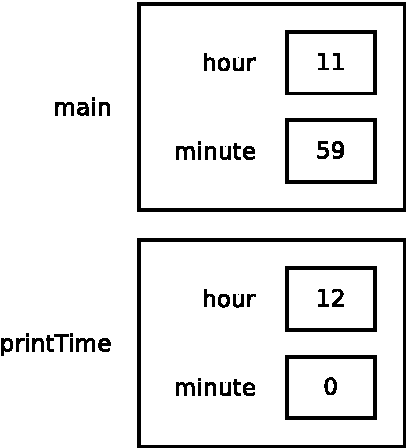
\includegraphics[height=15em]{figs/stack1.pdf}
\caption{Stack diagram for \java{printTime(hour + 1, 0)}.}
\label{fig.stack}
\end{center}
\end{figure}

As with memory diagrams, stack diagrams show variables and methods at a particular point in time.
Figure~\ref{fig.stack} is a stack diagram at the beginning of the \java{printTime} method.
Notice that \java{main} is on top, because it executed first.

%\index{scope}

%Stack diagrams help you to visualize the {\bf scope} of a variable, which is the area of a program where a variable exists.

\index{Java Tutor}
\index{tracing}

Stack diagrams are a good mental model for how variables and methods work at run-time.
Learning to trace the execution of a program on paper (or on a whiteboard) is a useful skill for communicating with other programmers.

There are educational tools that automatically draw stack diagrams for you.
For example, Java Tutor (\url{http://pythontutor.com/java.html}) allows you to step through an entire program, both forwards and backwards, and see the stack frames and variables at each step.
If you haven't already, you should check out the Java examples on that website.

%Or you can use a ``debugger'', like the one that comes with DrJava (see Appendix~\ref{debugger}).
%These tools also allow you to visualize the flow of execution.


\section{Return values}

\index{void}

When you invoke a \java{void} method, the invocation is usually on a line all by itself.
For example:

\begin{code}
printTime(hour + 1, 0);
\end{code}

On the other hand, when you invoke a value-returning method, you have to do something with the return value.
We usually assign it to a variable or use it as part of an expression, like this:

\begin{code}
double error = Math.abs(expect - actual);
double height = radius * Math.sin(angle);
\end{code}

\index{value method}
\index{method!value}

Compared to \java{void} methods, value-returning methods differ in two ways:

\index{return type}
\index{return value}

\begin{itemize}

\item They declare the type of the return value (the {\bf return type});

\item They use at least one \java{return} statement to provide a {\bf return value}.

\end{itemize}

Here's an example from a program named {\tt Circle.java}.
The \java{calculateArea} method takes a \java{double} as a parameter and returns the area of a circle with that radius (i.e., $\pi r^2$).

\begin{code}
public static double calculateArea(double radius) {
    double result = Math.PI * radius * radius;
    return result;
}
\end{code}

As usual, this method is \java{public} and \java{static}.
But in the place where we are used to seeing \java{void}, we see \java{double}, which means that the return value from this method is a \java{double}.

\index{return}
\index{statement!return}

The last line is a new form of the \java{return} statement that means, ``return immediately from this method, and use the following expression as the return value.''
The expression you provide can be arbitrarily complex, so we could have written this method more concisely:

\begin{code}
public static double calculateArea(double radius) {
    return Math.PI * radius * radius;
}
\end{code}

\index{temporary variable}
\index{variable!temporary}

On the other hand, {\bf temporary variables} like \java{result} often make debugging easier, especially when you are stepping through code using an interactive debugger (see Appendix~\ref{debugger}).

Figure~\ref{fig.param} illustrates how data values flows through the program.
When the \java{main} method invokes \java{calculateArea}, the value \java{5.0} is assigned to the parameter \java{radius}.
\java{calculateArea} then returns the value \java{78.54}, which is assigned to the variable \java{area}.
%Note that you don't ``pass variables'' as arguments and return values -- you copy their values.

\begin{figure}[!ht]
\begin{center}
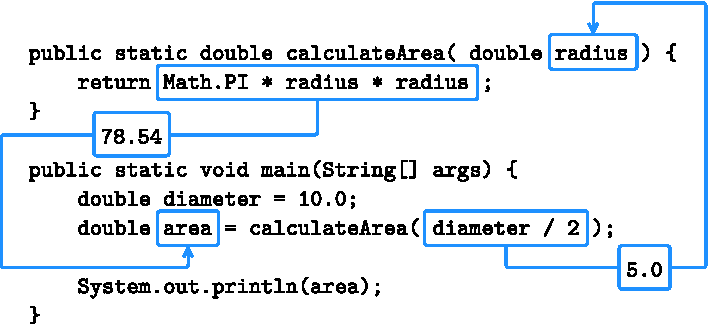
\includegraphics{figs/param.pdf}
\caption{Passing a parameter and saving the return value.}
\label{fig.param}
\end{center}
\end{figure}

The type of the expression in the \java{return} statement must match the return type of the method itself.
When you declare that the return type is \java{double}, you are making a promise that this method will eventually produce a \java{double} value.
If you try to \java{return} with no expression, or \java{return} an expression with the wrong type, the compiler will give an error.


\section{Incremental development}
\label{distance}

\index{incremental development}
\index{design process}

People often make the mistake of writing a lot of code before they try to compile and run it.
Then they spend way too much time debugging.
A better approach is what we call {\bf incremental development}.
The key aspects of incremental development are:

\begin{itemize}

\item Start with a working program and make small, incremental changes.
At any point, if there is an error, you will know where to look.

\item Use variables to hold intermediate values so you can check them, either with print statements or by using a debugger.

\item Once the program is working, you can consolidate multiple statements into compound expressions (but only if it does not make the program more difficult to read).

\end{itemize}

As an example, suppose you want to find the distance between two points, given by the coordinates $(x_1, y_1)$ and $(x_2, y_2)$.
By the usual definition:

\[ distance = \sqrt{(x_2 - x_1)^2 +(y_2 - y_1)^2} \]

The first step is to consider what a \java{distance} method should look like in Java.
In other words, what are the inputs (parameters) and what is the output (return value)?
For this method, the parameters are the two points, and it is natural to represent them using four \java{double} values.
%, although we will see later that there is a \java{Point} object in Java that we could use.
The return value is the distance, which should also have type \java{double}.

\index{stub}

Already we can write an outline for the method, which is sometimes called a {\bf stub}.
The stub includes the method declaration and a \java{return} statement:

\begin{code}
public static double distance
        (double x1, double y1, double x2, double y2) {
    return 0.0;  // stub
}
\end{code}

The return statement is a placeholder that is only necessary for the program to compile.
At this stage the program doesn't do anything useful, but it is good to compile it so we can find any syntax errors before we add more code.

\index{testing}

It's usually a good idea to think about testing {\em before} you develop new methods; doing so can help you figure out how to implement them.
To test the method, we can invoke it from \java{main} using the sample values:

\begin{code}
double dist = distance(1.0, 2.0, 4.0, 6.0);
\end{code}

With these values, the horizontal distance is 3.0 and the vertical distance is 4.0.
So the result should be 5.0, the hypotenuse of a 3-4-5 triangle.
When you are testing a method, it is necessary to know the right answer.

Once we have compiled the stub, we can start adding code one line at a time.
After each incremental change, we recompile and run the program.
If there is an error, we have a good idea where to look: the lines we just added.

The next step is to find the differences $x_2 - x_1$ and $y_2 - y_1$.
We store those values in temporary variables named \java{dx} and \java{dy}, so that we can examine them with print statements before proceeding.
They should be 3.0 and 4.0.

\begin{code}
public static double distance
        (double x1, double y1, double x2, double y2) {
    double dx = x2 - x1;
    double dy = y2 - y1;
    System.out.println("dx is " + dx);
    System.out.println("dy is " + dy);
    return 0.0;  // stub
}
\end{code}

\index{scaffolding}

We will remove the print statements when the method is finished.
Code like that is called {\bf scaffolding}, because it is helpful for building the program, but it is not part of the final product.

The next step is to square \java{dx} and \java{dy}.
We could use the \java{Math.pow} method, but it is simpler (and more efficient) to multiply each term by itself.

\begin{code}
public static double distance
        (double x1, double y1, double x2, double y2) {
    double dx = x2 - x1;
    double dy = y2 - y1;
    double dsquared = dx * dx + dy * dy;
    System.out.println("dsquared is " + dsquared);
    return 0.0;  // stub
}
\end{code}

Again, you should compile and run the program at this stage and check the intermediate value, which should be 25.0.
Finally, we can use \java{Math.sqrt} to compute and return the result.

\begin{code}
public static double distance
        (double x1, double y1, double x2, double y2) {
    double dx = x2 - x1;
    double dy = y2 - y1;
    double dsquared = dx * dx + dy * dy;
    double result = Math.sqrt(dsquared);
    return result;
}
\end{code}

%In \java{main}, we can print and check the value of the result.

As you gain more experience programming, you might write and debug more than one line at a time.
%Nevertheless, incremental development can save you a lot of time debugging.
But by using incremental development, scaffolding, and testing, your code is more likely to be correct the first time.


\section{Method composition}

\index{composition}

Once you define a method, you can use it to build other methods.
For example, suppose someone gave you two points -- the center of a circle and a point on the perimeter -- and asked for the area of the circle.

Let's say the center point is stored in the variables \java{xc} and \java{yc}, and the perimeter point is in \java{xp} and \java{yp}.
The first step is to find the radius of the circle, which is the distance between the two points.
Fortunately, we have a method that does just that.

\begin{code}
double radius = distance(xc, yc, xp, yp);
\end{code}

The second step is to find the area of a circle with that radius.
We have a method for that computation too.

\begin{code}
double area = calculateArea(radius);
\end{code}

Putting everything together in a new method, we get:

\begin{code}
public static double circleArea
        (double xc, double yc, double xp, double yp) {
    double radius = distance(xc, yc, xp, yp);
    double area = calculateArea(radius);
    return area;
}
\end{code}

Temporary variables like \java{radius} and \java{area} are useful for development and debugging, but once the program is working we can make it more concise by composing the method calls:

\begin{code}
public static double circleArea
        (double xc, double yc, double xp, double yp) {
    return calculateArea(distance(xc, yc, xp, yp));
}
\end{code}

\index{functional decomposition}

This example demonstrates a process known as {\bf functional decomposition}.
We broke a complex computation into simple methods, tested the methods in isolation, and then composed the methods to perform the final computation.
%This process reduces debugging time and yields code that is more likely to be correct and easier to maintain.

%Computer scientists deal with the complexity of large programs by breaking down computations into simpler methods (which in turn may call other methods).
%Data is passed around the program via parameters and return values.


\section{Overloading methods}

You might have noticed that \java{circleArea} and \java{calculateArea} perform similar functions.
They both find the area of a circle, but they take different parameters.
For \java{calculateArea}, we have to provide the radius; for \java{circleArea} we provide two points.

\index{overload}

If two methods do the same thing, it is natural to give them the same name.
Having more than one method with the same name is called {\bf overloading}, and it is legal in Java as long as each version of the method takes different parameters.
So we could rename \java{circleArea} to \java{calculateArea}:

\begin{code}
public static double calculateArea
        (double xc, double yc, double xp, double yp) {
    return calculateArea(distance(xc, yc, xp, yp));
}
\end{code}

%Note that this new \java{calculateArea} method is {\em not} recursive.
When you invoke an overloaded method, Java knows which version you want by looking at the arguments that you provide.

\begin{itemize}

\item For \java{calculateArea(3.0)}, Java uses the original \java{calculateArea} method that takes a \java{double} as an argument and interprets it as the radius.

\item For \java{calculateArea(1.0, 2.0, 4.0, 6.0)}, Java uses the new version of \java{calculateArea} (renamed from \java{circleArea}), which interprets the arguments as two points.

\end{itemize}

In fact, the second version of \java{calculateArea} invokes the first version (after invoking the \java{distance} method).

Many Java library methods are overloaded, meaning that there are different versions that accept different numbers or types of parameters.
For example, there are variants of \java{print} and \java{println} that accept a single parameter of any data type.
In the \java{Math} class, there is a version of \java{abs} that works on \java{double}s, and there is also a version for \java{int}s.

Although overloading is a useful feature, it should be used with caution.
You might get yourself nicely confused if you are trying to debug one version of a method while accidentally invoking a different one.


\section{Vocabulary}

\begin{description}

% Note: expanded definition from Chapter 1
%\term{method}
%A named sequence of statements that performs a procedure or function.
%Methods may or may not take parameters, and may or may not return a value.

%\term{void}
%A special return type indicating the method does not return a value.

\term{invoke}
To cause a method to execute.
Also known as ``calling'' a method.

\term{flow of execution}
The order in which Java executes methods and statements.
It may not necessarily be from top to bottom in the source file.

\term{parameter}
A piece of information that a method requires before it can run.
Parameters are variables: they contain values and have types.

\term{parameter passing}
The process of assigning an argument value to a parameter variable.

\term{local variable}
A variable declared inside a method.
Local variables cannot be accessed from outside their method.

\term{stack diagram}
A graphical representation of the variables belonging to each method.
The method calls are ``stacked'' from top to bottom, in the flow of execution.

\term{frame}
In a stack diagram, a representation of the variables and parameters for a method, along with their current values.

%\term{scope}
%The area of a program where a variable exists.

\term{return type}
The type of value a method returns.

\term{return value}
The value provided as the result of a method invocation.

\term{temporary variable}
A short-lived variable, often used for debugging.

\term{incremental development}
A process for creating programs by writing a few lines at a time, compiling, and testing.

\term{stub}
A placeholder for an incomplete method so that the class will compile.

\term{scaffolding}
Code that is used during program development but is not part of the final version.

\term{functional decomposition}
A process for breaking down a complex computation into simple methods, then composing the methods to perform the computation.

\term{overload}
To define more than one method with the same name but with different parameters.
%When you invoke an overloaded method, Java knows which version to use by looking at the arguments you provide.

\end{description}


\section{Exercises}

The code for this chapter is in the {\tt ch05} directory of {\tt ThinkJavaCode2}.
See page~\pageref{code} for instructions on how to download the repository.
Before you start the exercises, we recommend that you compile and run the examples.

If you have not already read Appendix~\ref{checkstyle}, now might be a good time.
It describes Checkstyle, a tool that analyzes many aspects of your source code.


\begin{exercise}  %%V6 Ex4.3

The purpose of this exercise is to take code from a previous exercise and redesign it as a method that takes parameters.
You should start with a working solution to Exercise~\ref{ex:date}.

\begin{enumerate}

\item Write a method called \java{printAmerican} that takes the day, date, month and year as parameters and that displays them in American format.

\item Test your method by invoking it from \java{main} and passing appropriate arguments.
The output should look something like this (except that the date might be different):

\begin{stdout}
Saturday, July 22, 2015
\end{stdout}

\item Once you have debugged \java{printAmerican}, write another method called \java{printEuropean} that displays the date in European format.

\end{enumerate}

\end{exercise}


\begin{exercise}  %%V6 Ex5.6

This exercise reviews the flow of execution through a program with multiple methods.
Read the following code and answer the questions.

\begin{code}
public static void baffle(String blimp) {
    System.out.println(blimp);
    zippo("ping", -5);
}
\end{code}

\begin{code}
public static void zippo(String quince, int flag) {
    if (flag < 0) {
        System.out.println(quince + " zoop");
    } else {
        System.out.println("ik");
        baffle(quince);
        System.out.println("boo-wa-ha-ha");
    }
}
\end{code}

\begin{code}
public static void main(String[] args) {
    zippo("rattle", 13);
}
\end{code}

\begin{enumerate}

\item Write the number {\tt 1} next to the first line of code in this program that will execute.

\item Write the number {\tt 2} next to the second line of code, and so on until the end of the program.
If a line is executed more than once, it might end up with more than one number next to it.

\item What is the value of the parameter \java{blimp} when \java{baffle} gets invoked?

\item What is the output of this program?

\end{enumerate}

\end{exercise}


\begin{exercise}  %%V6 Ex4.1

%The point of this exercise is to practice reading code and to make sure that you understand the flow of execution through a program with multiple methods.
Answer the following questions without running the program on a computer.

\begin{enumerate}

\item Draw a stack diagram that shows the state of the program the first time \java{ping} is invoked.

\item What is output by the following program?
Be precise about where there are spaces and where there are newlines.

%{\it Hint:} Start by describing in words what \java{ping} and \java{baffle} output.

%\item What happens if you invoke \java{baffle();} at the end of the \java{ping} method? (We will see why in Section~\ref{recursion}.)

\end{enumerate}

\begin{code}
public static void zoop() {
    baffle();
    System.out.print("You wugga ");
    baffle();
}
\end{code}

\begin{code}
public static void main(String[] args) {
    System.out.print("No, I ");
    zoop();
    System.out.print("I ");
    baffle();
}
\end{code}

\begin{code}
public static void baffle() {
    System.out.print("wug");
    ping();
}
\end{code}

\begin{code}
public static void ping() {
    System.out.println(".");
}
\end{code}

\end{exercise}


\begin{exercise}  %%V6 Ex6.1

If you have a question about whether something is legal, and what happens if it is not, a good way to find out is to ask the compiler.
Answer the following questions by trying them out.

\begin{enumerate}

\item What happens if you invoke a value method and don't do anything with the result; that is, if you don't assign it to a variable or use it as part of a larger expression?

\item What happens if you use a void method as part of an expression?
For example, try \java{System.out.println("boo!") + 7;}

\end{enumerate}

\end{exercise}


\begin{exercise}  %%V6 Ex5.2

Draw a stack diagram that shows the state of the program the {\it second} time \java{zoop} is invoked.
What is the complete output?

\begin{code}
public static void zoop(String fred, int bob) {
    System.out.println(fred);
    if (bob == 5) {
        ping("not ");
    } else {
        System.out.println("!");
    }
}
\end{code}

\begin{code}
public static void main(String[] args) {
    int bizz = 5;
    int buzz = 2;
    zoop("just for", bizz);
    clink(2 * buzz);
}
\end{code}

\begin{code}
public static void clink(int fork) {
    System.out.print("It's ");
    zoop("breakfast ", fork);
}
\end{code}

\begin{code}
public static void ping(String strangStrung) {
    System.out.println("any " + strangStrung + "more ");
}
\end{code}

\end{exercise}


\newpage
\begin{exercise}  %%V6 Ex6.5

What is the output of the following program?
Determine the answer without using a computer.

\begin{code}
public static void main(String[] args) {
    boolean flag1 = isHoopy(202);
    boolean flag2 = isFrabjuous(202);
    System.out.println(flag1);
    System.out.println(flag2);
    if (flag1 && flag2) {
        System.out.println("ping!");
    }
    if (flag1 || flag2) {
        System.out.println("pong!");
    }
}
\end{code}

\begin{code}
public static boolean isHoopy(int x) {
    boolean hoopyFlag;
    if (x % 2 == 0) {
        hoopyFlag = true;
    } else {
        hoopyFlag = false;
    }
    return hoopyFlag;
}
\end{code}

\begin{code}
public static boolean isFrabjuous(int x) {
    boolean frabjuousFlag;
    if (x > 0) {
        frabjuousFlag = true;
    } else {
        frabjuousFlag = false;
    }
    return frabjuousFlag;
}
\end{code}

The purpose of this exercise is to make sure you understand logical operators and the flow of execution through value methods.

\end{exercise}


\begin{exercise}  %%V6 Ex6.4

Many computations can be expressed more concisely using the ``multadd'' operation, which takes three operands and computes \java{a * b + c}.
Some processors even provide a hardware implementation of this operation for floating-point numbers.

\begin{enumerate}

\item Create a new program called {\tt Multadd.java}.

\item Write a method called \java{multadd} that takes three \java{doubles} as parameters and that returns \java{a * b + c}.

\item Write a \java{main} method that tests \java{multadd} by invoking it with a few simple parameters, like \java{1.0, 2.0, 3.0}.

\item Also in \java{main}, use \java{multadd} to compute the following values:
%
\begin{eqnarray*}
& \sin \frac{\pi}{4} + \frac{\cos \frac{\pi}{4}}{2} & \\
& \log 10 + \log 20 &
\end{eqnarray*}

\item Write a method called \java{expSum} that takes a double as a parameter and that uses \java{multadd} to calculate:
%
\begin{eqnarray*}
x e^{-x} + \sqrt{1 - e^{-x}}
\end{eqnarray*}
%
{\it Hint:} The method for raising $e$ to a power is \java{Math.exp}.

\end{enumerate}

In the last part of this exercise, you need to write a method that invokes another method you wrote.
Whenever you do that, it is a good idea to test the first method carefully before working on the second.
Otherwise, you might find yourself debugging two methods at the same time, which can be difficult.

One of the purposes of this exercise is to practice pattern-matching: the ability to recognize a specific problem as an instance of a general category of problems.

\end{exercise}


\chapter{Loops and strings}

Computers are often used to automate repetitive tasks, such as searching for text in documents.
Repeating tasks without making errors is something that computers do well and people do poorly.

In this chapter, we'll learn how to use \java{while} and \java{for} loops to add repetition to your code.
We'll also take a first look at \java{String} methods and solve some interesting problems.

%We have seen methods, like \java{countdown} and \java{factorial}, that use recursion to iterate.
%Although recursion is elegant and powerful, it takes some getting used to.
%Java provides language features that make iteration much easier: the \java{while} and \java{for} statements.


\section{The while statement}

\index{while}
\index{loop!while}
\index{statement!while}

Using a \java{while} statement, we can repeat the same code multiple times:

\begin{code}
int n = 3;
while (n > 0) {
    System.out.println(n);
    n = n - 1;
}
System.out.println("Blastoff!");
\end{code}

Reading the code in English sounds like: ``Start with \java{n} set to 3.
While \java{n} is greater than zero, print the value of \java{n}, and reduce the value of \java{n} by 1.
When you get to zero, print Blastoff!''
So the output is:

\begin{stdout}
3
2
1
Blastoff!
\end{stdout}

The flow of execution for a \java{while} statement is:

\begin{enumerate}

\item Evaluate the condition in parentheses, yielding \java{true} or \java{false}.

\item If the condition is \java{false}, skip the following statements in braces.

\item If the condition is \java{true}, execute the statements and go back to step 1.

\end{enumerate}

\index{loop}

This type of flow is called a {\bf loop}, because the last step ``loops back around'' to the first.
Figure~\ref{fig.while} shows this idea using a flowchart.

\begin{figure}[!ht]
\begin{center}
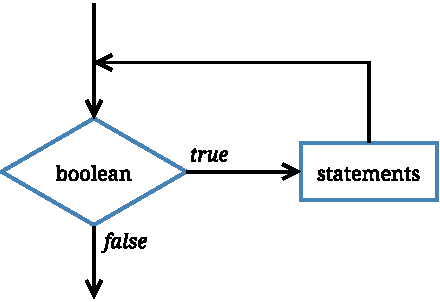
\includegraphics[scale=0.9]{figs/while.pdf}
\caption{Flow of execution for a \java{while} loop.}
\label{fig.while}
\end{center}
\end{figure}

\index{loop body}
\index{infinite loop}
\index{loop!infinite}

The {\bf body} of the loop should change the value of one or more variables so that, eventually, the condition becomes \java{false} and the loop terminates.
Otherwise the loop will repeat forever, which is called an {\bf infinite loop}.

\begin{code}
int n = 3;
while (n > 0) {
    System.out.println(n);
    // n never changes
}
\end{code}

This example will print the number \java{3} forever, or at least until you terminate the program.
An endless source of amusement for computer scientists is the observation that the directions on shampoo, ``Lather, rinse, repeat,'' are an infinite loop.

In the first example, we can prove that the loop terminates when \java{n} is positive.
But in general, it is not so easy to tell whether a loop terminates.
For example, this loop continues until \java{n} is 1 (which makes the condition \java{false}):

\begin{code}
while (n != 1) {
    System.out.println(n);
    if (n % 2 == 0) {         // n is even
        n = n / 2;
    } else {                  // n is odd
        n = 3 * n + 1;
    }
}
\end{code}

Each time through the loop, the program displays the value of \java{n} and then checks whether it is even or odd.
If it is even, the value of \java{n} is divided by two.
If it is odd, the value is replaced by $3n+1$.
For example, if the starting value is 3, the resulting sequence is 3, 10, 5, 16, 8, 4, 2, 1.

Since \java{n} sometimes increases and sometimes decreases, there is no obvious proof that \java{n} will ever reach 1 and that the program will ever terminate.
For some values of \java{n}, such as the powers of two, we can prove that it terminates.
The previous example ends with such a sequence, starting when \java{n} is 16 (or $2^4$).

The hard question is whether this program terminates for {\em all} values of n.
So far, no one has been able to prove it {\em or} disprove it!
For more information, see \url{https://en.wikipedia.org/wiki/Collatz_conjecture}.
%The field of computer science is interested in these types of questions, because their answers give insight to the limits of what computers can and cannot do.


\section{Increment and decrement}

Here is another \java{while} loop example; this one displays the numbers 1 to 5.

\begin{code}
int i = 1;
while (i <= 5) {
    System.out.println(i);
    i++;  // add 1 to i
}
\end{code}

\index{increment}
\index{decrement}

Assignments like \java{i = i + 1} don't often appear in loops, because Java provides a more concise way to add and subtract by one.
Specifically, \java{++} is the {\bf increment} operator; it has the same effect as \java{i = i + 1}.
And \java{--} is the {\bf decrement} operator; it has the same effect as \java{i = i - 1}.

%So far in this book we have only used (\java{=}) to assign values to variables.
%For convenience, Java provides other assignment operators that increase or decrease the value of a variable.

If you want to increment or decrement a variable by an amount other than \java{1}, you can use \java{+=} and \java{-=}.
For example, \java{i += 2} increments \java{i} by \java{2}.

\begin{code}
int i = 2;
while (i <= 8) {
    System.out.print(i + ", ");
    i += 2;  // add 2 to i
}
System.out.println("Who do we appreciate?");
\end{code}

And the output is:

\begin{stdout}
2, 4, 6, 8, Who do we appreciate?
\end{stdout}


\section{The for statement}

\index{for}
\index{loop!for}
\index{statement!for}

The loops we have written so far have several elements in common.
They start by initializing a variable, they have a condition that depends on that variable, and inside the loop they do something to update that variable.

\index{iteration}

Running the same code multiple times is called {\bf iteration}.
This type of loop is so common that there is another statement, the \java{for} loop, that expresses it more concisely.
For example, we can rewrite the 2-4-6-8 loop this way:

\begin{code}
for (int i = 2; i <= 8; i += 2) {
    System.out.print(i + ", ");
}
System.out.println("Who do we appreciate?");
\end{code}

\java{for} loops have three components in parentheses, separated by semicolons: the initializer, the condition, and the update.

\begin{enumerate}

\item The {\em initializer} runs once at the very beginning of the loop.
(It is equivalent to the line before the \java{while} statement.)

\item The {\em condition} is checked each time through the loop.
If it is \java{false}, the loop ends.
Otherwise, the body of the loop is executed (again).

\item At the end of each iteration, the {\em update} runs, and we go back to step~2.

\end{enumerate}

The \java{for} loop is often easier to read because it puts all the loop-related statements at the top of the loop.
Doing so allows you to focus on the statements in the loop body.
Figure~\ref{fig.for} illustrates \java{for} loops with a flowchart.

\begin{figure}[!ht]
\begin{center}
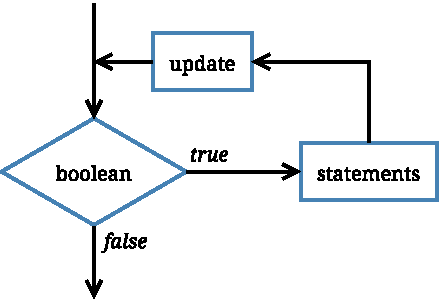
\includegraphics[scale=0.9]{figs/for.pdf}
\caption{Flow of execution for a \java{for} loop.}
\label{fig.for}
\end{center}
\end{figure}

There is another difference between \java{for} loops and \java{while} loops: if you declare a variable in the initializer, it only exists {\em inside} the \java{for} loop.
For example:

\begin{code}
for (int n = 3; n > 0; n--) {
    System.out.println(n);
}
System.out.println("n is now " + n);  // compiler error
\end{code}

The last line tries to display \java{n} (for no reason other than demonstration) but it won't work.
If you need to use a loop variable outside the loop, you have to declare it {\em outside} the loop, like this:

\begin{code}
int n;
for (n = 3; n > 0; n--) {
    System.out.println(n);
}
System.out.println("n is now " + n);
\end{code}

Notice that the \java{for} statement does not say \java{int n = 3}.
Rather, it simply initializes the existing variable \java{n}.


\section{Nested loops}
\label{nested}

\index{loop!nested}
\index{nested!loops}

Like conditional statements, loops can be nested one inside the other.
Nested loops allow you to iterate over two variables.
For example, we can generate a ``multiplication table'' like this:

\begin{code}
for (int x = 1; x <= 10; x++) {
    for (int y = 1; y <= 10; y++) {
        System.out.printf("%4d", x * y);
    }
    System.out.println();
}
\end{code}

\index{loop variable}
\index{variable!loop}
\index{inner loop}
\index{outer loop}

Variables like \java{x} and \java{y} are called {\bf loop variables}, because they control the execution of a loop.
In this example, the first loop (\java{for x}) is known as the ``outer loop'', and the second loop (\java{for y}) is known as the ``inner loop''.

Each loop repeats their corresponding statements 10 times.
The outer loop iterates from 1 to 10 only once, but the inner loop iterates from 1 to 10 each of those 10 times.
As a result, the \java{printf} method is invoked 100 times.

\index{format specifier}

The format specifier \java{\%4d} displays the value of \java{x * y} padded with spaces so it's four characters wide.
Doing so causes the output to align vertically, regardless of how many digits the numbers have:

\begin{stdout}
   1   2   3   4   5   6   7   8   9  10
   2   4   6   8  10  12  14  16  18  20
   3   6   9  12  15  18  21  24  27  30
   4   8  12  16  20  24  28  32  36  40
   5  10  15  20  25  30  35  40  45  50
   6  12  18  24  30  36  42  48  54  60
   7  14  21  28  35  42  49  56  63  70
   8  16  24  32  40  48  56  64  72  80
   9  18  27  36  45  54  63  72  81  90
  10  20  30  40  50  60  70  80  90 100
\end{stdout}

It's important to realize that the output is displayed row by row.
The inner loop displays a single row of output, followed by a newline.
The outer loop iterates over the rows themselves.
Another way to read nested loops, like the ones in this example, is ``for each row \java{x}, and for each column \java{y}, \ldots''


\section{Characters}

Some of the most interesting problems in computer science involve searching and manipulating text.
In the next few sections, we'll discuss how to apply loops to strings.
Although the examples are short, the techniques work the same whether you have one word or one million words.

\index{charAt}
\index{char}
\index{type!char}

Strings provide a method named \java{charAt}.
It returns a \java{char}, a data type that stores an individual character (as opposed to strings of them).

\begin{code}
String fruit = "banana";
char letter = fruit.charAt(0);
\end{code}

The argument \java{0} means that we want the character at {\bf index} 0.
String indexes range from 0 to $n-1$, where $n$ is the length of the string.
So the character assigned to \java{letter} is \java{b}.

\begin{center}
\ttfamily
\begin{tabular}{cccccc}
\hline
\multicolumn{1}{|l|}{b} & \multicolumn{1}{l|}{a} & \multicolumn{1}{l|}{n} & \multicolumn{1}{l|}{a} & \multicolumn{1}{l|}{n} & \multicolumn{1}{l|}{a} \\ \hline
0                       & 1                      & 2                      & 3                      & 4                      & 5
\end{tabular}
\end{center}


Characters work like the other data types we have seen.
You can compare them using relational operators:

\begin{code}
if (letter == 'a') {
    System.out.println('?');
}
\end{code}

\index{quote mark}
\index{escape sequence}

Character literals, like \java{'a'}, appear in single quotes.
Unlike string literals, which appear in double quotes, character literals can only contain a single character.
Escape sequences, like \java{'\\t'}, are legal because they represent a single character.

The increment and decrement operators also work with characters.
So this loop displays the letters of the alphabet:

\begin{code}
System.out.print("Roman alphabet: ");
for (char c = 'A'; c <= 'Z'; c++) {
    System.out.print(c);
}
System.out.println();
\end{code}

\index{Unicode}

Java uses {\bf Unicode} to represent characters, so strings can store text in other alphabets like Cyrillic and Greek, and non-alphabetic languages like Chinese.
You can read more about it at \url{http://unicode.org/}.

In Unicode, each character is represented by a ``code point'', which you can think of as an integer.
The code points for uppercase Greek letters run from 913 to 937, so we can display the Greek alphabet like this:

\begin{code}
System.out.print("Greek alphabet: ");
for (int i = 913; i <= 937; i++) {
    System.out.print((char) i);
}
System.out.println();
\end{code}

This example uses a type cast to convert each integer (in the range) to the corresponding character.
Try running the code and see what happens.


\section{String iteration}

\index{iteration}

The following loop iterates the characters in \java{fruit} and displays them, one on each line:

\begin{code}
for (int i = 0; i < fruit.length(); i++) {
    char letter = fruit.charAt(i);
    System.out.println(letter);
}
\end{code}

\index{string!length}
\index{length!string}

Strings provide a method called \java{length} that returns the number of characters in the string.
Because it is a method, you have to invoke it with the empty argument list, \java{()}.
When \java{i} is equal to the length of the string, the condition becomes \java{false} and the loop terminates.

To find the last letter of a string, you might be tempted to do something like:

\begin{code}
int length = fruit.length();
char last = fruit.charAt(length);      // wrong!
\end{code}

\index{StringIndexOutOfBoundsException}
\index{exception!StringIndexOutOfBounds}

This code compiles and runs, but invoking the \java{charAt} method throws a \java{StringIndexOutOfBoundsException}.
The problem is that there is no sixth letter in \java{"banana"}.
Since we started counting at 0, the 6 letters are indexed from 0 to 5.
To get the last character, you have to subtract 1 from \java{length}.

\begin{code}
int length = fruit.length();
char last = fruit.charAt(length - 1);  // correct
\end{code}

Many string algorithms involve reading one string and building another.
For example, to reverse a string, we can add one character at a time:

\begin{code}
public static String reverse(String s) {
    String r = "";
    for (int i = s.length() - 1; i >= 0; i--) {
        r += s.charAt(i);
    }
    return r;
}
\end{code}

\index{empty string}

The initial value of \java{r} is \java{""}, which is the {\bf empty string}.
The loop iterates the letters of \java{s} in reverse order.
Each time through the loop, it creates a new string and assigns it to \java{r}.
When the loop exits, \java{r} contains the letters from \java{s} in reverse order.
So the result of \java{reverse("banana")} is \java{"ananab"}.


\section{The indexOf method}

\index{indexOf}

To search for a specific character in a string, you could write a \java{for} loop and use \java{charAt} like in the previous section.
However, the \java{String} class already provides a method for doing just that.

\begin{code}
String fruit = "banana";
int index = fruit.indexOf('a');     // returns 1
\end{code}

This example finds the index of \java{'a'} in the string.
But the letter appears three times, so it's not obvious what \java{indexOf} should do.
According to the documentation, it returns the index of the {\em first} appearance.

To find subsequent appearances, you can use another version of \java{indexOf}, which takes a second argument that indicates where in the string to start looking.

\begin{code}
int index = fruit.indexOf('a', 2);  // returns 3
\end{code}

To visualize how \java{indexOf} and other \java{String} methods work, it helps to draw a picture like Figure~\ref{fig.banana}.
The previous code starts at index 2 (the first \java{'n'}) and finds the next \java{'a'}, which is at index 3.

\index{memory diagram}
\index{diagram!memory}

\begin{figure}[!ht]
\begin{center}
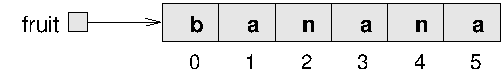
\includegraphics{figs/banana.pdf}
\caption{Memory diagram for a \java{String} of six characters.}
\label{fig.banana}
\end{center}
\end{figure}

%\begin{center}
%\begin{tabular}{c|c|c|c|c|c}
%%\hline
%b & a & n & a & n & a \\
%\hline
%0 & 1 & 2 & 3 & 4 & 5 \\
%%\hline
%\end{tabular}
%\end{center}

If the character happens to appear at the starting index, the starting index is the answer.
So \java{fruit.indexOf('a', 5)} returns \java{5}.
If the character does not appear in the string, \java{indexOf} returns \java{-1}.
Since indexes cannot be negative, this value indicates the character was not found.

You can also use \java{indexOf} to search for an entire string, not just a single character.
For example, the expression \java{fruit.indexOf("nan")} returns \java{2}.


\section{String comparison}
\label{strcmp}

\index{equals}
\index{string!comparing}

To compare two strings, it may be tempting to use the \java{==} and \java{!=} operators.

\begin{code}
String name1 = "Alan Turing";
String name2 = "Ada Lovelace";
if (name1 == name2) {                 // wrong!
    System.out.println("The names are the same.");
}
\end{code}

This code compiles and runs, and sometimes it gets the answer right.
But sometimes it gets the answer wrong.
If you give it two different strings that contain the same letters, the condition will be \java{false}.

The problem is that the \java{==} operator checks whether the two variables refer to the {\em same object} by comparing the references.
We'll learn more about references in the next chapter.
The correct way to compare strings is with the \java{equals} method, like this:

\begin{code}
if (name1.equals(name2)) {
    System.out.println("The names are the same.");
}
\end{code}

This example invokes \java{equals} on \java{name1} and passes \java{name2} as an argument.
The \java{equals} method returns \java{true} if the strings contain the same characters; otherwise it returns \java{false}.

\index{compareTo}

If the strings differ, we can use \java{compareTo} to see which comes first in alphabetical order:

\begin{code}
int diff = name1.compareTo(name2);
if (diff == 0) {
    System.out.println("The names are the same.");
} else if (diff < 0) {
    System.out.println("name1 comes before name2.");
} else if (diff > 0) {
    System.out.println("name2 comes before name1.");
}
\end{code}

The return value from \java{compareTo} is the difference between the first characters in the strings that are not the same.
In the preceding code, \java{compareTo} returns positive 8, because the second letter of \java{"Ada"} comes before the second letter of \java{"Alan"} by 8 letters.

If the strings are equal, their difference is zero.
If the first string (the one on which the method is invoked) comes first in the alphabet, the difference is negative.
Otherwise, the difference is positive.

\index{case-sensitive}

Both \java{equals} and \java{compareTo} are case-sensitive.
In Unicode, uppercase letters come before lowercase letters.
So \java{"Ada"} comes before \java{"ada"}.


\section{Substrings}

\index{substring}

The \java{substring} method returns a new string that copies letters from an existing string, starting at the given index.

\begin{itemize}
\item \java{fruit.substring(0)} returns \java{"banana"}
\item \java{fruit.substring(2)} returns \java{"nana"}
\item \java{fruit.substring(6)} returns \java{""}
\end{itemize}

The first example returns a copy of the entire string.
The second example returns all but the first two characters.
As the last example shows, \java{substring} returns the empty string if the argument is the length of the string.

Like most string methods, \java{substring} is overloaded.
That is, there are other versions of \java{substring} that have different parameters.
If it's invoked with two arguments, they are treated as a start and end index:

\begin{itemize}
\item \java{fruit.substring(0, 3)} returns \java{"ban"}
\item \java{fruit.substring(2, 5)} returns \java{"nan"}
\item \java{fruit.substring(6, 6)} returns \java{""}
\end{itemize}

Notice that the character indicated by the end index is {\em not} included.
Defining \java{substring} this way simplifies some common operations.
For example, to select a substring with length \java{len}, starting at index \java{i}, you could write \java{fruit.substring(i, i + len)}.
%So \java{fruit.substring(2, 2 + 3)} returns \java{"nan"}.


\section{String formatting}

\index{printf}

In Section~\ref{printf}, we learned how to use \java{System.out.printf} to display formatted output.
Sometimes programs need to create strings that are formatted a certain way, but not display them immediately, or ever.
For example, the following method returns a time string in 12-hour format:

\begin{code}
public static String timeString(int hour, int minute) {
    String ampm;
    if (hour < 12) {
        ampm = "AM";
        if (hour == 0) {
            hour = 12;  // midnight
        }
    } else {
        ampm = "PM";
        hour = hour - 12;
    }
    return String.format("%02d:%02d %s", hour, minute, ampm);
}
\end{code}

\index{string!format}

\java{String.format} takes the same arguments as \java{System.out.printf}: a format specifier followed by a sequence of values.
The main difference is that \java{System.out.printf} displays the result on the screen.
\java{String.format} creates a new string, but does not display anything.

In this example, the format specifier \java{\%02d} means ``two digit integer padded with zeros'', so \java{timeString(19, 5)} returns the string \java{"07:05 PM"}.
As an exercise, try writing two nested \java{for} loops (in \java{main}) that invoke \java{timeString} and display all possible times over a 24-hour period.

At some point today, skim through the documentation for \java{String}.
Knowing what other methods are there will help you avoid reinventing the wheel.
The easiest way to find documentation for Java classes is to do a web search for ``Java'' and the name of the class.


\section{Vocabulary}

\begin{description}

\term{loop}
A statement that executes a sequence of statements repeatedly.

\term{loop body}
The statements inside the loop.

\term{infinite loop}
A loop whose condition is always true.

\term{increment}
Increase the value of a variable.

\term{decrement}
Decrease the value of a variable.

\term{iteration}
Executing a sequence of statements repeatedly.

\term{loop variable}
A variable that is initialized, tested, and updated in order to control a loop.

\term{index}
An integer variable or value used to indicate a character in a string.

\term{Unicode}
An international standard for representing characters in most of the world's languages.

\term{empty string}
The string \java{""}, which contains no characters and has a length of zero.

\end{description}


\section{Exercises}

The code for this chapter is in the {\tt ch06} directory of {\tt ThinkJavaCode2}.
See page~\pageref{code} for instructions on how to download the repository.
Before you start the exercises, we recommend that you compile and run the examples.

If you have not already read Appendix~\ref{debugger}, now might be a good time.
It describes the DrJava debugger, which is a useful tool for visualizing the flow of execution through loops.


\begin{exercise}  %%V6 Ex7.1

Consider the following methods:

\begin{code}
public static void main(String[] args) {
    loop(10);
}

public static void loop(int n) {
    int i = n;
    while (i > 1) {
        System.out.println(i);
        if (i % 2 == 0) {
            i = i / 2;
        } else {
            i = i + 1;
        }
    }
}
\end{code}

\begin{enumerate}

\item Draw a table that shows the value of the variables \java{i} and \java{n} during the execution of \java{loop}.
The table should contain one column for each variable and one line for each iteration.

\item What is the output of this program?

\item Can you prove that this loop terminates for any positive value of \java{n}?

% If i is odd and we increment by 1, the result is even.  So the second
% branch is always followed by the first branch.
% If i is even and we divide by 2, the result might be odd.  So in the
% worst case, we might alternate between the branches.
% But we can't do more of the second branch than the first.
% So we divide at least as often as we add.

% If i is 1, we're done.
% If i is 2, we divide by 2 and we're done.
% If i is greater than 2, the first branch decreases more than the
% second branch increases.
% So if we do one of each, the net effect is a decrease.
% Therefore, the value of i has to decrease after any two steps.

\end{enumerate}

\end{exercise}


\begin{exercise}  %%V6 Ex7.2

Let's say you are given a number, $a$, and you want to find its square root.
One way to do that is to start with a rough guess about the answer, $x_0$, and then improve the guess using this formula:
%
\[ x_1 =(x_0 + a/x_0) / 2 \]
%
For example, if we want to find the square root of 9, and we start with $x_0 = 6$, then $x_1 = (6 + 9/6) / 2 = 3.75$, which is closer.
We can repeat the procedure, using $x_1$ to calculate $x_2$, and so on.
In this case, $x_2 = 3.075$ and $x_3 = 3.00091$.
So it converges quickly on the correct answer.

Write a method called \java{squareRoot} that takes a \java{double} and returns an approximation of the square root of the parameter, using this technique.
You should not use \java{Math.sqrt}.

As your initial guess, you should use $a/2$.
Your method should iterate until it gets two consecutive estimates that differ by less than 0.0001.
%In other words, return when the absolute value of $x_n - x_{n-1}$ is less than 0.0001.
You can use \java{Math.abs} to calculate the absolute value of the difference.

\end{exercise}


\begin{exercise}  %%V6 Ex7.6

One way to evaluate $\exp(-x^2)$ is to use the infinite series expansion:
%
\[ \exp(-x^2) = 1 - x^2 + x^4/2 - x^6/6 + \ldots \]
%
The $i$th term in this series is $(-1)^i x^{2i} / i!$.
Write a method named \java{gauss} that takes \java{x} and \java{n} as arguments and returns the sum of the first \java{n} terms of the series.
You should not use \java{factorial} or \java{pow}.

\end{exercise}


\begin{exercise}  %%V6 Ex9.5

\index{abecedarian}

A word is said to be ``abecedarian'' if the letters in the word appear in alphabetical order.
For example, the following are all six-letter English abecedarian words:

\begin{quote}
abdest, acknow, acorsy, adempt, adipsy, agnosy, befist, behint, %\\
beknow, bijoux, biopsy, cestuy, chintz, deflux, dehors, dehort, %\\
deinos, diluvy, dimpsy %\\
\end{quote}

Write a method called \java{isAbecedarian} that takes a \java{String} and returns a \java{boolean} indicating whether the word is abecedarian.
%Your method can be iterative or recursive.

\end{exercise}


\begin{exercise}  %%V6 Ex9.6
\label{doubloon}

\index{doubloon}

A word is said to be a ``doubloon'' if every letter that appears in the word appears exactly twice.
Here are some example doubloons found in the dictionary:

\begin{quote}
Abba, Anna, appall, appearer, appeases, arraigning, beriberi, bilabial, boob, Caucasus, coco, Dada, deed, Emmett, Hannah, horseshoer, intestines, Isis, mama, Mimi, murmur, noon, Otto, papa, peep, reappear, redder, sees, Shanghaiings, Toto
\end{quote}

Write a method called \java{isDoubloon} that takes a string and checks whether it is a doubloon.
To ignore case, invoke the \java{toLowerCase} method before checking.
\end{exercise}


\begin{exercise}  %%V6 Ex9.8

\index{Scrabble}

In Scrabble\footnote{Scrabble is a registered trademark owned in the USA and Canada by Hasbro Inc., and in the rest of the world by J.\ W.\ Spear \& Sons Limited of Maidenhead, Berkshire, England, a subsidiary of Mattel Inc.} each player has a set of tiles with letters on them.
The object of the game is to use those letters to spell words.
The scoring system is complex, but longer words are usually worth more than shorter words.

Imagine you are given your set of tiles as a string, like \java{"quijibo"}, and you are given another string to test, like \java{"jib"}.

Write a method called \java{canSpell} that takes two strings and checks whether the set of tiles can spell the word.
You might have more than one tile with the same letter, but you can only use each tile once.

\end{exercise}


\chapter{Arrays and references}

Up to this point, the only variables we have used were for individual values such as numbers or strings.
In this chapter, we'll learn how to store multiple values of the same type using a single variable.
This language feature will enable you to write programs that manipulate larger amounts of data.

For example, Exercise~\ref{doubloon} asked you to check whether every letter in a string appears exactly twice.
One algorithm (which hopefully you already discovered) is to loop through the string 26 times, once for each lowercase letter:

\begin{code}
for (char c = 'a'; c <= 'z'; c++) {
    // count how many times the letter appears
    // if the count is not 0 or 2, return false
}
\end{code}

This ``nested loops'' approach is inefficient, especially when the string is long (e.g., one billion characters).
Another algorithm would initialize 26 variables to zero, loop through the string once, and use a giant \java{if} statement update the variable for each letter.
But who wants to declare 26 variables?

That's where arrays come in.
We can declare a single variable that stores 26 integers.
Rather than use an \java{if} statement to update each value, we can use arithmetic to update the $n$th value directly.
We will present this algorithm at the end of the chapter.


\section{Creating arrays}

\index{array}
\index{element}

An {\bf array} is a sequence of values; the values in the array are called {\bf elements}.
You can make an array of \java{int}s, \java{double}s, \java{String}s, or any other type, but all the values in an array must have the same type.

\index{type!array}
\index{[ ] square brackets}
\index{brackets!square}

To create an array, you have to declare a variable with an {\em array type} and then create the array itself.
Array types look like other Java types, except they are followed by square brackets (\java{[]}).
For example, the following lines declare that \java{counts} is an ``integer array'' and \java{values} is a ``double array'':

\begin{code}
int[] counts;
double[] values;
\end{code}

\index{new}
\index{operator!new}
\index{allocate}

To create the array itself, you have to use the \java{new} operator, which we first saw in Section~\ref{scanner}.
The \java{new} operator {\bf allocates} memory for the array and automatically initializes all of its elements to zero.

\begin{code}
counts = new int[4];
values = new double[size];
\end{code}

The first assignment makes \java{counts} refer to an array of four integers.
The second makes \java{values} refer to an array of \java{double}s, but the number of elements depends on the value of \java{size} (at the time the array is created).

Of course, you can also declare the variable and create the array with a single line of code:

\begin{code}
int[] counts = new int[4];
double[] values = new double[size];
\end{code}

\index{NegativeArraySizeException}
\index{exception!NegativeArraySize}

You can use any integer expression for the size of an array, as long as the value is nonnegative.
If you try to create an array with \java{-4} elements, for example, you will get a \java{NegativeArraySizeException}.
An array with zero elements is allowed, and there are special uses for such arrays that we'll see later on.


\section{Accessing elements}
\label{elements}

When you create an array with the \java{new} operator, the elements are initialized to zero.
Figure~\ref{fig.array} shows a memory diagram of the \java{counts} array so far.

\begin{figure}[!ht]
\begin{center}
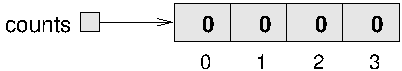
\includegraphics{figs/array.pdf}
\caption{Memory diagram of an \java{int} array.}
\label{fig.array}
\end{center}
\end{figure}

\index{reference}

The arrow indicates that the value of \java{counts} is a {\bf reference} to the array.
You should think of {\em the array} and {\em the variable} that refers to it as two different things.
As we'll soon see, we can assign a different variable to refer to the same array, and we can change the value of \java{counts} to refer to a different array.

\index{element}
\index{index}
\index{array!element}
\index{array!index}

The large numbers inside the boxes are the elements of the array.
The small numbers outside the boxes are the {\bf indexes} used to identify each location in the array.
As with strings, the index of the first element is 0, not 1.
For this reason, we sometimes refer to the first element as the ``zeroth'' element.

The \java{[]} operator selects elements from an array:

\begin{code}
System.out.println("The zeroth element is " + counts[0]);
\end{code}

You can use the \java{[]} operator anywhere in an expression:

\begin{code}
counts[0] = 7;
counts[1] = counts[0] * 2;
counts[2]++;
counts[3] -= 60;
\end{code}

Figure~\ref{fig.array2} shows the result of these statements.

\begin{figure}[!ht]
\begin{center}
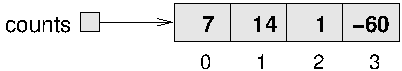
\includegraphics{figs/array2.pdf}
\caption{Memory diagram after several assignment statements.}
\label{fig.array2}
\end{center}
\end{figure}

You can use any expression as an index, as long as it has type \java{int}.
One of the most common ways to index an array is with a loop variable.
For example:

\begin{code}
int i = 0;
while (i < 4) {
    System.out.println(counts[i]);
    i++;
}
\end{code}

This \java{while} loop counts up from 0 to 4.
When \java{i} is 4, the condition fails and the loop terminates.
So the body of the loop is only executed when \java{i} is 0, 1, 2, and 3.
In this context, the variable name \java{i} is short for ``index''.

\index{loop variable}
\index{variable!loop}

Each time through the loop we use \java{i} as an index into the array, displaying the \java{i}th element.
This type of array processing is usually written as a \java{for} loop.

\begin{code}
for (int i = 0; i < 4; i++) {
    System.out.println(counts[i]);
}
\end{code}

\index{ArrayIndexOutOfBoundsException}
\index{exception!ArrayIndexOutOfBounds}

For the \java{counts} array, the only legal indexes are 0, 1, 2, and 3.
If the index is negative or greater than 3, the result is an \java{ArrayIndexOutOfBoundsException}.


\section{Displaying arrays}
\label{printarray}

\index{array!printing}

You can use \java{println} to display an array, but it probably doesn't do what you would like.
For example, the following fragment (1) declares an array variable, (2) makes it refer to an array of four elements, and (3) attempts to display the contents of the array using \java{println}:

\begin{code}
int[] a = {1, 2, 3, 4};
System.out.println(a);
\end{code}

Unfortunately, the output is something like:

\begin{stdout}
[I@bf3f7e0
\end{stdout}

The bracket indicates that the value is an array, \java{I} stands for ``integer'', and the rest represents the address of the array in memory.
If we want to display the elements of the array, we could do it ourselves:

\begin{code}
public static void printArray(int[] a) {
    System.out.print("{" + a[0]);
    for (int i = 1; i < a.length; i++) {
        System.out.print(", " + a[i]);
    }
    System.out.println("}");
}
\end{code}

Given the previous array, the output of \java{printArray} is:

\begin{stdout}
{1, 2, 3, 4}
\end{stdout}

\index{utility class}
\index{Arrays class}

The Java library provides a utility class \java{java.util.Arrays} that has methods for working with arrays.
One of them, \java{toString}, returns a string representation of an array.
We can invoke it like this:

\begin{code}
System.out.println(Arrays.toString(a));
\end{code}

And the output is:

\begin{stdout}
[1, 2, 3, 4]
\end{stdout}

As usual, we have to \java{import java.util.Arrays} before we can use it.
Notice that the string format is slightly different: it uses square brackets instead of curly braces.
But it beats having to write your own \java{printArray} method.


\section{Copying arrays}

\index{array!copying}

As explained in Section~\ref{elements}, array variables contain {\em references} to arrays.
When you make an assignment to an array variable, it simply copies the reference.
But it doesn't copy the array itself.
For example:

\begin{code}
double[] a = new double[3];
double[] b = a;
\end{code}

These statements create an array of three \java{double}s and make two different variables refer to it, as shown in Figure~\ref{fig.array3}.

\index{memory diagram}
\index{diagram!memory}

\begin{figure}[!ht]
\begin{center}
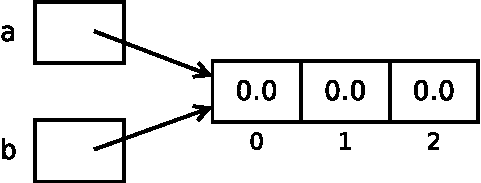
\includegraphics[scale=0.75]{figs/array3.pdf}
\caption{Memory diagram of two variables referring to the same array.}
\label{fig.array3}
\end{center}
\end{figure}

\index{alias}

Any changes made through either variable will be seen by the other.
For example, if we set \java{a[0] = 17.0}, and then display \java{b[0]}, the result is {\tt 17.0}.
Because \java{a} and \java{b} are different names for the same thing, they are sometimes called {\bf aliases}.

If you actually want to copy the array, not just the reference, you have to create a new array and copy the elements from one to the other, like this:

\begin{code}
double[] b = new double[3];
for (int i = 0; i < 3; i++) {
    b[i] = a[i];
}
\end{code}

\index{Arrays class}

\java{java.util.Arrays} provides a method named \java{copyOf} that performs this task for you.
So you can replace the previous code with one line:

\begin{code}
double[] b = Arrays.copyOf(a, 3);
\end{code}

The second parameter is the number of elements you want to copy, so \java{copyOf} can also be used to copy part of an array.
Figure~\ref{fig.array4} shows the state of the array variables after invoking \java{Arrays.copyOf}.

\begin{figure}[!ht]
\begin{center}
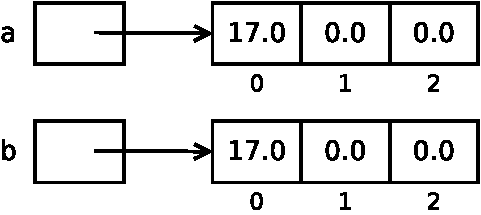
\includegraphics[scale=0.75]{figs/array4.pdf}
\caption{Memory diagram of two variables referring to different arrays.}
\label{fig.array4}
\end{center}
\end{figure}


%\section{Array length}

\index{length!array}
\index{array!length}

The examples so far only work if the array has three elements.
It is better to generalize the code to work with arrays of any size.
We can do that by replacing the magic number, \java{3}, with \java{a.length}:

\begin{code}
double[] b = new double[a.length];
for (int i = 0; i < a.length; i++) {
    b[i] = a[i];
}
\end{code}

All arrays have a built-in constant, \java{length}, that stores the number of elements.
In contrast to \java{String.length()}, which is a method, \java{a.length} is a constant.
The expression \java{a.length} may look like a method invocation, but there are no parentheses and no arguments.

The last time the loop gets executed, \java{i} is \java{a.length - 1}, which is the index of the last element.
When \java{i} is equal to \java{a.length}, the condition fails and the body is not executed -- which is a good thing, because trying to access \java{a[a.length]} would throw an exception.

Of course we can replace the loop altogether by using \java{Arrays.copyOf} and \java{a.length} for the second argument.
The following line produces the same result shown in Figure~\ref{fig.array4}.

\begin{code}
double[] b = Arrays.copyOf(a, a.length);
\end{code}


\section{Array traversal}
\label{traversal}

\index{traversal}

Many computations can be implemented by looping through the elements of an array and performing an operation on each element.
Looping through the elements of an array is called a {\bf traversal}.

\begin{code}
int[] a = {1, 2, 3, 4, 5};
for (int i = 0; i < a.length; i++) {
    a[i] *= a[i];
}
\end{code}

This example traverses an array and squares each element.
At the end of the loop, the array has the values \java{\{1, 4, 9, 16, 25\}}.

\index{search}


Another common pattern is a {\bf search}, which involves traversing an array and ``searching'' for a particular element.
For example, the following method takes an array and a value, and it returns the index where the value appears:

\begin{code}
public static int search(double[] array, double target) {
    for (int i = 0; i < array.length; i++) {
        if (array[i] == target) {
            return i;
        }
    }
    return -1;  // not found
}
\end{code}

If we find the target value in the array, we return its index immediately.
If the loop exits without finding the target, it returns \java{-1}, a special value chosen to indicate a failed search.
(This code is essentially what the \java{String.indexOf} method does.)

The following code searches an array for the value \java{1.23}, which is the third element.
Because array indexes start at zero, the output is \java{2}.

\begin{code}
double[] array = {3.14, -55.0, 1.23, -0.8};
int index = search(array, 1.23);
System.out.println(index);
\end{code}


\index{reduce}

Another common traversal is a {\bf reduce} operation, which ``reduces'' an array of values down to a single value.
Examples include the sum or product of the elements, the minimum, and the maximum.
The following method takes an array and returns the sum of its elements:

\begin{code}
public static double sum(double[] array) {
    double total = 0.0;
    for (int i = 0; i < array.length; i++) {
        total += array[i];
    }
    return total;
}
\end{code}

\index{accumulator}

Before the loop, we initialize \java{total} to zero.
Each time through the loop, we update \java{total} by adding one element from the array.
At the end of the loop, \java{total} contains the sum of the elements.
A variable used this way is sometimes called an {\bf accumulator}, because it ``accumulates'' the running total.


\section{Random numbers}
\label{random}

\index{deterministic}

Most computer programs do the same thing every time they run; programs like that are called {\bf deterministic}.
Usually determinism is a good thing, since we expect the same calculation to yield the same result.
But for some applications, we want the computer to be unpredictable.
Games are an obvious example, but there are many others, like scientific simulations.

%Technically speaking, all computer programs are deterministic: they simply execute the source code.

\index{nondeterministic}
\index{pseudorandom}

Making a program {\bf nondeterministic} turns out to be hard, because it's impossible for a computer to generate truly random numbers.
But there are algorithms that generate unpredictable sequences called {\bf pseudorandom} numbers.
For most applications, they are as good as random.

%Nondeterminism is a theoretical concept for analyzing the complexity of algorithms.

\index{Random}
\index{nextInt!Random}

If you did Exercise~\ref{guess}, you have already seen \java{java.util.Random}, which generates pseudorandom numbers.
The method \java{nextInt} takes an integer argument, \java{n}, and returns a random integer between \java{0} and \java{n - 1} (inclusive).

If you generate a long series of random numbers, every value should appear, at least approximately, the same number of times.
One way to test this behavior of \java{nextInt} is to generate a large number of values, store them in an array, and count the number of times each value occurs.

The following method creates an \java{int} array and fills it with random numbers between 0 and 99.
The argument specifies the desired size of the array, and the return value is a reference to the new array.

\begin{code}
public static int[] randomArray(int size) {
    Random random = new Random();
    int[] a = new int[size];
    for (int i = 0; i < a.length; i++) {
        a[i] = random.nextInt(100);
    }
    return a;
}
\end{code}

The following \java{main} method generates an array and displays it using \java{printArray} from Section~\ref{printarray}.
We could have used \java{Arrays.toString}, but we like seeing curly braces instead of square brackets.

\begin{code}
public static void main(String[] args) {
    int[] array = randomArray(8);
    printArray(array);
}
\end{code}

Each time you run the program, you should get different values.
The output will look something like this:

\begin{stdout}
{15, 62, 46, 74, 67, 52, 51, 10}
\end{stdout}


\section{Building a histogram}
\label{singlepass}

\index{histogram}
\index{counter}

If these values were exam scores -- and they would be pretty bad exam scores in that case -- the teacher might present them to the class in the form of a {\bf histogram}.
In statistics, a histogram is a set of counters that keeps track of the number of times each value appears.

For exam scores, we might have ten counters to keep track of how many students scored in the 90s, the 80s, etc.
To do that, we can traverse the array and count the number of elements that fall in a given range.

The following method takes an array and two integers.
It returns the number of elements that fall in the range from \java{low} to \java{high - 1}.

\begin{code}
public static int inRange(int[] a, int low, int high) {
    int count = 0;
    for (int i = 0; i < a.length; i++) {
        if (a[i] >= low && a[i] < high) {
            count++;
        }
    }
    return count;
}
\end{code}

\index{reduce}

This pattern should look familiar: it is another reduce operation.
Notice that \java{low} is included in the range (\java{>=}), but \java{high} is excluded (\java{<}).
This design keeps us from counting any scores twice.

Now we can count the number of scores in each grade range.
We add the following code to our \java{main} method:

\begin{code}
int[] scores = randomArray(30);
int a = inRange(scores, 90, 100);
int b = inRange(scores, 80, 90);
int c = inRange(scores, 70, 80);
int d = inRange(scores, 60, 70);
int f = inRange(scores, 0, 60);
\end{code}

This code is repetitive, but it is acceptable as long as the number of ranges is small.
Suppose we wanted to keep track of the number of times each individual score appears.
Then we would have to write 100 lines of code:

\begin{code}
int count0 = inRange(scores, 0, 1);
int count1 = inRange(scores, 1, 2);
int count2 = inRange(scores, 2, 3);
...
int count99 = inRange(scores, 99, 100);
\end{code}

What we need is a way to store 100 counters, preferably so we can use an index to access them.
Wait a minute, that's exactly what an array does.

The following fragment creates an array of 100 counters, one for each possible score.
It loops through the scores and uses \java{inRange} to count how many times each score appears.
Then it stores the results in the \java{counts} array:

\begin{code}
int[] counts = new int[100];
for (int i = 0; i < counts.length; i++) {
    counts[i] = inRange(scores, i, i + 1);
}
\end{code}

Notice that we are using the loop variable \java{i} three times: as an index into the \java{counts} array, and in the last two arguments of \java{inRange}.

\index{efficiency}

The code works, but it is not as efficient as it could be.
Every time the loop invokes \java{inRange}, it traverses the entire array.
It would be better to make a single pass through the \java{scores} array.

For each score, we already know which range it falls in -- the score itself.
We can use that value to increment the corresponding counter.
This code traverses the array of scores {\em only once} to generate the histogram:

\begin{code}
int[] counts = new int[100];
for (int i = 0; i < scores.length; i++) {
    int index = scores[i];
    counts[index]++;
}
\end{code}

Each time through the loop, it selects one element from \java{scores} and uses it as an index to increment the corresponding element of \java{counts}.
Because this code traverses the array of scores only once, it is much more efficient.


\section{The enhanced for loop}
\label{enhanced}

Since traversing arrays is so common, Java provides an alternative syntax that makes the code more compact.
Consider a \java{for} loop that displays the elements of an array on separate lines:

\begin{code}
for (int i = 0; i < values.length; i++) {
    int value = values[i];
    System.out.println(value);
}
\end{code}

We could rewrite the loop like this:

\begin{code}
for (int value : values) {
    System.out.println(value);
}
\end{code}

\index{enhanced for loop}
\index{for!enhanced}

This statement is called an {\bf enhanced for loop}, also known as the ``for each'' loop.
You can read the code as, ``for each \java{value} in \java{values}''.
It's conventional to use plural nouns for array variables and singular nouns for element variables.

Notice how the single line \java{for (int value : values)} replaces the first two lines of the standard \java{for} loop.
It hides the details of iterating each index of the array, and instead, focuses on the values themselves.

Using the enhanced \java{for} loop, and removing the temporary variable, we can write the histogram code from the previous section more concisely:

\begin{code}
int[] counts = new int[100];
for (int score : scores) {
    counts[score]++;
}
\end{code}

Enhanced \java{for} loops often make the code more readable, especially for accumulating values.
But they are not helpful when you need to refer to the index, as in search operations.

\begin{code}
for (double d : array) {
    if (d == target) {
        // array contains d, but we don't know where
    }
}
\end{code}


\section{Counting characters}

We now return to the example from the beginning of the chapter and present a solution to Exercise~\ref{doubloon} using arrays.
Here is the problem again:

\begin{quote}
A word is said to be a ``doubloon'' if every letter that appears in the word appears exactly twice.
Write a method called \java{isDoubloon} that takes a string and checks whether it is a doubloon.
To ignore case, invoke the \java{toLowerCase} method before checking.
\end{quote}

Based on the approach from Section~\ref{singlepass}, we will create an array of 26 integers to count how many times each letter appears.
We convert the string to lowercase, so that we can treat \java{'A'} and \java{'a'} (for example) as the same latter.

\begin{code}
int[] counts = new int[26];
String lower = s.toLowerCase();
\end{code}

We can use a \java{for} loop to iterate each character in the string.
To update the \java{counts} array, we need to compute the index that corresponds to each character.
Fortunately, Java allows you to perform arithmetic on characters.

\begin{code}
for (int i = 0; i < lower.length(); i++) {
    char letter = lower.charAt(i);
    int index = letter - 'a';
    counts[index]++;
}
\end{code}

\index{toCharArray}

To simplify the code, it would be nice to use an enhanced \java{for} loop.
The enhanced \java{for} loop does not work with strings directly, but you can convert any string to a character array and iterate that instead:

\begin{code}
for (char letter : lower.toCharArray()) {
    int index = letter - 'a';
    counts[index]++;
}
\end{code}

After counting all the characters in the \java{lower} string, we need one last \java{for} loop to determine whether each letter appears 0 or 2 times.

\begin{code}
for (int count : counts) {
    if (count != 0 && count != 2) {
        return false;  // not a doubloon
    }
}
return true;  // is a doubloon
\end{code}

Like in Section~\ref{traversal}, we can return immediately if the inner condition is true (which, in this example, means that the word is not a doubloon).
If we make it all the way through the \java{for} loop, we know that all counts are 0 or 2.

Pulling together the code fragments, and adding some comments and test cases, here is an entire program.
%This example uses \java{if} statements, \java{for} loops, methods, strings, and arrays.
It's amazing to think about how much you've learned in just seven chapters!

\index{Doubloon.java}

\begin{trinket}{Doubloon.java}
public class Doubloon {

    public static boolean isDoubloon(String s) {
        // count the number of times each letter appears
        int[] counts = new int[26];
        String lower = s.toLowerCase();
        for (char letter : lower.toCharArray()) {
            int index = letter - 'a';
            counts[index]++;
        }
        // determine whether the given word is a doubloon
        for (int count : counts) {
            if (count != 0 && count != 2) {
                return false;
            }
        }
        return true;
    }

    public static void main(String[] args) {
        System.out.println(isDoubloon("Mama"));  // true
        System.out.println(isDoubloon("Lama"));  // false
    }
}
\end{trinket}


\section{Vocabulary}

\begin{description}

\term{array}
A collection of values, where all the values have the same type, and each value is identified by an index.

\term{element}
One of the values in an array.
The \java{[]} operator selects elements.

\term{index}
An integer variable or value used to indicate an element of an array.

\term{allocate}
To reserve memory for an array or other object.
In Java, the \java{new} operator allocates memory.

\term{reference}
A value that indicates a storage location.
In a memory diagram, a reference appears as an arrow.

\term{alias}
A variable that refers to the same object as another variable.

\term{traversal}
Looping through the elements of an array (or other collection).

\term{search}
A traversal pattern used to find a particular element of an array.

\term{reduce}
A traversal pattern that combines the elements of an array into a single value.

\term{accumulator}
A variable used to accumulate results during a traversal.

\term{deterministic}
A program that does the same thing every time it is run.

\term{nondeterministic}
A program that always behaves differently, even when run multiple times with the same input.

\term{pseudorandom}
A sequence of numbers that appear to be random, but which are actually the product of a deterministic computation.

\term{histogram}
An array of integers where each integer counts the number of values that fall into a certain range.

\term{enhanced for loop}
An alternative syntax for traversing the elements of an array (or other collection).

\end{description}


\section{Exercises}

The code for this chapter is in the {\tt ch07} directory of {\tt ThinkJavaCode2}.
See page~\pageref{code} for instructions on how to download the repository.
Before you start the exercises, we recommend that you compile and run the examples.

If you haven't already, take a look at Appendix~\ref{debugging} where we've collected some of our favorite debugging advice.
It refers to language features we haven't yet covered, but it's good for you to know what's available when you need it.


\begin{exercise}  %%V6 Ex8.2

The purpose of this exercise is to practice reading code and recognizing the traversal patterns in this chapter.
The following methods are hard to read, because instead of using meaningful names for the variables and methods, they use names of fruit.

For each method, write one sentence that describes what the method does, without getting into the details of how it works.
And for each variable, identify the role it plays.

\begin{code}
public static int banana(int[] a) {
    int kiwi = 1;
    int i = 0;
    while (i < a.length) {
        kiwi = kiwi * a[i];
        i++;
    }
    return kiwi;
}
\end{code}

\begin{code}
public static int grapefruit(int[] a, int grape) {
    for (int i = 0; i < a.length; i++) {
        if (a[i] == grape) {
            return i;
        }
    }
    return -1;
}
\end{code}

\begin{code}
public static int pineapple(int[] a, int apple) {
    int pear = 0;
    for (int pine: a) {
        if (pine == apple) {
            pear++;
        }
    }
    return pear;
}
\end{code}

\end{exercise}


\begin{exercise}  %%V6 Ex8.3

What is the output of the following program?
Describe in a few words what \java{mus} does.
Draw a stack diagram just before \java{mus} returns.
%that shows the state of the program

\begin{code}
public static int[] make(int n) {
    int[] a = new int[n];
    for (int i = 0; i < n; i++) {
        a[i] = i + 1;
    }
    return a;
}
\end{code}

\begin{code}
public static void dub(int[] jub) {
    for (int i = 0; i < jub.length; i++) {
        jub[i] *= 2;
    }
}
\end{code}

\begin{code}
public static int mus(int[] zoo) {
    int fus = 0;
    for (int i = 0; i < zoo.length; i++) {
        fus += zoo[i];
    }
    return fus;
}
\end{code}

\begin{code}
public static void main(String[] args) {
    int[] bob = make(5);
    dub(bob);
    System.out.println(mus(bob));
}
\end{code}

\end{exercise}


\begin{exercise}  %%V6 Ex8.4

Write a method called \java{indexOfMax} that takes an array of integers and returns the index of the largest element.
Can you write this method using an enhanced \java{for} loop?
Why or why not?

\end{exercise}


\begin{exercise}  %%V6 Ex8.5

The Sieve of Eratosthenes is ``a simple, ancient algorithm for finding all prime numbers up to any given limit,'' which you can read about at \url{https://en.wikipedia.org/wiki/Sieve_of_Eratosthenes}.

Write a method called \java{sieve} that takes an integer parameter, \java{n}, and returns a \java{boolean} array that indicates, for each number from \java{0} to \java{n - 1}, whether the number is prime.

\end{exercise}


\begin{exercise}  %%V6 Ex8.6

Write a method named \java{areFactors} that takes an integer \java{n} and an array of integers, and that returns \java{true} if the numbers in the array are all factors of \java{n} (which is to say that \java{n} is divisible by all of them).

\end{exercise}


\begin{exercise}  %%V6 Ex8.7

Write a method named \java{arePrimeFactors} that takes an integer \java{n} and an array of integers, and that returns \java{true} if the numbers in the array are all prime {\it and} their product is \java{n}.

\end{exercise}


\begin{exercise}  %%V6 Ex9.2

Write a method called \java{letterHist} that takes a string as a parameter and returns a histogram of the letters in the string.
The zeroth element of the histogram should contain the number of a's in the string (upper- and lowercase); the 25th element should contain the number of z's.
Your solution should only traverse the string once.

\end{exercise}


\begin{exercise}  %%V6 Ex9.7

\index{anagram}

Two words are anagrams if they contain the same letters and the same number of each letter.
For example, ``stop'' is an anagram of ``pots'' and ``allen downey'' is an anagram of ``well annoyed''.
Write a method that takes two strings and checks whether they are anagrams of each other.

\end{exercise}


\chapter{Recursive methods}

\index{iterative}
\index{recursive}

Up to this point, we've been using \java{while} and \java{for} loops whenever we've needed to repeat something.
Methods that use iteration are called {\bf iterative}.
They are straight-forward, but sometimes there are more elegant solutions.

In this chapter, we will explore one of the most magical things that a method can do: invoke {\em itself} to solve a smaller version of the {\em same} problem.
A method that invokes itself is called {\bf recursive}.


\section{Recursive void methods}
\label{recursion}

\index{countdown}

Consider the following example:

\begin{code}
public static void countdown(int n) {
    if (n == 0) {
        System.out.println("Blastoff!");
    } else {
        System.out.println(n);
        countdown(n - 1);
    }
}
\end{code}

The name of the method is \java{countdown}; it takes a single integer as a parameter.
If the parameter is zero, it displays the word ``Blastoff''.
Otherwise, it displays the number and then invokes itself, passing \java{n - 1} as the argument.

What happens if we invoke \java{countdown(3)} from \java{main}?

\vspace{-1ex}
\begin{quote}
The execution of \java{countdown} begins with \java{n == 3}, and since \java{n} is not zero, it displays the value 3, and then invokes itself...
\begin{quote}
The execution of \java{countdown} begins with \java{n == 2}, and since \java{n} is not zero, it displays the value 2, and then invokes itself...
\begin{quote}
The execution of \java{countdown} begins with \java{n == 1}, and since \java{n} is not zero, it displays the value 1, and then invokes itself...
\begin{quote}
The execution of \java{countdown} begins with \java{n == 0}, and since \java{n} is zero, it displays the word ``Blastoff!'' and then returns.
\end{quote}
The \java{countdown} that got \java{n == 1} returns.
\end{quote}
The \java{countdown} that got \java{n == 2} returns.
\end{quote}
The \java{countdown} that got \java{n == 3} returns.
\end{quote}
\vspace{-1ex}

And then you're back in \java{main}.
So the total output looks like:

\begin{stdout}
3
2
1
Blastoff!
\end{stdout}

As a second example, we'll rewrite the methods \java{newLine} and \java{threeLine} from Section~\ref{adding_methods}.
Here they are again:

\begin{code}
public static void newLine() {
    System.out.println();
}

public static void threeLine() {
    newLine();
    newLine();
    newLine();
}
\end{code}

\index{newline}

Although these methods work, they would not help if we wanted to display two newlines, or maybe 100.
A more general alternative would be:

\begin{code}
public static void nLines(int n) {
    if (n > 0) {
        System.out.println();
        nLines(n - 1);
    }
}
\end{code}

This method takes an integer, \java{n}, as a parameter and displays \java{n} newlines.
The structure is similar to \java{countdown}.
As long as $n$ is greater than zero, it displays a newline and then invokes itself to display $(n-1)$ additional newlines.
The total number of newlines is $1 + (n - 1)$, which is just what we wanted: $n$.


\section{Recursive stack diagrams}

\index{stack diagram}
\index{diagram!stack}

In the Section~\ref{stack}, we used a stack diagram to represent the state of a program during a method invocation.
The same kind of diagram can make it easier to interpret a recursive method.

Remember that every time a method gets called, Java creates a new frame that contains the current method's parameters and variables.
Figure~\ref{fig.stack2} is a stack diagram for \java{countdown}, called with \java{n == 3}.

\begin{figure}[!ht]
\begin{center}
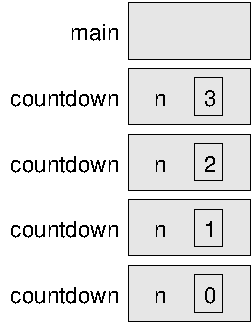
\includegraphics{figs/stack2.pdf}
\caption{Stack diagram for the \java{countdown} program.}
\label{fig.stack2}
\end{center}
\end{figure}

By convention, the frame for \java{main} is at the top, and the stack of other frames grows down.
That way, we can draw stack diagrams on paper without needing to guess how far they will grow.
The frame for \java{main} is empty because \java{main} does not have any variables.
(It has the parameter \java{args}, but since we're not using it, we left it out of the diagram.)

\index{base case}

There are four frames for \java{countdown}, each with a different value for the parameter \java{n}.
The last frame, with \java{n == 0}, is called the {\bf base case}.
It does not make a recursive call, so there are no more frames below it.

\index{StackOverflowError}
\index{exception!StackOverflow}

If there is no base case in a recursive method, or if the base case is never reached, the stack would grow forever -- at least in theory.
In practice, the size of the stack is limited.
If you exceed the limit, you get a \java{StackOverflowError}.

For example, here is a recursive method without a base case:

\begin{code}
public static void forever(String s) {
    System.out.println(s);
    forever(s);
}
\end{code}

\index{call stack}

This method displays the string until the stack overflows, at which point it throws an error.
Try this example on your computer -- you might be surprised by how long the error message is!


\section{Value returning methods}
\label{factorial}

%\index{Turing complete}
%\index{language!complete}
%
%\index{Turing, Alan}
%\index{Church, Alonzo}
%
%Now that we have methods that return values, we have a {\bf Turing complete} programming language.
%That means Java can compute anything computable, for any reasonable definition of ``computable''.
%This idea was developed by Alonzo Church and Alan Turing, so it is known as the Church-Turing thesis.
%You can read more about it at \url{https://en.wikipedia.org/wiki/Turing_thesis}.

To give you an idea of what you can do with the tools we have learned, let's look at methods that evaluate recursively-defined mathematical functions.

A recursive definition is similar to a ``circular'' definition, in the sense that the definition refers to the thing being defined.
Of course, a truly circular definition is not very useful:

\begin{quote}
{\bf recursive:} \\
An adjective used to describe a method that is recursive.
\end{quote}

\index{recursion}

If you saw that definition in the dictionary, you might be annoyed.
Then again, if you search for ``recursion'' on Google, it displays ``Did you mean: recursion'' as an inside joke.
People fall for that link all the time.

\index{factorial}

Many mathematical functions are defined recursively, because that is often the simplest way.
For example, the {\bf factorial} of an integer $n$, which is written $n!$, is defined like this:
%
\begin{eqnarray*}
&&  0! = 1 \\
&&  n! = n \cdot(n-1)!
\end{eqnarray*}
%
Don't confuse the mathematical symbol $!$, which means {\em factorial}, with the Java operator \java{!}, which means {\em not}.
This definition says that \java{factorial(0)} is \java{1}, and that \java{factorial(n)} is \java{n * factorial(n - 1)}.

So \java{factorial(3)} is \java{3 * factorial(2)}; \java{factorial(2)} is \java{2 * factorial(1)}; \java{factorial(1)} is \java{1 * factorial(0)}; and \java{factorial(0)} is \java{1}.
Putting it all together, we get \java{3 * 2 * 1 * 1}, which is 6.

If you can formulate a recursive definition of something, you can easily write a Java method to evaluate it.
The first step is to decide what the parameters and return type are.
Since factorial is defined for integers, the method takes an \java{int} as a parameter and returns an \java{int}.
%So here's a good starting place:

\begin{code}
public static int factorial(int n) {
    return 0;  // stub
}
\end{code}

Next, we think about the base case.
If the argument happens to be zero, we return 1.

\begin{code}
public static int factorial(int n) {
    if (n == 0) {
        return 1;
    }
    return 0;  // stub
}
\end{code}

Otherwise, and this is the interesting part, we have to make a recursive call to find the factorial of $n-1$, and then multiply it by $n$.

\begin{code}
public static int factorial(int n) {
    if (n == 0) {
        return 1;
    }
    int recurse = factorial(n - 1);
    int result = n * recurse;
    return result;
}
\end{code}

To illustrate what is happening, we'll use the temporary variables \java{recurse} and \java{result}.
In each method call, \java{recurse} stores the factorial of $n - 1$, and \java{result} stores the factorial of $n$.

The flow of execution for this program is similar to \java{countdown} from Section~\ref{recursion}.
If we invoke \java{factorial} with the value 3:

\vspace{-1ex}
\begin{quote}
Since 3 is not zero, we skip the first branch and calculate the factorial of $n-1$...
\begin{quote}
Since 2 is not zero, we skip the first branch and calculate the factorial of $n-1$...
\begin{quote}
Since 1 is not zero, we skip the first branch and calculate the factorial of $n-1$...
\begin{quote}
Since 0 {\em is} zero, we take the first branch and return the value 1 immediately.
% without making any more recursive invocations.
\end{quote}
The return value (1) gets multiplied by \java{n}, which is 1, and the result is returned.
\end{quote}
The return value (1) gets multiplied by \java{n}, which is 2, and the result is returned.
\end{quote}
The return value (2) gets multiplied by \java{n}, which is 3, and the result, 6, is returned to whatever invoked \java{factorial(3)}.
\end{quote}
\vspace{-1ex}

\index{stack diagram}
\index{diagram!stack}

Figure~\ref{fig.stack3} shows what the stack diagram looks like for this sequence of method invocations.
The return values are shown being passed up the stack.
Notice that \java{recurse} and \java{result} do not exist in the last frame, because when \java{n == 0} the code that declares them does not execute.

\begin{figure}[!ht]
\begin{center}
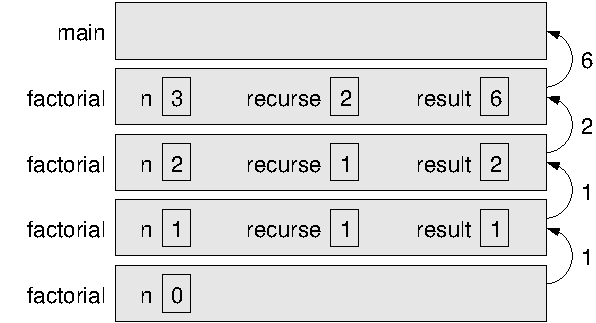
\includegraphics{figs/stack3.pdf}
\caption{Stack diagram for the \java{factorial} method.}
\label{fig.stack3}
\end{center}
\end{figure}


\section{The leap of faith}
\label{leap_of_faith}

\index{leap of faith}

Following the flow of execution is one way to read programs, but it can quickly become overwhelming.
An alternative way to understand recursion is the {\bf leap of faith}:
when you come to a method invocation, instead of following the flow of execution, you {\em assume} that the method works correctly and returns the appropriate value.

In fact, you are already practicing this leap of faith when you use methods in the Java library.
When you invoke \java{Math.cos} or \java{System.out.println}, you don't examine or think about the implementations of those methods.
You just assume that they work properly.

%TODO reference appendix B instead? or use a different example?

For example, this method (from Appendix~\ref{extras}) determines whether an integer has only one digit.
Once you convince yourself that this method is correct -- by testing and examination of the code -- you can use the method without ever looking at the implementation again.

\begin{code}
public static boolean isSingleDigit(int x) {
    return x > -10 && x < 10;
}
\end{code}

The same is true of recursive methods.
When you get to the recursive call, instead of following the flow of execution you should {\em assume} that the recursive invocation works.

For example, ``Assuming that I can find the factorial of $n-1$, can I compute the factorial of $n$?''
Yes you can, by multiplying by $n$.

\begin{code}
public static int factorial(int n) {
    if (n == 0) {
        return 1;
    }
    return n * factorial(n - 1);
}
\end{code}

Notice how similar this implementation (with the temporary variables removed) is to the original mathematical definition.
There is essentially a one-to-one correspondence.
%
\begin{eqnarray*}
&&  0! = 1 \\
&&  n! = n \cdot(n-1)!
\end{eqnarray*}
%
Of course, it is strange to assume that the method works correctly when you have not finished writing it.
But that's why it's called the leap of faith!


\section{Fibonacci sequence}
\label{fibonacci}

\index{fibonacci}

Another common recursively-defined mathematical function is the Fibonacci sequence, which has the following definition:
%
\begin{eqnarray*}
&& fibonacci(1) = 1 \\
&& fibonacci(2) = 1 \\
&& fibonacci(n) = fibonacci(n-1) + fibonacci(n-2)
\end{eqnarray*}
%
Translated into Java, this function is:

\begin{code}
public static int fibonacci(int n) {
    if (n == 1 || n == 2) {
        return 1;
    }
    return fibonacci(n - 1) + fibonacci(n - 2);
}
\end{code}

If you try to follow the flow of execution here, even for small values of \java{n}, your head will explode.
But if we take a leap of faith and assume that the two recursive invocations work correctly, then it is clear, looking at the definition, that our implementation is correct.


\section{Binary number system}

Before introducing the next recursive example, we need to discuss how integers are represented by a computer.

You are probably aware that computers can only store 1's and 0's.
That's because, at the end of the day, processors and memory are made up of billions of tiny on-off switches.

The value 1 means a switch is on; the value 0 means a switch is off.
All types of data, whether integer, floating-point, text, audio, video, or something else, need to be represented by 1's and 0's.

\index{binary}

Fortunately, mathematicians solved this problem centuries ago.
We can represent any integer as a {\bf binary} number.
The following table shows the first eight numbers in binary and decimal (the number system we normally use).

\begin{table}[!ht]
\begin{center}
\begin{tabular}{|c|c|}
\hline
Binary & Decimal \\
\hline
0 & 0 \\
\hline
1 & 1 \\
\hline
10 & 2 \\
\hline
11 & 3 \\
\hline
100 & 4 \\
\hline
101 & 5 \\
\hline
110 & 6 \\
\hline
111 & 7 \\
\hline
\end{tabular}
\caption{The first eight binary numbers.}
\label{tab:binary}
\end{center}
\end{table}

In the decimal system, each part of a number is referred to as a ``digit''.
For example, the number 456 has three digits.
In the binary system, each part of a number is referred to as a ``bit''.
The number 10111 in binary has five bits.

When you hear the phrase ``64-bit computer'', it means that the processors and memory use 64 bits to store integers.
That is where the limits for data types like \java{int} and \java{long} come from.

Decimal numbers are based on powers of 10, because there are 10 possible values for each digit.
For example, the number 456 has 6 in the 1's place, 5 in the 10's place, and 4 in the 100's place.
So the value is 400 + 50 + 6.

\begin{center}
\begin{tabular}{|c|c|c|}
\hline
4 & 5 & 6 \\
\hline
$10^2$ & $10^1$ & $10^0$ \\
\hline
\end{tabular}
\end{center}

Binary numbers are based on powers of 2, because there are 2 possible values for each bit.
For example, the number 10111 has 1 in the 1's place, 1 in the 2's place, 1 in the 4's place, 0 in the 8's place, and 1 in the 16's place.
So the value is 16 + 0 + 4 + 2 + 1, which is 23 in decimal.

\begin{center}
\begin{tabular}{|c|c|c|c|c|}
\hline
1 & 0 & 1 & 1 & 1 \\
\hline
$2^4$ & $2^3$ & $2^2$ & $2^1$ & $2^0$ \\
\hline
\end{tabular}
\end{center}

To convert from decimal to binary, we simply need to divide the number by two repeatedly until we reach zero.
When you divide by two, the remainder will be either 0 or 1.
If you keep track of the remainders, you'll have your binary number.

\begin{stdout}
23 / 2 is 11 remainder 1
11 / 2 is  5 remainder 1
 5 / 2 is  2 remainder 1
 2 / 2 is  1 remainder 0
 1 / 2 is  0 remainder 1
\end{stdout}

Reading these remainders from bottom to top, 23 in binary is 10111.


\section{Recursive binary method}

We can write a recursive method to convert decimal to binary.
Doing so will demonstrate how to compute results in reverse order.

At the start of the chapter, the \java{countdown} example had three parts: (1) it checked the base case, (2) displayed something, and (3) made a recursive call.
What do you think happens if you reverse steps 2 and 3, making the recursive call {\em before} displaying?

\begin{code}
public static void countup(int n) {
    if (n == 0) {
        System.out.println("Blastoff!");
    } else {
        countup(n - 1);
        System.out.println(n);
    }
}
\end{code}

The stack diagram is the same as before, and the method is still called $n$ times.
But now the \java{System.out.println} happens just before each recursive call returns.
As a result, it counts {\em up} instead of down:

\begin{stdout}
Blastoff!
1
2
3
\end{stdout}

We can apply this idea to solve our binary conversion problem.
Here is a recursive method that displays the binary value of any positive integer:

\begin{code}
public static void displayBinary(int value) {
    if (value > 0) {
        displayBinary(value / 2);
        System.out.print(value % 2);
    }
}
\end{code}

If \java{value} is zero, \java{displayBinary} does nothing (that's the base case).
If the argument is positive, the method divides it by two and calls \java{displayBinary} recursively.
When the recursive call returns, the method displays one digit of the result and returns (again).
Figure~\ref{fig.stack4} illustrates this process.

\index{stack diagram}
\index{diagram!stack}

\begin{figure}[!ht]
\begin{center}
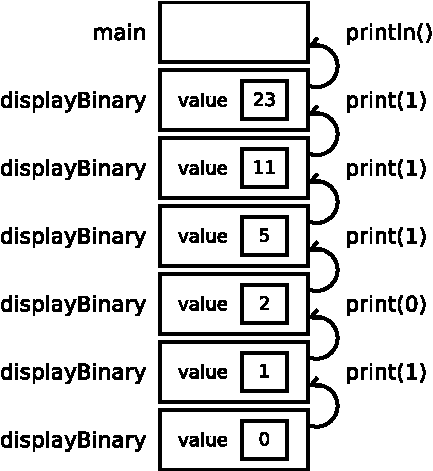
\includegraphics[scale=0.8]{figs/stack4.pdf}
\caption{Stack diagram for the \java{displayBinary} method.}
\label{fig.stack4}
\end{center}
\end{figure}

The leftmost digit is near the bottom of the stack, so it gets displayed first.
The rightmost digit, near the top of the stack, gets displayed last.
After invoking \java{displayBinary}, we use \java{println} to complete the output.

\begin{code}
displayBinary(23);
System.out.println();
// output is 10111
\end{code}


\section{CodingBat problems}

In the past several chapters of this book, you've seen conditions, methods, loops, strings, arrays, and recursion.
A great resource for practicing all of these concepts is \href{http://codingbat.com/java}{\tt CodingBat.com}.

\index{CodingBat}

CodingBat is a free website of live programming problems developed by Nick Parlante, a Computer Science lecturer at Stanford.
As you work on these problems, CodingBat will save your progress (if you create an account).

To conclude this chapter, we will look at two problems in the {\sf Recursion-1} section of CodingBat.
One of them deals with strings, and the other deals with arrays.
Both of them have the same recursive idea: check the base case, look at the current index, and recursively handle the rest.

The first problem is available at \url{http://codingbat.com/prob/p118230}:

\begin{quote}
\textbf{Recursion-1 ~noX}

Given a string, compute recursively a new string where all the 'x' chars have been removed.

\ttfamily
noX("xaxb") $\rightarrow$ "ab" \\
noX("abc") $\rightarrow$ "abc" \\
noX("xx") $\rightarrow$ ""
\end{quote}

When solving recursive problems, it helps to think about the base case first.
The base case is the easiest version of the problem; for noX, it's when you're given the empty string.
If the string is empty, there are no x's to be removed.

\begin{code}
if (str.length() == 0) {
    return "";
}
\end{code}

Next comes the more difficult part.
To solve a problem recursively, you need to think of a simper instance of the same problem.
For noX, it's removing all the x's from a shorter string.

To find an x, we only need to look at one character.
So we can recursively call noX on the rest of the string (the substring at index 1).
Here is the solution:

\begin{code}
char c = str.charAt(0);
if (c == 'x') {
    return noX(str.substring(1));
} else {
    return c + noX(str.substring(1));
}
\end{code}

The \java{else} block ``saves'' the character if it's not an x.
Otherwise, the x is ``removed'' by the first \java{return} statement.

The second problem is available at \url{http://codingbat.com/prob/p135988}:

\begin{quote}
\textbf{Recursion-1 ~array11}

Given an array of ints, compute recursively the number of times that the value 11 appears in the array.

\ttfamily
array11([1, 2, 11], 0) $\rightarrow$ 1 \\
array11([11, 11], 0) $\rightarrow$ 2 \\
array11([1, 2, 3, 4], 0) $\rightarrow$ 0
\end{quote}

This problem uses the convention of passing the index as an argument.
So the base case is when we've reached the end of the array.
At that point, we know there are no more 11's.

\begin{code}
if (index >= nums.length) {
    return 0;
}
\end{code}

Next we look at the current number (based on the given index), and check if it's an 11.
After that, we can recursively check the rest of the array.
Similar to the noX problem, we only look at one integer per method call.

\begin{code}
if (nums[index] == 11) {
    return 1 + array11(nums, index + 1);
} else {
    return array11(nums, index + 1);
}
\end{code}

You can run these solutions on CodingBat by pasting them into the provided method definition.
But don't forget to paste both parts: the base case, and the recursive step.

\index{Java Tutor}

To see how these solutions actually work, you might need to step through them with a debugger (see Appendix~\ref{debugger}) or Java Tutor (\url{http://pythontutor.com/java.html}).
Then try to solve several CodingBat problems of your own.

Learning to think recursively is an important aspect of learning to think like a computer scientist.
Many algorithms can be written concisely with recursive methods that perform computations on the way down, on the way up, or both.


\section{Vocabulary}

\begin{description}

%\term{void method}
%A method that does not return a value.

%\term{value method}
%A method that returns a value.

\term{iterative}
A method or algorithm that repeats steps using one or more loops.

\term{recursive}
A method or algorithm that invokes itself one or more times with different arguments.

%\term{recursion}
%The process of invoking (and restarting) the same method that is currently executing.

\term{base case}
A condition that causes a recursive method {\em not} to make another recursive call.

%\term{Turing complete}
%A programming language that can implement any theoretically possible algorithm.

\term{factorial}
The product of all the integers up to and including a given integer.

\term{leap of faith}
A way to read recursive programs by assuming that the recursive call works, rather than following the flow of execution.

\term{binary}
A system that uses only zeros and ones to represent numbers.
Also known as ``base 2''.

\end{description}


\section{Exercises}

The code for this chapter is in the {\tt ch08} directory of {\tt ThinkJavaCode2}.
See page~\pageref{code} for instructions on how to download the repository.
Before you start the exercises, we recommend that you compile and run the examples.

If you have not already read Appendix~\ref{JUnit}, now might be a good time.
It describes JUnit, a standard framework for writing test code.


\begin{exercise}  %%V6 Ex5.5

The purpose of this exercise is to take a problem and break it into smaller problems, and to solve the smaller problems by writing simple methods.
Consider the first verse of the song ``99 Bottles of Beer'':

\begin{quote}
99 bottles of beer on the wall,\\
99 bottles of beer,\\
ya' take one down, ya' pass it around,\\
98 bottles of beer on the wall.
\end{quote}

Subsequent verses are identical except that the number of bottles gets smaller by one in each verse, until the last verse:

\begin{quote}
No bottles of beer on the wall,\\
no bottles of beer,\\
ya' can't take one down, ya' can't pass it around,\\
'cause there are no more bottles of beer on the wall!
\end{quote}

And then the song (finally) ends.

Write a program that displays the entire lyrics of ``99 Bottles of Beer''.
Your program should include a recursive method that does the hard part, but you might want to write additional methods to separate other parts of the program.
As you develop your code, test it with a small number of verses, like \java{3}.

\end{exercise}


\begin{exercise}  %%V6 Ex6.6

In this exercise, you will use a stack diagram to understand the execution of the following recursive method.

\begin{code}
public static void main(String[] args) {
    System.out.println(prod(1, 4));
}

public static int prod(int m, int n) {
    if (m == n) {
        return n;
    } else {
        int recurse = prod(m, n - 1);
        int result = n * recurse;
        return result;
    }
}
\end{code}

\begin{enumerate}

\item Draw a stack diagram showing the state of the program just before the last invocation of \java{prod} completes.

\item What is the output of this program?
(Try to answer this question on paper first, then run the code to check your answer.)

\item Explain in a few words what \java{prod} does (without getting into the details of how it works).

\item Rewrite \java{prod} without the temporary variables \java{recurse} and \java{result}.
{\it Hint:} You only need one line for the \java{else} branch.

\end{enumerate}

\end{exercise}


\begin{exercise}  %%V6 Ex6.7

Write a recursive method named \java{oddSum} that takes a positive odd integer \java{n} and returns the sum of odd integers from 1 to n.
Start with a base case, and use temporary variables to debug your solution.
You might find it helpful to print the value of \java{n} each time \java{oddSum} is invoked.

\end{exercise}


\begin{exercise}  %%V6 Ex6.8

The goal of this exercise is to translate a recursive definition into a Java method.
The Ackermann function is defined for non-negative integers as follows:
\begin{eqnarray*}
A(m, n) = \begin{cases}
              n+1 & \mbox{if } m = 0 \\
        A(m-1, 1) & \mbox{if } m > 0 \mbox{ and } n = 0 \\
A(m-1, A(m, n-1)) & \mbox{if } m > 0 \mbox{ and } n > 0
\end{cases}
\end{eqnarray*}

Write a recursive method called \java{ack} that takes two \java{int}s as parameters and that computes and returns the value of the Ackermann function.

Test your implementation of Ackermann by invoking it from \java{main} and displaying the return value.
Note the return value gets very big very quickly.
You should try it only for small values of $m$ and $n$ (not bigger than 3).

\end{exercise}


\begin{exercise}  %%V6 Ex6.9
\label{ex.power}

Write a recursive method called \java{power} that takes a double \java{x} and an integer \java{n} and returns $x^n$.

{\it Hint:} A recursive definition of this operation is $x^n = x \cdot x^{n-1}$.
Also, remember that anything raised to the zeroth power is 1.

Optional challenge: you can make this method more efficient, when \java{n} is even, using $x^n = \left( x^{n/2} \right)^2$.

\end{exercise}


\begin{exercise}  %%V6 Ex8.8

Many of the patterns we have seen for traversing arrays can also be written recursively.
It is not common, but it is a useful exercise.

\begin{enumerate}

\item Write a method called \java{maxInRange} that takes an array of integers and two indexes, \java{lowIndex} and \java{highIndex}, and finds the maximum value in the array, but only considering the elements between \java{lowIndex} and \java{highIndex}, including both.

This method should be recursive.
If the length of the range is 1, that is, if \java{lowIndex == highIndex}, we know immediately that the sole element in the range must be the maximum.
So that's the base case.

If there is more than one element in the range, we can break the array into two pieces, find the maximum in each of the pieces, and then find the maximum of the maxima.

\item Methods like \java{maxInRange} can be awkward to use.
To find the largest element in an array, we have to provide the range for the entire array.

\begin{code}
double max = maxInRange(a, 0, a.length - 1);
\end{code}

Write a method called \java{max} that takes an array and uses \java{maxInRange} to find and return the largest element.

\end{enumerate}

\end{exercise}


\begin{exercise}  %%V6 Ex9.4

Create a program called {\tt Recurse.java} and type in the following methods:

\begin{code}
/**
 * Returns the first character of the given String.
 */
public static char first(String s) {
    return s.charAt(0);
}
\end{code}

\begin{code}
/**
 * Returns all but the first letter of the given String.
 */
public static String rest(String s) {
    return s.substring(1);
}
\end{code}

\begin{code}
/**
 * Returns all but the first and last letter of the String.
 */
public static String middle(String s) {
    return s.substring(1, s.length() - 1);
}
\end{code}

\begin{code}
/**
 * Returns the length of the given String.
 */
public static int length(String s) {
    return s.length();
}
\end{code}

\begin{enumerate}

\item Write some code in \java{main} that tests each of these methods.
Make sure they work, and you understand what they do.

\item Using these methods, and without using any other \java{String} methods, write a method called \java{printString} that takes a string as a parameter and that displays the letters of the string, one on each line.
It should be a void method.

\item Again using only these methods, write a method called \java{printBackward} that does the same thing as \java{printString} but that displays the string backward (again, one character per line).

\item Now write a method called \java{reverseString} that takes a string as a parameter and that returns a new string as a return value.
The new string should contain the same letters as the parameter, but in reverse order.

\begin{code}
String backwards = reverseString("coffee");
System.out.println(backwards);
\end{code}

The output of this example code should be:

\begin{stdout}
eeffoc
\end{stdout}

\index{palindrome}

\item A palindrome is a word that reads the same both forward and backward, like ``otto'' and ``palindromeemordnilap''.
Here's one way to test whether a string is a palindrome:

\begin{quotation}
\noindent
A single letter is a palindrome, a two-letter word is a palindrome if the letters are the same, and any other word is a palindrome if the first letter is the same as the last and the middle is a palindrome.
\end{quotation}

Write a recursive method named \java{isPalindrome} that takes a \java{String} and returns a \java{boolean} indicating whether the word is a palindrome.

\end{enumerate}

\end{exercise}


\chapter{Immutable objects}
\label{immutable}

\index{object-oriented}

Java is an ``object-oriented'' language, which means that it uses objects to represent data {\em and} provide methods related to them.
This way of organizing programs is a powerful design concept, and we will introduce it gradually throughout the remainder of the book.

\index{object}
\index{System.in}
\index{System.out}

An {\bf object} is a collection of data that provides a set of methods.
For example, \java{Scanner}, which we saw in Section~\ref{scanner}, is an object that provides methods for parsing input.
\java{System.out} and \java{System.in} are also objects.

Strings are objects, too.
They contain characters and provide methods for manipulating character data.
Other data types, like \java{Integer}, contain numbers and provide methods for manipulating number data.
We will explore some of those methods in this chapter.


\section{Primitives vs objects}

\index{primitive}

Not everything in Java is an object: \java{int}, \java{double}, \java{char}, and \java{boolean} are examples of {\bf primitive} types.
%We will explain some of the differences between object types and primitive types as we go along.
When you declare a variable with a primitive type, Java reserves a small amount of memory to store its value.
Figure~\ref{fig.mem1} shows how the following values are stored memory.

\begin{code}
int number = -2;
char symbol = '!';
\end{code}

\begin{figure}[!ht]
\begin{center}
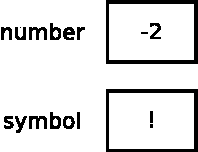
\includegraphics[scale=0.85]{figs/mem1.pdf}
\caption{Memory diagram of two primitive variables.}
\label{fig.mem1}
\end{center}
\end{figure}

\index{memory diagram}
\index{diagram!memory}

As we learned in Section~\ref{elements}, an array variable stores a {\em reference} to an array.
That's because the array itself is too large to fit in the variable's memory.
For example, \java{char[] array = \{'c', 'a', 't'\};} contains three characters.

\begin{figure}[!ht]
\begin{center}
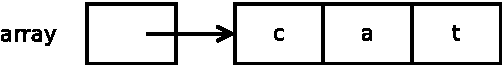
\includegraphics[scale=0.85]{figs/mem2.pdf}
\caption{Memory diagram of an array of characters.}
\label{fig.mem2}
\end{center}
\end{figure}

When drawing memory diagrams, we use an arrow to represent the location of the array, as in Figure~\ref{fig.mem2}.
The actual memory location (the {\em value} of the array variable) is an integer chosen by Java at run-time.

Objects work in a similar way.
When you declare an object variable, it will store a reference to an object.
In contrast to arrays, which store multiple elements of the same data type, objects can be used to {\bf encapsulate} any type of data.
%We will learn more about this concept in Chapter~\ref{mutable}.

For example, a \java{String} object encapsulates a character array.
Figure~\ref{fig.mem3} illustrates how strings are stored in memory.

\begin{figure}[!ht]
\begin{center}
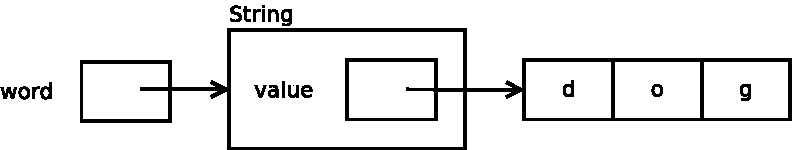
\includegraphics[scale=0.85]{figs/mem3.pdf}
\caption{Memory diagram of a \java{String} object.}
\label{fig.mem3}
\end{center}
\end{figure}

Behind the scenes, the code \java{String word = "dog";} creates an array of the characters \java{'d'}, \java{'o'}, and \java{'g'}, and stores the reference to that array in a \java{String} object.
The variable \java{word} contains a reference to the \java{String} object.

\index{string!comparing}

To test whether two integers (or other primitive types) are equal, you simply use the \java{==} operator.
But as we learned in Section~\ref{strcmp}, you need to use the \java{equals} method to compare strings.
The \java{equals} method traverses the arrays and tests whether they contain the same characters.

On the other hand, two \java{String} objects with the same characters would not be considered equal in the \java{==} sense.
The \java{==} operator, when applied to string variables, only tests whether they refer to the {\em same} object.


%\section{The null keyword}

\index{null}

In Java, the keyword \java{null} is a special value that means ``no object''.
You can initialize object and array variables this way:

\begin{code}
String name = null;
int[] combo = null;
\end{code}

The value \java{null} is represented in memory diagrams by a small box with no arrow, as in Figure~\ref{fig.mem4}.
In other words, the variables do not reference anything.

\begin{figure}[!ht]
\begin{center}
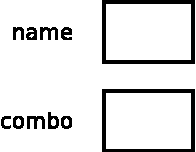
\includegraphics[scale=0.85]{figs/mem4.pdf}
\caption{Memory diagram showing variables that are \java{null}.}
\label{fig.mem4}
\end{center}
\end{figure}

\index{NullPointerException}
\index{exception!NullPointer}

If you try to use a variable that is \java{null} by invoking a method or accessing an element, Java throws a \java{NullPointerException}.

\begin{code}
System.out.println(name.length());  // NullPointerException
System.out.println(combo[0]);       // NullPointerException
\end{code}

On the other hand, it is perfectly fine to pass a \java{null} reference as an argument to a method, or to receive one as a return value.
In these situations, \java{null} is often used to represent a special condition or indicate an error.


\section{Strings are immutable}

If the Java library didn't have a \java{String} class, we would have to use character arrays to store and manipulate text.
Operations like concatenation (\java{+}), \java{indexOf}, and \java{substring} would be difficult and inconvenient.
Fortunately, Java does have a \java{String} class that provides these and other methods.

\index{toUpperCase}
\index{toLowerCase}
\index{immutable}

For example, the methods \java{toLowerCase} and \java{toUpperCase} convert uppercase letters to lowercase, and vice versa.
These methods are often a source of confusion, because it sounds like they modify strings.
But neither these methods nor any others can change a string, because strings are {\bf immutable}.

When you invoke \java{toUpperCase} on a string, you get another \java{String} object as a result.
For example:

\begin{code}
String name = "Alan Turing";
String upperName = name.toUpperCase();
\end{code}

%\index{Turing, Alan}

After these statements run, \java{upperName} refers to the string \java{"ALAN TURING"}.
But \java{name} still refers to \java{"Alan Turing"}.
A common mistake is to assume that \java{toUpperCase} somehow affects the original string:

\begin{code}
String name = "Alan Turing";
name.toUpperCase();           // ignores the return value
System.out.println(name);
\end{code}

The previous code displays \java{"Alan Turing"}, because the value of \java{name} (i.e., the reference to the original \java{String} object) never changes.
If you want to change \java{name} to be uppercase, then you need to assign the return value to it:

\begin{code}
String name = "Alan Turing";
name = name.toUpperCase();    // references the new string
System.out.println(name);
\end{code}

\index{replace}

A similar method is \java{replace}, which finds and replaces instances of one string within another.
This example replaces \java{"Computer Science"} with \java{"CS"}:

\begin{code}
String text = "Computer Science is fun!";
text = text.replace("Computer Science", "CS");
\end{code}

%This example demonstrates a common way to work with string methods.
%It invokes \java{text.replace}, which returns a reference to a new string, \java{"CS is fun!"}.
%Then it assigns the new string to \java{text}, replacing the old string.

As with \java{toUpperCase}, assigning the return value (to \java{text}) is important.
If you don't assign the return value, invoking \java{text.replace} has no effect.

% ABD: Too many new ideas here: the most important one is that you have to do something with the return value. It's not a good time to appreciate the glory of immutability.
% CSM: Now that strings were introduced previously, I would like to make this chapter say more about immutability. But we won't get to the full glory until the next chapter.

Strings are immutable by design, because it simplifies passing them between methods as parameters and return values.
And since the contents of a string can never change, two variables can reference the same string without one accidentally corrupting the other.


\section{Wrapper classes}

Primitive values (like \java{int}s, \java{double}s, and \java{char}s) cannot be \java{null}, and they do not provide methods.
For example, you can't invoke \java{equals} on an \java{int}:

\begin{code}
int i = 5;
System.out.println(i.equals(5));  // compiler error
\end{code}

\index{wrapper class}
\index{class!wrapper}
\index{Character}
\index{Integer}
\index{Double}

But for each primitive type, there is a corresponding {\bf wrapper class} in the Java library.
The wrapper class for \java{int} is named \java{Integer}, with a capital \java{I}.

\begin{code}
Integer i = new Integer(5);
System.out.println(i.equals(5));  // displays true
\end{code}

Other wrapper classes include \java{Boolean}, \java{Character}, \java{Double}, and \java{Long}.
They are in the \java{java.lang} package, so you can use them without importing them.

Like strings, objects from wrapper classes are immutable.
And you need to use the \java{equals} method to compare them.

\begin{code}
Integer x = new Integer(123);
Integer y = new Integer(123);
if (x == y) {                           // false
    System.out.println("x and y are the same object");
}
if (x.equals(y)) {                      // true
    System.out.println("x and y have the same value");
}
\end{code}

Because \java{x} and \java{y} refer to different \java{Integer} objects, the code only displays ``x and y have the same value''.

Each wrapper class defines the constants \java{MIN_VALUE} and \java{MAX_VALUE}.
For example, \java{Integer.MIN_VALUE} is \java{-2147483648}, and \java{Integer.MAX_VALUE} is \java{2147483647}.
Because these constants are available in wrapper classes, you don't have to remember them, and you don't have to write them yourself.

\index{parse}

Wrapper classes also provide methods for converting strings to and from primitive types.
For example, \java{Integer.parseInt} converts a string to (you guessed it) an integer.
In this context, {\bf parse} means ``read and translate''.

\begin{code}
String str = "12345";
int num = Integer.parseInt(str);
\end{code}

The other wrapper classes provide similar methods, like \java{Double.parseDouble} and \java{Boolean.parseBoolean}.
They also each provide \java{toString}, which returns a string representation of a value:

\begin{code}
int num = 12345;
String str = Integer.toString(num);
\end{code}

The result is the string \java{"12345"}, which as you now understand, is stored internally in a character array \java{\{'1', '2', '3', '4', '5'\}}.

\index{NumberFormatException}
\index{exception!NumberFormat}

It's always possible to convert a primitive value to a string, but not the other way around.
The following code throws a \java{NumberFormatException}.

\begin{code}
String str = "five";
int num = Integer.parseInt(str);  // NumberFormatException
\end{code}


\section{Command-line arguments}

\index{args}
\index{command-line interface}

Now that you know about strings, arrays, and wrapper classes, we can {\em finally} explain the \java{args} parameter of the \java{main} method, which we have been ignoring since Chapter~\ref{theway}.
If you are unfamiliar with the command-line interface, please read Appendix~\ref{commandline}.

Let's write a program to find the maximum value in a sequence of numbers.
Rather than read the numbers from \java{System.in} using a \java{Scanner}, we'll pass them as command-line arguments.
Here is a starting point:

\begin{code}
public class Max {
    public static void main(String[] args) {
        System.out.println(Arrays.toString(args));
    }
}
\end{code}

You can run this program from the command line by typing:

\begin{stdout}
java Max
\end{stdout}

\index{empty array}

The output indicates that \java{args} is an {\bf empty array}; that is, it has no elements:

\begin{stdout}
[]
\end{stdout}

If you provide additional values on the command line, they are passed as arguments to \java{main}.
For example, if you run the program like this:

\begin{stdout}
java Max 10 -3 55 0 14
\end{stdout}

The output is:

\begin{stdout}
[10, -3, 55, 0, 14]
\end{stdout}

It's not clear from the output, but the elements of \java{args} are strings.
So \java{args} is the array \java{\{"10", "-3", "55", "0", "14"\}}.
To find the maximum number, we have to convert the arguments to integers.

The following code uses an enhanced \java{for} loop to parse the arguments (using the \java{Integer} wrapper class) and find the largest value:

\begin{code}
int max = Integer.MIN_VALUE;
for (String arg : args) {
    int value = Integer.parseInt(arg);
    if (value > max) {
        max = value;
    }
}
System.out.println("The max is " + max);
\end{code}

We begin by initializing \java{max} to the smallest (most negative) number an \java{int} can represent.
That way, the first value we parse will replace \java{max}.
As we find larger values, they will replace \java{max} as well.

If \java{args} is empty, the result will be \java{MIN_VALUE}.
We can prevent this situation from happening by checking \java{args} at the beginning of the program:

\begin{code}
if (args.length == 0) {
    System.err.println("Usage: java Max <numbers>");
    return;
}
\end{code}

It's customary for programs that require command-line arguments to display a ``usage'' message when there are no arguments given.
For example, if you run {\tt javac} or {\tt java} from the command line without any arguments, you will get a very long message.


\section{BigInteger arithmetic}
% CSM based on text from V6 Exercise 10.4

It might not be clear at this point why you would ever need an integer object when you can just use an \java{int} or \java{long}.
One advantage is the variety of methods that \java{Integer} and \java{Long} provide.
But there is another reason: when you need very large integers that exceed \java{Long.MAX_VALUE}.

\index{BigInteger}

\java{BigInteger} is a Java class that can represent arbitrarily large integers.
There is no upper bound except the limitations of memory size and processing speed.
Take a minute to read the documentation, which you can find by doing a web search for ``Java BigInteger''.

\index{java.math}

To use BigIntegers, you have to \java{import java.math.BigInteger} at the beginning of your program.
There are several ways to create a BigInteger, but the simplest uses \java{valueOf}.
The following code converts a \java{long} to a BigInteger:

\begin{code}
long x = 17;
BigInteger big = BigInteger.valueOf(x);
\end{code}

You can also create BigIntegers from strings.
For example, here is a 20-digit integer that is too big to store using a \java{long}.

\begin{code}
String s = "12345678901234567890";
BigInteger bigger = new BigInteger(s);
\end{code}

Notice the difference in the previous two examples: you use \java{valueOf} to convert integers, and \java{new BigInteger} to convert strings.

Since BigIntegers are not primitive types, the usual math operators don't work.
Instead, we have to use methods like \java{add}.
To add two BigIntegers, we invoke \java{add} on one and pass the other as an argument.

\begin{code}
BigInteger a = BigInteger.valueOf(17);
BigInteger b = BigInteger.valueOf(1700000000);
BigInteger c = a.add(b);
\end{code}

Like strings, \java{BigInteger} objects are immutable.
Methods like \java{add}, \java{multiply}, and \java{pow} all return new BigIntegers, rather than modify an existing one.

Internally, a BigInteger encapsulates an array of \java{int}s, similar to the way a string encapsulates an array of \java{char}s.
Each \java{int} in the array stores a portion of the BigInteger.
The methods of \java{BigInteger} traverse this array to perform addition, multiplication, etc.

For very long floating-point values, take a look at \java{java.math.BigDecimal}.
Interestingly, \java{BigDecimal} objects represent floating-point numbers internally by encapsulating a \java{BigInteger}!


\section{Program development}
\label{encapsulation}

This chapter introduces two main concepts: objects encapsulate other types of data, and they can be designed to be immutable.
Applying these concepts helps us to manage the complexity of programs as they become large.

\index{design process}
\index{encapsulation!and generalization}

Unfortunately, computer science has a lot of overloaded terms.
Another use of the term ``encapsulation'' applies to methods.
In this section, we present a {\bf design process} called ``encapsulation and generalization''.

One challenge of programming, especially for beginners, is figuring out how to divide up a program into methods.
The process of encapsulation and generalization allows you to design as you go along.
The steps are:

\begin{enumerate}
\item Write a few lines of code in \java{main} or another method, and test them.
\item When they are working, wrap them in a new method, and test again.
\item If it's appropriate, replace literal values with variables and parameters.
\end{enumerate}

Encapsulation and generalization is similar to ``incremental development'' (see Section~\ref{distance}), in the sense that you write a little code, test it, and repeat.
But you don't need to begin with an exact method definition and stub.

\index{table!two-dimensional}

To demonstrate this process, we'll develop methods that display multiplication tables.
Here is a loop that displays the multiples of two, all on one line:

\begin{code}
int i = 1;
while (i <= 6) {
    System.out.printf("%4d", 2 * i);
    i = i + 1;
}
System.out.println();
\end{code}

\index{loop variable}
\index{variable!loop}

The first line initializes a variable named \java{i}, which is going to act as the loop variable.
As the loop executes, the value of \java{i} increases from 1 to 6; when \java{i} is 7, the loop terminates.

Each time through the loop, we display the value \java{2 * i} padded with spaces so it's four characters wide.
Since we use \java{System.out.printf}, the output appears on a single line.

After the loop, we call \java{println} to print a newline and complete the line.
Remember that in some environments, none of the output is displayed until the line is complete.

The output of the code so far is:

\begin{stdout}
   2   4   6   8  10  12
\end{stdout}

\index{encapsulate}

The next step is to {\bf encapsulate} or wrap this code in a method.
Here's what it looks like:

\begin{code}
public static void printRow() {
    int i = 1;
    while (i <= 6) {
        System.out.printf("%4d", 2 * i);
        i = i + 1;
    }
    System.out.println();
}
\end{code}

\index{generalize}

Next, we {\bf generalize} the method by replacing the constant value, \java{2}, with a parameter, \java{n}.
This step is called ``generalization'' because it makes the method more general (less specific).

\begin{code}
public static void printRow(int n) {
    int i = 1;
    while (i <= 6) {
        System.out.printf("%4d", n * i);  // generalized n
        i = i + 1;
    }
    System.out.println();
}
\end{code}

Invoking this method with the argument 2 yields the same output as before.
With the argument 3, the output is:

\begin{stdout}
   3   6   9  12  15  18
\end{stdout}

%And with argument 4, the output is:
%
%\begin{stdout}
%   4   8  12  16  20  24
%\end{stdout}

By now you can probably guess how we are going to display a multiplication table: we'll invoke \java{printRow} repeatedly with different arguments.
In fact, we'll use another loop to iterate through the rows.

\begin{code}
int i = 1;
while (i <= 6) {
    printRow(i);
    i = i + 1;
}
\end{code}

And the output looks like this:

\begin{stdout}
   1   2   3   4   5   6
   2   4   6   8  10  12
   3   6   9  12  15  18
   4   8  12  16  20  24
   5  10  15  20  25  30
   6  12  18  24  30  36
\end{stdout}

%The format specifier \java{\%4d} in \java{printRow} causes the output to align vertically, regardless of whether the numbers are one or two digits.


\section{More generalization}

The previous result is similar to the ``nested loops'' approach in Section~\ref{nested}.
However, the inner loop is now encapsulated in the \java{printRow} method.
We can encapsulate the outer loop in a method too:

\begin{code}
public static void printTable() {
    int i = 1;
    while (i <= 6) {
        printRow(i);
        i = i + 1;
    }
}
\end{code}

The initial version of \java{printTable} always displays six rows.
We can generalize it by replacing the literal \java{6} with a parameter:

\begin{code}
public static void printTable(int rows) {
    int i = 1;
    while (i <= rows) {  // generalized rows
        printRow(i);
        i = i + 1;
    }
}
\end{code}

Here is the output of \java{printTable(7)}:

\begin{stdout}
   1   2   3   4   5   6
   2   4   6   8  10  12
   3   6   9  12  15  18
   4   8  12  16  20  24
   5  10  15  20  25  30
   6  12  18  24  30  36
   7  14  21  28  35  42
\end{stdout}

That's better, but it still has a problem: it always displays the same number of columns.
We can generalize more by adding a parameter to \java{printRow}:

\begin{code}
public static void printRow(int n, int cols) {
    int i = 1;
    while (i <= cols) {  // generalized cols
        System.out.printf("%4d", n * i);
        i = i + 1;
    }
    System.out.println();
}
\end{code}

Now \java{printRow} takes two parameters: \java{n} is the value whose multiples should be displayed, and \java{cols} is the number of columns.
Since we added a parameter to \java{printRow}, we also have to change the line in \java{printTable} where it is invoked:

\begin{code}
public static void printTable(int rows) {
    int i = 1;
    while (i <= rows) {
        printRow(i, rows);  // added rows argument
        i = i + 1;
    }
}
\end{code}

When this line executes, it evaluates \java{rows} and passes the value, which is 7 in this example, as an argument.
In \java{printRow}, this value is assigned to \java{cols}.
As a result, the number of columns equals the number of rows, so we get a square 7x7 table (instead of the previous 7x6 table):

%\begin{stdout}
%   1   2   3   4   5   6   7
%   2   4   6   8  10  12  14
%   3   6   9  12  15  18  21
%   4   8  12  16  20  24  28
%   5  10  15  20  25  30  35
%   6  12  18  24  30  36  42
%   7  14  21  28  35  42  49
%\end{stdout}

When you generalize a method appropriately, you often find that it has capabilities you did not plan.
For example, you might notice that the multiplication table is symmetric.
Since $ab = ba$, all the entries in the table appear twice.
You could save ink by printing half of the table, and you would only have to change {\em one line} of \java{printTable}:

\begin{code}
printRow(i, i);  // using i for both n and cols
\end{code}

In English, the length of each row is the same as its row number.
The result is a triangular multiplication table.

\begin{stdout}
   1
   2   4
   3   6   9
   4   8  12  16
   5  10  15  20  25
   6  12  18  24  30  36
   7  14  21  28  35  42  49
\end{stdout}

Generalization makes code more versatile, more likely to be reused, and sometimes easier to write.
In this example, we started with a simple idea and ended with two general-purpose methods.

%Even though the second parameter in \java{printRow} is named \java{size} and we have a variable with the same name, we can still use any value or expression we want for the argument.

%Remember, you do not pass {\em variables} to methods; you pass their current {\em values}.
%In this last example, the value of \java{i} in \java{printTable} is assigned to both \java{n} and \java{cols} in \java{printRow}.


\section{Vocabulary}

\begin{description}

\term{object}
A collection of related data that comes with a set of methods that operate on the data.

\term{primitive}
A data type that stores a single value and provides no methods.

\term{immutable}
An object that, once created, cannot be modified.
Strings are immutable by design.

\term{wrapper class}
Classes in \java{java.lang} that provide constants and methods for working with primitive types.

\term{parse}
To read a string and interpret or translate it.

\term{empty array}
An array with no elements and a length of zero.

\term{design process}
A process for determining what methods a class or program should have.
%So far we have seen ``incremental development'' and ``encapsulation and generalization''.

\term{encapsulate}
To wrap data inside of an object, or to wrap statements inside of a method.

\term{generalize}
To replace something unnecessarily specific (like a constant value) with something appropriately general (like a variable or parameter).

\end{description}


\section{Exercises}

The code for this chapter is in the {\tt ch09} directory of {\tt ThinkJavaCode2}.
See page~\pageref{code} for instructions on how to download the repository.
Before you start the exercises, we recommend that you compile and run the examples.


\begin{exercise}  %%V6 Ex9.1

The point of this exercise is to explore Java types and fill in some of the details that aren't covered in the chapter.

\index{concatenate}

\begin{enumerate}

\item Create a new program named {\tt Test.java} and write a \java{main} method that contains expressions that combine various types using the \java{+} operator.
For example, what happens when you ``add'' a \java{String} and a \java{char}?
Does it perform character addition or string concatenation?
What is the type of the result?
(How can you determine the type of the result?)

\item Make a bigger copy of the following table and fill it in.
At the intersection of each pair of types, you should indicate whether it is legal to use the \java{+} operator with these types, what operation is performed (addition or concatenation), and what the type of the result is.

\begin{center}
\begin{tabular}{|l|l|l|l|l|l|} \hline
        &  boolean  &  ~char~  &  ~~int~~  &  double  &  String \\ \hline
boolean &           &          &           &          &         \\ \hline
char    &           &          &           &          &         \\ \hline
int     &           &          &           &          &         \\ \hline
double  &           &          &           &          &         \\ \hline
String  &           &          &           &          &         \\ \hline
\end{tabular}
\end{center}

\item Think about some of the choices the designers of Java made, based on this table.
How many of the entries seem unavoidable, as if there was no other choice?
How many seem like arbitrary choices from several equally reasonable possibilities?
Which entries seem most problematic?

\item Here's a puzzler: normally, the statement \java{x++} is exactly equivalent to \java{x = x + 1}.
But if \java{x} is a \java{char}, it's not exactly the same!
In that case, \java{x++} is legal, but \java{x = x + 1} causes an error.
Try it out and see what the error message is, then see if you can figure out what is going on.

\item What happens when you add \java{""} (the empty string) to the other types, for example, \java{"" + 5}?

%\item For each data type, what types of values can you assign to it?
%For example, you can assign an \java{int} to a \java{double} but not vice versa.

\end{enumerate}

\end{exercise}


\begin{exercise}  %%V6 Ex8.1

The goal of this exercise is to practice encapsulation and generalization using some of the examples in previous chapters.

\begin{enumerate}

\item Starting with the code in Section~\ref{traversal}, write a method called \java{powArray} that takes a \java{double} array, \java{a}, and returns a new array that contains the elements of \java{a} squared.
Generalize it to take a second argument and raise the elements of \java{a} to the given power.

\item Starting with the code in Section~\ref{enhanced}, write a method called \java{histogram} that takes an \java{int} array of scores from 0 to (but not including) 100, and returns a histogram of 100 counters.
Generalize it to take the number of counters as an argument.

\end{enumerate}

\end{exercise}


\begin{exercise}  %%V6 Ex10.4

\index{factorial}

You might be sick of the factorial method by now, but we're going to do one more version.

\begin{enumerate}

\item Create a new program called {\tt Big.java} and write an iterative version of \java{factorial} (using a \java{for} loop).

\item Display a table of the integers from 0 to 30 along with their factorials.
At some point around 15, you will probably see that the answers are not correct anymore.
Why not?

\item Convert \java{factorial} so that it performs its calculation using BigIntegers and returns a \java{BigInteger} as a result.
You can leave the parameter alone; it will still be an integer.

\item Try displaying the table again with your modified factorial method.
Is it correct up to 30?
How high can you make it go?

\end{enumerate}

\end{exercise}


\begin{exercise}  %%V6 Ex10.5

Many encryption algorithms depend on the ability to raise large integers to a power.
Here is a method that implements an efficient algorithm for integer exponentiation:

\begin{code}
public static int pow(int x, int n) {
    if (n == 0) return 1;

    // find x to the n/2 recursively
    int t = pow(x, n / 2);

    // if n is even, the result is t squared
    // if n is odd, the result is t squared times x
    if (n % 2 == 0) {
        return t * t;
    } else {
        return t * t * x;
    }
}
\end{code}

The problem with this method is that it only works if the result is small enough to be represented by an \java{int}.
Rewrite it so that the result is a \java{BigInteger}.
The parameters should still be integers, though.

You should use the \java{BigInteger} methods \java{add} and \java{multiply}.
But don't use \java{BigInteger.pow}; that would spoil the fun.

\end{exercise}


\begin{exercise}  %%V6 Ex7.5

%The purpose of this exercise is to practice using \java{BigInteger} and \java{BigDecimal}.

One way to calculate $e^x$ is to use the following infinite series expansion.
The $i$th term in the series is $x^i / i!$.
%
\[ e^x = 1 + x + x^2 / 2! + x^3 / 3! + x^4 / 4! + \ldots \]
%
\begin{enumerate}

\item Write a method called \java{myexp} that takes \java{x} and \java{n} as parameters and estimates $e^x$ by adding the first \java{n} terms of this series.
You can use the \java{factorial} method from Section~\ref{factorial} or your iterative version from the previous exercise.

\index{efficiency}

\item You can make this method more efficient by observing that the numerator of each term is the same as its predecessor multiplied by \java{x}, and the denominator is the same as its predecessor multiplied by \java{i}.

Use this observation to eliminate the use of \java{Math.pow} and \java{factorial}, and check that you get the same result.

\item Write a method called \java{check} that takes a parameter, \java{x}, and displays \java{x}, \java{myexp(x)}, and \java{Math.exp(x)}.
The output should look something like:

\begin{stdout}
1.0     2.708333333333333     2.718281828459045
\end{stdout}

You can use the escape sequence \java{"\\t"} to put a tab character between columns of a table.

\item Vary the number of terms in the series (the second argument that \java{check} sends to \java{myexp}) and see the effect on the accuracy of the result.
Adjust this value until the estimated value agrees with the correct answer when \java{x} is 1.

\item Write a loop in \java{main} that invokes \java{check} with the values 0.1, 1.0, 10.0, and 100.0.
How does the accuracy of the result vary as \java{x} varies?
Compare the number of digits of agreement rather than the difference between the actual and estimated values.

\item Add a loop in \java{main} that checks \java{myexp} with the values -0.1, -1.0, -10.0, and -100.0.
Comment on the accuracy.

\end{enumerate}

\end{exercise}


\begin{exercise}  %%V6 Ex9.3

\index{encapsulation}
\index{generalization}

%The purpose of this exercise is to review encapsulation and generalization (see Section~\ref{encapsulation}).
The following code fragment traverses a string and checks whether it has the same number of open and close parentheses:

\begin{code}
String s = "((3 + 7) * 2)";
int count = 0;

for (int i = 0; i < s.length(); i++) {
    char c = s.charAt(i);
    if (c == '(') {
        count++;
    } else if (c == ')') {
        count--;
    }
}

System.out.println(count);
\end{code}

\begin{enumerate}

\item Encapsulate this fragment in a method that takes a string argument and returns the final value of \java{count}.

\item Test your method with multiple strings, including some that are balanced and some that are not.

\item Generalized the code so that it works on any string. What could you do to generalize it more?

\end{enumerate}

\end{exercise}


\chapter{Mutable objects}
\label{mutable}

\index{String class}
\index{type!String}

As you learned in the previous chapter, an object is a collection of data that provides a set of methods.
For example, a \java{String} is a collection of characters that provides methods like \java{charAt} and \java{substring}.

In this chapter, we'll explore two new types of objects: \java{Point} and \java{Rectangle}.
We'll see how to write methods that take objects as parameters and produce objects as return values.

We will also take a first look at the source code for the Java library.


\section{Point objects}
\label{point}

In math, points are often written in parentheses with a comma separating the coordinates.
For example, $(0,0)$ indicates the origin, and $(x,y)$ indicates the point $x$ units to the right and $y$ units up from the origin.

\index{AWT}
\index{java.awt}
\index{Point}
\index{class!Point}

The \java{java.awt} package provides a class named \java{Point} that represents a location in a Cartesian plane.
In order to use the \java{Point} class, you have to import it:

\begin{code}
import java.awt.Point;
\end{code}

\index{new}
\index{operator!new}

Then, to create a new point, you can use the \java{new} operator:

\begin{code}
Point blank;
blank = new Point(3, 4);
\end{code}

\index{declaration}
\index{statement!declaration}
\index{reference}

The first line declares that \java{blank} has type \java{Point}.
The second line creates the new \java{Point} with the given coordinates.
The result of the \java{new} operator is a {\em reference} to the object.
%So \java{blank} contains a reference to the new \java{Point} object.
Figure~\ref{fig.reference} shows the result.

\index{memory diagram}
\index{diagram!memory}

\begin{figure}[!ht]
\begin{center}
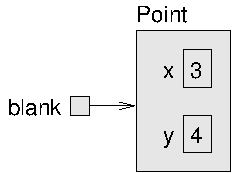
\includegraphics{figs/reference.pdf}
\caption{Memory diagram showing a variable that refers to a \java{Point} object.}
\label{fig.reference}
\end{center}
\end{figure}

As usual, the name of the variable \java{blank} appears outside the box, and its value appears inside the box.
In this case, the value is a reference, which is represented with an arrow.
The arrow points to the \java{Point} object, which contains two variables, \java{x} and \java{y}.


%\section{Attributes}

\index{attribute}
\index{dot notation}

Variables that belong to an object are called {\bf attributes}, but you might also see them referred to as ``fields'' in the documentation.
To access an attribute of an object, Java uses {\bf dot notation}.
For example:

\begin{code}
int x = blank.x;
\end{code}

The expression \java{blank.x} means ``go to the object \java{blank} refers to, and get the value of the attribute \java{x}.''
In this case, we assign that value to a local variable named \java{x}.

There is no conflict between the local variable named \java{x} and the attribute named \java{x}.
The purpose of dot notation is to identify {\em which} variable you are referring to unambiguously.

You can use dot notation as part of an expression.
For example:

\begin{code}
System.out.println(blank.x + ", " + blank.y);
int sum = blank.x * blank.x + blank.y * blank.y;
\end{code}

The first line displays \java{3, 4}.
The second line calculates the value \java{25}.


\section{Objects as parameters}

\index{parameter}
\index{object!as parameter}

You can pass objects as parameters in the usual way.
For example:

\begin{code}
public static void printPoint(Point p) {
    System.out.println("(" + p.x + ", " + p.y + ")");
}
\end{code}

This method takes a point as an argument and displays its attributes in parentheses.
If you invoke \java{printPoint(blank)}, it displays \java{(3, 4)}.

As another example, we can rewrite the \java{distance} method from Section~\ref{distance} so that it takes two \java{Point}s as parameters instead of four \java{double}s.

\begin{code}
public static double distance(Point p1, Point p2) {
    int dx = p2.x - p1.x;
    int dy = p2.y - p1.y;
    return Math.sqrt(dx * dx + dy * dy);
}
\end{code}

Passing objects as parameters makes the source code more readable and less error-prone, because related values are bundled together.

You actually don't need to write a \java{distance} method, because \java{Point} objects have one built-in already.
To compute the distance between two points, we invoke \java{distance} on one and pass the other as an argument.

\begin{code}
Point p1 = new Point(0, 0);
Point p2 = new Point(3, 4);
double dist = p1.distance(p2);  // dist is 5.0
\end{code}

It turns out you don't need the \java{printPoint} method either.
If you invoke \java{System.out.println(blank)} you get even more information:

\begin{stdout}
java.awt.Point[x=3,y=4]
\end{stdout}

\index{toString}

\java{Point} objects provide a method called \java{toString} that returns a string representation of a point.
When you call \java{println} with objects, it automatically calls \java{toString} and displays the result.
In this case, it shows the name of the type (\java{java.awt.Point}) and the names and values of the attributes.


\section{Objects as return types}

\index{Rectangle}
\index{class!Rectangle}

The \java{java.awt} package also provides a class named \java{Rectangle}.
To use it, you have to import it:

\begin{code}
import java.awt.Rectangle;
\end{code}

\java{Rectangle} objects are similar to points, but they have four attributes: \java{x}, \java{y}, \java{width}, and \java{height}.
The following example creates a \java{Rectangle} object and makes the variable \java{box} refer to it:

\begin{code}
Rectangle box = new Rectangle(0, 0, 100, 200);
\end{code}

Figure~\ref{fig.rectangle} shows the effect of this assignment.

\begin{figure}[!ht]
\begin{center}
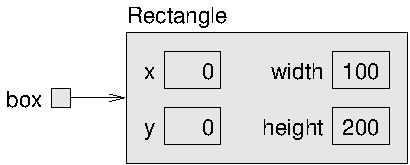
\includegraphics{figs/rectangle.pdf}
\caption{Memory diagram showing a \java{Rectangle} object.}
\label{fig.rectangle}
\end{center}
\end{figure}

If you run \java{System.out.println(box)}, you get:

\begin{stdout}
java.awt.Rectangle[x=0,y=0,width=100,height=200]
\end{stdout}

Again, \java{println} uses the \java{toString} method provided by \java{Rectangle}, which knows how to convert \java{Rectangle} objects into strings.

\index{return}
\index{statement!return}

You can write methods that return new objects.
For example, \java{findCenter} takes a \java{Rectangle} as an argument and returns a \java{Point} with the coordinates of the center of the rectangle:

\begin{code}
public static Point findCenter(Rectangle box) {
    int x = box.x + box.width / 2;
    int y = box.y + box.height / 2;
    return new Point(x, y);
}
\end{code}

The return type of this method is \java{Point}.
The last line creates a new \java{Point} object and returns a reference to it.

\index{coordinate}

You are probably used to Cartesian {\bf coordinates}, where $x$ and $y$ values can be positive or negative.
In contrast, Java uses a coordinate system where the origin is in the upper-left corner.
That way, $x$ and $y$ are always positive integers.
Figure~\ref{fig.coord} shows these coordinate systems side-by-side.

\begin{figure}[!ht]
\begin{center}
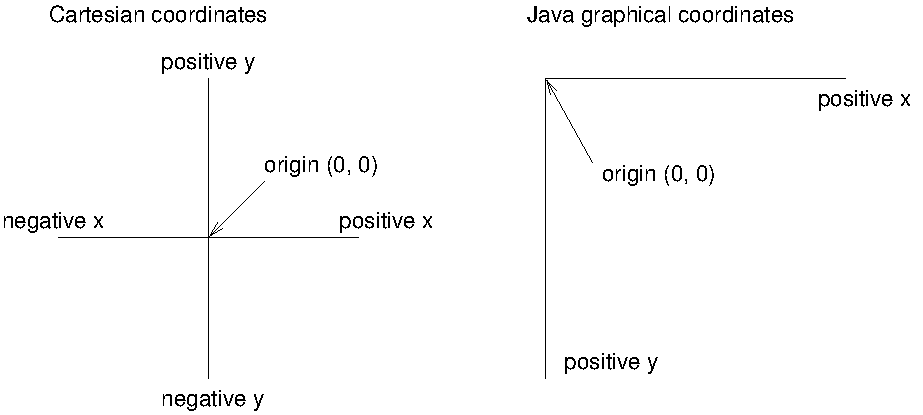
\includegraphics[width=5in]{figs/coordinates.pdf}
\caption{Diagram of the difference between Cartesian coordinates and Java graphical coordinates.}
\label{fig.coord}
\end{center}
\end{figure}

\index{pixel}

Graphical coordinates are measured in {\bf pixels}; each pixel corresponds to a dot on the screen.
You can learn more about Java 2D graphics in Appendix~\ref{graphics}.

The \java{Rectangle} we created using the arguments \java{(0, 0, 100, 200)} has its upper-left corner in the origin.
The center of this rectangle is \java{(50, 100)}, which is 50 pixels to the right and 100 pixels down from the origin.


\section{Rectangles are mutable}

\index{mutable}
\index{object!mutable}

You can change the contents of an object by making an assignment to one of its attributes.
For example, to ``move'' a rectangle without changing its size, you can modify the \java{x} and \java{y} values:

\begin{code}
Rectangle box = new Rectangle(0, 0, 100, 200);
box.x = box.x + 50;
box.y = box.y + 100;
\end{code}

The result is shown in Figure~\ref{fig.rectangle2}.

\begin{figure}[!ht]
\begin{center}
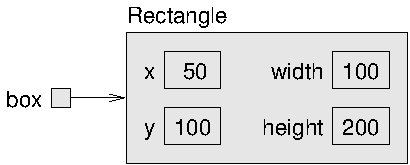
\includegraphics{figs/rectangle2.pdf}
\caption{Memory diagram showing updated attributes.}
\label{fig.rectangle2}
\end{center}
\end{figure}

\index{encapsulation}
\index{generalization}

We can encapsulate this code in a method and generalize it to move the rectangle by any amount:

\begin{code}
public static void moveRect(Rectangle box, int dx, int dy) {
    box.x = box.x + dx;
    box.y = box.y + dy;
}
\end{code}

The variables \java{dx} and \java{dy} indicate how far to move the rectangle in each direction.
Invoking this method has the effect of modifying the \java{Rectangle} that is passed as an argument.

\begin{code}
Rectangle box = new Rectangle(0, 0, 100, 200);
moveRect(box, 50, 100);  // now at (50, 100, 100, 200)
\end{code}

%The code displays \java{java.awt.Rectangle[x=50,y=100,width=100,height=200]}.

Modifying objects by passing them as arguments to methods can be useful.
But it can also make debugging more difficult, because it is not always clear which method invocations modify their arguments.

Java provides a number of methods that operate on \java{Point}s and \java{Rectangle}s.
For example, \java{translate} has the same effect as \java{moveRect}, but instead of passing the rectangle as an argument, you use dot notation:

\begin{code}
box.translate(50, 100);
\end{code}

This line invokes the \java{translate} method for the object that \java{box} refers to.
As a result, the \java{box} object is updated directly.

\index{object-oriented}

This example is a further illustration of {\bf object-oriented} programming.
Rather than write methods like \java{moveRect} that modify one or more parameters, we apply methods to objects themselves using dot notation.


\section{Aliasing revisited}
\label{aliasing}

\index{reference}

Remember that when you assign an object to a variable, you are assigning a {\em reference} to an object.
It is possible to have multiple variables that refer to the same object.
The memory diagram in Figure~\ref{fig.aliasing} shows the result.

\begin{code}
Rectangle box1 = new Rectangle(0, 0, 100, 200);
Rectangle box2 = box1;
\end{code}

\begin{figure}[!ht]
\begin{center}
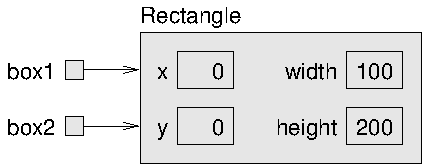
\includegraphics{figs/aliasing.pdf}
\caption{Memory diagram showing two variables that refer to the same \java{Rectangle} object.}
\label{fig.aliasing}
\end{center}
\end{figure}

\index{aliasing}

%Notice how \java{box1} and \java{box2} are aliases for the same object, so any changes that affect one variable also affect the other.

The following example adds 50 to all four sides of the rectangle.
It moves the corner up and to the left by 50, and it increases the height and width by 100:

\begin{code}
System.out.println(box2.width);   // box2.width is 100
box1.grow(50, 50);                // grow box1 (alias)
System.out.println(box2.width);   // box2.width is 200
\end{code}

The first line displays {\tt 100}, which is the width of the \java{Rectangle} referred to by \java{box2}.
The second line invokes the \java{grow} method on \java{box1}, which stretches the \java{Rectangle} horizontally and vertically.
The effect is shown in Figure~\ref{fig.aliasing2}.

\begin{figure}[!ht]
\begin{center}
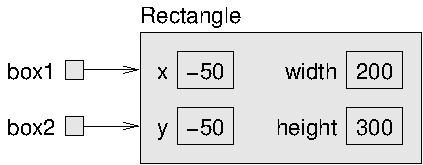
\includegraphics{figs/aliasing2.pdf}
\caption{Memory diagram showing the effect of invoking \java{grow}.}
\label{fig.aliasing2}
\end{center}
\end{figure}

When we make a change using \java{box1}, we see the change using \java{box2}.
Thus, the value displayed by the third line is {\tt 200}, the width of the expanded rectangle.
%(As an aside, it is perfectly legal for the coordinates of a \java{Rectangle} %to be negative.)

%As you can tell from this simple example, code that involves aliasing can get confusing fast, and it can be difficult to debug.
%In general, aliasing should be avoided or used with care.


\section{Java library source}
\label{src.zip}

\index{library}
\index{source code}

Throughout the book, you have used classes from the Java library including \java{System}, \java{String}, \java{Scanner}, \java{Math}, \java{Random}, and others.
You may not have realized that these classes are written in Java.
In fact, you can take a look at the source code to see how they work.

\index{src.zip}

The Java library contains thousands of files, many of which are thousands of lines of code.
That's more than one person could read and understand fully, so don't be intimidated!

Because it's so large, the library source code is stored in a ZIP archive named \java{src.zip}.
Take a few minutes to locate this file on your computer.
In the paths below, you'll need to replace ``\java{...}'' with the version number.

\begin{itemize}
\item On Linux, it's likely under: \verb"/usr/lib/jvm/openjdk-.../"
\\ If not, then install the {\tt openjdk-...-source} package.
\item On MacOS, it's likely under: \\ \verb"/Library/Java/JavaVirtualMachines/jdk.../Contents/Home/"
\item On Windows, it's likely under: \verb"C:\Program Files\Java\jdk...\"
\end{itemize}

When you open (or unzip) the file, you will see folders that correspond to Java packages.
For example, open the {\tt java} folder, and then open the {\tt awt} folder.
You should now see {\tt Point.java} and {\tt Rectangle.java}, along with the other classes in the \java{java.awt} package.

Open {\tt Point.java} in your editor and skim through the file.
It uses language features we haven't yet discussed, so you probably won't understand every single line.
But you can get a sense of what professional Java source code looks like by browsing through the library.

\index{documentation}
\index{HTML}
\index{Javadoc}

Notice how much of {\tt Point.java} is documentation (see Appendix~\ref{javadoc}).
Each method is thoroughly commented, including \java{@param}, \java{@return}, and other tags.
Javadoc reads these comments and generates documentation in HTML.
You can see the results by reading the documentation for the \java{Point} class, which you can find by doing a web search for ``Java Point''.

Now take a look at the \java{Rectangle} class's \java{grow} and \java{translate} methods.
There is more to them than you may have realized, but that doesn't limit your ability to use these methods in a program.
Object-oriented programming makes it possible to hide messy details so that you can more easily use and understand code that other people wrote.

%By looking at the source code for \java{Point}, \java{Rectangle}, and other classes, we hope you will learn two things.
%1) Objects encapsulate data and provide methods to access and modify the data directly.


\section{Class diagrams}
\label{UML}

To summarize what we've learned so far, \java{Point} and \java{Rectangle} objects each have their own attributes and methods.
Attributes are an object's {\em data}, and methods are an object's {\em code}.
An object's {\em class} defines which attributes and methods it will have.

\index{UML}

In practice, it's more convenient to look at high-level pictures than to examine the details of source code.
{\bf Unified Modeling Language} (UML) defines a standard way to summarize the design of a class.

\begin{figure}[!ht]
\begin{center}
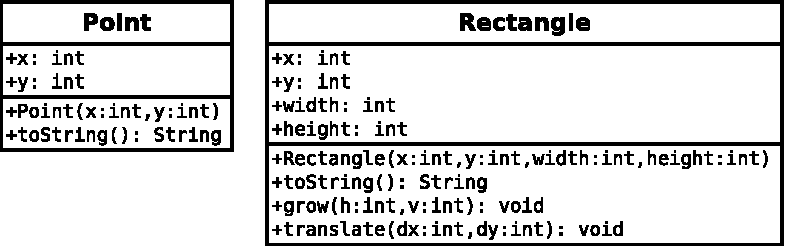
\includegraphics{figs/point-rect.pdf}
\caption{UML class diagrams for \java{Point} and \java{Rectangle}.}
\label{fig.umlPoint}
\end{center}
\end{figure}

\index{class diagram}
\index{diagram!class}

As shown in Figure~\ref{fig.umlPoint}, a {\bf class diagram} is divided into two sections.
The top half lists the attributes, and the bottom half lists the methods.

\index{private}
\index{variable!private}

UML uses a language-independent format, so rather than showing \java{int x}, the diagram uses {\tt x:~int}.
The plus sign (\java{+}) means that the attributes and methods are \java{public}.
%In the case of these two classes, everything is \java{public}.
We'll get to \java{private} attributes (\java{-}) in the next chapter.

In contrast to memory diagrams, which visualize objects (and variables) at run-time, a class diagram visualizes the source code at compile-time.

Both \java{Point} and \java{Rectangle} have additional methods; we are only showing the ones introduced in this chapter.
See the documentation for these classes to learn more about what they can do.


\section{Garbage collection}

In Section~\ref{aliasing}, we saw what happens when more than one variable refers to the same object.
What happens when {\em no} variables refer to an object?

\begin{code}
Point blank = new Point(3, 4);
blank = null;
\end{code}

The first line creates a new \java{Point} object and makes \java{blank} refer to it.
The second line changes \java{blank} so that instead of referring to the object, it refers to nothing.
As shown in Figure~\ref{fig.reference3}, there is no longer an arrow between them.

\begin{figure}[!ht]
\begin{center}
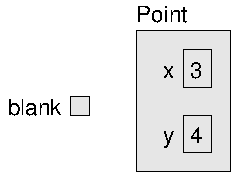
\includegraphics{figs/reference3.pdf}
\caption{Memory diagram showing the effect of setting a variable to \java{null}.}
\label{fig.reference3}
\end{center}
\end{figure}

If there are no references to an object, there is no way to access its attributes or invoke a method on it.
From the program's point of view, it ceases to exist.
However, it's still present in the computer's memory, taking up space.

\index{garbage collection}

As your program runs, the system automatically looks for stranded objects and deletes them; then the space can be reused for new objects.
This process is called {\bf garbage collection}.
%You can manually run the garbage collector by invoking \java{System.gc()} method.

You don't have to do anything to make garbage collection happen, and in general don't have to be aware of it.
But in high-performance applications, you may notice a slight delay every now and then when Java reclaims space from discarded objects.


\section{Mutable vs immutable}

\index{mutable}
\index{immutable}

\java{Point}s and \java{Rectangle}s are {\bf mutable} objects, because their attributes can be modified.
You can modify their attributes directly, like \java{box.x = 15}, or you can invoke methods that modify their attributes, like \java{box.translate(15, 0)}.

In contrast, immutable objects like \java{String}s and \java{Integer}s cannot be modified.
They do not give \java{public} access to their attributes, and they do not provide methods that change their attributes.

Immutable objects have a number of advantages that help improve the performance and reliability of programs.
For example, two strings that contain the same contents can be stored in memory only once.
The Java compiler automatically detects this situation:

\index{Surprise.java}

\begin{trinket}[265]{Surprise.java}
public class Surprise {
    public static void main(String[] args) {
        String s1 = "Hi, Mom!";
        String s2 = "Hi, " + "Mom!";
        if (s1 == s2) {  // true!
            System.out.println("s1 and s2 are the same");
        }
    }
}
\end{trinket}

In this example, \java{s1} and \java{s2} represent the {\em same} string, even though they are created differently.
Because strings are immutable, the compiler decides to reuse a single object for both \java{s1} and \java{s2}.
As a result, \java{s1 == s2}, even though it appears they should be different objects.

Since neither variable can change the string itself, both \java{s1} and \java{s2} will be \java{"Hi, Mom!"} until they are reassigned.
You can pass strings (and other immutable objects) to methods without worrying about their contents changing as a ``side-effect'' of the method.

\index{efficiency}

On the other hand, mutable objects have their own advantages.
It's more efficient to move a rectangle by simply changing its coordinates than to create a brand new \java{Rectangle} each time.
And as we'll see later on, it's easier to implement objects that allow their attributes to be changed.

Strings are particularly inefficient when you need to concatenate them multiple times.
Consider the following program that inputs ten lines from \java{System.in} and concatenates them into a single \java{String}.

\index{Append.java}

\begin{trinket}[325]{Append.java}
import java.util.Scanner;
public class Append {
    public static void main(String[] args) {
        Scanner in = new Scanner(System.in);
        System.out.println("Enter 10 lines:");
        String text = "";
        for (int i = 0; i < 10; i++) {
            String line = in.nextLine();        // new string
            text = text + line + '\n';    // two more strings
        }
        System.out.print("You entered:\n" + text);
    }
}
\end{trinket}

Each time that \java{in.nextLine()} is invoked, it returns a new string.
The next line of code performs \java{text + line}, which creates another string, and then appends the newline character, which creates yet another string.

As a result, the \java{for} loop creates 30 \java{String} objects!
The variable \java{text} references only the most recent \java{String} object.
Garbage collection will delete the other strings, but that's a lot of garbage for a seemly simple program.

The Java library provides the class \java{StringBuilder} for this situation.
It's part of the \java{java.lang} package, so you don't need to import it.
Because \java{StringBuilder} objects are mutable, they can implement concatenation much more efficiently.

All we need to change is the \java{text} variable and the body of the \java{for} loop:

\begin{code}
StringBuilder text = new StringBuilder();
for (int i = 0; i < 10; i++) {
    String line = in.nextLine();
    text.append(line);
    text.append('\n');
}
\end{code}

\java{StringBuilder} provides a number of \java{append} and \java{insert} methods that work with strings efficiently.
It also allows you to \java{delete} portions of a string.


\section{Vocabulary}

\begin{description}

\term{attribute}
One of the named data items that make up an object.
%Each object has its own copy of the attributes for its class.

\term{dot notation}
Use of the dot operator (\java{.}) to access an object's attributes or methods.

\term{coordinate}
A value that specifies a location in a 2D graphical window.

\term{pixel}
The unit in which coordinates are measured.

\term{object-oriented}
A way of organizing code and data into objects, rather than independent methods.

\term{UML}
Unified Modeling Language, a standard way to draw diagrams for software engineering.

\term{class diagram}
An illustration of the attributes and methods for a class.

\term{garbage collection}
The process of finding objects that have no references and reclaiming their storage space.

\term{mutable}
An object that can be modified at any time.
Points and rectangles are mutable by design.

\end{description}


\section{Exercises}

The code for this chapter is in the {\tt ch10} directory of {\tt ThinkJavaCode2}.
See page~\pageref{code} for instructions on how to download the repository.
Before you start the exercises, we recommend that you compile and run the examples.

At this point you know enough to read Appendix~\ref{graphics}, which is about simple 2D graphics and animations.
During the next few chapters, you should take a detour to read this appendix and work through the exercises.


\begin{exercise}  %%V6 Ex10.1

The point of this exercise is to make sure you understand the mechanism for passing objects as parameters.

\begin{enumerate}

\item For the following program, draw a stack diagram showing the local variables and parameters of \java{main} and \java{riddle} just before \java{riddle} returns.
Use arrows to show which objects each variable references.

\item What is the output of the program?

\item Is the \java{blank} object mutable or immutable?
How can you tell?

\end{enumerate}

\begin{code}
public static int riddle(int x, Point p) {
    x = x + 7;
    return x + p.x + p.y;
}
\end{code}

\begin{code}
public static void main(String[] args) {
    int x = 5;
    Point blank = new Point(1, 2);

    System.out.println(riddle(x, blank));
    System.out.println(x);
    System.out.println(blank.x);
    System.out.println(blank.y);
}
\end{code}

\end{exercise}


\begin{exercise}  %%V6 Ex10.2

The point of this exercise is to make sure you understand the mechanism for returning new objects from methods.
The following code uses \java{findCenter} and \java{distance} as defined in this chapter.

\begin{enumerate}

\item Draw a stack diagram showing the state of the program just before \java{findCenter} returns.
Include all variables and parameters, and show the objects those variables refer to.

\item Draw a stack diagram showing the state of the program just before \java{distance} returns.
Show all variables, parameters, and objects.

\item What is the output of this program?
(Can you tell without running it?)

\end{enumerate}

\begin{code}
public static void main(String[] args) {
    Point blank = new Point(5, 8);

    Rectangle rect = new Rectangle(0, 2, 4, 4);
    Point center = findCenter(rect);

    double dist = distance(center, blank);
    System.out.println(dist);
}
\end{code}

\end{exercise}


\begin{exercise}  %%V6 Ex10.3

This exercise is about aliasing.
Recall that aliases are two variables that refer to the same object.
The following code uses \java{findCenter} and \java{printPoint} as defined in this chapter.

\begin{enumerate}

\item Draw a diagram that shows the state of the program just before the end of \java{main}.
Include all local variables and the objects they refer to.

\item What is the output of the program?

\item At the end of \java{main}, are \java{p1} and \java{p2} aliased?
Why or why not?

\end{enumerate}

\begin{code}
public static void main(String[] args) {
    Rectangle box1 = new Rectangle(2, 4, 7, 9);
    Point p1 = findCenter(box1);
    printPoint(p1);

    box1.grow(1, 1);
    Point p2 = findCenter(box1);
    printPoint(p2);
}
\end{code}

\end{exercise}


% Modified on 1/13/05.
\newdimen\snellbaselineskip
\newdimen\snellskip
\snellskip=1.5ex
\snellbaselineskip=\baselineskip
\def\srule{\omit\kern.5em\vrule\kern-.5em}
\newbox\bigstrutbox
\setbox\bigstrutbox=\hbox{\vrule height14.5pt depth9.5pt width0pt}
\def\bigstrut{\relax\ifmmode\copy\bigstrutbox\else\unhcopy\bigstrutbox\fi}
\def\middlehrule#1#2{\noalign{\kern-\snellbaselineskip\kern\snellskip}
&\multispan#1\strut\hrulefill
&\omit\hbox to.5em{\hrulefill}\vrule 
height \snellskip\kern-.5em&\multispan#2\hrulefill\cr}

\makeatletter
\def\bordermatrix#1{\begingroup \m@th
  \@tempdima 8.75\p@
  \setbox\z@\vbox{%
    \def\cr{\crcr\noalign{\kern2\p@\global\let\cr\endline}}%
    \ialign{$##$\hfil\kern2\p@\kern\@tempdima&\thinspace\hfil$##$\hfil
      &&\quad\hfil$##$\hfil\crcr
      \omit\strut\hfil\crcr\noalign{\kern-\snellbaselineskip}%
      #1\crcr\omit\strut\cr}}%
  \setbox\tw@\vbox{\unvcopy\z@\global\setbox\@ne\lastbox}%
  \setbox\tw@\hbox{\unhbox\@ne\unskip\global\setbox\@ne\lastbox}%
  \setbox\tw@\hbox{$\kern\wd\@ne\kern-\@tempdima\left(\kern-\wd\@ne
    \global\setbox\@ne\vbox{\box\@ne\kern2\p@}%
    \vcenter{\kern-\ht\@ne\unvbox\z@\kern-\snellbaselineskip}\,\right)$}%
  \null\;\vbox{\kern\ht\@ne\box\tw@}\endgroup}

\makeatother



%\setcounter{chapter}{9}

\chapter{Markov Chains}\label{chp 11}  

\section{Introduction}\label{sec 11.1}

\par
Most of our study of probability has dealt with independent trials processes. 
These processes are the basis of classical probability theory and much of
statistics.  We have discussed two of the principal theorems for these
processes: the Law of Large Numbers and the Central Limit Theorem.
\par
We have seen that when a sequence of chance experiments forms an independent
trials process, the possible outcomes for each experiment are the same and
occur with the same probability.  Further, knowledge of the outcomes of the
previous experiments does not influence our predictions for the outcomes of the
next experiment.  The distribution for the outcomes of a single experiment is
sufficient to construct a tree and a tree measure for a sequence of $n$
experiments, and we can answer any probability question about these 
experiments by using this tree measure.
\par
Modern probability theory studies chance processes for which the knowledge of
previous outcomes influences predictions for future experiments.  In principle,
when we observe a sequence of chance experiments, all of the past outcomes
could influence our predictions for the next experiment.  For example, this
should be the case in predicting a student's grades on a sequence of exams in a
course.  But to allow this much generality would make it very difficult to
prove general results.
\par
In 1907, A.~A. Markov began the study of an important new type of chance
process.  In this process, the outcome of a given experiment can affect the
outcome of the next experiment.  This type of process is called a Markov
chain.
\subsection*{Specifying a Markov Chain}\index{Markov chain}
We  describe a Markov chain as follows:  We have a set of \emx {states,} $S =
\{s_1,s_2,\ldots,s_r\}$.\index{state!of a Markov chain}  The process starts in
one of 
these states and moves successively from one state to another.  Each
move is called a  \emx {step.}  If the chain is currently in state $s_i$, then
it
moves to state $s_j$ at the next step with a probability denoted by $p_{ij}$,
and this
probability does not depend upon which states the chain was in before the
current state.
\par
The probabilities~$p_{ij}$ are called \emx {transition
probabilities.}\index{transition
probability}\index{probability!transition}  The process can remain in the state
it is in,
and this occurs with probability~$p_{ii}$.  An initial probability
distribution, defined
on~$S$, specifies the starting state.  Usually this is done by specifying a
particular
state as the starting state.

R.~A. Howard\footnote{R.~A. Howard, \emx {Dynamic Probabilistic Systems,}
vol.~1
(New York: John Wiley and Sons, 1971).}\index{HOWARD, R. A.} provides us with a
picturesque
description of a Markov chain as a frog jumping on a set of lily pads. 
The frog starts on one of the pads and then jumps from lily pad to lily
pad with the appropriate transition probabilities.



\begin{example}\label{exam 11.1.1}
According to Kemeny, Snell, and Thompson,\footnote{J.~G. Kemeny, J.~L. Snell,
G.~L. Thompson, \emx {Introduction to Finite Mathematics,} 3rd ed.\ (Englewood
Cliffs, NJ: Prentice-Hall, 1974).}\index{KEMENY, J. G.}\index{SNELL, J.
L.}\index{THOMPSON, G. L.} the Land of Oz\index{Oz, Land of} is blessed by many
things, but
not by good weather.  They never have two nice days in a row.  If they have a
nice day,
they are just as likely to have snow as rain the next day.  If they have snow
or rain, they
have an even chance of having the same the next day.  If there is change from
snow or
rain, only half of the time is this a change to a nice day.  With this
information we form a
Markov chain as follows.  We take as states the kinds of weather R, N, and S. 
From the above information we determine the transition probabilities.  These are most
conveniently represented
in a square array as
$$
\mat {P} = \bordermatrix{
        & \mbox {R} & \mbox {N} & \mbox {S} \cr
\mbox {R} &     1/2 &     1/4 &     1/4 \cr
\mbox {N} &     1/2 &       0 &     1/2 \cr
\mbox {S} &     1/4 &     1/4 &     1/2}\ .
$$
\end{example}

\subsection*{Transition Matrix}
The entries in the first row of the matrix $\mat {P}$ in Example~\ref{exam
11.1.1}
represent  the probabilities for the various kinds of weather following a rainy
day.
Similarly, the entries in the second and third rows represent the probabilities
for
the various kinds of weather following nice and snowy days, respectively.
Such a square array is called the \emx {matrix of transition
probabilities}, or the  \emx {transition matrix}.\index{transition matrix}
\par
We consider the question of determining the probability that, given the chain
is in
state $i$ today, it will be in state $j$ two days from now.  We denote this
probability by $p_{ij}^{(2)}$.  In Example~\ref{exam 11.1.1}, we see that if it
is
rainy today then the event that it is snowy two days from now is the disjoint
union
of the following three events: 1) it is rainy tomorrow and snowy two days from
now,
2) it is nice tomorrow and snowy two days from now, and 3) it is snowy tomorrow
and
snowy two days from now.  The probability of the first of these events is the
product
of the conditional probability that it is rainy tomorrow, given that it is
rainy today,
and the conditional probability that it is snowy two days from now, given that
it is
rainy tomorrow.  Using the transition matrix $\mat{P}$, we can write this
product as
$p_{11}p_{13}$.  The other two events also have probabilities that can be
written as products
of entries of $\mat{P}$.  Thus, we have
$$p_{13}^{(2)} = p_{11}p_{13} + p_{12}p_{23} + p_{13}p_{33}\ .$$
This equation should remind the reader of a dot product of two vectors; we are
dotting the first
row of $ \mat {P}$ with the third column of $ \mat {P}$.  This is just what is
done in
obtaining the $1,3$-entry of the product of $ \mat {P}$ with itself.  
In general, if a Markov chain has $r$ states, then
$$p_{ij}^{(2)} = \sum_{k = 1}^r p_{ik}p_{kj}\ .$$
The following general theorem is easy to prove by using the above observation
and
induction.
\begin{theorem}\label{thm 11.1.1}
Let $ \mat {P}$ be the transition matrix of a Markov chain.  The $ij$th
entry~$p_{ij}^{(n)}$ of the matrix~$ \mat {P}^n$ gives the
probability that the Markov chain, starting in state~$s_i$, will be in
state~$s_j$ after $n$ steps.
\proof
The proof of this theorem is left as an exercise (Exercise~\ref{exer 11.1.18}).
\end{theorem}

\begin{example}\label{exam 11.1.1.5} (Example~\ref{exam 11.1.1} continued)
Consider again the weather in the Land of Oz.  We know that the powers of the
transition matrix give us interesting information about the process as it
evolves.  We shall be particularly interested in the state of the chain after a
large number of steps.  The program {\bf MatrixPowers}\index{MatrixPowers (program)} computes
the powers of~$\mat{P}$.
\par
We have run the program {\bf MatrixPowers} for the Land of Oz example
to compute the successive powers of~$\mat{P}$ from 1~to~6. The results are
shown 
in Table~\ref{table 11.1}.  We note that after six days our weather predictions
are, 
to three-decimal-place accuracy, independent of today's weather.  The
probabilities for the three 
types of weather, R, N, and S, are .4, .2, and .4 no matter where the chain
started.  This is an
example of a type of Markov chain called a \emx {regular} Markov chain.  For
this type of chain,
it is true that long-range predictions are independent of the starting state. 
Not all chains are
regular, but this is an important class of chains that we shall study in detail
later.
\begin{table}
\centering
$$
\mat{P}^1  = \bordermatrix{
            &\mbox{Rain}&\mbox{Nice}&\mbox{Snow} \cr
\mbox{Rain} & .500      & .250      & .250 \cr
\mbox{Nice} & .500      & .000      & .500 \cr
\mbox{Snow} & .250      & .250      & .500 \cr}
$$
$$  
\mat {P}^2  = \bordermatrix{
            &\mbox{Rain}&\mbox{Nice}&\mbox{Snow} \cr
\mbox{Rain} & .438     & .188       & .375 \cr
\mbox{Nice} & .375     & .250       & .375 \cr
\mbox{Snow} & .375     & .188       & .438 \cr}
$$
$$
\mat {P}^3  = \bordermatrix{
            &\mbox{ Rain}&\mbox{Nice} &\mbox{Snow} \cr
\mbox{Rain} & .406       & .203       & .391 \cr
\mbox{Nice} & .406       & .188       & .406 \cr
\mbox{Snow} & .391       & .203       & .406 \cr}
$$
$$  
\mat {P}^4  = \bordermatrix{
            &\mbox{Rain}&\mbox{Nice}&\mbox{Snow} \cr
\mbox{Rain} & .402      & .199      & .398 \cr
\mbox{Nice} & .398      & .203      & .398 \cr
\mbox{Snow} & .398      & .199      & .402 \cr}
$$
$$
\mat {P}^5  = \bordermatrix{
           &\mbox{Rain}&\mbox{Nice}&\mbox{Snow} \cr
\mbox{Rain} & .400     & .200     & .399 \cr
\mbox{Nice} & .400     & .199     & .400 \cr
\mbox{Snow} & .399     & .200     & .400 \cr}
$$
$$  
\mat {P}^6  = \bordermatrix{
           &\mbox{Rain}&\mbox{Nice}&\mbox{Snow} \cr
\mbox{Rain} & .400     & .200     & .400 \cr
\mbox{Nice} & .400     & .200     & .400 \cr
\mbox{Snow} & .400     & .200     & .400 \cr}
$$
\caption{Powers of the Land of Oz transition matrix.}
\label{table 11.1}
\end{table}
\end{example}

We now consider the long-term behavior of a Markov chain when it starts in a
state chosen by a probability distribution
on the set of states, which we will call a \emx {probability
vector}.\index{probability!vector}  A probability vector with $r$ components is
a row
vector whose entries are non-negative and sum to 1.  If $\mat
{u}$ is a probability vector which represents the initial state of a Markov
chain, then we
think of the $i$th component of $\mat {u}$ as representing the probability that
the
chain starts in state $s_i$.
\par
With this interpretation of random starting states, it is easy to prove the
following theorem.
\begin{theorem}\label{thm 11.1.2}
Let $\mat{P}$ be the transition matrix of a Markov chain, and let $\mat {u}$ be
the
probability vector which represents the starting distribution.  Then the
probability
that the chain is in state $s_i$ after $n$ steps is the $i$th entry in the
vector
$$ \mat{u}^{(n)} = \mat{u}{\mat{P}^n}\ .$$
\proof
The proof of this theorem is left as an exercise (Exercise~\ref{exer 11.1.19}).
\end{theorem}

We note that if we want to examine the behavior of the chain under the
assumption
that it starts in a certain state $s_i$, we simply choose $\mat {u}$ to be the
probability vector with $i$th entry equal to 1 and all other entries equal to
0.

\begin{example}\label{exam 11.1.1.6} In the Land of Oz example
(Example~\ref{exam 11.1.1}) let the
initial probability vector $\mat {u}$ equal $(1/3, 1/3, 1/3)$.  Then we can
calculate
the distribution of the states after three days using Theorem~\ref{thm
11.1.2} and our previous calculation of ${\mat {P}^3}$.  We obtain
\begin{eqnarray*}
{\mat {u}}^{(3)} = {\mat {u}}{\mat {P}^3} &=& \pmatrix{ 1/3,& 1/3,& 1/3}
\pmatrix{ .406 & .203 &
.391 \cr   .406 & .188 & .406 \cr .391 & .203 & .406 } \cr
&& \cr
&=& \pmatrix{ .401,& .198,& .401} \ .
\end{eqnarray*}
\end{example}

\subsection*{Examples}
The following examples of Markov chains will be used throughout the chapter for
exercises.

\begin{example}\label{exam 11.1.2}
The President of the United States tells person~A his or her intention to run
or 
not to run in the next election.  Then A relays the news to~B, who in turn
relays 
the message to~C, and so forth, always to some new person.  We assume that
there is
a probability~$a$ that a person will change the answer from yes to no when
transmitting it to the next person and a probability~$b$ that he or she will
change it
from no to yes.  We choose as states the message, either yes or no.  The
transition matrix is then
$$
\mat{P} = \bordermatrix{
           & \mbox{yes} & \mbox{no} \cr
\mbox{yes} &      1 - a &         a \cr
\mbox{no}  &          b &     1 - b}\ .
$$
The initial state represents the President's choice.
\end{example}

\begin{example}\label{exam 11.1.3}
Each time a certain horse runs in a three-horse race, he has probability~1/2 of
winning, 1/4 of coming in second, and 1/4 of coming in third, independent of
the
outcome of any previous race.  We have an independent trials process, but it
can also
be considered from the point of view of Markov chain theory.  The transition
matrix
is
$$
\mat{P} = \bordermatrix{
        & \mbox{W} & \mbox{P} & \mbox{S} \cr
\mbox{W} &      .5 &      .25 &      .25 \cr
\mbox{P} &      .5 &      .25 &      .25 \cr
\mbox{S} &      .5 &      .25 &      .25}\ .
$$
\end{example}
\vskip -3pt
\begin{example}\label{exam 11.1.4}
In the Dark Ages, Harvard, Dartmouth, and Yale admitted only male students. 
Assume that, at that time, 80~percent of the sons of Harvard men went to
Harvard
and the rest went to Yale, 40~percent of the sons of Yale men went to Yale, and
the rest split evenly between Harvard and Dartmouth; and of the sons of
Dartmouth men, 70~percent went to Dartmouth, 20~percent to Harvard, and
10~percent to Yale.  We form a Markov chain with transition matrix
$$
\mat{P} = \bordermatrix{
        & \mbox{H} & \mbox{Y} & \mbox{D} \cr
\mbox{H} &      .8 &      .2 &       0 \cr
\mbox{Y} &      .3 &      .4 &      .3 \cr 
\mbox{D} &      .2 &      .1 &      .7}\ .
$$
\end{example}
\vskip -3pt
\begin{example}\label{exam 11.1.5}
Modify Example~\ref{exam 11.1.4} by assuming that the son of a Harvard man
always went
to Harvard.  The transition matrix is now
$$
\mat{P} = \bordermatrix{
        & \mbox{H} & \mbox{Y} & \mbox{D} \cr
\mbox{H} &       1 &       0 &       0 \cr
\mbox{Y} &      .3 &      .4 &      .3 \cr
\mbox{D} &      .2 &      .1 &      .7}\ .
$$
\end{example}
\vskip -3pt
\begin{example}\label{exam 11.1.6}\index{Ehrenfest model}
\index{gas diffusion!Ehrenfest model of}
(Ehrenfest Model) The following is a special case of a model, called the
Ehrenfest
model,\footnote{P. and T. Ehrenfest, ``\"{U}ber zwei bekannte Einw\"{a}nde
gegen das
Boltzmannsche  H-Theorem," \emx {Physikalishce Zeitschrift,} vol.~8 (1907),
pp.~311-314.}\index{EHRENFEST, P.}
\index{EHRENFEST, T}
that has been used to explain diffusion of gases.  The general model will be
discussed in detail in Section~\ref{sec 11.5}.  We have two urns that, between
them,
contain four balls.  At each step, one of the four balls is chosen at random
and
moved from the urn that it is in into the other urn.  We choose, as states, the
number of balls in the first urn.  The transition matrix is then
$$
 \mat {P} = \bordermatrix{
  &  0  &  1  &  2  &  3  &  4  \cr
0 &  0  &  1  &  0  &  0  &  0  \cr
1 & 1/4 &  0  & 3/4 &  0  &  0  \cr
2 &  0  & 1/2 &  0  & 1/2 &  0  \cr
3 &  0  &  0  & 3/4 &  0  & 1/4 \cr
4 &  0  &  0  &  0  &  1  &  0 \cr}\ . 
$$
\end{example}

\begin{example}\label{exam 11.1.7}\index{genes}
(Gene Model) The simplest type of inheritance of traits in animals occurs when
a trait is
governed by a pair of genes, each of which may be of two types, say G~and~g. 
An individual may have a GG combination or Gg (which is genetically the same as
gG) or gg.  Very often the GG and Gg types are indistinguishable in appearance,
and then we say that the G~gene dominates the g~gene.  An individual is called
 \emx {dominant} if he or she has GG~genes, \emx {recessive} if he or she has
gg, and \emx {hybrid} with a Gg mixture.
\par
In the mating of two animals, the offspring inherits one gene of the pair from
each parent, and the basic assumption of genetics is that these genes are
selected at random, independently of each other.  This assumption determines
the probability of occurrence of each type of offspring.  The offspring of two
purely dominant parents must be dominant, of two recessive parents must be
recessive, and of one dominant and one recessive parent must be hybrid.
\par
In the mating of a dominant and a hybrid animal, each offspring must get a
G~gene from the former and has an equal chance of getting G~or~g from the
latter.  Hence there is an equal probability for getting a dominant or a hybrid
offspring.  Again, in the mating of a recessive and a hybrid, there is an even
chance for getting either a recessive or a hybrid.  In the mating of two
hybrids, the offspring has an equal chance of getting G~or~g from each parent. 
Hence the probabilities are 1/4 for GG, 1/2 for Gg, and 1/4 for gg.
\par
Consider a process of continued matings.  We start with an individual of
known genetic character and mate it with a hybrid.  We assume that there is at
least
one offspring.  An offspring is chosen at random and is mated with a hybrid and
this process
repeated through a number of generations.  The genetic type of the chosen
offspring in
successive generations can be represented by a Markov chain.  The states are
dominant, hybrid, and recessive, and indicated by GG, Gg, and gg respectively.
\par
The transition probabilities are
$$
\mat{P} = \bordermatrix{
          &\mbox{GG} & \mbox{Gg} & \mbox{gg} \cr
\mbox{GG} &  .5      & .5        &   0       \cr
\mbox{Gg} & .25      & .5        & .25       \cr
\mbox{gg} &   0      & .5        &  .5       }\ . 
$$
\end{example}

\begin{example}\label{exam 11.1.8}
Modify Example~\ref{exam 11.1.7} as follows:  Instead of mating the oldest
offspring with a hybrid, we mate it with a dominant individual.  The transition
matrix
is
$$
\mat{P} = \bordermatrix{
   & \mbox{GG} & \mbox{Gg} &\mbox{gg} \cr
\mbox{GG} &  1 &  0 &  0 \cr
\mbox{Gg} & .5 & .5 &  0 \cr
\mbox{gg} &  0 &  1 &  0}\ .
$$
\end{example}

\begin{example}\label{exam 11.1.9}
We start with two animals of opposite sex, mate them, select two of their
offspring of opposite sex, and mate those, and so forth.  To simplify the
example, we will assume that the trait under consideration is independent of
sex.
\par
Here a state is determined by a pair of animals.  Hence, the states of our
process will be: $s_1 = (\mbox{GG},\mbox{GG})$, $s_2 = (\mbox{GG},\mbox{Gg})$,
$s_3 = (\mbox{GG},\mbox{gg})$, $s_4 = (\mbox{Gg},\mbox{Gg})$, $s_5 =
(\mbox{Gg},\mbox{gg})$, and $s_6 = (\mbox{gg},\mbox{gg})$.
\par
We illustrate the calculation of transition probabilities in terms of the
state~$s_2$.  When the process is in this state, one parent has GG~genes, the
other Gg.  Hence, the probability of a dominant offspring is~1/2.  Then the
probability of transition to~$s_1$ (selection of two dominants) is~1/4,
transition to~$s_2$ is~1/2, and to~$s_4$ is~1/4.  The other states are treated
the same way.  The transition matrix of this chain is:  
\par

$$
{\mat{P}^1} = \bordermatrix{            
&\mbox{GG,GG}&\mbox{GG,Gg}&\mbox{GG,gg}&\mbox{Gg,Gg}&\mbox{Gg,gg}&\mbox{gg,gg}\cr
\mbox{GG,GG} & 1.000 & .000 &  .000 &  .000 &  .000 &  .000\cr
\mbox{GG,Gg} &  .250 & .500 &  .000 &  .250 &  .000 &  .000\cr
\mbox{GG,gg} &  .000 & .000 &  .000 & 1.000 &  .000 &  .000\cr
\mbox{Gg,Gg} &  .062 & .250 &  .125 &  .250 &  .250 &  .062\cr
\mbox{Gg,gg} &  .000 & .000 &  .000 &  .250 &  .500 &  .250\cr
\mbox{gg,gg} &  .000 & .000 &  .000 &  .000 &  .000 &  1.000}\ .
$$
 
\end{example}

\begin{example} \label{exam 11.1.10}\index{stepping stones}
(Stepping Stone Model)  Our final example is another example that has been used
in the
study of genetics.  It is called the \emx {stepping stone} model.\footnote{S.
Sawyer, ``Results for The Stepping Stone Model for Migration in Population
Genetics," \emx {Annals of Probability,} vol.~4 (1979),
pp.~699--728.}\index{SAWYER, S.}  In this
model we have an $n$-by-$n$ array of squares, and each square is initially any
one of $k$ different colors.  For each step, a square is chosen at random. 
This
square then chooses one of its eight neighbors at random and assumes the color
of that neighbor.  To avoid boundary problems, we assume that if a square $S$
is on the
left-hand boundary, say, but not at a corner, it is adjacent to the square $T$
on the
right-hand boundary in the same row as $S$, and $S$ is also adjacent to the
squares
just above and below $T$.  A similar assumption is made about squares on the
upper and
lower boundaries.  The top left-hand corner square is adjacent to three obvious neighbors, namely the squares below it,  to its right, and diagonally below and to the right.  It has five other neighbors, which are as follows:  the other three corner squares, the square below the upper right-hand corner, and the square to the right of the bottom left-hand corner.  The other three corners also have, in a similar way, eight neighbors.  (These adjacencies are much easier to understand if one
imagines
making the array into a cylinder by gluing the top and bottom edge together,
and then
making the cylinder into a doughnut by gluing the two circular boundaries
together.) 
With these adjacencies, each square in the array is adjacent to exactly eight
other
squares.
\par
A state in this Markov chain is a description of the color of
each square.  For this Markov chain the number of states is~$k^{n^2}$, which
for
even a small array of squares is enormous.  This is an example of a Markov
chain that is easy to simulate but difficult to analyze in terms of its
transition matrix.  The program {\bf SteppingStone}\index{SteppingStone (program)} simulates
this chain.  We have started with a random initial configuration of two colors
with $n = 20$ and show the result after the process has run for some time in
Figure~\ref{fig 11.2}.
\noindent
\par
This is an example of an \emx {absorbing} Markov chain.  This type of chain
will be studied in
Section~\ref{sec 11.2}.  One of the theorems proved in that section, applied to
the present
example, implies that with
probability 1, the stones will eventually all be the same color.  By watching
the program run, you
can see that territories are established and a battle develops to see which
color survives.  At
any time the probability that a particular color will win out is equal to the
proportion of the
array of this color.  You are asked to prove this in Exercise~\ref{sec
11.2}.\ref{exer 11.2.31}.
\end{example}

\putfig{2truein}{PSfig11-1}{Initial state of the stepping stone model.}{fig 11.1}

%\begin{figure}
%\centerline{\epsfxsize=2truein 
%\epsffile{PSfig11-1}}
%\caption{Initial state of the stepping stone model.}\label{fig 11.1}
%\end{figure}
\nopagebreak[4]
\putfig{2truein}{PSfig11-2}{State of the stepping stone model after 10,000 steps.}{fig 11.2}

%\begin{figure}
%\centerline{\epsfxsize=2truein 
%\epsffile{PSfig11-2}}
%\caption{State of the stepping stone model after 10,000 steps.}\label{fig 11.2}
%\end{figure}

\exercises
\begin{LJSItem}

\i\label{exer 11.1.1} It is raining in the Land of Oz.  Determine a tree and a
tree 
measure for the next three days' weather.  Find $\mat {w}^{(1)},  \mat
{w}^{(2)},$ and
$ \mat {w}^{(3)}$ and compare with the results obtained from $ \mat {P},~\mat
{P}^2,$ 
and~$ \mat {P}^3$.

\i\label{exer 11.1.2} In Example~\ref{exam 11.1.2}, let $a = 0$ and $b = 1/2$. 
Find 
$ \mat {P},~ \mat {P}^2,$ and $ \mat {P}^3.$  What would $ \mat {P}^n$ be? 
What happens 
to~$ \mat {P}^n$ as $n$ tends to infinity?  Interpret this result.

\i\label{exer 11.1.3} In Example~\ref{exam 11.1.3}, find $\mat{P}$,~$ \mat
{P}^2,$
and~$ \mat {P}^3.$  What is $ \mat {P}^n$?

\i\label{exer 11.1.4} For Example~\ref{exam 11.1.4}, find the probability that
the 
grandson of a man from Harvard went to Harvard.

\i\label{exer 11.1.5} In Example~\ref{exam 11.1.5}, find the probability that
the 
grandson of a man from Harvard went to Harvard.

\i\label{exer 11.1.6} In Example~\ref{exam 11.1.7}, assume that we start with a
hybrid 
bred to a hybrid.  Find $ \mat {u}^{(1)},$~$ \mat {u}^{(2)},$ and~$ \mat
{u}^{(3)}.$  
What would $ \mat {u}^{(n)}$ be?

\i\label{exer 11.1.7} Find the matrices $\mat{ P}^2,~\mat {P}^3,~\mat {P}^4,$ 
and~$ \mat {P}^n$ for the Markov chain determined by the transition matrix $
\mat {P} = 
\pmatrix{ 1 & 0 \cr 0 & 1 \cr}$.  Do the same for the transition matrix $ \mat
{P} =
\pmatrix{ 0 & 1 \cr 1 & 0 \cr}$.  Interpret what happens in each of these
processes.

\i\label{exer 11.1.8} A certain calculating machine uses only the digits
0~and~1.  It is supposed to transmit one of these digits through several
stages.  However, at every stage, there is a probability~$p$ that the digit
that
enters this stage will be changed when it leaves and a probability $q = 1 - p$
that it won't.  Form a Markov chain to represent the process of transmission by
taking as states the digits 0~and~1.  What is the matrix of transition
probabilities?

\i\label{exer 11.1.9} For the Markov chain in Exercise~\ref{exer 11.1.8}, draw
a tree 
and assign a tree measure assuming that the process begins in state~0 and moves
through
two stages of transmission.  What is the probability that the machine, after
two
stages, produces the digit~0 (i.e., the correct digit)?  What is the
probability that the machine never changed the digit from~0?  Now let $p = .1$. 
Using
the program {\bf MatrixPowers}, compute the 100th power of the transition
matrix.
Interpret the entries of this matrix.  Repeat this with $p = .2$.  Why do the
100th
powers appear to be the same?

\i\label{exer 11.1.10} Modify the program {\bf MatrixPowers} so that it prints
out
the average $ \mat {A}_n$ of the powers $\mat {P}^n$, for $n = 1$ to $N$.
Try your program on the Land of Oz example and compare $\mat {A}_n$~and~$\mat
{P}^n.$

\i\label{exer 11.1.11} Assume that a man's profession can be classified as
professional, skilled laborer, or unskilled laborer.  Assume that, of the sons
of professional men, 80~percent are professional, 10~percent are skilled
laborers, and 10~percent are unskilled laborers.  In the case of sons of
skilled laborers, 60~percent are skilled laborers, 20~percent are professional,
and 20~percent are unskilled.  Finally, in the case of unskilled laborers,
50~percent of the sons are unskilled laborers, and 25~percent each are in the
other two categories.  Assume that every man has at least one son, and form a
Markov chain
by following the profession of a randomly chosen son of a given family through
several generations.  Set up the matrix of transition probabilities.  Find the
probability that a randomly chosen grandson of an unskilled laborer is a
professional man.

\i\label{exer 11.1.12} In Exercise~\ref{exer 11.1.11}, we assumed that every
man has 
a son.  Assume instead that the probability that a man has at least one son
is~.8.  
Form a Markov chain with four states.  If a man has a son, the probability that
this
son is in a particular profession is the same as in Exercise~\ref{exer
11.1.11}.  If
there is no son, the process moves to state four which represents families
whose male line has died out.  Find the matrix of transition probabilities and
find the probability that a randomly chosen grandson of an unskilled laborer is
a
professional man.

\i\label{exer 11.1.14} Write a program to compute $\mat {u}^{(n)}$ given $\mat
{u}$ and 
$\mat{P}$.  Use this program to compute $\mat {u}^{(10)}$ for the Land of Oz
example, with 
$\mat {u} = (0, 1, 0)$, and with $\mat {u} = (1/3, 1/3, 1/3)$.

\i\label{exer 11.1.15} Using the program {\bf  MatrixPowers}, find $\mat {P}^1$
through 
$\mat {P}^6$ for Examples~\ref{exam 11.1.7} and \ref{exam 11.1.8}.  See if you
can 
predict the long-range probability of finding the process in each of the states
for 
these examples.

\i\label{exer 11.1.16} Write a program to simulate the outcomes of a Markov
chain after $n$~steps, given the initial starting state and the transition
matrix $\mat{P}$ as data (see Example~\ref{exam 11.1.10}).  Keep this program
for use in
later problems.

\i\label{exer 11.1.17} Modify the program of Exercise~\ref{exer 11.1.16} so
that it 
keeps track of the proportion of times in each state in $n$~steps.  Run the
modified
program for different starting states for Example~\ref{exam 11.1.1} and 
Example~\ref{exam 11.1.6}.  Does the initial state affect the proportion of
time 
spent in each of the states if $n$ is large?

\i\label{exer 11.1.18} Prove Theorem~\ref{thm 11.1.1}.

\i\label{exer 11.1.19} Prove Theorem~\ref{thm 11.1.2}.

\i\label{exer 11.1.20} Consider the following process.  We have two coins, one
of which
is fair, and the other of which has heads on both sides.   We give these two
coins to
our friend, who chooses one of them at random (each with probability 1/2). 
During the
rest of the process, she uses only the coin that she chose.  She now proceeds
to toss
the coin many times, reporting the results.  We consider this process to
consist solely of
what she reports to us.
\begin{enumerate}
\item Given that she reports a head on the $n$th toss, what is the probability
that
a head is thrown on the $(n+1)$st toss?

\item Consider this process as having two states, heads and tails.  By
computing the
other three transition probabilities analogous to the one in part (a), write
down a 
``transition matrix" for this process.

\item Now assume that the process is in state ``heads" on both the $(n-1)$st
and the
$n$th toss.  Find the probability that a head comes up on the $(n+1)$st toss.

\item Is this process a Markov chain?
\end{enumerate}

\end{LJSItem}

\section{Absorbing Markov Chains}\label{sec 11.2}
The subject of Markov chains is best studied by considering special types of
Markov chains.  The first type that we shall study is called an \emx {absorbing
Markov chain.}\index{Markov chain!absorbing}\index{absorbing Markov chain}
\begin{definition}
A state~$s_i$ of a Markov chain is called \emx
{absorbing}\index{state!absorbing}\index{absorbing state} if it is impossible
to leave
it (i.e.,
$p_{ii} = 1$).  A Markov chain is \emx {absorbing} if it has at least one
absorbing
state, and if from every state it is possible to go to an absorbing state (not
necessarily
in one step).
\end{definition}
\begin{definition}
In an absorbing Markov chain, a state which is not absorbing is
called \emx{transient.}\index{state!transient}\index{transient state}
\end{definition}

\subsection*{Drunkard's Walk}\index{Drunkard's Walk example}
\begin{example}\label{exam 11.2.1}
A man walks along a four-block stretch of Park Avenue (see Figure~\ref{fig
11.3}).  If he is
at corner 1, 2, or 3, then he walks to the left or right with equal
probability.
He continues until he reaches
corner~4, which is a bar, or corner~0, which is his home.  If he
reaches either home or the bar, he stays there.

\par
We form a Markov chain with states 0,~1, 2, 3, and~4.  States 0~and~4 are
absorbing states.  The transition matrix is then

$$
\mat{P} =\bordermatrix{
  &  0  &  1  &  2  &  3  &  4  \cr
0 &  1  &  0  &  0  &  0  &  0  \cr
1 & 1/2 &  0  & 1/2 &  0  &  0  \cr
2 &  0  & 1/2 &  0  & 1/2 &  0  \cr
3 &  0  &  0  & 1/2 &  0  & 1/2 \cr
4 &  0  &  0  &  0  &  0  &  1 \cr}\ .
$$
The states 1,~2, and~3 are transient states, and from any of these
it is possible to reach the absorbing states 0~and~4.  Hence the chain is an
absorbing chain.  When a process reaches an absorbing state, we shall say that
it is \emx{absorbed}.
\end{example}

The most obvious question that can be asked about such a chain is:  What is the 
probability that the process will eventually reach an absorbing state?
Other interesting questions include:  (a)~What is the probability that the
process will
end up in a given absorbing state? (b)~On the average, how long will it take
for the
process to be absorbed? (c)~On the average, how many times will the process be
in each
transient state?  The answers to all these questions depend, in general, on the
state from which the process starts as well as the transition probabilities.

\putfig{4.5truein}{PSfig11-3}{Drunkard's walk.}{fig 11.3}

%\begin{figure}
%\centerline{\epsfxsize=4.5truein 
%\epsffile{PSfig11-3}}
%\caption{Drunkard's walk.}\label{fig 11.3}
%\end{figure}

\subsection*{Canonical Form}\index{canonical form of an absorbing\\ Markov chain}
Consider an arbitrary absorbing Markov chain.  Renumber the states so that the
transient states come first.  If there are $r$ absorbing states and $t$
transient states, the transition matrix will have the following \emx{canonical
form}

\[
\offinterlineskip
\mat{P}\;= \bordermatrix{      
                               &\hbox{TR.}&\omit\hfil&\hbox{ABS.}\cr
           \hbox{TR.}\bigstrut &\mat{Q}   &\srule    &\mat{R}    \cr
\middlehrule{1}{1}
           \hbox{ABS.}\bigstrut&\mat{0}   &\srule    &\mat{I}}
\] 

Here $\mat{I}$ is an $r$-by-$r$ indentity matrix, $\mat{0}$ is an $r$-by-$t$
zero matrix, $\mat{R}$ is a nonzero $t$-by-$r$ matrix, and $\mat{Q}$ is an
$t$-by-$t$ matrix.  The first $t$ states are transient and the last $r$ states
are absorbing.
\par
In Section~\ref{sec 11.1}, we saw that the entry~$p_{ij}^{(n)}$ of the matrix 
$\mat{P}^n$ is the probability of being in the state~$s_j$ after $n$ steps,
when 
the chain is started in state~$s_i$.  A standard matrix algebra argument shows
that
$\mat{P}^n$ is of the form
 \[
\offinterlineskip
\mat{P}^n\;= \bordermatrix{      
                      &\hbox{TR.}&\omit\hfil&\hbox{ABS.}\cr
  \hbox{TR.}\bigstrut &\mat{Q}^n &\srule    &\ast       \cr
\middlehrule{1}{1}
  \hbox{ABS.}\bigstrut&\mat{0}   &\srule    &\mat{I}}
\] 
where the asterisk $*$ stands for the $t$-by-$r$ matrix in the upper right-hand
corner of~$\mat{P}^n.$  (This submatrix can be written in terms of $\mat{Q}$
and 
$\mat{R}$, but the expression is complicated and is not needed at this time.)
The form of~$\mat{P}^n$ shows that the entries of
$\mat{Q}^n$ give the probabilities for being in each of the transient states
after $n$
steps for each possible transient starting state.  For our first theorem we
prove that the
probability of being in the transient states after $n$ steps approaches zero. 
Thus every entry
of~$\mat{ Q}^n$ must approach zero as $n$ approaches infinity (i.e, $\mat{Q}^n
\to \mat{
0}$).

\subsection*{Probability of Absorption}
\begin{theorem}\label{thm 11.2.1}
In an absorbing Markov chain, the probability that the process will be absorbed
is~1 (i.e., $\mat{Q}^n \to \mat{0}$ as $n \to \infty$).

\proof
From each nonabsorbing state $s_j$ it is possible to reach an absorbing state.  
Let $m_j$  be the minimum number of steps required to reach an absorbing state, 
starting from $s_j$.   Let $p_j$ be the probability that, starting from $s_j$, 
the process will not reach  an absorbing state in $m_j$ steps.  
Then $p_j <1$.  Let $m$ be the largest of the $m_j$ and let $p$ be the largest 
of $p_j$.  The probability of not  being absorbed in $m$ steps is less than or
equal to $p$, 
in $2m$ steps less than or equal to $p^2$, etc. Since $p<1$  these
probabilities tend to 0.  
Since the probability of not being absorbed in $n$ steps is monotone
decreasing, these
probabilities also tend to 0, hence $\lim_{n \rightarrow \infty } \mat{Q}^n =
0.$
\end{theorem}

\subsection*{The Fundamental Matrix}
\begin{theorem}\label{thm 11.2.2}
For an absorbing Markov chain the matrix $\mat{I} - \mat{Q}$ has an inverse
$\mat{N}$ and 
$\mat{N}  =\mat{I} + \mat{Q} + \mat{Q}^{2} + \cdots\ $.  The $ij$-entry
$n_{ij}$ of the 
matrix $\mat{N}$ is the expected number of times the chain is in state $s_j$,
given that 
it starts in state $s_i$.  The initial state is counted if $i = j$.

\proof  
Let $(\mat{I} - \mat{Q})\mat{x}~=~0;$ that is $\mat{x}~=~\mat{Q}\mat{x}.$ Then,
iterating
this we see that 
$\mat{x}~=~\mat{Q}^{n}\mat x.$    Since $\mat{Q}^{n} \rightarrow \mat{0}$, we
have
$\mat{Q}^n\mat{x} \rightarrow \mat{0}$, so
$\mat{x}~=~\mat{0}$.   Thus $(\mat{I} - \mat{Q})^{-1}~=~\mat{N}$ exists.  Note
next that
$$
(\mat{I} - \mat{Q}) (\mat{I} + \mat{Q} + \mat{Q}^2 + \cdots + \mat{Q}^n) =
\mat{I} -
\mat{Q}^{n + 1}\ .
$$
Thus multiplying both sides by $\mat{N}$ gives
$$
\mat{I} + \mat{Q} + \mat{Q}^2 + \cdots + \mat{Q}^n = \mat{N} (\mat{I} -
\mat{Q}^{n + 1})\ .
$$
Letting $n$ tend to infinity we have 
$$
\mat{N} = \mat{I} + \mat{Q} + \mat{Q}^2 + \cdots\ .
$$

Let $s_i$ and $s_j$ be two transient states, and assume throughout the
remainder of the proof
that $i$ and $j$ are fixed.  Let $X^{(k)}$ be a random variable which equals 1
if the chain is in
state $s_j$ after $k$ steps, and equals 0 otherwise.  For each $k$, this random
variable
depends upon both $i$ and $j$; we choose not to explicitly show this dependence
in the
interest of clarity.  We have
$$
P(X^{(k)} = 1) = q_{ij}^{(k)}\ ,
$$
and
$$
P(X^{(k)} = 0) = 1 - q_{ij}^{(k)}\ ,
$$
where $q_{ij}^{(k)}$ is the $ij$th entry of $\mat{Q}^k$.  These equations hold
for $k = 0$ since $\mat{Q}^0 = \mat{I}$.  Therefore, since $X^{(k)}$ is a 0-1
random variable, $E(X^{(k)}) = q_{ij}^{(k)}$.  
\par
The expected number of times the chain is in state $s_j$ in the first $n$
steps, 
given that it starts in state $s_i$, is clearly
$$E\Bigl(X^{(0)} + X^{(1)} + \cdots + X^{(n)} \Bigr) = q_{ij}^{(0)} +
q_{ij}^{(1)} +
\cdots + q_{ij}^{(n)}\ .$$
Letting $n$ tend to infinity we have 
$$
E\Bigl(X^{(0)} + X^{(1)} + \cdots \Bigr) = q_{ij}^{(0)} +
q_{ij}^{(1)} + \cdots  = n_{ij} \ .
$$
\end{theorem}

\begin{definition}
For an absorbing Markov chain~$\mat{P}$, the matrix $\mat{N} = (\mat{I} -
\mat{Q})^{-1}$ is
called the
\emx {fundamental matrix} for~$\mat{P}$.\index{fundamental
matrix}\index{matrix!fundamental}  The entry~$n_{ij}$ of~$\mat{N}$ gives the
expected number
of times that the process is in the transient state~$s_j$ if it is started in
the transient 
state~$s_i$.
\end{definition}

\begin{example}\label{exam 11.2.2}
\index{Drunkard's Walk example}(Example~\ref{exam 11.2.1} continued)
In the Drunkard's Walk example, the transition matrix in canonical form is
\[
\offinterlineskip
\mat{P}\;= \bordermatrix{&
               \hbox{1} &\hbox{2}&\hbox{3}&\omit\hfil&\hbox{0}&\hbox{4}\cr
\hbox{1}\strut  &  0    &1/2 &  0     &  \srule  & 1/2    &  0     \cr
\hbox{2}\strut  &1/2    &  0 &1/2     &  \srule  & 0      &  0     \cr
\hbox{3}\strut  &  0    &1/2 &  0     &  \srule  & 0      & 1/2\cr
\middlehrule{3}{2}
\hbox{0}\strut  &  0    &  0     &  0     &  \srule  & 1      &  0     \cr
\hbox{4}\strut  &  0    &  0     &  0     &  \srule  & 0      &  1}\ .
\]
From this we see that the matrix $\mat{Q}$ is
$$
\mat{Q} = \pmatrix{
0 & 1/2 & 0 \cr
1/2 & 0 & 1/2 \cr
0 & 1/2 & 0 \cr}\ ,
$$
and
$$
\mat{I} - \mat{Q} = \pmatrix{
1 & -1/2 & 0 \cr
-1/2 & 1 & -1/2 \cr
0 & -1/2 & 1 \cr}\ .
$$
Computing $(\mat{I} - \mat{Q})^{-1}$, we find
$$
\vspace{7pt}\hbox{$\mat{N} = (\mat{I} - \mat{Q})^{-1} = {}$} \bordermatrix{
  & 1 & 2 & 3 \cr
1 & 3/2 & 1 & 1/2 \cr
2 & 1 & 2 & 1 \cr
3 & 1/2 & 1 & 3/2 \cr}\ .
$$
From the middle row of~$\mat{N}$, we see that if we start in state 2, then the
expected number of times in states 1, 2, and 3 before being absorbed
are 1, 2, and 1.
\end{example}
 
\subsection*{Time to Absorption}\index{time to absorption}
We now consider the question:  Given that the chain starts in state $s_i$, what
is the expected number of steps before the chain is absorbed?  The answer is
given
in the next theorem.

\begin{theorem}\label{thm 11.2.2.5}  Let $t_i$ be the expected number of steps
before
the chain is absorbed, given that the chain starts in state $s_i$, and let
$\mat{t}$ 
be the column vector whose $i$th entry is $t_i$. Then
$$\mat{t} = \mat{N}\mat{c}\ ,$$
where $\mat{c}$ is a column vector all of whose entries are 1.

\proof
If we add all the entries in the $i$th row of~$\mat{N}$, 
we will have the expected number of times in any of the transient states for a
given
starting state~$s_i$, that is, the expected time required before being
absorbed.  Thus,
$t_i$ is the sum of the entries in the $i$th row of $\mat{N}$.  If we write
this statement
in matrix form, we obtain the theorem.
\end{theorem}

\subsection*{Absorption Probabilities}\index{absorption probabilities}
\begin{theorem}\label{thm 11.2.3}
Let $b_{ij}$ be the probability that an absorbing chain will be absorbed in the
absorbing state~$s_j$ if it starts in the transient state~$s_i$.  Let $\mat{B}$
be the matrix with entries $b_{ij}$.  Then $\mat{B}$ is an $t$-by-$r$ matrix,
and
$$
\mat{B} = \mat{N} \mat{R}\ ,
$$
where $\mat{N}$ is the fundamental matrix and $\mat{R}$ is as in the canonical
form.
\proof
We have
\begin{eqnarray*}
\mat{B}_{ij} &=& \sum_n\sum_k q_{ik}^{(n)} r_{kj} \\
&=& \sum_k \sum_n q_{ik}^{(n)} r_{kj} \\
&=& \sum_k n_{ik}r_{kj} \\
&=& (\mat{N}\mat{R})_{ij}\ .
\end{eqnarray*}
This completes the proof.
\end{theorem}
\par
Another proof of this is given in Exercise~\ref{exer 11.2.33}.

\begin{example}\label{exam 11.2.3}\index{Drunkard's Walk
example}(Example~\ref{exam 11.2.2}
continued)
In the Drunkard's Walk example, we found that
$$
\vspace{7pt}\hbox{$\mat{N} = {}$} \bordermatrix{
  & 1   & 2 & 3   \cr
1 & 3/2 & 1 & 1/2 \cr
2 & 1   & 2 & 1   \cr
3 & 1/2 & 1 & 3/2 \cr}\ .
$$
Hence,
\vspace{7pt}
\begin{eqnarray*}
\mat{t} = \mat{N}\mat{c} &=& \pmatrix{
3/2 & 1 & 1/2 \cr
  1 & 2 & 1   \cr
1/2 & 1 & 3/2 \cr
} \pmatrix{
1 \cr
1 \cr
1 \cr
}
\\
&=& \pmatrix{
3 \cr
4 \cr
3 \cr
}\ .
\end{eqnarray*}
Thus, starting in states 1, 2, and 3, the expected times to absorption are
3, 4, and 3, respectively.
\par
From the canonical form,
$$
\vspace{7pt}\hbox{$\mat{ R} = {}$} \bordermatrix{
  & 0   & 4   \cr
1 & 1/2 & 0   \cr
2 & 0   & 0   \cr
3 & 0   & 1/2 \cr}\ .
$$
Hence,
\begin{eqnarray*}
\mat{B} = \mat{N} \mat{R} &=& \pmatrix{
3/2 & 1 & 1/2 \cr
  1 & 2 & 1   \cr
1/2 & 1 & 3/2 \cr} \cdot \pmatrix{
1/2 & 0   \cr
  0 & 0   \cr
  0 & 1/2 \cr} \cr
\cr
\cr
&=& \bordermatrix{
  & 0 & 4 \cr
1 & 3/4 & 1/4 \cr
2 & 1/2 & 1/2 \cr
3 & 1/4 & 3/4 \cr}\ .
\end{eqnarray*}


\noindent Here the first row tells us that, starting from state $1$, there is
probability~3/4
of absorption in state $0$ and 1/4 of absorption in state $4$.
\end{example}

\subsection*{Computation}
The fact that we have been able to obtain these three descriptive quantities in
matrix form makes it very easy to write a computer program that determines
these quantities for a given absorbing chain matrix.   

The program {\bf AbsorbingChain}\index{AbsorbingChain (program)} calculates the basic
descriptive quantities of an
absorbing Markov chain.

We have run the program {\bf  AbsorbingChain} for the example of the
drunkard's walk\index{Drunkard's Walk example} (Example~\ref{exam 11.2.1}) with
5~blocks. 
The results are as follows:

$$
\mat{Q}  = \bordermatrix{
  & 1     & 2     & 3     & 4  \cr
1 & .00   & .50   & .00   & .00\cr
2 & .50   & .00   & .50   & .00\cr
3 & .00   & .50   & .00   & .50\cr 
4 & .00   & .00   & .50   & .00}\ ;
$$

$$
\mat{R}  = \bordermatrix{
  & 0     & 5     \cr
1 & .50   & .00   \cr
2 & .00   & .00   \cr
3 & .00   & .00   \cr 
4 & .00   & .50   }\ ;
$$

$$
\mat{N}  = \bordermatrix{
  & 1      & 2      & 3      &  4  \cr
1 & 1.60   & 1.20   & .80    & .40 \cr
2 & 1.20   & 2.40   & 1.60   & .80 \cr
3 & .80    & 1.60   & 2.40   & 1.20\cr 
4 & .40    & .80    & 1.20   & 1.60}\ ;
$$

$$
\mat{t}  = \bordermatrix{
 &  \cr
1  & 4.00 \cr
2  & 6.00 \cr
3  & 6.00 \cr
4  & 4.00}\ ;
$$

$$
\mat{B}  = \bordermatrix{
  & 0     & 5     \cr
1 & .80   & .20   \cr
2 & .60   & .40   \cr
3 & .40   & .60   \cr 
4 & .20   & .80   }\ .
$$
 
Note that the probability of reaching the bar before reaching home, starting
at~$x$, is~$x/5$ (i.e., proportional to the distance of home from the starting
point).  (See Exercise~\ref{exer 11.2.23}.)

\exercises
\begin{LJSItem}

\i\label{exer 11.2.1} In Example~\ref{exam 11.1.2}, for what values of
$a$~and~$b$ 
do we obtain an absorbing Markov chain?

\i\label{exer 11.2.2} Show that Example~\ref{exam 11.1.5} is an absorbing
Markov chain.

\i\label{exer 11.2.3} Which of the genetics examples (Examples~\ref{exam
11.1.7},
~\ref{exam 11.1.8}, and~\ref{exam 11.1.9}) are absorbing?

\i\label{exer 11.2.4} Find the fundamental matrix $\mat{N}$ for Example~\ref
{exam 11.1.8}.

\i\label{exer 11.2.5} For Example~\ref{exam 11.1.9}, verify that the following 
matrix is the inverse of $\mat{I} - \mat{Q}$ and hence is the fundamental 
matrix~$\mat{N}$.
$$
\mat{N} = \pmatrix{
8/3 & 1/6 & 4/3 & 2/3 \cr
4/3 & 4/3 & 8/3 & 4/3 \cr
4/3 & 1/3 & 8/3 & 4/3 \cr
2/3 & 1/6 & 4/3 & 8/3 \cr}\ .
$$
Find $\mat{N} \mat{c}$ and $\mat{N} \mat{R}$.  Interpret the results.

\i\label{exer 11.2.6} In the Land of Oz example (Example~\ref{exam 11.1.1}), 
change the transition matrix by making R an absorbing state.  This gives
$$\mat{P} = 
\bordermatrix{
  & \mbox{R} & \mbox{N} & \mbox{S} \cr
\mbox{R} & 1 & 0 & 0 \cr
\mbox{N} & 1/2 & 0 & 1/2 \cr
\mbox{S} & 1/4 & 1/4 & 1/2}\ .
$$
Find the fundamental matrix~$\mat{N}$, and also  $\mat{Nc}$ and $\mat{NR}$. 
Interpret
the results.

\i\label{exer 11.2.7} In Example~\ref{exam 11.1.6}, make states 0~and~4 into
absorbing states.  Find the fundamental matrix~$\mat{N}$, and also $\mat{Nc}$
and
$\mat{NR}$, for the resulting absorbing chain.  Interpret the results.

\i\label{exer 11.2.8} In Example~\ref{exam 11.2.1} (Drunkard's
Walk)\index{Drunkard's
Walk example} of this section,  assume that the probability of a step to the
right is~2/3,
and a step to the left  is~1/3.  Find $\mat{N},~\mat{N}\mat{c}$,
and~$\mat{N}\mat{R}$. 
Compare these with the results of Example~\ref{exam 11.2.3}.

\i\label{exer 11.2.9} A process moves on the integers 1,~2, 3, 4, and~5.  It
starts at~1 and, on each successive step, moves to an integer greater than its
present position, moving with equal probability to each of the remaining larger
integers.  State five is an absorbing state.  Find the expected number of steps
to reach state five.

\i\label{exer 11.2.10} Using the result of Exercise~\ref{exer 11.2.9}, make a 
conjecture for the form of the fundamental matrix if the process moves as in
that 
exercise, except that it now moves on the integers from 1~to~$n$.  Test your
conjecture for several different values of $n$.  Can you conjecture an estimate
for the expected number of steps to reach state $n$, for large $n$?  (See 
Exercise~\ref{exer 11.2.10.5} for a method of determining this expected number
of
steps.)

\istar\label{exer 11.2.10.5} Let $b_k$ denote the expected number of steps to
reach
$n$ from $n-k$, in the process described in Exercise~\ref{exer 11.2.9}.
\begin{enumerate}
\item
Define $b_0 = 0$.  Show that for $k > 0$, we have
$$b_k = 1 + \frac 1k \bigl(b_{k-1} + b_{k-2} + \cdots + b_0\bigr)\ .$$
\item
Let 
$$f(x) = b_0 + b_1 x + b_2 x^2 + \cdots\ .$$
Using the recursion in part (a), show that $f(x)$ satisfies the differential
equation
$$(1-x)^2 y' - (1-x) y - 1 = 0\ .$$
\item
Show that the general solution of the differential equation in part (b) is
$$y = \frac{-\log(1-x)}{1-x} + \frac c{1-x}\ ,$$
where $c$ is a constant.
\item
Use part (c) to show that 
$$b_k = 1 + \frac 12 + \frac 13 + \cdots + \frac 1k\ .$$
\end{enumerate}

\i\label{exer 11.2.11} Three tanks fight a three-way duel.  Tank A has 
probability~1/2 of destroying the tank at which it fires, tank B has 
probability~1/3 of destroying the tank at which it fires, and tank C has 
probability~1/6 of destroying the tank at which it fires.  The tanks fire
together 
and each tank fires at the strongest opponent not yet destroyed.  Form a Markov 
chain by taking as states the subsets of the set of tanks.  Find
$\mat{N},~\mat{N}\mat{c}$, 
and~$\mat{N}\mat{R}$, and interpret your results.  \emx {Hint}:
Take as states ABC, AC, BC, A, B, C, and none, indicating the tanks that could
survive starting in state ABC.  You can omit AB because this state cannot be
reached from ABC.

\i\label{exer 11.2.12} Smith is in jail and has 3~dollars; he can get out on
bail if he has 8~dollars.  A guard agrees to make a series of bets with him. 
If
Smith bets $A$~dollars, he wins $A$~dollars with probability~.4 and loses
$A$~dollars with probability~.6.  Find the probability that he wins 8~dollars
before losing all of his money if
\begin{enumerate}
\item he bets 1~dollar each time (timid strategy).

\item he bets, each time, as much as possible but not more than necessary to
bring his fortune up to 8~dollars (bold strategy).

\item Which strategy gives Smith the better chance of getting out of jail?
\end{enumerate}

\i\label{exer 11.2.13} With the situation in Exercise~\ref{exer 11.2.12},
consider 
the strategy such that for $i < 4$, Smith bets $\min(i,4 - i)$, and for $i \geq
4$, 
he bets according to the bold strategy, where $i$ is his current fortune.  Find
the
probability that he gets out of jail using this strategy.  How does this
probability compare with that obtained for the bold strategy?

\i\label{exer 11.2.14} Consider the game of tennis\index{tennis} when \emx
{deuce} is
reached.   If a player wins the next point, he has \emx {advantage.}  On the
following
point, he either wins the game or the game returns to \emx {deuce.}  Assume
that for 
any point, player A has probability .6 of winning the point and player B has 
probability .4 of winning the point.
\begin{enumerate}
\item Set this up as a Markov chain with state~1: A wins; 2: B wins; 3:
advantage A; 4: deuce; 5: advantage B.

\item Find the absorption probabilities.

\item At deuce, find the expected duration of the game and the probability
that B will win.
\end{enumerate}

\medbreak
Exercises \ref{exer 11.2.15}~and~\ref{exer 11.2.16} concern the inheritance of
color-blindness,\index{color-blindness} which is a sex-linked characteristic. 
There is a
pair of genes, g~and~G, of which the former tends to produce color-blindness,
the
latter normal vision.  The G~gene is dominant.  But a man has only one gene,
and if this is~g, he is color-blind.  A man inherits one of his mother's two
genes, while a woman inherits one gene from each parent.  Thus a man may be of
type G~or~g, while a woman may be type GG or Gg or gg.  We will study a process
of inbreeding similar to that of Example~\ref{exam 11.1.9} by constructing a
Markov chain.

\i\label{exer 11.2.15} List the states of the chain.  \emx {Hint}: There are
six.  Compute the transition probabilities.  Find the fundamental matrix
$\mat{N}$, 
$\mat{N}\mat{c}$, and $\mat{N}\mat{R}$.

\i\label{exer 11.2.16} Show that in both Example~\ref{exam 11.1.9} and the
example
just given, the probability of absorption in a state having genes of a
particular type is equal to the proportion of genes of that type in the
starting state.  Show that this can be explained by the fact that a game in
which your fortune is the number of genes of a particular type in the state of
the Markov chain is a fair game.\footnote{H. Gonshor, ``An Application of
Random Walk to a Problem in Population Genetics," \emx {American Math Monthly,}
vol.~94 (1987), pp.~668--671}\index{GONSHOR, H.}

\i\label{exer 11.2.17} Assume that a student going to a certain four-year
medical 
school in northern New England has, each year, a probability~$q$ of flunking
out, a
probability~$r$ of having to repeat the year, and a probability~$p$ of moving
on to the next year (in the fourth year, moving on means graduating).
\begin{enumerate}
\item Form a transition matrix for this process taking as states F,~1, 2, 3,
4, and~G where F stands for flunking out and G for graduating, and the other
states represent the year of study.

\item For the case $q = .1$, $r = .2$, and $p = .7$ find the time a
beginning student can expect to be in the second year.  How long should this
student expect to be in medical school?

\item Find the probability that this beginning student will graduate.
\end{enumerate}

\i\label{exer 11.2.18} (E. Brown\footnote{Private communication.})\index{BROWN,
E.} 
Mary and John are playing the following game: They have a  three-card deck
marked with 
the numbers 1,~2, and~3 and a spinner with the  numbers 1,~2, and~3 on it.  The
game begins by
dealing the cards out so that the dealer gets one card and the other person
gets two.  
A move in the game consists of a spin of the spinner.  The person having the
card with the
number that comes up on the spinner hands that card to the other person.  The
game ends when
someone has all the cards.  
\begin{enumerate}

\item Set up the transition matrix for this absorbing Markov chain, where the
states
correspond to the number of cards that Mary has.

\item Find the fundamental matrix.

\item On the average, how many moves will the game last?

\item If Mary deals, what is the probability that John will win the game?
\end{enumerate}

\i\label{exer 11.2.19} Assume that an experiment has $m$ equally probable
outcomes.  
Show that the expected number of independent trials before the first occurrence
of
$k$ consecutive occurrences of one of these outcomes is $(m^k - 1)/(m - 1)$. 
\emx {Hint}: Form an absorbing Markov chain with states 1,~2, \ldots,~$k$ with
state~$i$ representing the length of the current run.  The expected time until
a run of~$k$ is 1~more than the expected time until absorption for the chain
started in state~1.  It has been found that, in the decimal expansion of pi,
starting with the 24{,}658{,}601st digit, there is a run of nine 7's.  What
would your result say about the expected number of digits necessary to find
such a run if the digits are produced randomly?

\i\label{exer 11.2.20} (Roberts\footnote{F. Roberts, \emx {Discrete
Mathematical 
Models} (Englewood Cliffs, NJ: Prentice Hall, 1976).})\index{ROBERTS, F.} A
city is
divided into 3 areas 1,~2, and~3.  It is estimated that amounts $u_1$,~$u_2$,
and~$u_3$ of
pollution are emitted each day from these three areas.  A fraction $q_{ij}$ of
the pollution from region~$i$ ends up the next day at region~$j$.  A fraction
$q_i = 1 - \sum_j q_{ij} > 0$ goes into the atmosphere and escapes.  Let
$w_i^{(n)}$ be the amount of pollution in area~$i$ after $n$~days.
\begin{enumerate}

\item Show that $\mat{w}^{(n)} = \mat{u} + \mat{u} \mat{Q} +\cdots +
\mat{u}\mat{Q}^{n - 1}$.

\item Show that $\mat{w}^{(n)} \to \mat{w}$, and show how to compute 
\mat{w}~from~\mat{u}.
 
\item The government wants to limit pollution levels to a prescribed level by
prescribing~$\mat{w}.$  Show how to determine the levels of pollution $\mat{u}$
which would result in a prescribed limiting value~$\mat{w}$.
\end{enumerate}

\i\label{exer 11.2.21} In the Leontief economic model,\index{LEONTIEF, W.
W.}\footnote{W.~W. Leontief, 
\emx {Input-Output Economics} (Oxford: Oxford University Press, 1966).} there
are
$n$ industries 1,~2, \ldots,~$n$.  The $i$th industry requires an amount $0
\leq
q_{ij} \leq 1$ of goods (in dollar value) from company~$j$ to produce
1~dollar's worth of goods.  The outside demand on the industries, in dollar
value, is given by the vector $\mat{d} = (d_1,d_2,\ldots,d_n)$.  Let $\mat{Q}$
be the matrix with entries~$q_{ij}$.
\begin{enumerate}

\item Show that if the industries produce total amounts given by the vector
$\mat{x} = (x_1,x_2,\ldots,x_n)$ then the amounts of goods of each type that
the
industries will need just to meet their internal demands is given by the
vector~$\mat{x} \mat{Q}$.

\item Show that in order to meet the outside demand~$\mat{d}$ and the internal
demands the industries must produce total amounts given by a vector $\mat{x} =
(x_1,x_2,\ldots,x_n)$ which satisfies the equation $\mat{x} = \mat{x} \mat{Q} +
\mat{d}$.

\item Show that if $\mat{Q}$ is the $\mat{Q}$-matrix for an absorbing
Markov chain, then it is possible to meet any outside demand~$\mat{d}$.

\item Assume that the row sums of~$\mat{Q}$ are less than or equal to~1. 
Give an economic interpretation of this condition.  Form a Markov chain by
taking the states to be the industries and the transition probabilites to be
the~$q_{ij}$.  Add one absorbing state~0.  Define
$$
q_{i0} = 1 - \sum_j q_{ij}\ .
$$
Show that this chain will be absorbing if every company is either making a
profit or ultimately depends upon a profit-making company.

\item Define $\mat{x} \mat{c}$ to be the gross national product.  Find an
expression for the gross national product in terms of the demand vector
$\mat{d}$
and the vector $\mat{t}$ giving the expected time to absorption.
\end{enumerate}

\i\label{exer 11.2.22} A gambler plays a game in which on each play he wins
one dollar with probability~$p$ and loses one dollar with probability $q = 1 -
p$.  The \index{Gambler's Ruin}\emx {Gambler's Ruin problem} is the
problem of
finding the probability~$w_x$ of winning an amount~$T$ before losing
everything, starting
with state~$x$.  Show that this problem may be considered to be an absorbing
Markov chain with states 0,~1, 2, \ldots,~$T$ with 0~and~$T$ absorbing states. 
Suppose that a gambler has probability $p = .48$ of winning on each play.  
Suppose, in addition, that the gambler starts with 50~dollars and that $T =
100$
dollars.  Simulate this game 100 times and see how often the gambler is ruined.  
This estimates $w_{50}$.

\i\label{exer 11.2.23} Show that $w_x$ of Exercise~\ref{exer 11.2.22} satisfies
the
following conditions:
\begin{enumerate}

\item $w_x = pw_{x + 1} + qw_{x - 1}$ for $x = 1$,~2, \ldots,\ $T - 1$.

\item $w_0 = 0$.

\item $w_T = 1$.
\end{enumerate}

\noindent Show that these conditions determine $w_x$.  Show that, if $p = q =
1/2$, then
$$
w_x = \frac xT
$$
satisfies (a), (b), and (c) and hence is the solution.  If $p \ne q$, show that
$$
w_x = \frac{(q/p)^x - 1}{(q/p)^T - 1}
$$
satisfies these conditions and hence gives the probability of the gambler
winning.

\i\label{exer 11.2.24} Write a program to compute the probability~$w_x$ of
Exercise~\ref{exer 11.2.23} for given values of $x$,~$p$, and~$T$.  Study the
probability that the gambler will ruin the bank in a game that is only slightly
unfavorable, say $p = .49$, if the bank has significantly more money than
the gambler.

\istar\label{exer 11.2.25} We considered the two examples of the Drunkard's
Walk\index{Drunkard's Walk example} corresponding to the cases $n = 4$ and $n =
5$ blocks
(see Example~\ref{exam 11.2.1}).  Verify that in these two examples the
expected time to
absorption, starting at~$x$, is equal to
$x(n - x)$.  See if you can prove that this is true in general.  \emx {Hint}:
Show
that if $f(x)$ is the expected time to absorption then $f(0) = f(n) = 0$
and
$$f(x) = (1/2)f(x - 1) + (1/2)f(x + 1) + 1$$
for  $0 < x < n$.  Show that if $f_1(x)$ and $f_2(x)$ are two solutions, then
their difference $g(x)$ is a solution of the equation
$$g(x) = (1/2)g(x - 1) + (1/2)g(x + 1)\ .$$
Also, $g(0) = g(n) = 0$.  Show that it is not possible for $g(x)$ to have a
strict
maximum or a strict minimum at the point $i$, where $1 \le i \le n-1$.  Use
this to
show that $g(i) = 0$ for all i.  This shows that there is 
at most one solution.  Then verify that the function $f(x) = x(n-x)$ is a
solution.

\i\label{exer 11.2.29} Consider an absorbing Markov chain with state
space~$S$.  Let $f$ be a function defined on~$S$ with the property that
$$
f(i) = \sum_{j \in S} p_{ij} f(j)\ ,
$$
or in vector form
$$
\mat{f} = \mat{Pf}\ .
$$
Then $f$ is called a \emx {harmonic function} for $\mat{P}$.\index{harmonic
function}  
If you imagine a game in which your fortune is $f(i)$ when you are in
state~$i$, then the
harmonic condition means that the game is \emx {fair} in the sense that your
expected fortune after one step is the same as it was before the step.
\begin{enumerate}

\item Show that for $f$ harmonic
$$
\mat{f} = \mat{P}^n{\mat{f}}
$$
for all $n$.

\item Show, using (a), that for $f$ harmonic
$$
\mat{f} = \mat{P}^\infty \mat{f}\ ,
$$
where
$$
 \mat{P}^\infty = \lim_{n \to \infty} \mat{P}^n =
\pmatrix{$$\begin{tabular}{l|r} \mat{0} & \mat{B} \\ \hline 
                                \mat{0} & \mat{I} \\ \end{tabular}$$ \cr}\ .
$$

\item Using (b), prove that when you start in a transient state~$i$ your
expected final fortune
$$
\sum_k b_{ik} f(k)
$$
is equal to your starting fortune~$f(i)$.  In other words, a fair game on a
finite state space remains fair to the end.  (Fair games in general are called
\emx {martingales.}\index{martingale}  Fair games on infinite state spaces need
not 
remain fair with an unlimited number of plays allowed.  For example, consider
the game of
Heads or Tails (see Example~\ref{exam 1.3}).  Let Peter start with 1~penny and 
play until he has~2.  Then Peter will be sure to end up 1~penny ahead.)
\end{enumerate} 

\i\label{exer 11.2.26} A coin is tossed repeatedly.  We are
interested in finding the expected number of tosses until a particular pattern,
say B = HTH, occurs for the first time.  If, for example, the outcomes of the
tosses are HHTTHTH we say that the pattern B has occurred for the first time
after 7~tosses.  Let $T^B$ be the time to obtain pattern B for the first
time.  Li\footnote{S-Y.~R. Li, ``A Martingale Approach to the Study of
Occurrence of Sequence Patterns in Repeated Experiments,'' \emx {Annals of
Probability,} vol.~8 (1980), pp.~1171--1176.} gives the following method for
determining $E(T^B)$. 

We are in a casino and, before
each toss of the coin, a gambler enters, pays 1~dollar to play, and bets that
the pattern B = HTH will occur on the next three tosses.  If H occurs, he wins
2~dollars and bets this amount that the next outcome will be~T.  If he wins, he
wins 4~dollars and bets this amount that H will come up next time.  If he wins,
he wins 8~dollars and the pattern has occurred.  If at any time he loses, he
leaves with no winnings.  

Let A and B be two patterns.  Let AB be the amount the gamblers win who
arrive while the pattern A occurs and bet that B will occur.
For example, if A = HT and B = HTH then AB = 2 + 4 = 6 since
the first gambler bet on H and won 2 dollars and then bet on T and won 4
dollars more. The
second gambler bet on H and lost.
If A = HH and B = HTH, then AB = 2 since the first gambler bet on H and won
but then 
bet on T and lost and the second gambler bet on H and won. If A = B = HTH
then AB = BB = 8 + 2 = 10.
\par
Now for each gambler coming in, the casino takes in 1~dollar. 
Thus the casino takes in $T^B$~dollars.  How much does it
pay out? The only gamblers who go off with any money are those who arrive
during the time the pattern B occurs and they win the amount BB. 
But since all the bets made are perfectly fair bets, it seems quite
intuitive that the expected amount the casino takes in should equal 
the expected amount that it pays out.  That is, $E(T^B)$ = BB.
\par
Since we have seen that for B = HTH,  BB = 10, the
expected time to reach the pattern HTH for the first time is 10. If we had been
trying to get the pattern B = HHH, then  BB $= 8 + 4 + 2 = 14$ since all the
last three gamblers are paid off in this case. Thus the expected time
to get the pattern HHH is 14. To justify this argument, Li
used a theorem from the theory of martingales (fair games).
\par
We can obtain these expectations by considering a Markov chain whose states
are the possible initial segments of the sequence HTH; these states are  
HTH, HT, H, and $\emptyset$, where
$\emptyset$ is the empty set.  Then, for this example, the transition matrix
is
$$
\bordermatrix{
&\mbox{HTH} & \mbox{HT} & \mbox{H} & \emptyset \cr
\mbox{HTH}  & 1 & 0 & 0 & 0 \cr
\mbox{HT}   & .5 & 0 & 0 & .5 \cr
\mbox{H}    & 0 & .5 & .5 & 0 \cr
\emptyset   & 0 & 0 & .5 & .5 }\ ,
$$
and if B = HTH, $E(T^B)$ is the expected time to absorption for this chain
started in
state~$\emptyset$.
\par
Show, using the associated Markov chain, that the values $E(T^B)$ = 10 and
$E(T^B)$
= 14 are correct for the expected time to reach the patterns HTH and HHH,
respectively.

\i\label{exer 11.2.27} We can use the gambling
interpretation given in Exercise~\ref{exer 11.2.26} to find the expected
number of tosses required to reach pattern B when we start with pattern
A.  To be a meaningful problem, 
we assume that pattern A does not have pattern B as a subpattern.  Let
$E_A(T^B)$ be
the expected time to reach pattern B starting with pattern A.   We 
use our gambling scheme and assume that the first k coin tosses produced
the pattern A.  During this time, the gamblers made an amount AB.
The total amount the gamblers will have made
when the pattern B occurs
is BB.  Thus, the amount that the gamblers made after
the pattern A has occurred is  BB - AB.  Again by the fair game argument,
$E_A(T^B)$ = BB-AB. 
\par
For example, suppose that we start with pattern A = HT and  are trying to get
the pattern B = HTH.  Then we saw in Exercise~\ref{exer
11.2.26} that AB = 4 and BB = 10 so $E_A(T
^B)$ = BB-AB=
6. 
\par
Verify that this gambling interpretation
leads to the correct answer for all starting states in the examples that you
worked in Exercise~\ref{exer 11.2.26}.

\i\label{exer 11.2.28} Here is an elegant method due to Guibas and
Odlyzko\footnote{L.~J.
Guibas and A.~M. Odlyzko, ``String Overlaps, Pattern Matching, and
Non-transitive Games,"
\emx {Journal of Combinatorial Theory,} Series~A, vol.~30 (1981),
pp.~183--208.} to obtain
the expected time to reach a pattern, say HTH, for the first time.  Let $f(n)$
be the
number of sequences of length~$n$ which do not have the pattern HTH.  Let
$f_p(n)$ be the
number of sequences that have the pattern for the first time after $n$~tosses. 
To each
element of~$f(n)$, add the pattern HTH.  Then divide the resulting sequences
into three subsets: the set where HTH occurs for the first time at time $n + 1$
(for this, the original sequence must have ended with HT); the set where HTH
occurs for the first time at time $n + 2$ (cannot happen for this pattern); and
the set where the sequence HTH occurs for the first time at time $n + 3$ (the
original sequence ended with anything except HT).  Doing this, we have
$$
f(n) = f_p(n + 1) + f_p(n + 3)\ .
$$
Thus,
$$
\frac{f(n)}{2^n} = \frac{2f_p(n + 1)}{2^{n + 1}} + \frac{2^3f_p(n + 3)}{2^{n +
3}}\ .
$$
If $T$ is the time that the pattern occurs for the first time, this equality
states that
$$
P(T > n) = 2P(T = n + 1) + 8P(T = n + 3)\ .
$$
Show that if you sum this equality over all~$n$ you obtain
$$
\sum_{n = 0}^\infty P(T > n) = 2 + 8 = 10\ .
$$
Show that for any integer-valued random variable
$$
E(T) = \sum_{n = 0}^\infty P(T > n)\ ,
$$
and conclude that $E(T) = 10$.  Note that this method of proof makes very
clear that $E(T)$ is, in general, equal to the expected amount the casino pays
out and avoids the martingale system theorem used by Li.

\i\label{exer 11.2.30} In Example~\ref{exam 11.1.9}, define $f(i)$ to be the 
proportion of G~genes in state~$i$.  Show that $f$ is a harmonic function (see 
Exercise~\ref{exer 11.2.29}).  Why does this show that the probability of being 
absorbed in state $(\mbox{GG},\mbox{GG})$ is equal to the proportion of G~genes
in 
the starting state?  (See Exercise~\ref{exer 11.2.16}.)

\i\label{exer 11.2.31} Show that the stepping stone model (Example~\ref{exam
11.1.10}) is an absorbing Markov chain.  Assume that you are playing a game
with
red and green squares, in
which your fortune at any time is equal to the proportion of red squares at
that
time.  Give an argument to show that this is a fair game in the sense that your
expected winning after each step is just what it was before this step.\emx
{Hint}: Show that for every possible outcome in which your fortune will
decrease by one there is another outcome of exactly the same probability where
it will increase by one.
\par
Use this fact and the results of Exercise~\ref{exer 11.2.29} to show that the
probability that a particular color wins out is equal to the proportion of
squares that are initially of this color.

\i\label{exer 11.2.32} Consider a random walker who moves on the integers 0,~1, 
\ldots,~$N$, moving one step to the right with probability~$p$ and one step to
the
left with probability $q = 1 - p$.  If the walker ever reaches 0~or~$N$ he
stays
there.  (This is the Gambler's Ruin problem of Exercise \ref{exer 11.2.22}.)  
If $p = q$ show that the function
$$
f(i) = i
$$
is a harmonic function (see Exercise~\ref{exer 11.2.29}), and if $p \ne q$ then
$$
f(i) = \biggl(\frac  {q}{p}\biggr)^i
$$
is a harmonic function.  Use this and the result of Exercise~\ref{exer 11.2.29} 
to show that the probability $b_{iN}$ of being absorbed in state~$N$ starting
in
state~$i$ is
$$
 b_{iN} = \left \{ \matrix{
                                   \frac iN, &\mbox{if}\,\, p = q, \cr
          \frac{({q \over p})^i - 1}{({q \over p})^{N} - 1}, & 
\mbox{if}\,\,p \ne q.\cr}\right.
$$
For an alternative derivation of these results see Exercise~\ref{exer 11.2.23}.

\i\label{exer 11.2.33}  Complete the following alternate proof of
Theorem~\ref{thm 
11.2.3}.  Let $s_i$ be a transient state and $s_j$ be an absorbing state.  If
we 
compute $b_{ij}$ in terms of the possibilities on the outcome of the first
step, then
we have the equation
$$
b_{ij} = p_{ij} + \sum_k p_{ik} b_{kj}\ ,
$$
where the summation is carried out over all transient states~$s_k$.  Write this
in matrix form, and derive from this equation the statement
$$\mat{B} = \mat{N}\mat{R}\ .$$

\i\label{exer 11.2.34}  In Monte Carlo roulette\index{roulette} (see
Example~\ref{exam 6.1.5}),
under option (c), there are six states ($S$, $W$, $L$, $E$, $P_1$, and $P_2$). 
The reader
is referred to Figure~\ref{fig 6.1.5}, which contains a tree for this option. 
Form 
a Markov chain for this option, and use the program {\bf AbsorbingChain} to
find the
probabilities that you win, lose, or break even for a 1 franc bet on red. 
Using these
probabilities, find the expected winnings for this bet.  For a more general
discussion of 
Markov chains applied to roulette, see the article of H. Sagan referred to in 
Example~\ref{exam 6.7}.

\i\label{exer 11.5.26} We consider next a game called \emx {Penney-ante} by its 
inventor W. Penney.\footnote{W. Penney, ``Problem: Penney-Ante," \emx {Journal
of
Recreational Math,} vol.~2 (1969), p.~241.}\index{PENNEY, W.}  There are two
players; the first
player picks a pattern  A of H's and T's, and then the second player,
knowing the choice of the first player, picks a different pattern B.
We assume that neither pattern is a subpattern of the other pattern.
A coin is tossed a sequence of times, and the player
whose pattern comes up first is the winner.  To analyze the game, we need to
find the
probability $p_A$ that pattern A will occur before 
pattern B and the probability $p_B = 1- p_A$ that pattern
B occurs before pattern A. To determine these probabilities we use the
results of 
Exercises~\ref{exer 11.2.26} and \ref{exer 11.2.27}.  Here you were asked
to  show that, the expected time to
reach a pattern B for the first time is,
$$
E(T^B) = BB\ ,
$$
and, starting with pattern A, the expected time to reach pattern B is
$$
E_A(T^B) = BB - AB\ .
$$

\begin{enumerate}
\item Show that the odds that the first player will win are given by John
Conway's
formula\footnote{M. Gardner, ``Mathematical Games," \emx {Scientific American,}
 vol.~10 (1974), pp. 120--125.}\index{CONWAY, J.}:
$$
\frac{p_A}{1-p_A} = \frac{p_A}{p_B} = \frac{BB - BA}{AA - AB}\ .
$$
\emx {Hint}: Explain why 
$$
E(T^B) = E(T^{A\ {\rm or}\ B}) + p_A E_A(T^B)
$$

and thus
$$
BB = E(T^{A\ {\rm or}\ B}) + p_A (BB - AB)\ .
$$
Interchange A and B to find a similar equation involving 
the  $p_B$.  Finally, note that
$$
p_A + p_B = 1\ .$$
Use these equations to solve for $p_A$ and $p_B$.

\item Assume that both players choose a pattern of the same length k. Show
that, if $k = 2$, this is a fair game, but, if $k =
3$, the second player has an advantage no matter what choice the first player
makes. 
(It has been shown that, for $k \geq 3$, if the first player chooses
$a_1$,~$a_2$, \ldots,~$a_k$, then the optimal strategy for the second player is
of the form $b$,~$a_1$, \ldots,~$a_{k - 1}$ where $b$ is the better of the two
choices H~or~T.\footnote{Guibas and Odlyzko, op. cit.})
\end{enumerate}

\end{LJSItem}

\section{Ergodic Markov Chains}\label{sec 11.3} 
 
A second important kind of Markov chain we shall study in detail is an
\emx{ergodic} Markov
chain, defined as follows.

\begin{definition}\label{defn 11.3.6.5}
A Markov chain is called an \emx {ergodic} chain if it is possible to go from 
every state to every state (not necessarily in one move).\index{ergodic Markov
chain}
\index{Markov chain!ergodic}
\end{definition}
\par
In many books, ergodic Markov chains are called \emx
{irreducible}.\index{irreducible
Markov chain}\index{Markov chain!irreducible}

\begin{definition}\label{defn 11.3.7}
A Markov chain is called a \emx {regular} chain if some power of the
transition matrix has only positive elements.\index{regular Markov chain}
\index{Markov chain!regular}
\end{definition}
\par
In other words, for some $n$, it is possible to go from any state to any state
in exactly $n$ steps.  It is clear from this definition that every regular 
chain is ergodic.  On the other hand, an ergodic chain is not necessarily 
regular, as the following examples show.

\begin{example}
Let the transition matrix of a Markov chain be defined by
$$\mat{P} = \bordermatrix{
   &  1  &  2  \cr
1  &  0  &  1  \cr
2  &  1  &  0}\ .
$$
Then is clear that it is possible to move from any state to any state, so the
chain is ergodic.  However, if $n$ is odd, then it is not possible to move from 
state 0 to state 0 in $n$ steps, and if $n$ is even, then it is not possible to
move from state 0 to state 1 in $n$ steps, so the chain is not regular.
\end{example}
A more interesting example of an ergodic, non-regular Markov chain is provided
by the Ehrenfest urn model.

\begin{example}
Recall the Ehrenfest urn model (Example~\ref{exam 11.1.6}).\index{Ehrenfest
model}
\index{gas diffusion!Ehrenfest model of}  
The transition matrix for this example is
$$
\mat{P} = \bordermatrix{
  &  0  &  1  &  2  &  3  &  4  \cr
0 &  0  &  1  &  0  &  0  &  0  \cr
1 & 1/4 &  0  & 3/4 &  0  &  0  \cr
2 &  0  & 1/2 &  0  & 1/2 &  0  \cr
3 &  0  &  0  & 3/4 &  0  & 1/4 \cr
4 &  0  &  0  &  0  &  1  &  0}\ .
$$
In this example, if we start in state~0 we will, after any even number of
steps, be in either state 0, 2 or 4, and after any odd number of steps, 
be in states 1~or~3.  Thus this chain is ergodic but not regular.
\end{example}

\subsection*{Regular Markov Chains}

Any transition matrix that has no zeros determines a regular Markov
chain.  However, it is possible for a regular Markov chain to have a 
transition matrix that has zeros.  The transition
matrix of the Land of Oz example of Section~\ref{sec 11.1} has $p_{NN} = 0$ but
the
second power $\mat{P}^2$ has no zeros, so this is a regular Markov chain.  
\par
An example of a nonregular Markov chain is an absorbing chain.  For example,
let 
$$
\mat{P} = \pmatrix{
1 & 0 \cr
1/2 & 1/2 \cr}
$$
be the transition matrix of a Markov chain.  Then all powers of $\mat{P}$ will 
have a 0 in the upper right-hand corner.
\par
We shall now discuss two important theorems relating to regular chains.  

\begin{theorem}\label{thm 11.3.6}
Let $\mat{P}$ be the transition matrix for a regular chain.  Then, as $n \to
\infty$, the powers $\mat{P}^n$ approach a limiting matrix $\mat{W}$ with all
rows the same vector $\mat{w}$.  The vector $\mat{w}$ is a strictly positive
probability vector
(i.e., the components are all positive and they sum to one).
\end{theorem}
\par
In the next section we give two proofs of this fundamental theorem.  We give
here the
basic idea of the first proof.
\par
We want to show that the powers $\mat{P}^n$ of a regular transition matrix tend
to a matrix
with all rows the same. This is the same as showing that $\mat{P}^n$ converges
to a matrix
with constant columns.  Now the $j$th column of $\mat{P}^n$ is $\mat{P}^{n}
\mat{y}$ where
$\mat{y}$ is a column vector with $1$ in the $j$th entry and 0 in the other
entries.  Thus
we need only prove that for any column vector $\mat{y},\mat{P}^{n} \mat{y}$
approaches a
constant vector as
$n$ tend to infinity.
\par
Since each row of $\mat{P}$ is a probability vector, $\mat{Py}$ replaces
$\mat{y}$ by
averages of its components.  Here is an example:
$$\pmatrix{1/2 & 1/4 & 1/4 \cr 1/3 & 1/3 & 1/3 \cr 1/2 & 1/2 & 0\cr} \pmatrix
{1 \cr 2 \cr
3 \cr} = 
\pmatrix{1/2 \cdot 1+ 1/4 \cdot 2+ 1/4 \cdot 3\cr 
         1/3 \cdot 1+ 1/3 \cdot 2+ 1/3 \cdot 3\cr 
         1/2 \cdot 1+ 1/2 \cdot 2+ 0   \cdot 3\cr}
=\pmatrix {7/4 \cr 2 \cr 3/2 \cr}\ .   
$$
The result of the averaging process is to make the components of $\mat{Py}$
more similar
than those of $\mat{y}$.  In particular, the maximum component decreases (from
3 to 2) and
the minimum component increases (from 1 to 3/2).  Our proof will show that as
we do more
and more of this averaging to get $\mat{P}^{n} \mat{y}$, the difference between
the maximum
and minimum component will tend to 0 as $n \rightarrow \infty$.  This
means
$\mat{P}^{n} \mat{y}$ tends to a constant vector.
The $ij$th entry of $\mat{P}^n$, $p_{ij}^{(n)}$, is the probability that the
process will be in state~$s_j$ after $n$ steps if it starts in state~$s_i$.
If we denote the common row of $\mat{W}$ by $\mat{w}$, then Theorem~\ref{thm
11.3.6} states that
the probability of being in~$s_j$ in the long run is approximately~$w_j$, the
$j$th entry
of $\mat{w}$, and is independent of the starting state.

\begin{example}\label{exam 11.3.1}
Recall that for the Land of Oz example of Section~\ref{sec 11.1}, the sixth
power
of the transition matrix~$\mat{P}$ is, to three decimal places,
$$
\mat{P}^6 = \bordermatrix{
         & \mbox{R} & \mbox{N} & \mbox{S} \cr
\mbox{R} & .4 & .2 & .4 \cr
\mbox{N} & .4 & .2 & .4 \cr
\mbox{S}  & .4 & .2 & .4}\ .
$$
Thus, to this degree of accuracy, the probability of rain six days after a
rainy day is the same as the probability of rain six days after a nice day, or
six days after a snowy day.  Theorem~\ref{thm 11.3.6} predicts that, for
large~$n$,
the rows of~$\mat{P}$ approach a common vector.  It is interesting that this
occurs
so soon in our example.  
\end{example}

\begin{theorem}\label{thm 11.3.8}
Let $\mat {P}$ be a regular transition matrix, let 
$$\mat{W} = \lim_{n \rightarrow \infty} \mat{P}^n\ ,$$
let $\mat{w}$ be the common row of $\mat{W}$, and let $\mat{c}$ be the column
vector all of
whose components are 1.  Then
\begin{description}
\item[(a)]
$\mat{w}\mat{P} =
\mat{w}$, and any row vector~$\mat{v}$ such that $\mat{v}\mat{P} = \mat{v}$ is
a constant
multiple of~$\mat{w}$.  
\item[(b)]
$\mat{P}\mat{c} = \mat{c}$, and any column vector~\mat{x} such that
$\mat{P}\mat{x} =
\mat{x}$ is a multiple of~$\mat{c}$.
\end{description}
\proof
To prove part (a), we note that from Theorem~\ref{thm 11.3.6}, 
$$
\mat{P}^n \to \mat{W}\ .
$$
Thus,
$$
\mat{P}^{n + 1} = \mat{P}^n \cdot \mat{P} \to \mat{W}\mat{P}\ .
$$
But $\mat{P}^{n + 1} \to \mat{W}$, and so $\mat{W} = \mat{W}\mat{P}$, and
$\mat{w} =
\mat{w}\mat{P}$. 
\par
Let $\mat{v}$ be any vector 
with $\mat{v} \mat{P} = \mat{v}$.  Then $\mat{v} = \mat{v} \mat{P}^n$, and
passing to
the limit, $\mat{v} = \mat{v} \mat{W}$.   Let $r$ be the sum of the components
of $\mat{v}$.
Then it is easily checked that $\mat{v}\mat{W} = r\mat{w}$.  So, $\mat{v} =
r\mat{w}$.
\par
To prove part (b), assume that $\mat{x} = \mat{P} \mat{x}$.  Then $\mat{x} =
\mat{P}^n
\mat{x}$, and again passing to the limit, $\mat{x} =  \mat{W}\mat{x}$.  Since
all rows of
$\mat{W}$ are the same, the components of $\mat{W}\mat{x}$ are all equal, so
$\mat{x}$ is a
multiple of $\mat{c}$.
\end{theorem}

Note that an immediate consequence of Theorem~\ref{thm 11.3.8} is the fact that
there is only
one probability vector $\mat{v}$ such that $\mat{v}\mat{P} = \mat{v}$.

\subsection*{Fixed Vectors}
\begin{definition}\label{def 11.3.1}
A row vector~$\mat{w}$ with the property $\mat{w}\mat{P} = \mat{w}$ is called a
\emx {fixed row vector} for~$\mat{P}$.\index{fixed row vector}  Similarly, a
column
vector~$\mat{x}$ such that $\mat{P}\mat{x} = \mat{x}$ is called a \emx 
{fixed column vector} for~$\mat{P}$.\index{fixed column vector}  
\end{definition}

Thus, the common row of~$\mat{W}$ is the unique vector~$\mat{w}$ which is both
a fixed
row vector for~$\mat{P}$ and a probability vector.  Theorem~\ref{thm 11.3.8}
shows that any
fixed row vector for~$\mat{P}$ is a multiple of~$\mat{w}$ and any fixed column
vector
for~$\mat{P}$ is a constant vector.
\par
One can also state Definition~\ref{def 11.3.1} in terms of eigenvalues and
eigenvectors.
A fixed row vector is a left eigenvector of the matrix $\mat{P}$ corresponding
to the 
eigenvalue 1.  A similar statement can be made about fixed column vectors.  
\par
We will now give several different methods for calculating the fixed row vector
\mat{w} for
a regular Markov chain.

\begin{example}\label{exam 11.3.2}
By Theorem~\ref{thm 11.3.6} we can find the limiting vector~$\mat{w}$ for the 
Land of Oz from the fact that
$$
w_1 + w_2 + w_3 = 1
$$
and
$$
 \pmatrix{ w_1 & w_2 & w_3 } \pmatrix{
 1/2 & 1/4 & 1/4 \cr
 1/2 & 0   & 1/2 \cr
 1/4 & 1/4 & 1/2 \cr} = \pmatrix{ w_1 & w_2 & w_3 }\ .
$$

These relations lead to the following four equations in three unknowns:
\begin{eqnarray*}
                            w_1   + w_2 + w_3 &=& 1\ ,   \\
             (1/2)w_1 + (1/2)w_2  + (1/4)w_3  &=& w_1\ , \\
                        (1/4)w_1  + (1/4)w_3  &=& w_2\ , \\
             (1/4)w_1 + (1/2)w_2  + (1/2)w_3  &=& w_3\ .
\end{eqnarray*}

Our theorem guarantees that these equations have a unique solution.  If the
equations are solved, we obtain the solution
$$
\mat{w} = \pmatrix{ .4 & .2 & .4 }\ ,
$$
in agreement with that predicted from~$\mat{P}^6$, given in Example~\ref{exam
11.1.1.5}.
\end{example}

To calculate the fixed vector, we can assume that the value at a particular
state, say state one, is~1, and then use all but one of the linear equations
from 
$\mat{w}\mat{P} = \mat{w}$.  This set of equations will have a unique solution
and 
we can obtain $\mat{w}$ from this solution by dividing each of its entries by
their 
sum to give the probability vector~$\mat{w}$.  We will now illustrate this idea
for the 
above example. 
\begin{example}\label{exam 11.3.2.5}(Example~\ref{exam 11.3.2} continued)
We set $w_1 = 1$, and then solve the first and second linear equations from
$\mat{w}\mat{P} =
\mat{w}$. We have
\begin{eqnarray*}
             (1/2) + (1/2)w_2  + (1/4)w_3  &=& 1\ , \\
                        (1/4)  + (1/4)w_3  &=& w_2\ . \\
\end{eqnarray*}
If we solve these, we obtain 
$$\pmatrix{w_1&w_2&w_3} = \pmatrix{1&1/2&1}\ .$$
Now we divide this vector by the sum of the components, to obtain the final
answer:
$$\mat{w} = \pmatrix{.4&.2&.4}\ .$$
This method can be easily programmed to run on a computer.
\end{example}
\par
As mentioned above, we can also think of the fixed row vector $\mat{w}$ as a
left eigenvector of
the transition matrix $\mat{P}$.  Thus, if we write $\mat{I}$ to denote the
identity matrix, then
$\mat{w}$ satisfies the matrix equation
$$\mat{w}\mat{P} = \mat{w}\mat{I}\ ,$$
or equivalently,
$$\mat{w}(\mat{P} - \mat{I}) = \mat{0}\ .$$
Thus, $\mat{w}$ is in the left nullspace of the matrix $\mat{P} - \mat{I}$. 
Furthermore, Theorem~\ref{thm 11.3.8} states that this left nullspace has
dimension 1. 
Certain computer programming languages can find nullspaces of matrices.  In
such languages,
one can find the fixed row probability vector for a matrix $\mat{P}$ by
computing the left
nullspace and then normalizing a vector in the nullspace so the sum of its
components is 1.
\par
The program {\bf FixedVector}\index{FixedVector (program)} uses one of the above methods
(depending upon the language in
which it is written) to calculate the fixed row probability vector for regular
Markov chains.
\par
So far we have always assumed that we started in a specific state.  The
following theorem generalizes Theorem~\ref{thm 11.3.6} to the case where the 
starting state is itself determined by a probability vector.

\begin{theorem}\label{thm 11.3.9}
Let $\mat{P}$ be the transition matrix for a regular chain and $\mat{v}$ an
arbitrary
probability vector.  Then
$$
\lim_{n \to \infty} \mat{v} \mat{P}^n = \mat{w}\ ,
$$
where $\mat{w}$ is the unique fixed probability vector for $\mat{P}$.
\proof
By Theorem~\ref{thm 11.3.6},
$$
\lim_{n \to \infty} \mat{P}^n = \mat {W}\ .
$$
Hence,
$$
\lim_{n \to \infty} \mat {v} \mat {P}^n = \mat {v} \mat {W}\ .
$$
But the entries in $\mat {v}$ sum to 1, and each row of $\mat {W}$ equals $\mat
{w}$.
From these statements, it is easy to check that
$$
\mat {v} \mat {W} = \mat {w}\ .
$$
\end{theorem}

If we start a Markov chain with initial probabilities given by~$\mat{v}$, then
the 
probability vector $\mat{v}
\mat{P}^n$ gives the probabilities of being in the various states after
$n$~steps. 
Theorem~\ref{thm 11.3.9} then establishes the fact that, even in this more
general class of
processes, the probability of being in~$s_j$ approaches $w_j$.

\subsection*{Equilibrium}
We also obtain a new interpretation for~$\mat{w}$.  Suppose that our 
starting vector picks state~$s_i$ as a starting state with probability~$w_i$,
for all~$i$.  Then the probability of being in the various states after $n$
steps is given by $\mat {w} \mat {P}^n = \mat {w}$, and is the same on all
steps. 
This method of starting provides us with a process that is called
``stationary."
The fact that $\mat{w}$ is the only probability vector for which $\mat {w} \mat
{P} = 
\mat {w}$ shows that we must have a starting probability vector of exactly the
kind 
described to obtain a stationary process.
\par
Many interesting results concerning regular Markov chains depend only on the
fact that the chain has a unique fixed probability vector which is positive. 
This property holds for all ergodic Markov chains.

\begin{theorem}\label{thm 11.3.10}
For an ergodic Markov chain, there is a unique probability vector~$\mat{w}$
such
that $\mat {w} \mat {P} = \mat {w}$ and $\mat{w}$ is strictly positive.  Any
row 
vector such that $\mat {v} \mat {P} = \mat {v}$ is a multiple of~$\mat{w}$. 
Any column
vector~$\mat{x}$ such that $\mat {P} \mat {x} = \mat {x}$ is a constant vector.
\proof
This theorem states that Theorem~\ref{thm 11.3.8} is true for ergodic chains.
The result follows easily from the fact that, if $\mat{P}$ is an ergodic 
transition matrix, then $\bar{\mat{P}} = (1/2)\mat {I} + (1/2)\mat {P}$ is a 
regular transition matrix with the same fixed vectors (see Exercises~\ref{exer
11.3.24}--\ref{exer 11.3.27}).
\end{theorem}
\par
For ergodic chains, the fixed probability vector has a slightly different
interpretation.  The following two theorems, which we will not prove here,
furnish an interpretation for this fixed vector.

\begin{theorem}\label{thm 11.3.11}
Let $\mat{P}$ be the transition matrix for an ergodic chain.  Let $\mat {A}_n$
be the
matrix defined by
$$
\mat {A}_n = \frac{\mat {I} + \mat {P} + \mat {P}^2 +\cdots + \mat {P}^n}{n +
1}\ .
$$
Then $\mat {A}_n \to \mat {W}$, where $\mat{W}$ is a matrix all of whose rows
are equal 
to the unique fixed probability vector $\mat{w}$ for $\mat{P}$.  
\end{theorem}

\par
If $\mat{P}$ is the transition matrix of an ergodic chain, then
Theorem~\ref{thm 11.3.8} states
that there is only one fixed row probability vector for $\mat{P}$.  Thus, we
can use the same
techniques that were used for regular chains to solve for this fixed vector. 
In particular,
the program {\bf FixedVector} works for ergodic chains.
\par
To interpret Theorem~\ref{thm 11.3.11}, let us assume that we have an ergodic
chain that
starts in state~$s_i$.  Let $X^{(m)} = 1$ if the $m$th step is to state~$s_j$
and 0
otherwise.  Then the average number of times in state~$s_j$ in the first $n$
steps is given by
$$
H^{(n)} = \frac{X^{(0)} + X^{(1)} + X^{(2)} +\cdots+ X^{(n)}}{n + 1}\ .
$$
But $X^{(m)}$ takes on the value~1 with probability~$p_{ij}^{(m)}$ and 0
otherwise.  Thus $E(X^{(m)}) = p_{ij}^{(m)}$, and the $ij$th entry of~$\mat
{A}_n$
gives the expected value of~$H^{(n)}$, that is, the expected proportion of
times in state~$s_j$ in the first $n$ steps if the chain starts in state~$s_i$.

If we call being in state~$s_j$ \emx{success} and any other state
\emx{failure,} we could ask
if a theorem analogous to the law of large numbers for independent trials
holds.  
The answer is yes and is given by the following theorem.

\begin{theorem}{\bf (Law of Large Numbers for Ergodic Markov Chains)}\label{thm
11.3.12}
\index{Law of Large Numbers!for Ergodic Markov Chains}
Let $H_j^{(n)}$ be the proportion of times in $n$ steps that an ergodic chain
is in state~$s_j$.  Then for any $\epsilon > 0$,
$$
P\Bigl(|H_j^{(n)} - w_j| > \epsilon\Bigr) \to 0\ ,
$$
independent of the starting state~$s_i$.
\end{theorem}

We have observed that every regular Markov chain is also an ergodic chain. 
Hence, Theorems~\ref{thm 11.3.11}~and~\ref{thm 11.3.12} apply also for regular
chains.  For example, this gives us a new interpretation for the fixed vector
$\mat {w} = (.4,.2,.4)$ in the Land of Oz example.  Theorem~\ref{thm 11.3.11} 
predicts that, in the long run, it will rain 40~percent of the time in the Land
of
Oz, be nice 20~percent of the time, and snow 40~percent of the time.

\subsection*{Simulation}
We illustrate Theorem~\ref{thm 11.3.12} by writing a program to simulate the
behavior of a
Markov chain.  {\bf  SimulateChain}\index{SimulateChain (program)} is such a program.  

\begin{example}\label{exam 11.3.2.6}
In the Land of Oz, there are 525 days in a year.
\index{Oz, Land of}  We have simulated the weather for one year in
the Land of Oz, using the program {\bf SimulateChain}.  The results are shown
in 
Table~\ref{table 11.2}. 

\begin{table}[h]
\centering
\begin{verbatim}
     SSRNRNSSSSSSNRSNSSRNSRNSSSNSRRRNSSSNRRSSSSNRSSNSRRRRRRNSSS 
     SSRRRSNSNRRRRSRSRNSNSRRNRRNRSSNSRNRNSSRRSRNSSSNRSRRSSNRSNR
     RNSSSSNSSNSRSRRNSSNSSRNSSRRNRRRSRNRRRNSSSNRNSRNSNRNRSSSRSS
     NRSSSNSSSSSSNSSSNSNSRRNRNRRRRSRRRSSSSNRRSSSSRSRRRNRRRSSSSR
     RNRRRSRSSRRRRSSRNRRRRRRNSSRNRSSSNRNSNRRRRNRRRNRSNRRNSRRSNR
     RRRSSSRNRRRNSNSSSSSRRRRSRNRSSRRRRSSSRRRNRNRRRSRSRNSNSSRRRR
     RNSNRNSNRRNRRRRRRSSSNRSSRSNRSSSNSNRNSNSSSNRRSRRRNRRRRNRNRS
     SSNSRSNRNRRSNRRNSRSSSRNSRRSSNSRRRNRRSNRRNSSSSSNRNSSSSSSSNR
     NSRRRNSSRRRNSSSNRRSRNSSRRNRRNRSNRRRRRRRRRNSNRRRRRNSRRSSSSN
     SNS
\end{verbatim}
\begin{tabular}{lcc}
State    &      Times     &      Fraction\\
         &                &           \\
R        &        217     &      .413 \\
N        &        109     &      .208 \\
S        &        199     &      .379 \\
\end{tabular}
\caption{Weather in the Land of Oz.}
\label{table 11.2}
\end{table}
 
We note that the simulation gives a proportion of times in each of the states
not too different from the long run predictions of .4,~.2, and~.4 assured by
Theorem~\ref{thm 11.3.6}.  To get better results we have to simulate our chain 
for a longer time.  We do this for 10{,}000 days without printing out each
day's
weather.  The results are shown in Table~\ref{table 11.3}.  We see that the
results are 
now quite close to the theoretical values
of .4,~.2, and~.4.

\begin{table}[h]
\centering
\begin{tabular}{lcc}
State &      Times     &     Fraction\\
      &                &           \\
R     &      4010      &      .401 \\
N     &      1902      &      .19  \\
S     &      4088      &      .409 \\
\end{tabular}
\caption{Comparison of observed and predicted frequencies for the Land of Oz.}
\label{table 11.3}
\end{table}
\end{example}

\subsection*{Examples of Ergodic Chains}

The computation of the fixed vector~$\mat{w}$ may be difficult if the
transition matrix is very large.  It is sometimes useful to guess the fixed
vector
on purely intuitive grounds.  Here is a simple example to illustrate this kind
of situation.

\begin{example}\label{exam 11.3.3}
A white rat is put into the maze of Figure~\ref{fig
11.4}.\index{rat}\index{maze}  There are nine
compartments with connections between the compartments as indicated.  The rat
moves through the
compartments at random.  That is, if there are $k$~ways to leave a compartment,
it chooses each of these with equal probability.  We can represent the travels
of the rat by a Markov chain process with transition matrix given by
$$
\mat {P} = \bordermatrix{
& 1 & 2 & 3 & 4 & 5 & 6 & 7 & 8 & 9 \cr
1 & 0 & 1/2 & 0 & 0 & 0 & 1/2 & 0 & 0 & 0 \cr
2 & 1/3 & 0 & 1/3 & 0 & 1/3 & 0 & 0 & 0 & 0 \cr
3 & 0 & 1/2 & 0 & 1/2 & 0 & 0 & 0 & 0 & 0 \cr
4 & 0 & 0 & 1/3 & 0 & 1/3 & 0 & 0 & 0 & 1/3 \cr
5 & 0 & 1/4 & 0 & 1/4 & 0 & 1/4 & 0 & 1/4 & 0 \cr
6 & 1/3 & 0 & 0 & 0 & 1/3 & 0 & 1/3 & 0 & 0 \cr
7 & 0 & 0 & 0 & 0 & 0 & 1/2 & 0 & 1/2 & 0 \cr
8 & 0 & 0 & 0 & 0 & 1/3 & 0 & 1/3 & 0 & 1/3 \cr
9 & 0 & 0 & 0 & 1/2 & 0 & 0 & 0 & 1/2 & 0}\ .
$$

\putfig{2truein}{PSfig11-4}{The maze problem.}{fig 11.4}
 
%\begin{figure}
%\centerline{\epsfxsize=2truein 
%\epsffile{PSfig11-4}}
%\caption{The maze problem.}\label{fig 11.4}
%\end{figure}
\par
That this chain is not regular can be seen as follows: From an odd-numbered
state
the process can go only to an even-numbered state, and from an even-numbered
state it can go only to an odd number.  Hence, starting in state $i$ the
process
will be alternately in even-numbered and odd-numbered states.  Therefore, odd
powers
of~$\mat{P}$ will have 0's for the odd-numbered entries in row~1.  On the other
hand, a glance at the maze shows that it is possible to go from every state to
every other state, so that the chain is ergodic.
\par
To find the fixed probability vector for this matrix, we would have to solve
ten equations in nine unknowns.  However, it would seem reasonable that the
times spent in each compartment should, in the long run, be proportional to the
number of entries to each compartment.  Thus, we try the vector whose $j$th
component is the number of entries to the $j$th compartment:
$$
\mat {x} = \pmatrix{ 2 & 3 & 2 & 3 & 4 & 3 & 2 & 3 & 2}\ .
$$
It is easy to check that this vector is indeed a fixed vector so that the
unique probability vector is this vector normalized to have sum~1:
$$
\mat {w} = \pmatrix{ \frac1{12} & \frac18 & \frac1{12} & \frac18 & \frac16 &
\frac18 & \frac 1{12} & \frac18 & \frac1{12} }\ .
$$
\end{example}

\begin{example}\label{exam 11.3.4}(Example~\ref{exam 11.1.6} continued)
We recall the Ehrenfest urn model of Example~\ref{exam 11.1.6}.
\index{Ehrenfest model}\index{gas diffusion!Ehrenfest model of}
The transition
matrix for this chain is as follows:

$$
\mat {P} = \bordermatrix{
  & 0    & 1     &  2   & 3    & 4   \cr
0 & .000 & 1.000 & .000 & .000 & .000\cr
1 & .250 &  .000 & .750 & .000 & .000\cr
2 & .000 &  .500 & .000 & .500 & .000\cr
3 & .000 &  .000 & .750 & .000 & .250\cr
4 & .000 &  .000 & .000 &1.000 & .000}\ .
$$
If we run the program {\bf FixedVector} for this chain, we obtain the vector
$$
\mat {w} = \bordermatrix{ 
  &     0  &    1  &    2  &    3  &    4\cr
  & .0625  &.2500  &.3750  &.2500  &.0625}\ .
$$

By Theorem~\ref{thm 11.3.12}, we can interpret these values for~$w_i$ as the
proportion of times the process is in each of the states in the long run.  For
example, the proportion of times in state~0 is .0625 and the proportion of
times in state~1 is .375.  The astute reader will note that these numbers are
the binomial distribution 1/16,~4/16, 6/16, 4/16,~1/16.  We could have guessed
this answer as follows: If we consider a particular ball, it simply moves
randomly back and forth between the two urns.  This suggests that the
equilibrium state should be just as if we randomly distributed the four balls
in the two urns.  If we did this, the probability that there would be exactly
$j$~balls in one urn would be given by the binomial distribution $b(n,p,j)$
with $n = 4$ and $p = 1/2$.
\end{example}

\exercises
\begin{LJSItem}

\i\label{exer 11.3.1} Which of the following matrices are transition matrices
for 
regular Markov chains?
\begin{enumerate}
\item $\mat {P} = \pmatrix{ .5 & .5 \cr .5 & .5 }$.
\smallskip
\item $\mat {P} = \pmatrix{ .5 & .5 \cr 1 & 0 }$.
\smallskip
\item $\mat {P} = \pmatrix{ 1/3 & 0 & 2/3 \cr 0 & 1 & 0 \cr 0 & 1/5 & 4/5}$.
\smallskip
\item $\mat {P} = \pmatrix{ 0 & 1 \cr 1 & 0}$.
\smallskip
\item $\mat {P} = \pmatrix{ 1/2 & 1/2 & 0 \cr 0 & 1/2 & 1/2 \cr 1/3 & 1/3 &
1/3}$.
\smallskip
\end{enumerate}

\i\label{exer 11.3.2} Consider the Markov chain with transition matrix
$$
\mat {P} = \pmatrix{ 1/2 & 1/3 & 1/6 \cr3/4 & 0 & 1/4 \cr 0 & 1 & 0}\ .
$$
\begin{enumerate}

\item Show that this is a regular Markov chain.

\item The process is started in state~1; find the probability that it is in
state~3 after two steps.

\item Find the limiting probability vector~$\mat{w}$.
\end{enumerate}

\i\label{exer 11.3.3} Consider the Markov chain with general $2 \times 2$
transition matrix
$$
\mat {P} = \pmatrix{ 1 - a & a \cr b & 1 - b}\ .
$$
\begin{enumerate}

\item Under what conditions is $\mat{P}$ absorbing?

\item Under what conditions is $\mat{P}$ ergodic but not regular?

\item Under what conditions is $\mat{P}$ regular?
\end{enumerate}

\i\label{exer 11.3.4} Find the fixed probability vector~$\mat{w}$ for the
matrices in 
Exercise~\ref{exer 11.3.3} that are ergodic.

\i\label{exer 11.3.5} Find the fixed probability vector~$\mat{w}$ for each of
the 
following regular matrices.
\begin{enumerate}
\item $\mat {P} = \pmatrix{ .75 & .25 \cr .5 & .5}$.
\smallskip
\item $\mat {P} = \pmatrix{ .9 & .1 \cr .1 & .9}$.
\smallskip
\item $\mat {P} = \pmatrix{ 3/4 & 1/4 & 0 \cr 0 & 2/3 & 1/3 \cr 1/4 & 1/4 &
1/2}$.
\smallskip
\end{enumerate}

\i\label{exer 11.3.6} Consider the Markov chain with transition matrix in
Exercise~\ref{exer
11.3.3}, with $a = b = 1$.  Show that this chain is ergodic but not regular. 
Find the fixed
probability vector and interpret it.  Show that $\mat {P}^n$ does not tend to a
limit, but that
$$
\mat {A}_n = \frac{\mat {I} + \mat {P} + \mat {P}^2 +\cdots + \mat {P}^n}{n +
1}
$$
does.

\i\label{exer 11.3.7} Consider the Markov chain with transition matrix of
Exercise~\ref{exer
11.3.3}, with $a = 0$ and $b = 1/2$.  Compute directly the unique fixed
probability vector,
and use your result to prove that the chain is not ergodic.

\i\label{exer 11.3.8} Show that the matrix
$$
\mat {P} = \pmatrix{ 1 & 0 & 0 \cr 1/4 & 1/2 & 1/4 \cr 0 & 0 & 1}
$$
has more than one fixed probability vector.  Find the matrix that $\mat {P}^n$
approaches as $n \to \infty$, and verify that it is not a matrix all of whose
rows are the same.

\i\label{exer 11.3.9} Prove that, if a 3-by-3 transition matrix has the
property 
that its \emx {column} sums are~1, then $(1/3, 1/3, 1/3)$ is a fixed
probability
vector.  State a similar result for $n$-by-$n$ transition matrices.  Interpret 
these results for ergodic chains.

\i\label{exer 11.3.10} Is the Markov chain in Example~\ref{exam 11.1.8}
ergodic?

\i\label{exer 11.3.10.5} Is the Markov chain in Example~\ref{exam 11.1.9}
ergodic?

\i\label{exer 11.3.11} Consider Example~\ref{exam 11.2.1} (Drunkard's
Walk).\index{Drunkard's Walk example}   Assume that if the walker reaches
state~0, he turns
around and returns to state~1  on the next step and, similarly, if he reaches 4
he returns
on the next step to state~3.  Is this new chain ergodic?  Is it regular?

\i\label{exer 11.3.12} For Example~\ref{exam 11.1.2} when $\mat{P}$ is ergodic,
what 
is the proportion of people who are told that the President will run? 
Interpret 
the fact that this proportion is independent of the starting state.

\i\label{exer 11.3.13} Consider an independent trials process to be a Markov 
chain whose states are the possible outcomes of the individual trials.  What is 
its fixed probability vector?  Is the chain always regular?  Illustrate this
for
Example~\ref{exam 11.1.3}.

\i\label{exer 11.3.14} Show that Example~\ref{exam 11.1.6} is an ergodic chain, 
but not a regular chain.  Show that its fixed probability vector~$\mat{w}$ is a
binomial distribution.

\i\label{exer 11.3.15} Show that Example~\ref{exam 11.1.7} is regular and find
the 
limiting vector.

\i\label{exer 11.3.16} Toss a fair die repeatedly.  Let $S_n$ denote the total
of
the outcomes through the $n$th toss.  Show that there is a limiting value for
the
proportion of the first $n$ values of~$S_n$ that are divisible by~7, and
compute 
the value for this limit.  \emx {Hint}: The desired limit is an equilibrium
probability vector for an appropriate seven state Markov chain.

\i\label{exer 11.3.17} Let $\mat{P}$ be the transition matrix of a regular
Markov 
chain.  Assume that there are $r$~states and let $N(r)$ be the smallest
integer~$n$
such that $\mat{P}$ is regular if and only if $\mat {P}^{N(r)}$ has no zero
entries. 
Find a finite upper bound for~$N(r)$.  See if you can determine $N(3)$ exactly.

\istar\label{exer 11.3.18} Define $f(r)$ to be the smallest integer $n$ such
that
for all regular Markov chains with $r$ states, the $n$th power of the
transition
matrix has all entries positive.  It has been shown,\footnote{E. Seneta, \emx
{Non-Negative Matrices:  An Introduction to Theory and Applications,}
Wiley, New York, 1973, pp.~52-54.\index{SENETA, E.}}
that $f(r) = r^2 - 2r + 2$.  
\begin{enumerate}
\item
Define the transition matrix of an $r$-state Markov chain as follows:
For states $s_i$, with $i = 1$,~2, \ldots,~$r - 2$, 
$\mat {P}(i,i + 1) = 1$, $\mat {P}(r - 1,r) = \mat {P}(r - 1, 1) = 1/2$, and 
$\mat {P}(r,1) = 1$. Show that this is a regular Markov chain.

\item For $r = 3$, verify that the fifth power is the first power that has
no zeros.

\item Show that, for general $r$, the smallest $n$ such that $\mat {P}^n$ has
all 
entries positive is $n = f(r)$.
\end{enumerate}

\i\label{exer 11.3.19} A discrete time queueing system of capacity~$n$
consists of the person being served and those waiting to be served.  The queue
length~$x$ is observed each second.  If $0 < x < n$, then with probability~$p$,
the queue size is increased by one by an arrival and, inependently, with
probability~$r$, it is decreased by one because the person being served
finishes
service.  If $x = 0$, only an arrival (with probability~$p$) is possible.  If
$x
= n$, an arrival will depart without waiting for service, and so only the
departure (with probability~$r$) of the person being served is possible.  Form
a
Markov chain with states given by the number of customers in the queue.  Modify
the program {\bf  FixedVector} so that you can input $n$,~$p$, and~$r$, and the
program will construct the transition matrix and compute the fixed vector.  The
quantity $s = p/r$ is called the \emx {traffic intensity.}  Describe the
differences in the fixed vectors according as $s < 1$, $s = 1$, or $s > 1$.

\i\label{exer 11.3.20} Write a computer program to simulate the queue in
Exercise~\ref{exer 11.3.19}.  Have your program keep track of the proportion of 
the time that the queue length is $j$ for $j = 0$,~1, \ldots,~$n$ and the
average
queue length.  Show that the behavior of the queue length is very different
depending upon whether the traffic intensity~$s$ has the property $s < 1$, $s =
1$,
or $s > 1$.

\i\label{exer 11.3.21} In the queueing problem of Exercise~\ref{exer 11.3.19}, 
let $S$ be the total service time required by a customer and $T$ the time
between 
arrivals of the customers.
\begin{enumerate}
\item Show that $P(S = j) = (1 - r)^{j - 1}r$ and $P(T = j) = (1 - p)^{j -
1}p$, for $j > 0$.

\item Show that $E(S) = 1/r$ and $E(T) = 1/p$.

\item Interpret the conditions $s < 1$, $s = 1$ and $s > 1$ in terms of
these expected values.
\end{enumerate}

\i\label{exer 11.3.22} In Exercise~\ref{exer 11.3.19} the service time~$S$ has 
a geometric  distribution with $E(S) = 1/r$.  Assume that the service time is,
instead, a constant time of $t$~seconds.  Modify your computer program of
Exercise~\ref{exer 11.3.20} so that it simulates a constant time service
distribution.  Compare the average queue length for the two types of
distributions
when they have the same expected service time (i.e., take $t = 1/r$).  Which
distribution leads to the longer queues on the average?

\i\label{exer 11.3.23} A certain experiment is believed to be described by a 
two-state Markov chain with the transition matrix $\mat{P}$, where
$$
\mat {P} = \pmatrix{ .5 & .5 \cr p & 1 - p}
$$
and the parameter~$p$ is not known.  When the experiment is performed many
times, the chain ends in state one approximately 20~percent of the time and in
state two approximately 80~percent of the time.  Compute a sensible estimate
for the unknown parameter~$p$ and explain how you found it.

\i\label{exer 11.3.24} Prove that, in an $r$-state ergodic chain, it is
possible to go from any state to any other state in at most $r - 1$ steps.

\i\label{exer 11.3.25} Let $\mat{P}$ be the transition matrix of an $r$-state
ergodic chain.  Prove that, if the diagonal entries $p_{ii}$ are positive, then
the chain is regular.

\i\label{exer 11.3.26} Prove that if $\mat{P}$ is the transition matrix of an 
ergodic chain, then $(1/2)(\mat {I} + \mat {P})$ is the transition matrix of a 
regular chain.  \emx {Hint}: Use Exercise~\ref{exer 11.3.25}.

\i\label{exer 11.3.27} Prove that $\mat{P}$ and $(1/2)(\mat {I} + \mat {P})$
have the
same fixed vectors.

\i\label{exer 11.3.28} In his book, \emx {Wahrscheinlichkeitsrechnung und
Statistik,}\footnote{A. Engle, \emx {Wahrscheinlichkeitsrechnung und
Statistik,} vol.~2 
(Stuttgart: Klett Verlag, 1976).}\index{ENGLE, A.} A.~Engle proposes an
algorithm for finding the fixed
vector for an ergodic Markov chain when the transition probabilities are
rational numbers. 
Here is his algorithm: For each state~$i$, let $a_i$ be the  least common
multiple of the
denominators of the non-zero entries in the $i$th  row.  Engle describes his
algorithm in
terms of moving chips around on the states---indeed, for small examples, he
recommends
implementing the algorithm this way.  Start by putting $a_i$ chips on state~$i$
for
all~$i$.  Then, at each state, redistribute the $a_i$ chips, sending $a_i
p_{ij}$ to
state~$j$.  The number of chips at state~$i$ after this redistribution need not
be a
multiple of~$a_i$.  For each state~$i$, add just enough chips to bring the
number of chips at state~$i$ up to a multiple of~$a_i$.  Then redistribute the
chips in the same manner.  This process will eventually reach a point where the
number of chips at each state, after the redistribution, is the same as before
redistribution.  At this point, we have found a fixed vector.  Here is an
example:
$$
\mat {P} = \bordermatrix{
& 1 & 2 & 3 \cr
1 & 1/2 & 1/4 & 1/4 \cr
2 & 1/2 & 0 & 1/2 \cr
3 & 1/2 & 1/4 & 1/4}\ .
$$
We start with $\mat {a} = (4,2,4)$.  The chips after successive redistributions
are
shown in Table~\ref{table 11.4}.

\begin{table}
\centering
$$\begin{array}{lll}
(4 & 2\;\; & 4)\\
(5 & 2 & 3)\\
(8 & 2 & 4)\\
(7 & 3 & 4)\\
(8 & 4 & 4)\\
(8 & 3 & 5)\\
(8 & 4 & 8)\\
(10 & 4 & 6)\\
(12 & 4 & 8)\\
(12 & 5 & 7)\\
(12 & 6 & 8)\\
(13 & 5 & 8)\\
(16 & 6 & 8)\\
(15 & 6 & 9)\\
(16 & 6 & 12)\\
(17 & 7 & 10)\\
(20 & 8 & 12)\\
(20 & 8 & 12)\ .
\end{array}
$$
\caption{Distribution of  chips.}
\label{table 11.4}
\end{table}
We find that $\mat {a} = (20,8,12)$ is a fixed vector.

\begin{enumerate}
\item Write a computer program to implement this algorithm.

\item Prove that the algorithm will stop.  \emx {Hint}: Let $\mat{b}$ be a
vector with integer components that is a fixed vector for~$\mat{P}$ and such
that
each coordinate of the starting vector $\mat{a}$ is less than or equal to the
corresponding component of~$\mat{b}$.  Show that, in the iteration, the
components
of the vectors are always increasing, and always less than or equal to the
corresponding component of~$\mat{b}$.
\end{enumerate}

\i\label{exer 11.3.29} (Coffman, Kaduta, and Shepp\footnote{E.~G. Coffman, 
J.~T. Kaduta, and L.~A.  Shepp,  ``On the Asymptotic Optimality of
First-Storage
Allocation," \emx {IEEE Trans.\ Software Engineering,} vol.~II (1985),
pp.~235-239.}) A
computing center  keeps information on a tape in positions of unit length. 
During each
time unit  there is one request to occupy a unit of tape.  When this arrives
the first 
free unit is used.  Also, during each second, each of the units that are
occupied is
vacated with probability~$p$.  Simulate this process, starting with an empty
tape.  Estimate the expected number of sites occupied for a given value
of~$p$.  If $p$ is small, can you choose the tape long enough so that there is
a small probability that a new job will have to be turned away (i.e., that all
the sites are occupied)?  Form a Markov chain with states the number of sites
occupied.  Modify the program {\bf  FixedVector} to compute the fixed
vector.  Use this to check your conjecture by simulation.

\istar\label{exer 11.3.30} (Alternate proof of Theorem~\ref{thm 11.3.8})  Let
$\mat{P}$ be the
transition matrix of an ergodic  Markov chain.  Let $\mat{x}$ be any column
vector such that
$\mat{P}
\mat{x} =
\mat{ x}$.  Let $M$ be the  maximum value of the components of $\mat{x}$. 
Assume that $x_i
= M$.  Show that if $p_{ij} > 0$ then $x_j = M$.  Use this to prove that
$\mat{x}$
must be a constant vector.

\i\label{exer 11.3.31} Let $\mat{P}$ be the transition matrix of an ergodic
Markov 
chain.  Let $\mat{w}$ be a fixed probability vector (i.e., $\mat{w}$ is a row
vector 
with $\mat {w}\mat {P} = \mat {w}$).  Show that if $w_i = 0$ and $p_{ji} > 0$
then 
$w_j = 0$.  Use this to show that the fixed probability vector for an ergodic
chain
cannot have any 0 entries.

\i\label{exer 11.3.32} Find a Markov chain that is neither absorbing or
ergodic.

\end{LJSItem}

\section[Fundamental Limit Theorem]{Fundamental Limit Theorem for Regular
\newline Chains}\label{sec 11.4}

The fundamental limit theorem for regular Markov chains states that if
$\mat{P}$ is
a regular transition matrix then
$$
\lim_{n \to \infty} \mat {P}^n = \mat {W}\ ,
$$
where $\mat{W}$ is a matrix with each row equal to the unique fixed probability
row vector
$\mat{w}$ for $\mat{P}$.  In this section we shall give two very different
proofs of this
theorem.
\par
Our first proof is carried out by showing that, for any column vector
$\mat{y}$,
$\mat{P}^n \mat {y}$ tends to a constant vector.  As indicated in
Section~\ref{sec 11.3}, this
will show that $\mat{P}^n$ converges to a matrix with constant columns or,
equivalently, to a
matrix with all rows the same.
\par
The following lemma says that if an $r$-by-$r$ transition matrix has no zero
entries, 
and $\mat {y}$ is any column vector with $r$ entries, then the vector $\mat
{P}\mat{y}$ has
entries which are ``closer together" than the entries are in $\mat {y}$.

\begin{lemma}
Let $\mat{P}$ be an $r$-by-$r$ transition matrix with no zero entries.  Let $d$
be
the smallest entry of the matrix.  Let $\mat{y}$ be a column vector with $r$
components, the largest of which is $M_0$ and the smallest $m_0$.  Let
$M_1$~and~$m_1$ be the largest and smallest component, respectively, of the
vector $\mat {P} \mat {y}$.  Then
$$
M_1 - m_1 \leq (1 - 2d)(M_0 - m_0)\ .
$$

\proof
In the discussion following Theorem\ref{thm 11.3.6}, it was noted that each
entry in the vector
$\mat {P}\mat{y}$ is a weighted average of the entries in $\mat {y}$.  The
largest weighted
average that could be obtained in the present case would occur if all but one
of the entries of
$\mat {y}$ have  value $M_0$ and one entry has value $m_0$, and this one small
entry is weighted 
by the smallest possible weight,  namely $d$.  In this case, the weighted
average
would equal
$$dm_0 + (1-d)M_0\ .$$
Similarly, the smallest possible weighted average equals
$$dM_0 + (1-d)m_0\ .$$
Thus,
\begin{eqnarray*}
M_1 - m_1 &\le& \Bigl(dm_0 + (1-d)M_0\Bigr) - \Bigl(dM_0 + (1-d)m_0\Bigr) \\
          &=& (1 - 2d)(M_0 - m_0)\ .
\end{eqnarray*}
This completes the proof of the lemma.
\end{lemma}

We turn now to the proof of the fundamental limit theorem for regular Markov
chains.  

\begin{theorem}{\bf (Fundamental Limit Theorem for Regular Chains)}
\index{Fundamental Limit Theorem for Regular Markov Chains}\index{Markov
Chains!Fundamental
Limit Theorem for Regular}
If $\mat{P}$ is the transition matrix for a regular Markov chain, then
$$
\lim_{n \to \infty} \mat {P}^n = \mat {W}\ ,
$$
where $\mat {W}$ is matrix with all rows equal.  Furthermore, all entries in
$\mat{W}$ are 
strictly positive.

\proof
We prove this theorem for the special case that $\mat{P}$ has no 0~entries. 
The extension 
to the general case is indicated in Exercise~\ref{exer 11.4.6}. Let \mat {y} be
any 
$r$-component column vector, where $r$ is the number of states of the chain. 
We assume that
$r > 1$, since otherwise the theorem is trivial.  Let
$M_n$ and
$m_n$ be, respectively, the maximum and minimum components of the
vector~$\mat {P}^n \mat { y}$.  The vector~$\mat {P}^n \mat {y}$ is obtained
from the
vector~$\mat {P}^{n - 1} 
\mat {y}$ by multiplying on the left by the matrix~$\mat{P}$.  Hence each
component 
of $\mat {P}^n \mat {y}$ is an average of the components of $\mat {P}^{n - 1} 
\mat {y}$.  Thus
$$
M_0 \geq M_1 \geq M_2 \geq\cdots
$$
and
$$
m_0 \leq m_1 \leq m_2 \leq\cdots\ .
$$
Each sequence is monotone and bounded:
$$
m_0 \leq m_n \leq M_n \leq M_0\ .
$$
Hence, each of these sequences will have a limit as $n$ tends to infinity.
\par
Let $M$ be the limit of~$M_n$ and $m$ the limit of~$m_n$.  We know that $m \leq
M$.  We shall prove that $M - m = 0$.  This will be the case if $M_n - m_n$
tends to~0.  Let $d$ be the smallest element of~$\mat{P}$.  Since all entries
of $\mat{P}$
are strictly positive, we have $d > 0$.  By our lemma
$$
M_n - m_n \leq (1 - 2d)(M_{n - 1} - m_{n - 1})\ .
$$
From this we see that
$$
M_n - m_n \leq (1 - 2d)^n(M_0 - m_0)\ .
$$
Since $r \ge 2$, we must have $d \leq 1/2$, so $0 \leq 1 - 2d < 1$, so 
the difference $M_n - m_n$ tends to~0 as $n$ tends to infinity.  Since every
component of~$\mat {P}^n \mat {y}$ lies between $m_n$~and~$M_n$, each component
must
approach the same number $u = M = m$.  
This shows that
$$
\lim_{n \to \infty} \mat {P}^n \mat {y} = \mat{u}\ ,  \label{eq 11.4.4}
$$
where $\mat{u}$ is a column vector all of whose components equal $u$.  
\par
Now let $\mat{y}$ be the vector with $j$th component equal to 1 and all other
components equal to
0. Then $\mat {P}^n \mat {y}$ is the
$j$th column of~$\mat {P}^n$.  Doing this for each~$j$ proves that the columns
of~$\mat {P}^n$ approach constant column vectors.  That is, the rows of~$\mat
{P}^n$
approach a common row vector~$\mat{w}$, or,
$$
\lim_{n \to \infty} \mat {P}^n = \mat {W}\ .  \label{eq 11.4.5}
$$
\par
It remains to show that all entries in $\mat{W}$ are strictly positive.  As
before, let
$\mat{y}$ be the vector with $j$th component equal to 1 and all other
components equal to 0.  
Then $\mat{P}\mat{y}$ is the $j$th column of $\mat{P}$, and this column has all
entries strictly
positive.  The minimum component of the vector $\mat{P}\mat{y}$ was defined to
be $m_1$, hence
$m_1 > 0$.  Since $m_1 \le m$, we have $m > 0$.  Note finally that this value
of $m$ is just the
$j$th component of $\mat{w}$, so all components of $\mat{w}$ are strictly
positive. 
\end{theorem}

\subsection*{Doeblin's Proof}
We give now a very different proof of the main part of the fundamental limit
theorem for 
regular Markov chains.  This proof was first given by Doeblin,\index{DOEBLIN,
W.}\footnote{W. Doeblin, ``Expos\'e de la Th\'eorie des Chaines Simple Constantes
de Markov \`a un
Nombre Fini d'Etats," \emx {Rev.\ Mach.\ de l'Union Interbalkanique,} vol.~2
(1937), pp.~77--105.} a brilliant young  mathematician who was killed in
his twenties in the Second World War. 

\begin{theorem}\label{thm 11.4.1}
Let $\mat {P}$ be the transition matrix for a regular Markov chain with fixed
vector
$\mat {w}$.  Then for any initial probability vector $\mat {u}$, 
$\mat {uP}^n \rightarrow \mat {w}$ as $n \rightarrow \infty.$ 

\proof  Let $ X_0,\ X_1,\ \ldots$ be a Markov
chain with transition matrix $\mat {P}$ started in state $s_i$.  Let $Y_0,\
Y_1,\ \ldots$  be a Markov
chain with transition probability $\mat {P}$ started with initial probabilities
given by
$\mat {w}$.   The $X$ and $Y$ processes are run independently of each other.
\par
We consider also a third Markov chain  $\mat{P}^*$  which consists of watching
both the
$X$ and $Y$ processes.  The states for $\mat{P}^*$
are pairs $(s_i, s_j)$.  The transition probabilities are given by 
$$\mat{P}^{*}[(i,j),(k,l)] = \mat{P}(i,k) \cdot  \mat{P}(j,l)\ .$$   
Since $\mat{P}$ is regular there is an $N$ such that $\mat{P}^{N}(i,j) > 0$ for
all $i$
and
$j$.  Thus for the
$\mat{P}^*$ chain it is also possible to go from any state $(s_i, s_j)$ to any
other state
$(s_k,s_l)$ in at most $N$ steps.  That is $\mat{P}^*$ is also a regular Markov
chain. 
\par
We know that a regular Markov chain will reach any state in a finite time.  Let
$T$ be
the first time the the chain $\mat{P}^*$ is in a state of the form $(s_k,s_k)$. 
In other words,
$T$ is the first time that the $X$ and the $Y$ processes are in the same state. 
Then we have shown that
$$
P[T > n] \rightarrow 0 \;\;\mbox{as}\;\; n \rightarrow \infty\ .
$$
If we watch the $X$ and $Y$ processes after the first time they are in the same
state we would not predict any difference in their long range behavior. Since
this will
happen no matter how we started these two processes, it seems clear that the
long range
behaviour should not depend upon the starting state.  We now show that this is
true.  
\par
We first note that if $n \ge T$, then since $X$ and $Y$ are both in the
same state at time $T$,
$$
P(X_n = j\ |\ n \ge T) = P(Y_n = j\ |\ n \ge T)\ .
$$
If we multiply both sides of this equation by $P(n \ge T)$, we obtain
\begin{equation}
P(X_n = j,\ n \ge T) = P(Y_n = j,\ n \ge T)\ .
\label{eq 11.4.1}
\end{equation}
We know that for all $n$, 
$$P(Y_n = j) = w_j\ .$$
But
$$P(Y_n = j) = P(Y_n = j,\ n \ge T) + P(Y_n = j,\ n < T)\ ,$$
and the second summand on the right-hand side of this equation goes to 0 as $n$
goes to
$\infty$, since $P(n < T)$ goes to 0 as $n$ goes to $\infty$.  So,
$$P(Y_n = j,\ n \ge T) \rightarrow w_j\ ,$$
as $n$ goes to $\infty$.  From Equation~\ref{eq 11.4.1}, we see that
$$P(X_n = j,\ n \ge T) \rightarrow w_j\ ,$$
as $n$ goes to $\infty$.  But by similar reasoning to that used above, the
difference
between this last expression and $P(X_n = j)$ goes to 0 as $n$ goes to
$\infty$.  Therefore,
$$P(X_n = j) \rightarrow w_j\ ,$$
as $n$ goes to $\infty$.  This completes the proof.
\end{theorem}
In the above proof, we have said nothing about the rate at which the
distributions of the
$X_n$'s approach the fixed distribution $\mat {w}$.  In fact, it can be shown
that\footnote{T. Lindvall, \emx {Lectures on the Coupling Method}   (New York:
Wiley 1992).}
$$
\sum ^{r}_{j = 1} \mid P(X_{n} = j) - w_j \mid \leq 2 
P(T > n)\ .
$$
The left-hand side of this inequality can be viewed as the distance between the
distribution
of the Markov chain after $n$ steps, starting in state $s_i$, and the limiting
distribution
$\mat {w}$.

\exercises
\begin{LJSItem}

\i\label{exer 11.4.1} Define $\mat{P}$ and $\mat{y}$ by
$$
\mat {P} = \pmatrix{ .5 & .5 \cr.25 & .75 }, \qquad
\mat {y} = \pmatrix{ 1 \cr 0 }\ .
$$
Compute $\mat {P}\mat{y}$, $\mat {P}^2 \mat {y}$, and $\mat {P}^4 \mat {y}$ and
show that the
results are approaching a constant vector.  What is this vector?

\i\label{exer 11.4.2} Let $\mat{P}$ be a regular $r \times r$ transition matrix
and 
$\mat{y}$ any $r$-component column vector.  Show that the value of the limiting
constant vector for~$\mat {P}^n \mat {y}$ is~$\mat{w}\mat{y}$.

\i\label{exer 11.4.3} Let
$$
\mat {P} = \pmatrix{ 1 & 0 & 0 \cr .25 & 0 & .75 \cr 0 & 0 & 1 }
$$
be a transition matrix of a Markov chain.  Find two fixed vectors of $\mat {P}$
that
are linearly independent.  Does this show that the Markov chain is not regular?

\i\label{exer 11.4.4} Describe the set of all fixed column vectors for the
chain 
given in Exercise~\ref{exer 11.4.3}.

\i\label{exer 11.4.6} The theorem that $\mat {P}^n \to \mat {W}$ 
was proved only for the case that $\mat{P}$ has no zero entries.  Fill in the
details
of the following extension to the case that $\mat{P}$ is regular.  Since
$\mat{P}$ is
regular, for some $N, \mat {P}^N$ has no zeros.  Thus, the proof given shows
that
$M_{nN} - m_{nN}$ approaches 0 as $n$ tends to infinity.  However, the
difference $M_n - m_n$ can never increase.  (Why?)  Hence, if we know that the
differences obtained by looking at every $N$th time tend to~0, then the entire
sequence must also tend to~0.

\i\label{exer 11.4.7} Let $\mat{P}$ be a regular transition matrix and let
$\mat{w}$ 
be the unique non-zero fixed vector of $\mat{P}$.  Show that no entry of
$\mat{w}$
is 0.

\i\label{exer 11.4.8} Here is a trick to try on your friends.  Shuffle a deck
of cards and deal them out one at a time.  Count the face cards each as ten. 
Ask
your friend to look at one of the first ten cards; if this card is a six, she
is
to look at the card that turns up six cards later; if this card is a three, she
is to look at the card that turns up three cards later, and so forth. 
Eventually she will reach a point where she is to look at a card that turns up
$x$~cards later but there are not $x$~cards left.  You then tell her the last
card that she looked at even though you did not know her starting point.  You
tell her you do this by watching her, and she cannot disguise the times that
she
looks at the cards.  In fact you just do the same procedure and, even though
you
do not start at the same point as she does, you will most likely end at the
same
point.  Why?

\i\label{exer 11.4.9} Write a program to play the game in Exercise~\ref{exer
11.4.8}.

\i\label{exer 11.4.10}  (Suggested by Peter Doyle)\index{DOYLE, P. G.} In the proof of Theorem~\ref{thm 11.4.1}, 
we assumed the existence of a fixed vector $\mat{w}$.  
To avoid this assumption, beef up the coupling argument to show (without assuming the existence
of a stationary distribution $\mat{w}$) that for appropriate constants
$C$ and $r<1$, the distance between $\alpha P^n$ and $\beta P^n$ is at most
$C r^n$ for any starting distributions $\alpha$ and $\beta$.
Apply this in the case where $\beta = \alpha P$ to
conclude that the sequence $\alpha P^n$ is a Cauchy sequence,
and that its limit is a matrix $W$ whose rows are all equal to a probability
vector $w$ with $wP=w$.  Note that the distance between $\alpha P^n$ and
$w$ is at most $C r^n$, so in freeing ourselves from the assumption about
having a fixed vector we've proved that the convergence to equilibrium
takes place exponentially fast.
\end{LJSItem}

\section[Mean First Passage Time]{Mean First Passage Time for Ergodic
Chains}\label{sec 11.5}
In this section we consider two closely related descriptive quantities of
interest for ergodic chains: the mean time to return to a state and the mean
time to go from one state to another state.
\par
Let $\mat{P}$ be the transition matrix of an ergodic chain with states
$s_1$,~$s_2$, \ldots,~$s_r$.  Let $\mat {w} = (w_1,w_2,\ldots,w_r)$ be the
unique
probability vector such that $\mat {w} \mat {P} = \mat {w}$.  Then, by the Law
of Large
Numbers for Markov chains, in the long run the process will spend a
fraction~$w_j$ of the time in state~$s_j$.  Thus, if we start in any state, 
the chain will eventually reach state~$s_j$; in fact, it will be in state~$s_j$
infinitely often.
\par
Another way to see this is the following:  Form a new Markov chain by making
$s_j$ an
absorbing state, that is, define $p_{jj} = 1$.  If we start at any state other
than $s_j$,
this new process will behave exactly like the original chain up to the first
time that state
$s_j$ is reached.  Since the original chain was an ergodic chain, it was
possible to reach
$s_j$ from any other state.  Thus the new chain is an absorbing chain with a
single absorbing
state $s_j$ that will eventually be reached.  So if we start the original chain
at a state
$s_i$ with $i \ne j$, we will eventually reach the state $s_j$.
\par
Let $\mat{N}$ be the fundamental matrix for the new chain.  The entries
of~$\mat{N}$
give the expected number of times in each state before absorption.  In terms of
the original chain, these quantities give the expected number of times in each
of the states before reaching state~$s_j$ for the first time.  The $i$th
component of the vector~$\mat {N} \mat {c}$ gives the expected number of steps
before
absorption in the new chain, starting in state~$s_i$.  In terms of the old
chain, this is the expected number of steps required to reach state~$s_j$ for
the first time starting at state~$s_i$.

\subsection*{Mean First Passage Time}
\begin{definition}
If an ergodic Markov chain is started in state~$s_i$, the expected number of
steps to reach state~$s_j$ for the first time is called the \emx {mean first
passage time}\index{mean first passage time} from~$s_i$ to~$s_j$.  
It is denoted by $m_{ij}$.  By convention $m_{ii} = 0$.
\end{definition}
\begin{example}\label{exam 11.5.1}
Let us return to the maze example (Example~\ref{exam
11.3.3}).\index{rat}\index{maze}  
We shall make this ergodic chain into an absorbing chain by making state~5 an
absorbing state. 
For example, we might assume that food is placed in the center of the maze and
once the rat finds the food, he stays to enjoy it (see Figure~\ref{fig 11.5}).
\putfig{2truein}{PSfig11-5}{The maze problem.}{fig 11.5} 
%\begin{figure}
%\centerline{\epsfxsize=2truein 
%\epsffile{PSfig11-5}}
%\caption{The maze problem.}\label{fig 11.5}
%\end{figure}
\par
The new transition matrix in canonical form is
$$
\mat {P}\;= \bordermatrix{&                 
\hbox{1}&\hbox{2}&\hbox{3}&\hbox{4}&\hbox{6}&\hbox{7}&\hbox{8}
&\hbox{9}&\omit\hfil&\hbox{5}\cr
\hbox{1}\strut   &  0     &1/2     &  0     &   0    & 1/2    &  0     & 0      
&    0   &\srule    & 0 \cr
\hbox{2}\strut   &1/3     &  0     &1/3     &   0    &  0     &  0     & 0     
&    0   &\srule    &1/3\cr
\hbox{3}\strut   &  0     &1/2     &  0     & 1/2    &  0     &  0     & 0     
&    0   &\srule    & 0 \cr
\hbox{4}\strut   &  0     &  0     &1/3     &   0    &  0     &1/3     & 0     
& 1/3    &\srule    &1/3\cr
\hbox{6}\strut   &1/3     &  0     &  0     &   0    &  0     &  0     & 0     
&   0    &\srule    &1/3\cr
\hbox{7}\strut   &  0     &  0     &  0     &   0    &1/2     &  0     & 1/2   
&   0    &\srule    &0  \cr
\hbox{8}\strut   &  0     &  0     &  0     &   0    &  0     &1/3     & 0     
& 1/3    &\srule    &1/3\cr
\hbox{9}\strut   &  0     &  0     &  0     &1/2     &  0     &  0     & 1/2&  
0        &\srule    & 0 \cr
\middlehrule{8}{1}
\hbox{5}\strut   &  0     &  0     &  0     &   0    & 0      & 0      & 0     
& 0      &\srule   
& 1}\ .
$$
If we compute the fundamental matrix~$\mat{N}$, we obtain
$$
\mat {N} = \frac18 \pmatrix{
14 & 9 & 4 & 3 & 9 & 4 & 3 & 2 \cr
6 & 14 & 6 & 4 & 4 & 2 & 2 & 2 \cr
4 & 9 & 14 & 9 & 3 & 2 & 3 & 4 \cr
2 & 4 & 6 & 14 & 2 & 2 & 4 & 6 \cr
6 & 4 & 2 & 2 & 14 & 6 & 4 & 2 \cr
4 & 3 & 2 & 3 & 9 & 14 & 9 & 4 \cr
2 & 2 & 2 & 4 & 4 & 6 & 14 & 6 \cr
2 & 3 & 4 & 9 & 3 & 4 & 9 & 14 \cr}\ .
$$
The expected time to absorption for different starting states is given by the
vector~$\mat {N} \mat {c}$, where
$$
\mat {N} \mat {c} = \pmatrix{ 6 \cr 5 \cr 6 \cr 5 \cr 5 \cr 6 \cr 5 \cr 6 \cr}\
.
$$
We see that, starting from compartment~1, it will take on the average six steps
to reach food.  It is clear from symmetry that we should get the same answer
for starting at state~3, 7, or~9.  It is also clear that it should take one
more step, starting at one of these states, than it would starting at 2,~4, 6,
or~8.  Some of the results obtained from~$\mat{N}$ are not so obvious.  For
instance, we note that the expected number of times in the starting state is
14/8 regardless of the state in which we start.
\end{example}

\subsection*{Mean Recurrence Time}
A quantity that is closely related to the mean first passage time is the
\emx{mean recurrence
time,} defined as follows.  Assume that we start in state~$s_i$; consider the
length of time
before we return to~$s_i$ for the first time.  It is clear that we must return,
since we either
stay at~$s_i$ the first step or go to some other state~$s_j$, and from any
other
state~$s_j$, we will eventually reach $s_i$ because the chain is ergodic.

\begin{definition}
If an ergodic Markov chain is started in state~$s_i$, the expected number of
steps to return to~$s_i$ for the first time is the \emx {mean recurrence time}
\index{mean recurrence time} for~$s_i$.  It is denoted by~$r_i$.
\end{definition}

We need to develop some basic properties of the mean first passage time. 
Consider the mean first
passage time from $s_i$~to~$s_j$; assume that $i \ne j$.  This may be computed
as follows: take
the expected number of steps required given the outcome of the first step,
multiply by the
probability that this outcome occurs, and add.  If the first step is to~$s_j$,
the expected
number of steps required is~1; if it is to some other state~$s_k$, the expected
number of steps required is $m_{kj}$~plus~1 for the step already taken.  Thus,
$$
m_{ij} = p_{ij} + \sum_{k \ne j} p_{ik}(m_{kj} + 1)\ ,
$$
or, since $\sum_k p_{ik} = 1$,
\begin{equation}
m_{ij} = 1 + \sum_{k \ne j}p_{ik} m_{kj}\ .\label{eq 11.5.1}
\end{equation}

Similarly, starting in~$s_i$, it must take at least one step to return. 
Considering all possible first steps gives us
\begin{eqnarray}
r_i &=& \sum_k p_{ik}(m_{ki} + 1) \\
    &=& 1 + \sum_k p_{ik} m_{ki}\ .\label{eq 11.5.2}
\end{eqnarray}

\subsection*{Mean First Passage Matrix and Mean Recurrence Matrix}
Let us now define two matrices $\mat{M}$~and~$\mat{D}$.  The $ij$th
entry~$m_{ij}$
of~$\mat{M}$ is the mean first passage time to go from~$s_i$ to~$s_j$ if $i \ne
j$;
the diagonal entries are 0.  The matrix $\mat{M}$ is called the \emx {mean
first passage
matrix.}
\index{mean first passage matrix}  The matrix $\mat{D}$ is the matrix with all
entries 0 except
the diagonal entries $d_{ii} = r_i$.  The matrix $\mat{D}$ is called the \emx
{mean recurrence
matrix.}
\index{mean recurrence matrix} 
Let $\mat {C}$ be an $r \times r$ matrix with all entries~1.  Using
Equation~\ref{eq 11.5.1} for
the case $i \ne j$ and Equation~\ref{eq 11.5.2} for the case $i = j$, we obtain
the matrix equation
\begin{equation}
\mat{M} = \mat{P} \mat{M} + \mat{C} - \mat{D}\ ,  
\label{eq 11.5.3}
\end{equation}
or
\begin{equation}
(\mat{I} - \mat{P}) \mat{M} = \mat{C} - \mat{D}\ . 
\label{eq 11.5.4}
\end{equation}
Equation~\ref{eq 11.5.4} with $m_{ii} = 0$ implies Equations~\ref{eq 11.5.1}
and~\ref{eq 11.5.2}.  We are now in a position to prove our first basic
theorem.

\begin{theorem}
For an ergodic Markov chain, the mean recurrence time for state $s_i$ is $r_i =
1/w_i$, where $w_i$ is the $i$th component of the fixed probability vector for
the transition matrix.
\proof
Multiplying both sides of Equation~\ref{eq 11.5.4} by~$\mat{w}$ and using the
fact
that 
$$
\mat {w}(\mat {I} - \mat {P}) = \mat {0}
$$ 
gives
$$
\mat {w} \mat {C} - \mat {w} \mat {D} = \mat {0}\ .
$$
Here $\mat {w} \mat {C}$ is a row vector with all entries 1 and $\mat {w} \mat
{D}$ 
is a row vector with $i$th entry $w_i r_i$.  Thus
$$
(1,1,\ldots,1) = (w_1r_1,w_2r_2,\ldots,w_nr_n)
$$
and
$$
r_i = 1/w_i\ ,
$$
as was to be proved.
\end{theorem}

\begin{corollary}\label{cor 11.5.17}
For an ergodic Markov chain, the components of the fixed probability
vector~{\bf
w} are strictly positive.
\proof
We know that the values of~$r_i$ are finite and so $w_i = 1/r_i$ cannot be 0.
\end{corollary}

\begin{example}
In Example~\ref{exam 11.3.3} we found the fixed probability vector for the maze
example to be
$$
\mat {w} = \pmatrix{ \frac1{12} & \frac18 & \frac1{12} & \frac18 & \frac16 &
\frac18 & \frac1{12} & \frac18 & \frac1{12}}\ .
$$
Hence, the mean recurrence times are given by the reciprocals of these
probabilities.  That is,
$$
\mat {r} = \pmatrix{ 12 & 8 & 12 & 8 & 6 & 8 & 12 & 8 & 12 }\ .
$$
\end{example}

Returning to the Land of Oz, we found that the weather in the Land of Oz could
be represented by a Markov chain with states rain, nice, and snow.  In
Section~\ref{sec 11.3} we found that the limiting vector was $\mat {w} = 
(2/5,1/5,2/5)$.  From this we see that the mean number of days between rainy
days 
is 5/2, between nice days is 5, and between snowy days is 5/2.

\subsection*{Fundamental Matrix}
We shall now develop a fundamental matrix for ergodic chains that will play a
role
similar to that of the fundamental matrix $\mat {N} = (\mat {I} - \mat
{Q})^{-1}$
for absorbing chains.  As was the case with absorbing chains, the fundamental
matrix
can be used to find a number of interesting quantities involving ergodic
chains.
Using this matrix, we will give a method for calculating
the mean first passage times for ergodic chains that is easier to use than the
method
given above.  In addition, we will state (but not prove) the Central Limit
Theorem for
Markov Chains, the statement of which uses the fundamental matrix.  
\par
We begin by considering the case that \mat{P} is the transition matrix of a
regular 
Markov chain.  Since there are no absorbing states, we might be tempted to try 
$\mat {Z} = (\mat {I} - \mat {P})^{-1}$ for a fundamental matrix.  But $\mat
{I} - \mat {P}$
does not  have an inverse.  To see this, recall that a matrix~$\mat{R}$ has an
inverse if and
only if $\mat {R} \mat {x} = \mat {0}$ implies $\mat {x} = \mat {0}$.  But
since $\mat {P}
\mat {c} = \mat {c}$ we have $(\mat {I} - \mat {P})\mat {c} = \mat {0}$, and so
$\mat {I} -
\mat {P}$ does not have an inverse.  
\par
We recall that if we have an absorbing Markov chain, and \mat{Q} is the
restriction of the transition matrix to the set of transient states, then the
fundamental
matrix \mat {N} could be written as
$$\mat {N} = \mat {I} + \mat {Q} + \mat {Q}^2 + \cdots\ .$$
The reason that this power series converges is that $\mat {Q}^n \rightarrow 0$,
so this series
acts like a convergent geometric series.
\par
This idea might prompt one to try to find a similar series for regular chains. 
Since we
know that $\mat {P}^n \rightarrow \mat {W}$, we might consider the series
\begin{equation}
\mat {I} + (\mat {P} -\mat {W}) + (\mat {P}^2 - \mat{W}) + \cdots\ .\label{eq
11.5.8}
\end{equation}
We now use special properties of \mat {P} and \mat {W} to rewrite this series. 
The special
properties are:  1) $\mat {P}\mat {W} = \mat {W}$, and 2) $\mat {W}^k = \mat
{W}$ for all 
positive integers $k$.  These facts are easy to verify, and are left as an
exercise (see
Exercise~\ref{exer 11.5.28}).  Using these facts, we see that
\begin{eqnarray*}
(\mat {P} - \mat {W})^n &=& \sum_{i = 0}^n (-1)^i{n \choose i}\mat
{P}^{n-i}\mat {W}^i \\
&=& \mat {P}^n + \sum_{i = 1}^n (-1)^i{n \choose i} \mat {W}^i \\
&=& \mat {P}^n + \sum_{i = 1}^n (-1)^i{n \choose i} \mat {W} \\
&=& \mat {P}^n + \Biggl(\sum_{i = 1}^n (-1)^i{n \choose i}\Biggr) \mat {W}\ .
\end{eqnarray*}
If we expand the expression $(1-1)^n$, using the Binomial Theorem, we obtain
the expression in
parenthesis above, except that we have an extra term (which equals 1).  Since
$(1-1)^n = 0$,
we see that the above expression equals -1.  So we have
$$(\mat {P} - \mat {W})^n = \mat {P}^n - \mat {W}\ ,$$
for all $n \ge 1$.
\par
We can now rewrite the series in \ref{eq 11.5.8} as
$$\mat {I} + (\mat {P} - \mat {W}) + (\mat {P} - \mat {W})^2 + \cdots\ .$$
Since the $n$th term in this series is equal to $\mat {P}^n - \mat {W}$, the
$n$th term goes
to 0 as $n$ goes to infinity.  This is sufficient to show that this series
converges, and
sums to the inverse of the matrix $\mat {I} - \mat {P} + \mat {W}$.  We call
this inverse the
\emx {fundamental matrix} associated with the chain, and we denote it by \mat
{Z}.\index{fundamental matrix!for a regular Markov chain}
\par
In the case that the chain is ergodic, but not regular, it is not true that
$\mat {P}^n
\rightarrow \mat {W}$ as $n \rightarrow \infty$.  Nevertheless, the matrix
$\mat {I} - \mat
{P} + \mat {W}$ still has an inverse, as we will now show.

\begin{proposition}
Let \mat {P} be the transition matrix of an ergodic chain, and let \mat {W} be
the matrix all
of whose rows are the fixed probability row vector for \mat {P}.  Then the
matrix
$$\mat {I} - \mat {P} + \mat {W}$$
has an inverse.

\proof
Let $\mat{x}$ be a column vector such that
$$
(\mat {I} - \mat {P} + \mat {W})\mat {x} = \mat {0}\ .
$$
To prove the proposition, it is sufficient to show that \mat {x} must be the
zero vector.
Multiplying this equation by~$\mat{w}$ and using the fact that $\mat{w}(\mat{I}
- \mat{
P}) = \mat{0}$ and $\mat{w} \mat{W} = \mat {w}$, we have
$$
\mat {w}(\mat {I} - \mat {P} + \mat {W})\mat {x} = \mat {w} \mat {x} = \mat
{0}\ .
$$
Therefore,
$$
(\mat {I} - \mat {P})\mat {x} = \mat {0}\ .
$$

But this means that $\mat {x} = \mat {P} \mat {x}$ is a fixed column vector
for~$\mat{P}$. 
By Theorem~\ref{thm 11.3.10}, this can only happen if $\mat{x}$ is a constant
vector.  
Since $\mat {w}\mat {x} = 0$, and \mat {w} has strictly positive entries, we
see that
$\mat {x} = \mat {0}$.  This completes the proof.
\end{proposition}
\par
As in the regular case, we will call the inverse of the matrix $\mat {I} - \mat
{P} + \mat {W}$
the \emx {fundamental matrix}\index{fundamental
matrix!for an ergodic Markov chain} for the ergodic chain with transition
matrix \mat {P}, and we will
use \mat {Z} to denote this fundamental matrix.

\begin{example}\label{exam 11.5.2} 
Let $\mat{P}$ be the transition matrix for the weather in the Land of Oz.  Then
\begin{eqnarray*}
\mat{I} - \mat{P} + \mat{W} &=& \pmatrix{
1 & 0 & 0\cr
0 & 1 & 0\cr
0 & 0 & 1\cr} - \pmatrix{
1/2 & 1/4 & 1/4\cr
1/2 & 0   & 1/2\cr
1/4 & 1/4 & 1/2\cr} + \pmatrix{
2/5 & 1/5 & 2/5\cr
2/5 & 1/5 & 2/5\cr
2/5 & 1/5 & 2/5\cr} \cr
&=& \pmatrix{
9/10 & -1/20 & 3/20\cr
-1/10 & 6/5   & -1/10\cr
3/20 & -1/20 & 9/10\cr}\ ,\cr
\end{eqnarray*}
so
$$
\mat{Z} = (\mat{I} - \mat{P} + \mat{W})^{-1} =
\pmatrix{                   
86/75 & 1/25 & -14/75\cr
2/25 & 21/25 & 2/25\cr
-14/75 & 1/25 & 86/75\cr}\ .         
$$
\end{example}

\subsection*{Using the Fundamental Matrix to Calculate the Mean First Passage
Matrix}

We shall show how one can obtain the mean first passage matrix \mat{M} from the
fundamental
matrix \mat{Z} for an ergodic Markov chain.  Before stating the theorem which
gives the first
passage times, we need a few facts about \mat{Z}.

\begin{lemma}\label{thm 11.5.18}
Let $\mat{Z} = (\mat{I} - \mat{P} + \mat{W})^{-1}$, and let $\mat{c}$ be a
column vector of all
1's.  Then
$$\mat{Z}\mat{c} = \mat{c}\ ,$$
$$\mat{w}\mat{Z} = \mat{w}\ ,$$
and
$$\mat{Z}(\mat{I} - \mat{P}) = \mat{I} - \mat{W}\ .$$
\proof
Since $\mat{P}\mat{c} = \mat{c}$ and $\mat{W}\mat{c} = \mat{c}$,
$$\mat{c} = (\mat{I} - \mat{P} + \mat{W}) \mat{c}\ .$$
If we multiply both sides of this equation on the left by $\mat{Z}$, we obtain
$$\mat{Z}\mat{c} = \mat{c}\ .$$
\par
Similarly, since $\mat{w}\mat{P} = \mat{w}$ and $\mat{w}\mat{W} = \mat{w}$,
$$\mat{w} = \mat{w}(\mat{I} - \mat{P} + \mat{W})\ .$$
If we multiply both sides of this equation on the right by $\mat{Z}$, we obtain
$$\mat{w}\mat{Z} = \mat{w}\ .$$
\par
Finally, we have
\begin{eqnarray*}
(\mat{I} - \mat{P} + \mat{W})(\mat{I} - \mat{W}) &=& 
\mat{I} - \mat{W} - \mat{P} + \mat{W} + \mat{W} - \mat{W}\\
    &=& \mat{I} - \mat{P}\ .
\end{eqnarray*}
Multiplying on the left by \mat{Z}, we obtain
$$\mat{I} - \mat{W} = \mat{Z}(\mat{I} - \mat{P})\ .$$
This completes the proof.
\end{lemma}

The following theorem shows how one can obtain the mean first passage times
from the
fundamental matrix.

\begin{theorem}\label{thm 11.5.19}
The mean first passage matrix~$\mat{M}$ for an ergodic chain is determined from
the
fundamental matrix $\mat{Z}$ and the fixed row probability vector $\mat{w}$ by
$$
m_{ij} = \frac{z_{jj} - z_{ij}}{w_j}\ .
$$
\proof
We showed in Equation~\ref{eq 11.5.4} that
$$
(\mat {I} - \mat {P})\mat {M} = \mat {C} - \mat {D}\ .
$$
Thus,
$$
\mat {Z}(\mat {I} - \mat {P})\mat {M} = \mat {Z} \mat {C} - \mat {Z} \mat {D}\
,
$$
and from Lemma~\ref{thm 11.5.18},
$$
\mat {Z}(\mat {I} - \mat {P})\mat {M} = \mat {C} - \mat {Z} \mat {D}\ .
$$
Again using Lemma~\ref{thm 11.5.18}, we have
$$
\mat {M} - \mat{W}\mat {M} = \mat {C} - \mat {Z} \mat {D}
$$
or
$$
\mat {M} = \mat {C} - \mat {Z} \mat {D} + \mat{W}\mat {M}\ .
$$
From this equation, we see that
\begin{equation}
m_{ij} = 1 - z_{ij}r_j + (\mat{w} \mat{M})_j\ .  \label{eq 11.5.6}
\end{equation}
But $m_{jj} = 0$, and so
$$
0 = 1 - z_{jj}r_j + (\mat {w} \mat {M})_j\ ,
$$
or
\begin{equation}
(\mat{w} \mat{M})_j = z_{jj}r_j - 1\ .  \label{eq 11.5.7}
\end{equation}
From Equations~\ref{eq 11.5.6} and \ref{eq 11.5.7}, we have
$$
m_{ij} = (z_{jj} - z_{ij}) \cdot r_j\ .
$$
Since $r_j = 1/w_j$,
$$
m_{ij} = \frac{z_{jj} - z_{ij}}{w_j}\ .
$$
\end{theorem}

\begin{example}\label{exam 11.5.3} (Example~\ref{exam 11.5.2} continued)
In the Land of Oz example, we find that
$$
\mat{Z} = (\mat{I} - \mat{P} + \mat{W})^{-1} =
\pmatrix{                   
86/75 & 1/25 & -14/75\cr
2/25 & 21/25 & 2/25\cr
-14/75 & 1/25 & 86/75\cr}\ .         
$$
We have also seen that $\mat {w} = (2/5,1/5, 2/5)$.  So, for example,
\begin{eqnarray*}
m_{12} &=& \frac{z_{22} - z_{12}}{w_2} \\
       &=& \frac{21/25 - 1/25}{1/5} \\
       &=& 4\ ,\\
\end{eqnarray*}
by Theorem~\ref{thm 11.5.19}.  Carrying out the calculations for
the other entries of $\mat{M}$, we obtain
$$
\mat {M} = \pmatrix{
   0 & 4 & 10/3\cr
 8/3 & 0 & 8/3\cr
10/3 & 4 & 0\cr}\ .
$$
\end{example}

\subsection*{Computation}
The program {\bf ErgodicChain}
calculates the fundamental matrix, the fixed vector, the mean recurrence
matrix~$\mat{D}$, 
and the mean first passage matrix~$\mat{M}$.  We have run the program for the
Ehrenfest 
urn model (Example~\ref{exam 11.1.6}).\index{Ehrenfest model} \index{gas
diffusion!Ehrenfest model of}
We obtain:
$$
\mat {P} = \bordermatrix{
    &  0  & 1 & 2 & 3 & 4 \cr
  0 &   .0000 & 1.0000 &  .0000 &  .0000 &  .0000\cr
  1 &   .2500 & .0000  &  .7500 &  .0000 &  .0000\cr
  2 &   .0000 & .5000  &  .0000 &  .5000 &  .0000\cr
  3 &   .0000 & .0000  &  .7500 &  .0000 &  .2500\cr
  4 &   .0000 & .0000  &  .0000 &  1.0000&  .0000}\ ;
$$
 
$$
\mat {w} = \bordermatrix{
  &     0  &   1   &   2   &   3   &    4\cr
  & .0625  &.2500  &.3750  &.2500  &.0625}\ ;
$$

$$
\mat {r} = \bordermatrix{
  &       0  &      1  &      2 &       3 &       4\cr
  & 16.0000  & 4.0000  & 2.6667 &  4.0000 & 16.0000}\ ;
$$

$$
\mat {M} = \bordermatrix{
  &        0 &      1 &      2 &       3 &       4\cr
0 &    .0000 & 1.0000 & 2.6667 &  6.3333 & 21.3333\cr
1 &  15.0000 &  .0000 & 1.6667 &  5.3333 & 20.3333\cr
2 &  18.6667 & 3.6667 &  .0000 &  3.6667 & 18.6667\cr
3 &  20.3333 & 5.3333 & 1.6667 &   .0000 & 15.0000\cr
4 &  21.3333 & 6.3333 & 2.6667 &  1.0000 &   .0000}\ .
$$ 
\par
From the mean first passage matrix, we see that the mean time to go from
0~balls in urn~1 to 2~balls in urn~1 is 2.6667 steps while the mean time to go
from 2~balls in urn~1 to 0~balls in urn~1 is 18.6667.  This reflects the
fact that the model exhibits a central tendency.  Of course, the physicist is
interested in the case of a large number of molecules, or balls, and so we
should consider this example for~$n$ so large that we cannot compute it even
with a computer.

\subsection*{Ehrenfest Model}
\begin{example}(Example~\ref{exam 11.3.4} continued)
Let us consider the Ehrenfest model (see Example \ref{exam
11.1.6})\index{Ehrenfest model} 
\index{gas diffusion!Ehrenfest model of} for gas
diffusion  for the general case of $2n$ balls.  Every second, one of the $2n$
balls is chosen 
at random and moved from the urn it was in to the other urn.  If there are
$i$~balls 
in the first urn, then with probability $i/2n$ we take one of them out and put
it 
in the second urn, and
with probability $(2n - i)/2n$ we take a ball from the second urn and put it in
the first urn.  At each second we let the number~$i$ of balls in the first urn
be the state of the system.  Then from state~$i$ we can pass only to state $i -
1$ and $i + 1$, and the transition probabilities are given by
$$
p_{ij} = \left \{ \matrix{
               \frac i{2n}\ , & \mbox{if} \,\,j = i-1, \cr
               1 - \frac i{2n}\ , & \mbox{if} \,\,j = i+1, \cr
               0\ , & \mbox{otherwise.}\cr}\right.
$$
\par
This defines the transition matrix of an ergodic, non-regular Markov chain
(see Exercise~\ref{exer 11.3.14}).  Here the physicist is interested in
long-term
predictions about the state occupied.  In Example~\ref{exam 11.3.4}, we gave an
intuitive reason for expecting that the fixed vector $\mat{w}$ is the binomial
distribution with parameters $2n$ and $1/2$.  It is easy to check that this is 
correct.  So,
$$
w_i = \frac{{2n \choose i}}{2^{2n}}\ .
$$
Thus the mean recurrence time for state~$i$ is
$$
r_i = \frac{2^{2n}}{{2n \choose i}}\ .
$$
\par
Consider in particular the central term $i = n$.  We have seen that this term
is
approximately $1/\sqrt{\pi n}$.  Thus we may approximate $r_n$ by $\sqrt{\pi
n}$.
\par
This model was used to explain the concept of reversibility in physical
systems.  Assume that we let our system run until it is in equilibrium.  At
this
point, a movie is made, showing the system's progress.  The movie is then shown
to you, and you are asked to tell if the movie was shown in the forward or
the reverse direction.  It would seem that there
should always be a tendency to move toward an equal proportion of balls so that
the correct order of time should be the one with the most transitions from~$i$
to
$i - 1$ if $i > n$ and $i$ to $i + 1$ if $i < n$.

\putfig{4truein}{PSfig11-6}{Ehrenfest simulation.}{fig 11.6}

%\begin{figure}
%\centerline{\epsfxsize=4truein 
%\epsffile{PSfig11-6}}
%\caption{Ehrenfest simulation.}\label{fig 11.6}
%\end{figure}
\par
In Figure~\ref{fig 11.6} we show the results of simulating the Ehrenfest urn
model for the
case of $n = 50$ and 1000 time units, using the program {\bf 
EhrenfestUrn}.\index{EhrenfestUrn (program)}  The top graph shows these results graphed in the
order in which they occurred and the bottom graph shows the same results but with time
reversed.  There is no apparent difference.
\par
We note that if we had not started in equilibrium, the two graphs would
typically
look quite different.
\end{example}

\subsection*{Reversibility}
If the Ehrenfest model is started in equilibrium, then the process has no
apparent time
direction.  The reason for this is that this process has a property called \emx
{reversibility.}\index{reversibility}  Define $X_n$ to be the number of balls
in 
the left urn at step $n$.  We can calculate, for a general ergodic chain, the
reverse transition
probability:
\begin{eqnarray*}
P(X_{n - 1} = j | X_n = i) &=& \frac{P(X_{n - 1} = j,X_n = i)}{P(X_n = i)} \\
     &=& \frac{P(X_{n - 1} = j) P(X_n = i | X_{n - 1} = j)}{P(X_n = i)} \\
     &=& \frac{P(X_{n - 1} = j) p_{ji}}{P(X_n = i)}\ .\\
\end{eqnarray*}
\par
In general, this will depend upon $n$, since $P(X_n = j)$ and also $P(X_{n - 1}
= j)$ change with~$n$.  However, if we start with the vector~$\mat{w}$ or wait
until equilibrium is reached, this will not be the case.  Then we can define
$$
p_{ij}^* = \frac{w_j p_{ji}}{w_i}
$$
as a transition matrix for the process watched with time reversed.
\par
Let us calculate a typical transition probability for the reverse chain $\mat{
P}^* = \{p_{ij}^*\}$ in the Ehrenfest model.  For example,
\begin{eqnarray*}
 p_{i,i - 1}^* &=& \frac{w_{i - 1} p_{i - 1,i}}{w_i} = 
\frac{{2n \choose {i - 1}}}{2^{2n}}
                  \times \frac{2n - i + 1}{2n} \times 
\frac{2^{2n}}{{2n \choose i}}\\
               &=& \frac{(2n)!}{(i - 1)!\,(2n - i + 1)!} \times 
\frac{(2n - i + 1) i!\,
                  (2n - i)!}{2n(2n)!} \\
               &=& \frac{i}{2n} = p_{i,i - 1}\ .\\
\end{eqnarray*}
\par
Similar calculations for the other transition probabilities show that $\mat
{P}^*
= \mat {P}$.  When this occurs the process is called \emx {reversible.} 
Clearly,
an ergodic chain is reversible if, and only if, for every pair of states
$s_i$~and~$s_j$, $w_i p_{ij} = w_j p_{ji}$.  In particular, for the Ehrenfest
model
this means that $w_i p_{i,i - 1} = w_{i - 1} p_{i - 1,i}$.  Thus, in
equilibrium, the pairs $(i, i - 1)$ and $(i - 1, i)$ should occur with the same
frequency.  While many of the Markov chains that occur in applications are
reversible, this is a very strong condition.  In Exercise~\ref{exer 11.5.12}
you 
are asked to find an example of a Markov chain which is not reversible.
 
\subsection*{The Central Limit Theorem for Markov Chains}
Suppose that we have an ergodic Markov chain with states $s_1, s_2, \ldots,
s_k$.
It is natural to consider the distribution of the random variables $S^{(n)}_j$,
which
denotes the number of times that the chain is in state $s_j$ in the first $n$
steps.
The $j$th component $w_j$ of the fixed probability row vector $\mat{w}$ is the
proportion of
times that the chain is in state $s_j$ in the long run.  Hence, it is
reasonable to conjecture
that the expected value of the random variable $S^{(n)}_j$, as $n \rightarrow
\infty$, is
asymptotic to $nw_j$, and it is easy to show that this is the case (see
Exercise~\ref{exer
11.5.29}).
\par
It is also natural to ask whether there is a limiting distribution of the
random variables
$S^{(n)}_j$.  The answer is yes, and in fact, this limiting distribution is the
normal
distribution.  As in the case of independent trials, one must normalize these
random
variables.  Thus, we must subtract from $S^{(n)}_j$ its expected value, and
then 
divide by its standard deviation.  In both cases, we will use the asymptotic
values of these
quantities, rather than the values themselves.  Thus, in the first case, we
will use the
value $nw_j$.  It is not so clear what we should use in the second case.  It
turns out that
the quantity 
\begin{equation}
\sigma_j^2 = 2w_jz_{jj} - w_j - w_j^2
\label{eq 11.5.9}
\end{equation}
represents the asymptotic variance.  Armed with these ideas, we can state the
following
theorem.
\begin{theorem}\label{thm 11.5.20}{\bf (Central Limit Theorem for Markov
Chains)}
\index{Central Limit Theorem!for Markov Chains}\index{Markov Chains!Central
Limit Theorem for}
For an ergodic chain, for any real numbers $r < s$, we have
$$P\Biggl(r < {{S^{(n)}_j - nw_j}\over{\sqrt{n\sigma_j^2}}}< s\Biggr)
\rightarrow 
{1\over{\sqrt {2\pi}}}\int_r^s e^{-x^2/2}\,dx\
,$$ as $n \rightarrow \infty$, for any choice of starting state, where
$\sigma_j^2$ is
the quantity defined in Equation~\ref{eq 11.5.9}.
\end{theorem}


\subsection*{Historical Remarks}

Markov chains were introduced by Andre\u i Andreevich Markov\index{MARKOV, A.
A.} (1856--1922) and
were named in his honor.  He was a talented undergraduate who received a gold
medal for his undergraduate thesis at St.~Petersburg University.  Besides being
an active research mathematician and teacher, he was also active in politics
and patricipated in the liberal movement in Russia at the beginning of the
twentieth century.  In 1913, when the government celebrated the 300th
anniversary of the House of Romanov family, Markov organized a 
counter-celebration of the 200th anniversary of Bernoulli's discovery of the 
Law of Large Numbers.
\par
Markov was led to develop Markov chains as a natural extension of sequences of
independent random variables.  In his first paper, in 1906, he proved that for
a Markov chain with positive transition probabilities and numerical states the
average of the outcomes converges to the expected value of the limiting
distribution (the fixed vector).  In a later paper he proved the central limit
theorem for such chains.  Writing about Markov, A.~P. Youschkevitch remarks:
\begin{quote}
Markov arrived at his chains starting from the internal needs of probability
theory, and he never wrote about their applications to physical science.  For
him the only real examples of the chains were literary texts, where the two
states denoted the vowels and consonants.\footnote{See \emx {Dictionary of
Scientific Biography,} ed.~C.~C. Gillespie (New York: Scribner's Sons, 1970),
pp.~124--130.}
\end{quote}
\par
In a paper written in 1913,\footnote{A.~A. Markov, ``An Example of Statistical
Analysis of the Text of Eugene Onegin Illustrating the Association of Trials
into a Chain," \emx {Bulletin de l'Acadamie Imperiale des Sciences de
St.~Petersburg,} ser.~6, vol.~7 (1913), pp.~153--162.} Markov chose a sequence
of 20{,}000 letters from Pushkin's \emx {Eugene Onegin} to see if this
sequence can be approximately considered a simple chain.  He obtained the
Markov chain with transition matrix
$$
\bordermatrix{
& \mbox{vowel} & \mbox{consonant} \cr
\mbox{vowel} & .128 & .872 \cr
\mbox{consonant} & .663 & .337}\ .
$$
\par
The fixed vector for this chain is $(.432, .568)$, indicating that we should
expect about 43.2~percent vowels and 56.8~percent consonants in the novel,
which was borne out by the actual count.
\par
Claude Shannon considered an interesting extension of this idea in his book
\emx {
The Mathematical Theory of Communication,}\index{SHANNON, C. E.}\index{WEAVER,
W.}\footnote{C.~E.
Shannon and W. Weaver, \emx {The Mathematical Theory of Communication} (Urbana:
Univ.\ of
Illinois Press, 1964).} in which he developed the informa\-tion-theoretic
concept 
of entropy.  Shannon considers a series of Markov chain approximations to
English
prose.  He does this first by chains in which the states are letters and then
by chains in which the states are words.  For example, for the case of words he
presents first a simulation where the words are chosen independently but with
appropriate frequencies.
\par
\begin{quote}
REPRESENTING AND SPEEDILY IS AN GOOD APT OR COME CAN DIFFERENT NATURAL HERE HE
THE A IN CAME THE TO OF TO EXPERT GRAY COME TO FURNISHES THE LINE MESSAGE HAD
BE THESE.
\end{quote}
\par
He then notes the increased resemblence to ordinary English text when the words
are chosen as a Markov chain, in which case he obtains
 

\begin{quote}
THE HEAD AND IN FRONTAL ATTACK ON AN ENGLISH WRI\-TER THAT THE CHARACTER OF
THIS
POINT IS THEREFORE ANOTHER METHOD FOR THE LETTERS THAT THE TIME OF WHO EVER
TOLD THE PROBLEM FOR AN UNEXPECTED.
\end{quote}
\par
A simulation like the last one is carried out by opening a book and choosing
the first word, say it is \emx {the.}  Then the book is read until the word
\emx {the} 
appears again and the word after this is chosen as the second word, which
turned out to be 
\emx {head.}  The book is then read until the word \emx {head} appears again
and the next
word, \emx {and,} is chosen, and so on.
\par
Other early examples of the use of Markov chains occurred in Galton's study of
the problem of survival of family names in 1889 and in the Markov chain
introduced by P. and T. Ehrenfest in 1907 for diffusion. 
Poincar\'{e} in 1912 dicussed card shuffling in terms of an ergodic Markov
chain defined 
on a permutation group.  Brownian motion, a continuous time version of random
walk, 
was introducted in 1900--1901 by L. Bachelier in his  study of the stock
market, 
and in 1905--1907 in the works of A. Einstein and M. Smoluchowsky in their
study of
physical processes.
\par
One of the first systematic studies of finite Markov chains was carried out by
M. Frechet.\index{FRECHET, M.}\footnote{M. Frechet, ``Th\'eorie des
\'ev\'enements en chaine dans
le cas d'un nombre fini d'\'etats possible," in \emx {Recherches th\'eoriques
Modernes sur le calcul des probabilit\'es,} vol.~2 (Paris, 1938).}  The
treatment of Markov chains in terms of the two fundamental matrices that we
have used was developed by Kemeny and Snell\index{KEMENY, J. G.}\index{SNELL,
J. L.}
\footnote{J. G. Kemeny and J. L. Snell, \emx {
Finite Markov Chains.}} to avoid the use of eigenvalues that one of these
authors found too complex.  The fundamental matrix~$\mat{N}$ occurred also in
the
work of J.~L. Doob and others in studying the connection between Markov
processes and classical potential theory.  The fundamental matrix~$\mat{Z}$ for
ergodic chains appeared first in the work of Frechet, who used it to find the
limiting variance for the central limit theorem for Markov chains.

\exercises
\begin{LJSItem}
\i\label{exer 11.5.1} Consider the Markov chain with transition matrix
$$
\mat {P} = \pmatrix{ 1/2 & 1/2 \cr 1/4 & 3/4}\ .
$$
Find the fundamental matrix~$\mat{Z}$ for this chain.
Compute the mean first passage matrix using $\mat{Z}$.

\i\label{exer 11.5.2} A study of the strengths of Ivy League football teams 
shows that if a school has a strong team one year it is equally likely to have
a
strong team or average team next year; if it has an average team, half the time
it
is average next year, and if it changes it is just as likely to become strong
as
weak; if it is weak it has 2/3 probability of remaining so and 1/3 of becoming
average.
\begin{enumerate}
\item A school has a strong team.  On the average, how long will it be
before it has another strong team?

\item A school has a weak team; how long (on the average) must the alumni
wait for a strong team?
\end{enumerate}

\i\label{exer 11.5.3} Consider Example~\ref{exam 11.1.2} with $a = .5$ and 
$b = .75$.  Assume that the President says that he or she will run.  Find the
expected length of time before the first time the answer is passed on
incorrectly.

\i\label{exer 11.5.4} Find the mean recurrence time for each state of 
Example~\ref{exam 11.1.2} for $a = .5$ and $b = .75$.  Do the same for general
$a$~and~$b$.

\i\label{exer 11.5.5} A die is rolled repeatedly.  Show by the results of this 
section that the mean time between occurrences of a given number is~6.

\i\label{exer 11.5.6} For the Land of Oz example (Example~\ref{exam 11.1.1}),
make rain into an
absorbing  state and find the fundamental matrix~$\mat{N}$.  Interpret the
results obtained 
from this chain in terms of the original chain.

\i\label{exer 11.5.7} A rat runs through the maze shown in Figure~\ref{fig
11.6.5}.  
At each step it leaves the room it is in by choosing at random one of the doors 
out of the room.
\putfig{2truein}{PSfig11-6-5}{Maze for Exercise \protect\ref{exer 11.5.7}\protect.}{fig 11.6.5}
%\begin{figure}
%\centerline{\epsfxsize=2truein 
%\epsffile{PSfig11-6.5}}
%\caption{Maze for Exercise \protect\ref{exer 11.5.7}\protect.}\label{fig 11.6.5}
%\end{figure}
\begin{enumerate}

\item Give the transition matrix $\mat{P}$ for this Markov chain.

\item Show that it is an ergodic chain but not a regular chain.

\item Find the fixed vector.

\item Find the expected number of steps before reaching Room~5 for the first
time, starting in Room~1.
\end{enumerate}

\i\label{exer 11.5.8} Modify the program {\bf  ErgodicChain} so that you 
can compute the basic quantities for the queueing example of Exercise~\ref{sec
11.3}.\ref{exer
11.3.19}.  Interpret the mean recurrence time for state~0.

\i\label{exer 11.5.9} Consider a random walk on a circle of circumference $n$. 
The walker
takes one unit step clockwise with  probability~$p$ and one unit
counterclockwise with
probability $q = 1 - p$.   Modify the program {\bf  ErgodicChain} to allow you
to input
$n$~and~$p$ and compute the basic quantities for this chain.
\begin{enumerate}

\item For which values of $n$ is this chain regular?  ergodic?

\item What is the limiting vector $\mat{w}$?

\item Find the mean first passage matrix for $n = 5$ and $p = .5$.  Verify
that $m_{ij} = d(n - d)$, where $d$ is the clockwise distance from $i$~to~$j$.
\end{enumerate}
 
\i\label{exer 11.5.10} Two players match pennies and have between them a total 
of 5~pennies.  If at any time one player has all of the pennies, to keep the
game
going, he gives one back to the other player and the game will continue.  Show
that
this game can be formulated as an ergodic chain.  Study this chain using the
program
{\bf  ErgodicChain}.

\i\label{exer 11.5.11} Calculate the reverse transition matrix for the Land of 
Oz example (Example~\ref{exam 11.1.1}).  Is this chain reversible?

\i\label{exer 11.5.12} Give an example of a three-state ergodic Markov chain
that is not reversible.

\i\label{exer 11.5.13} Let $\mat{P}$ be the transition matrix of an ergodic
Markov 
chain and $\mat{P}^*$ the reverse transition matrix.  Show that they have the
same 
fixed probability vector~$\mat{w}$.

\i\label{exer 11.5.14} If $\mat{P}$ is a reversible Markov chain, is it 
necessarily true that the mean time to go from state~$i$ to state~$j$ is equal 
to the mean time to go from state~$j$ to state~$i$?  \emx {Hint}: Try the 
Land of Oz example (Example~\ref{exam 11.1.1}).

\i\label{exer 11.5.15} Show that any ergodic Markov chain with a symmetric 
transition matrix (i.e., $p_{ij} = p_{ji})$ is reversible.

\i\label{exer 11.5.18} (Crowell\footnote{Private
communication.})\index{CROWELL, R.} Let $\mat{P}$ 
be the transition matrix of an ergodic Markov chain.  Show that
$$
(\mat {I} + \mat {P} +\cdots+ \mat {P}^{n - 1})(\mat {I} - \mat {P} + \mat {W})
= \mat {I} -
\mat {P}^n + n\mat {W}\ ,
$$
and from this show that
$$
\frac{\mat {I} + \mat {P} +\cdots+ \mat {P}^{n - 1}}n \to \mat {W}\ ,
$$ 
as $n \rightarrow \infty$.

\i\label{exer 11.5.19} An ergodic Markov chain is started in equilibrium
(i.e., with initial probability vector~$\mat{w}$).  The mean time until the
next
occurrence of state~$s_i$ is $\bar{m_i} = \sum_k w_k m_{ki} + w_i r_i$. 
Show that $\bar {m_i} = z_{ii}/w_i$, by using the facts that $\mat {w}\mat {Z}
= 
\mat {w}$ and $m_{ki} = (z_{ii} - z_{ki})/w_i$.

\i\label{exer 11.5.20} A perpetual craps\index{craps} game goes on at
Charley's.  Jones comes 
into Charley's on an evening when there have already been 100 plays.  He plans
to
play until the next time that snake eyes (a pair of ones) are rolled.  Jones
wonders
how many times he will play.  On the one hand he realizes that the average time
between snake eyes is 36 so he should play about 18~times as he is equally
likely to have come in on either side of the halfway point between occurrences
of snake eyes.  On the other hand, the dice have no memory, and so it would
seem that he would have to play for 36 more times no matter what the previous
outcomes have been.  Which, if either, of Jones's arguments do you believe? 
Using the result of Exercise~\ref{exer 11.5.19}, calculate the expected to 
reach snake eyes, in equilibrium, and see if this resolves the apparent
paradox.  
If you are still in doubt, simulate the experiment to decide which argument is
correct.  Can you give an
intuitive argument which explains this result?

\i\label{exer 11.5.22} Show that, for an ergodic Markov chain (see Theorem
 \ref{thm 11.5.19}),
$$
\sum_j m_{ij} w_j = \sum_j z_{jj} - 1 = K\ .
$$
The second expression above shows that the number $K$ is independent of $i$. 
The
number $K$ is called \emx {Kemeny's constant.}\index{Kemeny's constant}  A
prize was offered to the
first  person to give an intuitively plausible reason for the above sum to be
independent
of~$i$.  (See also Exercise~\ref{exer 11.5.27}.)

\i\label{exer 11.5.23} Consider a game played as follows: You are given a
regular Markov chain
with transition matrix
$\mat P$, fixed probability vector $\mat{w}$, and a payoff function $\mat f$
which assigns to each
state $s_i$ an amount $f_i$ which may be positive or negative.  Assume that
$\mat {w}\mat {f} =
0$.  You watch this Markov chain as it evolves, and every time you are in state
$s_i$ you receive an amount
$f_i$.  Show that your expected winning after
$n$~steps can be represented by a column vector~$\mat{g}^{(n)}$,  with
$$\mat{g}^{(n)} = (\mat {I} + \mat {P} + \mat {P}^2 +\cdots+ \mat {P}^n)
\mat {f}.$$ Show that as $n \to
\infty$, $\mat {g}^{(n)} \to \mat {g}$  with $\mat {g} = \mat {Z} \mat {f}$.
 
\i\label{exer 11.5.24} A highly simplified game of ``Monopoly" is played on a 
board with four squares as shown in Figure~\ref{fig 11.7}.\index{Monopoly}
You start at GO.  You roll a die and move clockwise around the board a number
of squares equal to the number that turns up on the die.  You collect or pay an
amount indicated on the square on which you land.  You then roll the die again
and move around the board in the same manner from your last position. Using the
result of 
Exercise~\ref{exer 11.5.23}, estimate the amount you should expect to win in
the long run
playing this version of Monopoly.
\putfig{1truein}{PSfig11-7}{Simplified Monopoly.}{fig 11.7}

%\begin{figure}[here]
%\centerline{\epsfxsize=1truein 
%\epsffile{PSfig11-7}}
%\caption{Simplified Monopoly.}\label{fig 11.7}
%\end{figure}
 
\i\label{exer 11.5.28} Show that if $\mat P$ is the transition matrix of a
regular Markov
chain, and $\mat W$ is the matrix each of whose rows is the fixed probability
vector
corresponding to $\mat {P}$, then $\mat {P}\mat {W} = \mat {W}$, and $\mat
{W}^k = \mat {W}$
for all positive integers $k$.

\i\label{exer 11.5.29} Assume that an ergodic Markov chain has states $s_1,
s_2, \ldots,
s_k$.  Let $S^{(n)}_j$ denote the number of times that the chain is in state
$s_j$ in the
first $n$ steps.  Let $\mat{w}$ denote the fixed probability row vector for
this chain.  Show
that, regardless of the starting state, the expected value of $S^{(n)}_j$,
divided by $n$,
tends to $w_j$ as $n \rightarrow \infty$.  \emx {Hint}:  If the chain starts in
state
$s_i$, then the expected value of $S^{(n)}_j$ is given by the expression
$$\sum_{h = 0}^n p^{(h)}_{ij}\ .$$

\i\label{exer 11.5.27} In the course of a walk with Snell along Minnehaha Avenue in Minneapolis
in the fall of 1983, Peter Doyle\footnote{Private
communication.}\index{DOYLE, P. G.} suggested the following explanation for the constancy of
\emx {Kemeny's
constant}\index{Kemeny's constant} (see
Exercise~\ref{exer 11.5.22}).  Choose a target state according
to the fixed vector~$\mat{w}$.  Start from state $i$ and wait until the time $T$ that
the target state occurs for the first time.  Let $K_i$ be the expected value
of $T$.  Observe that
$$
K_i + w_i \cdot 1/w_i= \sum_j P_{ij} K_j + 1\ ,
$$
and hence
$$
K_i = \sum_j P_{ij} K_j\ .
$$
By the maximum principle, $K_i$ is a constant.
Should Peter have been given the prize?
\end{LJSItem}




% Modified on 6-4-05.

%\setcounter{chapter}{11}

\chapter{Random Walks}\label{chp 12}  

\section{Random Walks in Euclidean Space}\label{sec 12.1}

\par
In the last several chapters, we have studied sums of random variables with the goal being
to describe the distribution and density functions of the sum.  In this chapter, we shall look
at sums of discrete random variables from a different perspective.  We shall be concerned with
properties which can be associated with the sequence of partial sums, such as the number of
sign changes of this sequence, the number of terms in the sequence which equal 0, and the
expected size of the maximum term in the sequence.
\par
We begin with the following definition.
\begin{definition} 
 Let $\{X_k\}_{k = 1}^\infty$ be a sequence of independent, identically distributed discrete
random variables.  For each positive integer $n$, we let $S_n$ denote the sum $X_1 + X_2 +
\cdots + X_n$.  The sequence $\{S_n\}_{n = 1}^\infty$ is called a \emx {random
walk.\index{random walk}}  If the common range of the $X_k$'s is ${\mathbf R}^m$, then we say that
$\{S_n\}$ is a random walk in ${\mathbf R}^m$.
\end{definition} 
\par
We view the sequence of $X_k$'s as being the outcomes of independent experiments.  Since the
$X_k$'s are independent, the probability of any particular (finite) sequence of outcomes can be
obtained by multiplying the probabilities that each $X_k$ takes on the specified value in the
sequence.  Of course, these individual probabilities are given by the common distribution of the
$X_k$'s.  We will typically be interested in finding probabilities for events involving the
related sequence of $S_n$'s.  Such events can be described in terms of the $X_k$'s, so their
probabilities can be calculated using the above idea.
\par
There are several ways to visualize a random walk.  One can imagine that a particle is
placed at the origin in ${\mathbf R}^m$ at time $n = 0$.  The sum $S_n$ represents the position of
the particle at the end of $n$ seconds.  Thus, in the time interval $[n-1, n]$, the particle
moves (or jumps) from position $S_{n-1}$ to $S_{n}$.  The vector representing this motion is just
$S_n - S_{n-1}$, which equals $X_n$.  This means that in a random walk, the jumps are
independent and identically distributed.  If $m = 1$, for example, then one can imagine a 
particle on the real line that starts at the origin, and at the end of each second, jumps one
unit to the right or the left, with probabilities given by the distribution of the $X_k$'s.  If
$m = 2$, one can visualize the process as taking place in a city in which the streets form square
city blocks.  A person starts at one corner (i.e., at an intersection of two streets) and goes in
one of the four possible directions according to the distribution of the $X_k$'s.  If $m = 3$,
one might imagine being in a jungle gym, where one is free to move in any one of six directions
(left, right, forward, backward, up, and down).  Once again, the probabilities of these movements
are given by the distribution of the $X_k$'s.
\par
Another model of a random walk (used mostly in the case where the range is ${\mathbf R}^1$) is a
game, involving two people, which consists of a sequence of independent,
identically distributed moves.  The sum $S_n$ represents the score of the first person, say,
after $n$ moves, with the assumption that the score of the second person is $-S_n$.  For
example, two people might be flipping coins, with a match or non-match representing $+1$ or $-1$,
respectively, for the first player.  Or, perhaps one coin is being flipped, with a head or tail
representing $+1$ or $-1$, respectively, for the first player.
\subsection*{Random Walks on the Real Line}
We shall first consider the simplest non-trivial case
of a random walk in ${\mathbf R}^1$, namely the case where the common distribution function of
the random variables $X_n$ is  given by
$$
f_X(x) = \left \{ \begin{array}{ll}
                        1/2, & \mbox{if $x = \pm 1,$} \\
                          0, & \mbox{otherwise.} 
                  \end{array}
         \right.  
$$
This situation corresponds to a fair coin being flipped, with $S_n$ representing the number of
heads minus the number of tails which occur in the first $n$ flips.  We note that in this
situation, all paths of length $n$ have the same probability, namely $2^{-n}$.
\par
It is sometimes instructive to represent a random walk as a polygonal line, or path, in
the plane, where the horizontal axis represents time and the vertical axis represents the value
of $S_n$.  Given a sequence $\{S_n\}$ of partial sums, we first plot the points $(n, S_n)$, and
then for each $k < n$, we connect $(k, S_k)$ and $(k+1, S_{k+1})$ with a straight line segment.
The \emx {length} of a path is just the difference in the time values of the beginning
and  ending points on the path.  The reader is referred to Figure \ref{fig 12.1}.  This
figure, and the process it illustrates, are identical with the example, given in Chapter
1, of two people playing heads or tails.
\putfig{3.5truein}{PSfig1-3}{A random walk of length 40.}{fig 12.1}
\subsection*{Returns and First Returns}
We say that an \emx {equalization}\index{equalization} has occurred, or there is a \emx {return
to the origin}\index{return to the origin} at time $n$, if $S_n = 0$.  We note that this can only
occur if $n$ is an even integer.  To  calculate the probability of an equalization at time $2m$,
we  need only count the number of paths of length
$2m$ which begin and end at the origin.  The number of such paths is clearly
$${2m \choose m}\ .$$
Since each path has probability $2^{-2m}$, we have the following theorem.
\begin{theorem}\label{thm 12.1.1} 
The probability of a return to
the origin at time $2m$ is given by 
$$u_{2m} = {2m \choose m}2^{-2m}\ .$$
The probability of a return to the origin at an odd time is 0.
\end{theorem}%\endthm
A random walk is said to have a \emx {first return} to the origin\index{first return to the
origin} \index{return to the origin!first} at time
$2m$ if
$m > 0$, and
$S_{2k} \ne 0$ for all $k < m$.  In Figure~\ref{fig 12.1}, the first return occurs at time 2. 
We define $f_{2m}$ to be the probability of this event.  (We also define $f_0 = 0$.)  One can think of
the expression
$f_{2m}2^{2m}$ as the number of paths of length
$2m$ between the points $(0, 0)$ and $(2m, 0)$ that do not touch the horizontal axis except at
the endpoints.  Using this idea, it is easy to prove the following theorem.
\begin{theorem}\label{thm 12.1.2} 
For $n \ge 1$, the probabilities $\{u_{2k}\}$ and $\{f_{2k}\}$ are related by the equation
$$u_{2n} = f_0 u_{2n} + f_2 u_{2n-2} + \cdots + f_{2n}u_0\ .$$
\proof
There are $u_{2n}2^{2n}$ paths of length $2n$ which have endpoints $(0, 0)$ and $(2n, 0)$.  The
collection of such paths can be partitioned into $n$ sets, depending upon the time of the
first return to the origin.  A path in this collection which has a first return to the origin
at time $2k$ consists of an initial segment from $(0, 0)$ to $(2k, 0)$, in which no interior
points are on the horizontal axis, and a terminal segment from $(2k, 0)$ to $(2n, 0)$, with no
further restrictions on this segment.  Thus, the number of paths in the collection which have a
first return to the origin at time $2k$ is given by
$$f_{2k}2^{2k}u_{2n-2k}2^{2n-2k} = f_{2k}u_{2n-2k}2^{2n}\ .$$
If we sum over $k$, we obtain the equation
$$u_{2n}2^{2n} = f_0u_{2n} 2^{2n} + f_2u_{2n-2}2^{2n} + \cdots + f_{2n}u_0 2^{2n}\ .$$
Dividing both sides of this equation by $2^{2n}$ completes the proof.
\end{theorem}
The expression in the right-hand side of the above theorem should remind the reader of a sum
that appeared in Definition~\ref{defn 7.1} of the convolution of two distributions.  The
convolution of two sequences is defined in a similar manner.  The above theorem says that the
sequence $\{u_{2n}\}$ is the convolution of itself and the sequence
$\{f_{2n}\}$.  Thus, if we represent each of these sequences by an ordinary generating
function, then we can use the above relationship to determine the value $f_{2n}$.
\begin{theorem}\label{thm 12.1.3}
For $m \ge 1$, the probability of a first return to the origin at time $2m$ is given by
$$f_{2m} = {{u_{2m}}\over{2m-1}} = {{2m \choose m}\over{(2m-1)2^{2m}}}\ .$$
\proof
We begin by defining the generating functions
$$U(x) = \sum_{m = 0}^\infty u_{2m}x^m$$
and
$$F(x) = \sum_{m = 0}^\infty f_{2m}x^m\ .$$
Theorem~\ref{thm 12.1.2} says that
\begin{equation} 
U(x) = 1 + U(x)F(x)\ .
\label{eq 12.1.1}  
\end{equation} 
(The presence of the 1 on the right-hand side is due to the fact that $u_0$ is defined to be 1,
but Theorem~\ref{thm 12.1.2} only holds for $m \ge 1$.)  We note that both generating functions
certainly converge on the interval $(-1, 1)$, since all of the coefficients are at most 1 in
absolute value.  Thus, we can solve the above equation for $F(x)$, obtaining
$$F(x) = {{U(x) - 1}\over{U(x)}}\ .$$
Now, if we can find a closed-form expression for the function $U(x)$, we will also have a
closed-form expression for $F(x)$.  From Theorem~\ref{thm 12.1.1}, we have
$$U(x) = \sum_{m = 0}^\infty {2m \choose m}2^{-2m}x^m\ .$$
In Wilf,\footnote{H.~S.~Wilf, \emx {Generatingfunctionology,}\index{WILF, H. S.}
(Boston: Academic Press, 1990), p. 50.} we find that
$${1\over{\sqrt {1 - 4x}}} = \sum_{m = 0}^\infty {2m \choose m} x^m\ .$$
The reader is asked to prove this statement in Exercise~\ref{exer 12.1.1}.  If we replace $x$ by $x/4$
in the last equation, we see that
$$U(x) = {1\over{\sqrt {1-x}}}\ .$$
Therefore, we have
\begin{eqnarray*}
F(x) &=& {{U(x) - 1}\over{U(x)}}\\
     &=& {{(1-x)^{-1/2} - 1}\over{(1-x)^{-1/2}}}\\
     &=& 1 - (1-x)^{1/2}\ . 
\end{eqnarray*}

Although it is possible to compute the value of $f_{2m}$ using the Binomial Theorem, it is
easier to note that $F'(x) = U(x)/2$, so that the coefficients $f_{2m}$ can be found by
integrating the series for $U(x)$.  We obtain, for $m \ge 1$,

\begin{eqnarray*}
f_{2m} &=& {u_{2m-2}\over{2m}}\\
       &=& {2m-2 \choose m-1}\over{m2^{2m-1}}\\
       &=& {2m \choose m}\over{(2m-1)2^{2m}}\\
       &=& {u_{2m}\over{2m-1}}\ ,
\end{eqnarray*}

since
$${2m-2 \choose m-1} = {m\over{2(2m-1)}}{2m\choose m}\ .$$
This completes the proof of the theorem.
\end{theorem}
\subsection*{Probability of Eventual Return}\index{return to the origin!probability of eventual}
In the symmetric random walk process in ${\mathbf R}^m$, what is the probability that the particle
eventually returns to the origin?  We first examine this question in the case that $m = 1$, and
then we consider the general case.  The results in the next two examples are due to
P\'olya.\footnote{G.~P\'olya, ``\"Uber eine Aufgabe der Wahrscheinlichkeitsrechnung betreffend
die Irrfahrt im Strassennetz,'' Math. Ann., vol.~84 (1921), pp. 149-160.}\index{P\'OLYA, G.}
\begin{example}\label{exam 12.1.0.5}(Eventual Return in ${\mathbf R}^1$)
One has to approach the idea of eventual return with some care, since the
sample space seems to be the set of all walks of infinite length, and this set is
non-denumerable.  To avoid difficulties, we will define $w_n$ to be the probability that a first
return has occurred no later than time $n$.  Thus, $w_n$ concerns the sample space of all walks
of length $n$, which is a finite set.  In terms of the $w_n$'s, it is reasonable to define the
probability that the particle eventually returns to the origin to be 
$$w_* = \lim_{n \rightarrow \infty} w_n\ .$$
This limit clearly exists and is at most one, since the sequence $\{w_n\}_{n = 1}^\infty$ is an
increasing sequence, and all of its terms are at most one.  
\par
In terms of the $f_n$ probabilities, we see that
$$w_{2n} = \sum_{i = 1}^n f_{2i}\ .$$
Thus, 
$$w_* = \sum_{i = 1}^\infty f_{2i}\ .$$
In the proof of Theorem~\ref{thm 12.1.3}, the generating function 
$$F(x) = \sum_{m = 0}^\infty f_{2m}x^m$$ 
was introduced.  There it was noted that this series converges for $x \in (-1, 1)$.  In fact, it
is possible to show that this series also converges for $x = \pm 1$ by using Exercise~\ref{exer
12.1.4}, together with the fact that
$$f_{2m} = {{u_{2m}}\over{2m-1}}\ .$$
(This fact was proved in the proof of Theorem~\ref{thm 12.1.3}.)  Since we also know that 
$$F(x) = 1 - (1-x)^{1/2}\ ,$$
we see that 
$$w_* = F(1) = 1\ .$$
Thus, with probability one, the particle returns to the origin.
\par
An alternative proof of the fact that $w_* = 1$ can be obtained by using the
results in Exercise~\ref{exer 12.1.2}.
\end{example}
\par
\begin{example}\label{exam 12.1.0.6}(Eventual Return in ${\mathbf R}^m$)
We now turn our attention to the case that the random walk takes place in more than one dimension.
We define $f^{(m)}_{2n}$ to be the probability that the first return to the origin in ${\mathbf
R}^m$ occurs at time $2n$.  The quantity $u^{(m)}_{2n}$ is defined in a similar manner.  Thus,
$f^{(1)}_{2n}$ and $u^{(1)}_{2n}$ equal $f_{2n}$ and $u_{2n}$, which were defined earlier.  If,
in addition, we define $u^{(m)}_0 = 1$ and $f^{(m)}_0 = 0$, then one can mimic the proof of
Theorem~\ref{thm 12.1.2}, and show that for all $m \ge 1$,
\begin{equation}
u^{(m)}_{2n} = f^{(m)}_0 u^{(m)}_{2n} + f^{(m)}_2 u^{(m)}_{2n-2} + \cdots +
f^{(m)}_{2n}u^{(m)}_0\ .
\label{eq 12.1.1.5}
\end{equation}
\par
We continue to generalize previous work by defining
$$U^{(m)}(x) = \sum_{n = 0}^\infty u^{(m)}_{2n} x^n$$
and
$$F^{(m)}(x) = \sum_{n = 0}^\infty f^{(m)}_{2n} x^n\ .$$
Then, by using Equation~\ref{eq 12.1.1.5}, we see that
$$U^{(m)}(x) = 1 + U^{(m)}(x) F^{(m)}(x)\ ,$$
as before.  These functions will always converge in the interval $(-1, 1)$, since all of their
coefficients are at most one in magnitude.  In fact, since 
$$w^{(m)}_* = \sum_{n = 0}^\infty f^{(m)}_{2n} \le 1$$
for all $m$, the series for $F^{(m)}(x)$ converges at $x = 1$ as well, and $F^{(m)}(x)$ is
left-continuous at $x = 1$, i.e., 
$$\lim_{x \uparrow 1} F^{(m)}(x) = F^{(m)}(1)\ .$$
Thus, we have
\begin{equation}
w^{(m)}_* = \lim_{x \uparrow 1} F^{(m)}(x) = \lim_{x \uparrow 1} 
\frac{U^{(m)}(x) - 1}{U^{(m)}(x)}\ ,
\label{eq 12.1.1.6}
\end{equation}
so to determine $w^{(m)}_*$, it suffices to determine 
$$\lim_{x \uparrow 1} U^{(m)}(x)\ .$$
We let $u^{(m)}$ denote this limit.
\par
We claim that 
$$u^{(m)} = \sum_{n = 0}^\infty u^{(m)}_{2n}\ .$$
(This claim is reasonable; it says that to find out what happens to the function $U^{(m)}(x)$ at
$x = 1$, just let $x = 1$ in the power series for $U^{(m)}(x)$.)  To prove the claim, we note
that the coefficients $u^{(m)}_{2n}$ are non-negative, so $U^{(m)}(x)$ increases monotonically on
the interval $[0, 1)$.  Thus, for each $K$, we have
$$\sum_{n = 0}^K u^{(m)}_{2n} \le \lim_{x \uparrow 1} U^{(m)}(x) = u^{(m)} \le \sum_{n = 0}^\infty
u^{(m)}_{2n}\ .$$
By letting $K \rightarrow \infty$, we see that
$$u^{(m)} = \sum_{2n}^\infty u^{(m)}_{2n}\ .$$
This establishes the claim.
\par
From Equation~\ref{eq 12.1.1.6}, we see that if $u^{(m)} < \infty$, then the probability of an
eventual return is
$$\frac {u^{(m)} - 1}{u^{(m)}}\ ,$$
while if $u^{(m)} = \infty$, then the probability of eventual return is 1.
\par
To complete the example, we must estimate the sum
$$\sum_{n = 0}^\infty u^{(m)}_{2n}\ .$$  
In Exercise~\ref{exer 12.1.12}, the reader is asked to show that
$$u^{(2)}_{2n} = \frac 1 {4^{2n}} {{2n}\choose n}^2\ .$$
Using Stirling's Formula, it is easy to show that (see Exercise~\ref{exer 12.1.13})
$${{2n}\choose n} \sim \frac {2^{2n}}{\sqrt {\pi n}}\ ,$$
so
$$u^{(2)}_{2n} \sim \frac 1{\pi n}\ .$$
From this it follows easily that
$$\sum_{n = 0}^\infty u^{(2)}_{2n}$$
diverges, so $w^{(2)}_* = 1$, i.e., in ${\mathbf R}^2$, the probability of an eventual return is
1.
\par
When $m = 3$, Exercise~\ref{exer 12.1.12} shows that
$$u^{(3)}_{2n} = \frac 1{2^{2n}}{{2n}\choose n} \sum_{j,k} 
\biggl(\frac 1{3^n}\frac{n!}{j!k!(n-j-k)!}\biggr)^2\ .$$
Let $M$ denote the largest value of 
$$\frac 1{3^n}\frac {n!}{j!k!(n - j - k)!}\ ,$$
over all non-negative values of $j$ and $k$ with $j + k \le n$.  It is easy, using Stirling's
Formula, to show that 
$$M \sim \frac cn\ ,$$
for some constant $c$.  Thus, we have
$$u^{(3)}_{2n} \le \frac 1{2^{2n}}{{2n}\choose n} \sum_{j,k} 
\biggl(\frac M{3^n}\frac{n!}{j!k!(n-j-k)!}\biggr)\ .$$
Using Exercise~\ref{exer 12.1.14}, one can show that the right-hand expression is at most
$$\frac {c'}{n^{3/2}}\ ,$$
where $c'$ is a constant.  Thus,
$$\sum_{n = 0}^\infty u^{(3)}_{2n}$$
converges, so $w^{(3)}_*$ is strictly less than one.  This means that in ${\mathbf R}^3$, the
probability of an eventual return to the origin is strictly less than one (in fact, it is
approximately .34).
\par
One may summarize these results by stating that one should not get drunk in more than two
dimensions.
\end{example}

\subsection*{Expected Number of Equalizations}
We now give another example of the use of generating functions to find a general formula for
terms in a sequence, where the sequence is related by recursion relations to other sequences.
Exercise~\ref{exer 12.1.9} gives still another example.
\begin{example}(Expected Number of Equalizations)\label{exam
12.1.1}\index{equalizations!expected number of} 
In this example, we will derive a formula for the expected number of equalizations in a random
walk of length $2m$.  As in the proof of Theorem~\ref{thm 12.1.3}, the method has four main parts. 
First, a recursion is found which relates the $m$th term in the unknown sequence to earlier
terms in the same sequence and to terms in other (known) sequences.  An example of such
a recursion is given in Theorem~\ref{thm 12.1.2}.  Second, the recursion is used to derive a
functional equation involving the generating functions of the unknown sequence and one or more
known sequences.  Equation~\ref{eq 12.1.1} is an example of such a functional equation.  Third, the
functional equation is solved for the unknown generating function.  Last, using a device such
as the Binomial Theorem, integration, or differentiation, a formula for the $m$th coefficient
of the unknown generating function is found.
\par
We begin by defining $g_{2m}$ to be the number of equalizations among all of the random walks
of length $2m$.  (For each random walk, we disregard the equalization at time 0.)  We
define $g_0 = 0$.  Since  the number of walks of length $2m$ equals $2^{2m}$, the expected number
of equalizations among all such random walks is $g_{2m}/2^{2m}$.  Next, we define
the generating function
$G(x)$:
$$G(x) = \sum_{k = 0}^\infty g_{2k}x^k\ .$$
Now we need to find a recursion which relates the sequence $\{g_{2k}\}$ to one or both of the
known sequences $\{f_{2k}\}$ and $\{u_{2k}\}$.  We consider $m$ to be a fixed positive integer,
and consider the set of all paths of length $2m$ as the disjoint union
$$ E_2 \cup E_4 \cup \cdots \cup E_{2m} \cup H\ ,$$
where $E_{2k}$ is the set of all paths of length $2m$ with first equalization at time $2k$,
and $H$ is the set of all paths of length $2m$ with no equalization.  It is easy to show (see
Exercise~\ref{exer 12.1.3}) that
$$|E_{2k}| = f_{2k} 2^{2m}\ .$$
We claim that the number of equalizations among all paths belonging to the set $E_{2k}$ is equal
to 
\begin{equation}
|E_{2k}| + 2^{2k} f_{2k} g_{2m - 2k}\ .
\label{eq 12.1.2}  
\end{equation}
Each path in $E_{2k}$ has one equalization at time $2k$, so the total number of such
equalizations is just $|E_{2k}|$.  This is the first summand in expression Equation~\ref{eq 12.1.2}. 
There are $2^{2k} f_{2k}$ different initial segments of length $2k$ among the paths in
$E_{2k}$.  Each of these initial segments can be augmented to a path of length $2m$ in
$2^{2m-2k}$ ways, by adjoining all possible paths of length $2m - 2k$.  The
number of equalizations obtained by adjoining all of these paths to any one initial segment is
$g_{2m - 2k}$, by definition.  This gives the second summand in Equation~\ref{eq 12.1.2}.  Since $k$
can range from 1 to $m$, we obtain the recursion
\begin{equation}  
g_{2m} = \sum_{k = 1}^m \Bigl(|E_{2k}| + 2^{2k}f_{2k}g_{2m - 2k}\Bigr)\ .
\label{eq 12.1.3}  
\end{equation}                                                                        
\par
The second summand in the typical term above should remind the reader of a convolution.  In
fact, if we multiply the generating function $G(x)$ by the generating function 
$$F(4x) = \sum_{k = 0}^\infty 2^{2k}f_{2k} x^k\ ,$$
the coefficient of $x^m$ equals
$$\sum_{k = 0}^m 2^{2k}f_{2k}g_{2m-2k}\ .$$
Thus, the product $G(x)F(4x)$ is part of the functional equation that we are seeking.  The
first summand in the typical term in Equation~\ref{eq 12.1.3} gives rise to the sum
$$2^{2m}\sum_{k = 1}^m f_{2k}\ .$$
From Exercise~\ref{exer 12.1.2}, we see that this sum is just $(1 - u_{2m})2^{2m}$.    Thus, we need to
create a generating function whose $m$th coefficient is this term; this generating function is
$$\sum_{m = 0}^\infty (1- u_{2m})2^{2m} x^m\ ,$$
or
$$\sum_{m = 0}^\infty 2^{2m} x^m - \sum_{m = 0}^\infty u_{2m}2^{2m} x^m\ .$$
The first sum is just $(1-4x)^{-1}$, and the second sum is $U(4x)$.  So, the functional
equation which we have been seeking is
$$G(x) = F(4x)G(x) + {1\over{1-4x}} - U(4x)\ .$$
If we solve this recursion for $G(x)$, and simplify, we obtain
\begin{equation}  
G(x) = {1\over{(1-4x)^{3/2}}} - {1\over{(1-4x)}}\ .
\label{eq 12.1.4}  
\end{equation}                                                                        
\par
We now need to find a formula for the coefficient of $x^m$.  The first summand in 
Equation~\ref{eq 12.1.4} is $(1/2)U'(4x)$, so the coefficient of $x^m$ in this function is
$$u_{2m+2} 2^{2m+1}(m+1)\ .$$
The second summand in Equation~\ref{eq 12.1.4} is the sum of a geometric series with common 
ratio $4x$, so the coefficient of $x^m$ is $2^{2m}$.  Thus, we obtain

\begin{eqnarray*}
g_{2m} &=& u_{2m+2}2^{2m+1}(m+1) - 2^{2m}\\
       &=& {1\over 2}{{2m+2} \choose {m+1}} (m+1)  - 2^{2m}\ .
\end{eqnarray*}

We recall that the quotient $g_{2m}/2^{2m}$ is the expected number of equalizations among all
paths of length $2m$.  Using Exercise~\ref{exer 12.1.4}, it is easy to show that
$${{g_{2m}}\over{2^{2m}}} \sim \sqrt{2\over \pi}\sqrt {2m}\ .$$
In particular, this means that the average number of equalizations among all paths of length
$4m$ is not twice the average number of equalizations among all paths of length $2m$.  In order
for the average number of equalizations to double, one must quadruple the lengths of the random
walks.
\end{example}
It is interesting to note that if we define
$$M_n = \max_{0 \le k \le n} S_k\ ,$$
then we have
$$E(M_n) \sim \sqrt{2\over \pi}\sqrt n\ .$$
This means that the expected number of equalizations and the expected maximum value for random
walks of length $n$ are asymptotically equal as $n \rightarrow \infty$.  (In fact, it can be
shown that the two expected values differ by at most $1/2$ for all positive integers $n$.  See
Exercise~\ref{exer 12.1.9}.)

\exercises
\begin{LJSItem}
 
\i\label{exer 12.1.1} Using the Binomial Theorem, show that
$${1\over{\sqrt {1 - 4x}}} = \sum_{m = 0}^\infty {2m \choose m} x^m\ .$$
What is the interval of convergence of this power series?

\i\label{exer 12.1.2}
\begin{enumerate}

\item Show that for $m \ge 1$, 
$$f_{2m} = u_{2m-2} - u_{2m}\ .$$

\item Using part (a), find a closed-form expression for the sum
$$f_2 + f_4 + \cdots + f_{2m}\ .$$

\item Using part (b), show that
$$\sum_{m = 1}^\infty f_{2m} = 1\ .$$
(One can also obtain this statement from the fact that 
$$F(x) = 1 - (1-x)^{1/2}\ .)$$

\item Using parts (a) and (b), show that the probability of no equalization in the 
first $2m$ outcomes equals the probability of an equalization at time $2m$.
\end{enumerate}

\i\label{exer 12.1.3} Using the notation of Example~\ref{exam 12.1.1}, show that
$$|E_{2k}| = f_{2k} 2^{2m}\ .$$

\i\label{exer 12.1.4} Using Stirling's Formula, show that 
$$u_{2m} \sim {1\over{\sqrt {\pi m}}}\ .$$

\i\label{exer 12.1.5} A \emx {lead change}\index{lead change} in a random walk occurs at time
$2k$ if
$S_{2k-1}$ and $S_{2k+1}$ are of opposite sign.  
\begin{enumerate}
\item Give a rigorous argument which proves that
among all walks of length $2m$ that have an equalization at time $2k$, exactly half have a lead
change at time $2k$.

\item  Deduce that the total number of lead changes among all walks of length $2m$ equals
$${1\over 2}(g_{2m} - u_{2m})\ .$$

\item Find an asymptotic expression for the average number of lead changes in a random walk
of length $2m$. 
\end{enumerate}

\i\label{exer 12.1.6} 
\begin{enumerate}
\item 
Show that the probability that a random walk of length $2m$ has a last return to the origin
\index{last return to the origin}\index{return to the origin!last}
at time $2k$, where $0 \le k \le m$, equals
$$
{{{2k}\choose k}{{2m-2k}\choose {m-k}}\over{2^{2m}}} = u_{2k}u_{2m - 2k}\ .
$$  
(The case $k = 0$ consists of all paths that do not
return to the origin at any positive time.) \emx {Hint}:  A path whose last return to the origin
occurs at time $2k$ consists of two paths glued together, one path of which is of length $2k$ and
which begins and ends at the origin, and the other path of which is of length $2m - 2k$ and which
begins at the origin but never returns to the origin.  Both types of paths can be counted using
quantities which appear in this section.  
\item
Using part (a), show that if $m$ is odd, the probability that a walk of length $2m$ has no
equalization in the last $m$ outcomes is equal to $1/2$, regardless of the value of $m$.  \emx
{Hint}:  The answer to part a) is symmetric in $k$ and $m-k$.
\end{enumerate}

\i\label{exer 12.1.7} Show that the probability of no equalization in a walk of length
$2m$ equals $u_{2m}$.

\istar\label{exer 12.1.8} Show that
$$P(S_1 \ge 0,\ S_2 \ge 0,\ \ldots,\ S_{2m} \ge 0) = u_{2m}\ .$$
\emx {Hint}:  First explain why
\begin{eqnarray*}
&&P(S_1 > 0,\ S_2 > 0,\ \ldots,\ S_{2m} > 0) \\
&& \;\;\;\;\;\;\;\;\;\;\;\;\; = {1\over 2}P(S_1 \ne 0,\ S_2 \ne 0,\ \ldots,\ S_{2m} \ne 0)  \ .
\end{eqnarray*}
Then use Exercise~\ref{exer 12.1.7}, together with the observation that if no equalization occurs in the
first $2m$ outcomes, then the path goes through the point $(1,1)$ and remains on or above the
horizontal line $x = 1$.

\istar\label{exer 12.1.9} In Feller,\footnote{W.~Feller, \emx {Introduction to Probability
Theory and its Applications,} vol.~I, 3rd~ed. (New York: John Wiley \& Sons, 1968).} one finds the
following theorem:  Let $M_n$ be the random variable which gives the maximum value of $S_k$, for
$1 \le k \le n$.  Define
$$p_{n, r} = {n\choose {{n+r}\over{2}}}2^{-n}\ .$$
If $r \ge 0$, then
$$P(M_n = r) = \left \{ \begin{array}{ll}
                    p_{n, r}\,,&\mbox{if $r \equiv n\,    (\mbox{mod}\ 2)$}, \\   
                  p_{n, r+1}\,,&\mbox{if $r \not\equiv n\,(\mbox{mod}\ 2)$}.
                      \end{array}
             \right.   
$$

\begin{enumerate}

\item Using this theorem, show that
$$E(M_{2m}) = {1\over{2^{2m}}}\sum_{k = 1}^m (4k-1){2m \choose m+k}\ ,$$
and if $n = 2m+1$, then
$$E(M_{2m+1}) = {1\over {2^{2m+1}}} \sum_{k = 0}^m (4k+1){2m+1\choose m+k+1}\ .$$

\item
For $m \ge 1$, define 
$$r_m = \sum_{k = 1}^m k {2m\choose m+k}$$
and
$$s_m = \sum_{k = 1}^m k {2m+1\choose m+k+1}\ .$$
By using the identity
$${n\choose k} = {n-1\choose k-1} + {n-1\choose k}\ ,$$
show that
$$s_m = 2r_m - {1\over 2}\biggl(2^{2m} - {2m \choose m}\biggr)$$
and
$$r_m = 2s_{m-1} + {1\over 2}2^{2m-1}\ ,$$
if $m \ge 2$.

\item
Define the generating functions
$$R(x) = \sum_{k = 1}^\infty r_k x^k$$
and
$$S(x) = \sum_{k = 1}^\infty s_k x^k\ .$$
Show that
$$S(x) = 2 R(x) - {1\over 2}\biggl({1\over{1- 4x}}\biggr) + {1\over 2}\biggl(\sqrt{1-4x}\biggr)$$
and
$$R(x) = 2xS(x) + x\biggl({1\over{1-4x}}\biggr)\ .$$

\item
Show that
$$R(x) = {x\over{(1-4x)^{3/2}}}\ ,$$
and
$$S(x) = {1\over 2}\biggl({1\over{(1- 4x)^{3/2}}}\biggr) - 
{1\over 2}\biggl({1\over{1- 4x}}\biggr)\ .$$

\item
Show that
$$r_m = m{2m-1\choose m-1}\ ,$$
and
$$s_m = {1\over 2}(m+1){2m+1\choose m} - {1\over 2}(2^{2m})\ .$$

\item
Show that
$$E(M_{2m}) = {m\over{2^{2m-1}}}{2m\choose m} + {1\over{2^{2m+1}}}{2m\choose m} - {1\over 2}\ ,$$
and
$$E(M_{2m+1}) = {{m+1}\over{2^{2m+1}}}{2m+2\choose m+1} - {1\over 2}\ .$$
The reader should compare these formulas with the expression for \linebreak $g_{2m}/2^{(2m)}$ in
Example~\ref{exam 12.1.1}.
\end{enumerate}

\istar\label{exer 12.1.10}
(from K. Levasseur\footnote{K. Levasseur, ``How to Beat Your Kids at Their
Own Game," \emx {Mathematics Magazine} vol.~61, no. 5 (December, 1988),
pp.~301-305.})\index{LEVASSEUR, K.} A parent and his child play the following game.  A deck of $2n$
cards, $n$ red and $n$ black, is shuffled.  The cards are turned up one at a time.  Before each card
is turned up, the parent and the child guess whether it will be red or black.  Whoever makes more
correct guesses wins the game.  The child is assumed to guess each color with the same probability,
so she will have a score of
$n$, on average.  The parent keeps track of how many cards of each color have already been
turned up.  If more black cards, say, than red cards remain in the deck, then the parent will
guess black, while if an equal number of each color remain, then the parent guesses each
color with probability 1/2.  What is the expected number of correct guesses that will be made
by the parent?  \emx {Hint}:  Each of the ${{2n}\choose n}$ possible orderings of red and
black cards corresponds to a random walk of length $2n$ that returns to the origin at time
$2n$.  Show that between each pair of successive equalizations, the parent will be right
exactly once more than he will be wrong.  Explain why this means that the average number of
correct guesses by the parent is greater than $n$ by exactly one-half the average number of
equalizations.  Now define the random variable $X_i$ to be 1 if there is an equalization at
time $2i$, and 0 otherwise.  Then, among all relevant paths, we have
$$E(X_i) = P(X_i = 1) = \frac{{{2n-2i}\choose{n-i}}{{2i}\choose{i}}}{{{2n}\choose{n}}}\ .$$
Thus, the expected number of equalizations equals
$$E\biggl(\sum_{i = 1}^n X_i\biggr) = \frac 1{{{2n}\choose{n}}}\sum_{i = 1}^n 
{{2n-2i}\choose{n-i}}{{2i}\choose{i}}\ .$$
One can now use generating functions to find the value of the sum.
\par
It should be noted that in a game such as this, a more interesting question than the one
asked above is what is the probability that the parent wins the game?  For this game, this
question was answered by D. Zagier.\footnote{D. Zagier, ``How Often Should You Beat
Your Kids?" \emx{Mathematics Magazine} vol.~63, no.\ 2 (April 1990), pp. 89-92.}\index{ZAGIER, D.} 
He showed that the probability of winning is asymptotic (for large
$n$) to the quantity
$$\frac 12 + \frac 1{2\sqrt 2}\ .$$

\item\label{exer 12.1.11}
Prove that
$$u^{(2)}_{2n} = \frac 1{4^{2n}} \sum_{k = 0}^n \frac {(2n)!}{k!k!(n-k)!(n-k)!}\ ,$$
and
$$u^{(3)}_{2n} = \frac 1{6^{2n}} \sum_{j,k} \frac {(2n)!}{j!j!k!k!(n-j-k)!(n-j-k)!}\ ,$$
where the last sum extends over all non-negative $j$ and $k$ with $j+k \le n$.  Also show
that this last expression may be rewritten as
$$\frac 1{2^{2n}}{{2n}\choose n} \sum_{j,k} 
\biggl(\frac 1{3^n}\frac{n!}{j!k!(n-j-k)!}\biggr)^2\ .$$

\item\label{exer 12.1.12}
Prove that if $n \ge 0$, then
$$\sum_{k = 0}^n {n \choose k}^2 = {{2n} \choose n}\ .$$
\emx {Hint}: Write the sum as 
$$\sum_{k = 0}^n {n \choose k}{n \choose {n-k}}$$
and explain why this is a coefficient in the product
$$(1 + x)^n (1 + x)^n\ .$$
Use this, together with Exercise~\ref{exer 12.1.11}, to show that
$$u^{(2)}_{2n} = \frac 1{4^{2n}}{{2n}\choose n}\sum_{k = 0}^n {n \choose k}^2 = 
\frac 1 {4^{2n}} {{2n}\choose n}^2\ .$$

\item\label{exer 12.1.13}
Using Stirling's Formula, prove that
$${{2n}\choose n} \sim \frac {2^{2n}}{\sqrt {\pi n}}\ .$$

\item\label{exer 12.1.14}
Prove that
$$\sum_{j,k} 
\biggl(\frac 1{3^n}\frac{n!}{j!k!(n-j-k)!}\biggr) = 1\ ,$$
where the sum extends over all non-negative $j$ and $k$ such that $j + k \le n$.  \emx {Hint}: 
Count how many ways one can place $n$ labelled balls in 3 labelled urns.

\item\label{exer 12.1.15}
Using the result proved for the random walk in ${\mathbf R}^3$ in Example~\ref{exam 12.1.0.6}, 
explain why the probability of an eventual return in ${\mathbf R}^n$ is strictly less than one,
for all $n \ge 3$.  \emx {Hint}: Consider a random walk in ${\mathbf R}^n$ and disregard all but
the first three coordinates of the particle's position.

\end{LJSItem}

\section{Gambler's Ruin\label{sec 12.2}}\index{Gambler's Ruin}
\par
In the last section, the simplest kind of symmetric random walk in ${\mathbf R}^1$ was studied. 
In this section, we remove the assumption that the random walk is symmetric.  Instead, we assume
that
$p$ and $q$ are non-negative real numbers with $p+q = 1$, and that the common distribution function
of the jumps of the random walk is
$$f_X(x) = \left \{ \begin{array}{ll}
               p, & \mbox{if $x = 1$},\\ 
               q, & \mbox{if $x = -1$}.
                      \end{array}
             \right.   
$$ 
One can imagine the random walk as representing a sequence of tosses of a weighted coin, with a
head appearing with probability $p$ and a tail appearing with probability $q$.  An alternative
formulation of this situation is that of a gambler playing a sequence of games against an
adversary (sometimes thought of as another person, sometimes called ``the house") where, in
each game, the gambler has probability $p$ of winning.

\subsection*{The Gambler's Ruin Problem}

The above formulation of this type of random walk leads to a problem known as the Gambler's Ruin
problem.\index{Gambler's Ruin}  This problem was introduced in Exercise~\ref{exer 11.2.22}, but
we will give the description of the problem again.  A gambler starts with a ``stake" of size~$s$. 
She plays until her capital reaches the value $M$ or the value 0.  In the language of Markov 
chains, these two values correspond to absorbing states.  We
are interested in studying the probability of occurrence of each of these two outcomes.  
\par
One can also assume that the gambler is playing against an ``infinitely rich" adversary.  In this
case, we  would say that there is only one absorbing state, namely when the gambler's stake is 0. 
Under this assumption, one can ask for the probability that the gambler is eventually ruined. 
\par
We begin by defining $q_k$ to be the probability that the gambler's stake reaches 0, i.e.,
she is ruined, before it reaches $M$, given that the initial stake is $k$.  We note that $q_0 =
1$ and $q_M = 0$.  The fundamental relationship among the $q_k$'s is the following:
$$q_k = pq_{k+1} + qq_{k-1}\ ,$$
where $1 \le k \le M-1$.  This holds because if her stake equals $k$, and she plays one game,
then her stake becomes $k+1$ with probability $p$ and $k-1$ with probability $q$.  In the first
case, the probability of eventual ruin is $q_{k+1}$ and in the second case, it is $q_{k-1}$. 
We note that since $p + q = 1$, we can write the above equation as
$$p(q_{k+1} - q_k) = q(q_k - q_{k-1})\ ,$$
or
$$q_{k+1} - q_k = {q\over p}(q_k - q_{k-1})\ .$$
From this equation, it is easy to see that
\begin{equation}
q_{k+1} - q_k = \biggl({q\over p}\biggr)^k(q_1 - q_0)\ .
\label{eq 12.2.2}
\end{equation}
We now use telescoping sums to obtain an equation in which the only unknown is $q_1$:
\begin{eqnarray*}
-1 &=& q_M - q_0 \\
   &=& \sum_{k = 0}^{M-1} (q_{k+1} - q_k)\ ,
\end{eqnarray*}
so
\begin{eqnarray*}
-1 &=& \sum_{k = 0}^{M-1} \biggl({q\over p}\biggr)^k(q_1 - q_0)\\
   &=& (q_1 - q_0) \sum_{k = 0}^{M-1} \biggl({q\over p}\biggr)^k\ .
\end{eqnarray*}
If $p \ne q$, then the above expression equals
$$(q_1 - q_0) {{(q/p)^M - 1}\over{(q/p) - 1}}\ ,$$
while if $p = q = 1/2$, then we obtain the equation
$$-1 = (q_1 - q_0) M\ .$$
For the moment we shall assume that $p \ne q$.   Then we have
$$q_1 - q_0 = -{{(q/p) - 1}\over{(q/p)^M - 1}}\ .$$
Now, for any $z$ with $1 \le z \le M$, we have
\begin{eqnarray*}
q_z - q_0 &=& \sum_{k = 0}^{z-1} (q_{k+1} - q_k)\\
          &=& (q_1 - q_0)\sum_{k = 0}^{z-1} \biggl({q\over p}\biggr)^k\\
          &=& -(q_1 - q_0){{(q/p)^z - 1}\over{(q/p) - 1}}\\
          &=& -{{(q/p)^z - 1}\over{(q/p)^M - 1}}\ .
\end{eqnarray*}
Therefore,
\begin{eqnarray*}
q_z &=& 1 - {{(q/p)^z - 1}\over{(q/p)^M - 1}}\\
    &=& {{(q/p)^M - (q/p)^z}\over{(q/p)^M - 1}}\ .
\label{eq 12.2.3}
\end{eqnarray*}
Finally, if $p = q = 1/2$, it is easy to show that (see Exercise~\ref{exer 12.2.11})
$$q_z = {{M - z}\over M}\ .$$
We note that both of these formulas hold if $z = 0$.
\par
We define, for $0 \le z \le M$, the quantity $p_z$ to be the probability that the gambler's
stake reaches $M$ without ever having reached 0.  Since the game might continue indefinitely, it
is not obvious that $p_z + q_z = 1$ for all $z$.  However, one can use the same method as above
to show that if $p \ne q$, then
$$q_z = {{(q/p)^z - 1}\over{(q/p)^M - 1}}\ ,$$
and if $p = q = 1/2$, then
$$q_z = {z\over M}\ .$$
Thus, for all $z$, it is the case that $p_z + q_z = 1$, so the game ends with probability 1.

\subsection*{Infinitely Rich Adversaries}

We now turn to the problem of finding the probability of eventual ruin if the gambler is playing
against an infinitely rich adversary.  This probability can be obtained by letting $M$ go to
$\infty$ in the expression for $q_z$ calculated above.  If $q < p$, then the expression approaches
$(q/p)^z$, and if $q > p$, the expression approaches 1.  In the case $p = q = 1/2$, we recall
that $q_z = 1 - z/M$.  Thus, if $M \rightarrow \infty$, we see that the probability of eventual
ruin tends to 1.  

\subsection*{Historical Remarks}

In 1711, De Moivre\index{de MOIVRE, A.}, in his book  \emx{De Mesura Sortis}, gave an ingenious
derivation of the probability of ruin.  The following description of his argument is taken from
David.\footnote{F.~N. David, 
\emx {Games, Gods and Gambling} (London: Griffin, 1962).}\index{DAVID, F. N.}  The notation used
is as follows:  We imagine that there are two players, A and B, and the probabilities that they
win a game are $p$ and $q$, respectively.  The players start with $a$ and $b$ counters,
respectively. 
\begin{quote}
Imagine that each player starts with his counters before him in a pile, and that nominal values
are assigned to the counters in the following manner.  A's bottom counter is given the nominal
value $q/p$; the next is given the nominal value $(q/p)^2$, and so on until his top counter
which has the nominal value $(q/p)^a$.  B's top counter is valued $(q/p)^{a+1}$, and so on
downwards until his bottom counter which is valued $(q/p)^{a+b}$.  After each game the loser's
top counter is transferred to the top of the winner's pile, and it is always the top counter
which is staked for the next game.  Then \emx {in terms of the nominal values} B's stake is
always $q/p$ times A's, so that at every game each player's nominal expectation is nil.  This
remains true throughout the play; therefore A's chance of winning all B's counters, multiplied
by his nominal gain if he does so, must equal B's chance multiplied by B's nominal gain.  Thus,
\begin{equation}
P_a\biggl(\Bigl({q\over p}\Bigr)^{a+1} + \cdots +
\Bigl({q\over p}\Bigr)^{a+b}\biggr) =  
P_b\biggl(\Bigl({q\over p}\Bigr) + \cdots +
\Bigl({q\over p}\Bigr)^a\biggr)\ .
\label{eq 12.2.1}
\end{equation}
\end{quote}
\par
Using this equation, together with the fact that
$$P_a + P_b = 1\ ,$$
it can easily be shown that
$$P_a = {{(q/p)^a - 1}\over{(q/p)^{a+b} - 1}}\ ,$$
if $p \ne q$, and
$$P_a = {a\over{a+b}}\ ,$$
if $p = q = 1/2$.
\par
In terms of modern probability theory, de Moivre is changing the values of the counters to make
an unfair game into a fair game, which is called a martingale.  With the new values, the
expected fortune of player A (that is, the sum of the nominal values of his counters) after each
play equals his fortune before the play (and similarly for player B).  (For a simpler martingale
argument, see Exercise~\ref{exer 12.2.10}.)  De Moivre then uses the fact that when the game ends,
it is still fair, thus Equation~\ref{eq 12.2.1} must be true.  This fact requires proof, and is
one of the central theorems in the area of martingale theory.  

\exercises
\begin{LJSItem}
 
\i\label{exer 12.2.2} In the gambler's ruin problem, assume that the gambler initial stake
is 1 dollar, and assume that her probability of success on any one game is $p$.  Let $T$ be the
number of games until 0 is reached (the gambler is ruined).  Show that the  generating
function for~$T$ is  $$
h(z) = \frac{1 - \sqrt{1 - 4pqz^2}}{2pz}\ ,
$$
and that
$$
h(1) = \left \{ \begin{array}{ll}
              q/p, & \mbox{if $q \leq p$}, \\
                1, & \mbox{if $q \geq p,$} 
         \end{array}
         \right.    
$$
and
$$
h'(1) = \left \{ \begin{array}{ll}
               1/(q - p), & \mbox{if $q > p$}, \\
                  \infty, & \mbox{if $q = p.$}
         \end{array}
         \right. 
$$
Interpret your results in terms of the time $T$ to reach 0.  (See also 
Example~\ref{exam 10.1.7}.)

\i\label{exer 12.2.3} Show that the Taylor series expansion for $\sqrt{1 - x}$ is
$$
 \sqrt{1 - x} = \sum_{n = 0}^\infty  {{1/2} \choose n} x^n\ ,
$$
where the binomial coefficient ${1/2} \choose n$ is
$$
{{1/2} \choose n} = \frac{(1/2)(1/2 - 1) \cdots (1/2 - n + 1)}{n!}\ .  
$$
Using this and the result of Exercise~\ref{exer 12.2.2}, show that the probability
that the gambler is ruined on the $n$th step is
$$
p_T(n) = \left \{ \begin{array}{ll}
 \frac{(-1)^{k - 1}}{2p} {{1/2} \choose k} (4pq)^k, & \mbox{if $n = 2k - 1$,} \\
                                                 0, & \mbox{if $n = 2k$.}
                  \end{array}
         \right.   
$$

\i\label{exer 12.2.4} For the gambler's ruin problem, assume that the
gambler starts with $k$ dollars.  Let $T_k$ be the time to reach 0 for the
first time.

\begin{enumerate}
\item Show that the generating function $h_k(t)$ for~$T_k$ is the $k$th
power of the generating function for the time $T$ to ruin starting at~1.  \emx{Hint}: Let $T_k
= U_1 + U_2 +\cdots+ U_k$, where $U_j$ is the time for the walk starting at~$j$ to reach
$j - 1$ for the first time.

\item Find $h_k(1)$ and $h_k'(1)$ and interpret your results.
\end{enumerate} 

\i\label{exer 12.2.5} (The next three problems come from Feller.\footnote{W.~Feller, op.\ cit.,
pg. 367.}) 
As in the text, assume that $M$ is a fixed positive integer. 

\begin{enumerate}
\item Show that if a gambler starts with an stake of 0 (and is allowed to have a negative
amount of money), then the probability that her stake reaches the value of $M$ before it returns
to 0 equals $p(1 - q_1)$.
\item Show that if the gambler starts with a stake of $M$ then the probability that her stake
reaches 0 before it returns to $M$ equals $qq_{M-1}$.
\end{enumerate}

\i\label{exer 12.2.6} Suppose that a gambler starts with a stake of 0 dollars.
\begin{enumerate} 
\item  Show that the probability that her stake never reaches $M$ before returning to 0 equals
$1 - p(1 - q_1)$.

\item  Show that the probability that her stake reaches the value $M$ exactly $k$ times before
returning to 0 equals $p(1-q_1)(1 - qq_{M-1})^{k-1}(qq_{M-1})$.  \emx {Hint}:  
Use Exercise~\ref{exer 12.2.5}.
\end{enumerate} 

\i\label{exer 12.2.7} In the text, it was shown that if $q < p$, there is a positive probability
that a gambler, starting with a stake of 0 dollars, will never return to the origin.  Thus, we
will now assume that $q \ge p$.  Using Exercise~\ref{exer 12.2.6}, show that if a gambler starts with a
stake of 0 dollars, then the expected number of times her stake equals $M$ before returning to
0 equals $(p/q)^M$, if $q > p$ and 1, if $q = p$.  (We quote from Feller:  ``The truly amazing
implications of this result appear best in the language of fair games.  A perfect coin is tossed
until the first equalization of the accumulated numbers of heads and tails.  The gambler receives
one penny for every time that the accumulated number of heads exceeds the accumulated number of
tails by $m$. \emx {The `fair entrance fee' equals 1 independent of $m$.}")

\i\label{exer 12.2.8} In the game in Exercise~\ref{exer 12.2.7}, let $p = q = 1/2$ and $M = 10$.  What
is the probability that the gambler's stake equals $M$ at least 20 times before it returns to 0?

\i\label{exer 12.2.9} Write a computer program which simulates the game in Exercise~\ref{exer 12.2.7}
for the case $p = q = 1/2$, and $M = 10$.  

\i\label{exer 12.2.10} In de Moivre's description of the game, we can modify the definition of
player A's fortune in such a way that the game is still a martingale (and the calculations are
simpler).  We do this by assigning nominal values to the counters in the same way as de Moivre,
but each player's current fortune is defined to be just the value of the counter which is being
wagered on the next game.  So, if player A has $a$ counters, then his current fortune is
$(q/p)^a$ (we stipulate this to be true even if $a = 0$).  Show that under this definition,
player A's expected fortune after one play equals his fortune before the play, if $p \ne q$. 
Then, as de Moivre does, write an equation which expresses the fact that player A's expected
final fortune equals his initial fortune.  Use this equation to find the probability of ruin of
player A.

\i\label{exer 12.2.11} Assume in the gambler's ruin problem that $p = q = 1/2$.
\begin{enumerate}
\item  Using Equation~\ref{eq 12.2.2}, together with the facts that $q_0 = 1$ and $q_M = 0$,
show that for $0 \le z \le M$,
$$q_z = {{M - z}\over M}\ .$$
\item  In Equation~\ref{eq 12.2.3}, let $p \rightarrow 1/2$ (and since $q = 1 - p$, $q
\rightarrow 1/2$ as well).  Show that in the limit,
$$q_z = {{M - z}\over M}\ .$$  \emx {Hint}:  Replace $q$ by $1-p$, and use L'Hopital's rule.
\end{enumerate}

%We may want to move the next exercise to an earlier chapter.
\i\label{exer 12.2.12} In American casinos, the roulette wheels have the integers between 1 and
36, together with 0 and 00.  Half of the non-zero numbers are red, the other half are black, and
0 and 00 are green.  A common bet in this game is to bet a dollar on red.  If a red number
comes up, the bettor gets her dollar back, and also gets another dollar.  If a black or green
number comes up, she loses her dollar.
\begin{enumerate}
\item Suppose that someone starts with 40 dollars, and continues to bet on red until either her
fortune reaches 50 or 0.  Find the probability that her fortune reaches 50 dollars.
\item How much money would she have to start with, in order for her to have a 95\% chance of
winning 10 dollars before going broke?
\item A casino owner was once heard to remark that ``If we took 0 and 00 off of the roulette
wheel, we would still make lots of money, because people would continue to come in and play
until they lost all of their money.''  Do you think that such a casino would stay in business?
\end{enumerate}

\end{LJSItem}





 
\section{Arc Sine Laws}\label{sec 12.3}\index{arc sine laws}
\par
In Exercise~\ref{sec 12.1}.\ref{exer 12.1.6}, the distribution of the time
of the last equalization in the symmetric random walk was determined.  If we let $\alpha_{2k, 2m}$
denote the probability that a random walk of length $2m$ has its last equalization at time
$2k$, then we have
$$\alpha_{2k, 2m} = u_{2k}u_{2m-2k}\ .$$
We shall now show how one can approximate the distribution of the $\alpha$'s with a simple
function.  We recall that 
$$u_{2k} \sim {1\over{\sqrt {\pi k}}}\ .$$
Therefore, as both $k$ and $m$ go to $\infty$, we have
$$\alpha_{2k, 2m} \sim {1\over{\pi \sqrt{k(m-k)}}}\ .$$
This last expression can be written as
$${1\over{\pi m \sqrt{(k/m)(1 - k/m)}}}\ .$$
Thus, if we define 
$$f(x) = {1\over{\pi \sqrt{x(1-x)}}}\ ,$$
for $0 < x < 1$, then we have
$$\alpha_{2k, 2m} \approx {1\over m}f\biggl({k\over m}\biggr)\ .$$
The reason for the $\approx$ sign is that we no longer require that $k$ get large.  This means
that we can replace the discrete $\alpha_{2k, 2m}$ distribution by the continuous density $f(x)$ on
the interval $[0, 1]$ and obtain a good approximation.  In particular, if $x$ is a fixed real
number between 0 and 1, then we have
$$\sum_{k < xm}\alpha_{2k, 2m} \approx \int_0^x f(t)\,dt\ .$$
It turns out that $f(x)$ has a nice antiderivative, so we can write
$$\sum_{k < xm}\alpha_{2k, 2m} \approx {2\over \pi}\arcsin \sqrt x\ .$$  
\index{arc sine laws}
One can see from the graph of this last function that it has a minimum at $x = 1/2$ and is
symmetric about that point.  As noted in the exercise, this implies that half of the walks of
length $2m$ have no equalizations after time $m$, a fact which probably would not be guessed.
\par
It turns out that the arc sine density comes up in the answers to many other questions
concerning random walks on the line.  Recall that in Section~\ref{sec 12.1}, a random walk could be
viewed as a polygonal line connecting $(0,0)$ with $(m, S_m)$.  Under this interpretation, we
define $b_{2k, 2m}$ to be the probability that a random walk of length $2m$ has exactly $2k$ of
its $2m$ polygonal line segments above the $t$-axis.  
\par
The probability $b_{2k, 2m}$ is frequently interpreted in terms of a two-player game.  (The
reader will recall the game Heads or Tails, in Example~\ref{exam 1.3}.)  Player A is said to be in
the lead at time
$n$ if the random walk is above the
$t$-axis at that time, or if the random walk is on the $t$-axis at time $n$ but above the
$t$-axis at time
$n-1$.  (At time 0, neither player is in the lead.)  One can ask what is the most probable number
of times that player A is in the lead, in a game of length $2m$.  Most people will say that the
answer to this question is $m$.  However, the following theorem says that $m$ is the least likely
number of times that player A is in the lead, and the most likely number of times in the
lead is 0 or $2m$.
\begin{theorem}\label{thm 12.3.1}
If Peter and Paul play a game of Heads or Tails of length $2m$, the probability that Peter will
be in the lead exactly $2k$ times is equal to
$$
\alpha_{2k, 2m}\ .
$$
%\end{theorem}
\proof
To prove the theorem, we need to show that
\begin{equation}  
b_{2k, 2m} = \alpha_{2k, 2m}\ .
\label{eq 12.3.1}  
\end{equation}
Exercise~\ref{sec 12.1}.\ref{exer 12.1.7} shows that $b_{2m, 2m} = u_{2m}$ and $b_{0, 2m} = u_{2m}$,
so we only need to prove that Equation~\ref{eq 12.3.1} holds for $1 \le k \le m-1$.  We can obtain a
recursion involving the $b$'s and the $f$'s (defined in Section~\ref{sec 12.1}) by counting the
number of paths of length $2m$ that have exactly $2k$ of their segments above the $t$-axis, where $1
\le k \le m-1$.  To count this collection of paths, we assume that the first return occurs at time
$2j$, where
$1 \le j \le m-1$.  There are two cases to consider.  Either during the first $2j$ outcomes the
path is above the $t$-axis or below the $t$-axis.  In the first case, it must be true that the
path has exactly $(2k - 2j)$ line segments above the $t$-axis, between $t = 2j$ and $t = 2m$. 
In the second case, it must be true that the path has exactly $2k$ line segments above the
$t$-axis, between $t = 2j$ and $t = 2m$.  
\par We now count the number of paths of the various types
described above.  The number of paths of length $2j$ all of whose line segments lie above the
$t$-axis and which return to the origin for the first time at time $2j$ equals
$(1/2)2^{2j}f_{2j}$.  This also equals the number of paths of length $2j$ all of whose line
segments lie below the $t$-axis and which return to the origin for the first time at time $2j$. 
The number of paths of length $(2m - 2j)$ which have exactly $(2k - 2j)$ line segments above the
$t$-axis is $b_{2k-2j, 2m-2j}$.  Finally, the number of paths of length $(2m-2j)$ which have
exactly $2k$ line segments above the $t$-axis is $b_{2k,2m-2j}$.  Therefore, we have
$$b_{2k,2m} = {1\over 2} \sum_{j = 1}^k f_{2j}b_{2k-2j, 2m-2j} + 
{1\over 2}\sum_{j = 1}^{m-k} f_{2j}b_{2k, 2m-2j}\ .$$
\par
We now assume that Equation~\ref{eq 12.3.1} is true for $m < n$.  Then we have

\begin{eqnarray*}
b_{2k, 2n} &=& {1\over 2} \sum_{j = 1}^k f_{2j}\alpha_{2k-2j, 2m-2j} + 
{1\over 2}\sum_{j = 1}^{m-k} f_{2j}\alpha_{2k, 2m - 2j}\\
&=& {1\over 2}\sum_{j = 1}^k f_{2j}u_{2k-2j}u_{2m-2k} + 
{1\over 2}\sum_{j = 1}^{m-k} f_{2j}u_{2k}u_{2m - 2j - 2k}\\
&=& {1\over 2}u_{2m-2k}\sum_{j = 1}^k f_{2j}u_{2k - 2j} +
{1\over 2}u_{2k}\sum_{j = 1}^{m-k} f_{2j}u_{2m - 2j - 2k}\\
&=& {1\over 2}u_{2m - 2k}u_{2k} + {1\over 2}u_{2k}u_{2m - 2k}\ ,
\end{eqnarray*}

where the last equality follows from Theorem~\ref{thm 12.1.2}.  Thus, we have
$$b_{2k, 2n} = \alpha_{2k, 2n}\ ,$$
which completes the proof.
\end{theorem}
%\putfig{4.5truein}{PSfig12-2}{The arc sine density and times in the lead.}{fig 12.2}
We illustrate the above theorem by simulating 10{,}000 games of Heads or Tails, with each game
consisting of 40 tosses.  The distribution of the number of times that Peter is in the lead is
given in Figure~\ref{fig 12.2}, together with the arc sine density.

\putfig{3.5truein}{PSfig12-2}{Times in the lead.}{fig 12.2}

We end this section by stating two other results in which the arc sine density appears. 
Proofs of these results may be found in Feller.\footnote{W.~Feller, op.\ cit., pp. 93--94.}
\begin{theorem}\label{thm 12.3.2}
Let $J$ be the random variable which, for a given random walk of length $2m$, gives the
smallest subscript $j$ such that $S_{j} = S_{2m}$.  (Such a subscript $j$ must be even,
by parity considerations.)  Let $\gamma_{2k, 2m}$ be the probability that $J = 2k$.  Then we
have
$$\gamma_{2k, 2m} = \alpha_{2k, 2m}\ .$$
\end{theorem}
The next theorem says that the arc sine density is applicable to a wide range of
situations.  A continuous distribution function $F(x)$ is said to
be \emx {symmetric} if $F(x) = 1 - F(-x)$.  (If $X$ is a continuous random variable
with a symmetric distribution function, then for any real $x$, we have $P(X \le x) = P(X
\ge -x)$.)  We imagine that we have a random walk of length $n$ in which each summand
has the distribution
$F(x)$, where $F$ is continuous and symmetric.  The subscript of the \emx {first
maximum}\index{first maximum of a random walk} of such a walk is the unique subscript $k$ such that 
$$S_k > S_0,\ \ldots,\ S_k > S_{k-1},\ S_k \ge S_{k+1},\ \ldots,\ S_k \ge S_n\ .$$
We define the random variable $K_n$ to be the subscript of the
first maximum.  We can now state the following theorem concerning the random variable $K_n$. 
\begin{theorem}\label{thm 12.3.3}
Let $F$ be a symmetric continuous distribution function, and let $\alpha$ be a fixed real number
strictly between 0 and 1.  Then as $n \rightarrow \infty$, we have
$$P(K_n < n\alpha) \rightarrow {2\over \pi} \arcsin\sqrt \alpha\ .$$
\end{theorem}
\par
A version of this theorem that holds for a symmetric random walk can also be found in Feller.

\exercises
\begin{LJSItem}

\i\label{exer 12.3.1} For a random walk of length $2m$, define $\epsilon_k$ to equal 1 if
$S_k > 0$, or if $S_{k-1} = 1$ and $S_k = 0$.   Define $\epsilon_k$ to equal -1 in all other
cases.  Thus, $\epsilon_k$ gives the side of the $t$-axis that the random walk is on during the
time interval $[k-1, k]$.  A ``law of large numbers" for the sequence $\{\epsilon_k\}$ would say
that for any $\delta > 0$, we would have
$$P\biggl(-\delta < {{\epsilon_1 + \epsilon_2 + \cdots + \epsilon_n}\over{n}} < \delta \biggr)
\rightarrow 1$$
as $n \rightarrow \infty$.  Even though the $\epsilon$'s are not independent, the above assertion
certainly appears reasonable.  Using Theorem~\ref{thm 12.3.1}, show that if $-1 \le x \le 1$, then
$$\lim_{n \rightarrow \infty} P\biggl({{\epsilon_1 + \epsilon_2 + \cdots + \epsilon_n}\over{n}}
< x\biggr) = {2\over{\pi}} \arcsin\sqrt{{{1 + x}\over{2}}}\ .$$
 
\i\label{exer 12.3.2} Given a random walk $W$ of length $m$, with summands 
\[ \{X_1, X_2, \ldots,X_m\}\ , \]  
\noindent define the \emx {reversed} random walk to be the walk $W^*$ with
summands 
\[ \{X_m, X_{m-1}, \ldots, X_1\}\ . \]  
\begin{enumerate}
\item  Show that the $k$th partial sum $S^*_k$ satisfies the equation
$$S^*_k = S_m - S_{n-k}\ ,$$
where $S_k$ is the $k$th partial sum for the random walk $W$.
\item Explain the geometric relationship between the graphs of a random walk and its
reversal.  (It is not in general true that one graph is obtained from the other by reflecting in a
vertical line.)
\item Use parts (a) and (b) to prove Theorem~\ref{thm 12.3.2}.
\end{enumerate}

\end{LJSItem}

 


\chapter{Objects of arrays}

\index{array!of cards}

In the previous chapter, we defined a class to represent cards and used an array of \java{Card} objects to represent a deck.
In this chapter, we take another step toward object-oriented programming by defining a class to represent a deck of cards.
We then present algorithms for shuffling and sorting decks.
Finally, we introduce \java{ArrayList} from the Java library and use it to keep track of different piles of cards from the deck.

%While reading the following sections, we recommend that you create a {\tt Deck.java} file and paste in all the examples.
%You will need {\tt Card.java} from the previous chapter for it to compile.

%So many of the examples are non-idiomatic; that is, they are not good Java.
%This transitional form should help you learn, but don't write code like this.

%The code for this chapter is in {\tt Card.java} and {\tt Deck.java}, which are in the directory {\tt ch13} in the repository for this book.
%Instructions for downloading this code are on page~\pageref{code}.


\section{Decks of cards}
\label{deck}

\index{Deck}
\index{class!Deck}

The first goal of this chapter is to create a \java{Deck} class that encapsulates an array of \java{Card}s.
The initial class definition looks like this:

\begin{code}
public class Deck {
    private Card[] cards;

    public Deck(int n) {
        this.cards = new Card[n];
    }

    public Card[] getCards() {
        return this.cards;
    }
}
\end{code}

\index{constructor}
\index{memory diagram}
\index{diagram!memory}

The constructor initializes the instance variable with an array of \java{n} cards, but it doesn't create any \java{Card} objects.
Figure~\ref{fig.deckobject} shows what a \java{Deck} looks like with no cards.

\begin{figure}[!ht]
\begin{center}
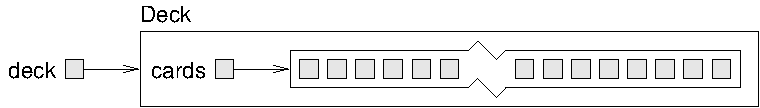
\includegraphics{figs/deckobject.pdf}
\caption{Memory diagram of an unpopulated \java{Deck} object.}
\label{fig.deckobject}
\end{center}
\end{figure}

We'll add another constructor that creates a standard 52-card array and populates it with \java{Card} objects:

\begin{code}
public Deck() {
    this.cards = new Card[52];
    int index = 0;
    for (int suit = 0; suit <= 3; suit++) {
        for (int rank = 1; rank <= 13; rank++) {
            this.cards[index] = new Card(rank, suit);
            index++;
        }
    }
}
\end{code}

This method is similar to the example in Section~\ref{cardarray}; we just turned it into a constructor.
We can now create a standard \java{Deck} like this:

\begin{code}
Deck deck = new Deck();
\end{code}

\index{printDeck}

Now that we have a \java{Deck} class, we have a logical place to put methods that pertain to decks.
Looking at the methods we have written so far, one obvious candidate is \java{printDeck} from Section~\ref{cardarray}.
%Here's how it looks, rewritten as an instance method of \java{Deck}:

\begin{code}
public void print() {
    for (Card card : this.cards) {
        System.out.println(card);
    }
}
\end{code}

%\begin{code}
%public void print() {
%    for (int i = 0; i < this.cards.length; i++) {
%        System.out.println(this.cards[i]);
%    }
%}
%\end{code}

Notice that when we transform a static method into an instance method, the code is shorter.
We can simply type \java{deck.print()} to invoke this method.


\section{Shuffling decks}
\label{shuffle}

\index{shuffle}

For most card games, you need to be able to shuffle the deck; that is, put the cards in a random order.
In Section~\ref{random} we saw how to generate random numbers, but it is not obvious how to use them to shuffle a deck.

One possibility is to model the way humans shuffle, which is usually dividing the deck in two halves and then choosing alternately from each one.
Since humans usually don't shuffle perfectly, after about seven iterations the order of the deck is pretty well randomized.

But a computer program would have the annoying property of doing a perfect shuffle every time, which is not very random.
In fact, after eight perfect shuffles, you would find the deck back in the order you started in!
For more on this, see \url{https://en.wikipedia.org/wiki/Faro_shuffle}.

\index{pseudocode}

A better shuffling algorithm is to traverse the deck one card at a time, and at each iteration, choose two cards and swap them.
To sketch an outline of how this algorithm works, we will use a combination of Java statements and English comments.
This technique is sometimes called {\bf pseudocode}.

\index{shuffle}

\begin{code}
public void shuffle() {
    for each index i {
        // choose a random number between i and length - 1
        // swap the ith card and the randomly-chosen card
    }
}
\end{code}

\index{helper method}
\index{method!helper}

The nice thing about pseudocode is that it often makes clear what other methods you are going to need.
In this case, we need a method that chooses a random integer between \java{low} and \java{high}, and a method that takes two indexes and swaps the cards at those positions.

\begin{code}
private static int randomInt(int low, int high) {
    // return a random number between low and high
}

private void swapCards(int i, int j) {
    // swap the ith and the jth cards in the array
}
\end{code}

\index{randomInt}
\index{swapCards}

Methods like \java{randomInt} and \java{swapCards} are called {\bf helper methods}, because they help you solve parts of the problem.
Helper methods are often \java{private}, since they are specific to the internal algorithms of the class.

\index{top-down design}
\index{design process}

This process of writing pseudocode first and then writing helper methods to make it work is called {\bf top-down design} (see \url{https://en.wikipedia.org/wiki/Top-down_and_bottom-up_design}).
It is similar to ``incremental development'' and ``encapsulation and generalization'', the other design processes you have seen in this book.

One of the exercises at the end of the chapter asks you to write the helper methods \java{randomInt} and \java{swapCards}, and use them to implement \java{shuffle}.


\section{Selection sort}
\label{sorting}

\index{selection sort}
\index{sort!selection}

Now that we have shuffled the deck, we need a way to put it back in order.
There is an algorithm for sorting that is ironically similar to the algorithm for shuffling.
It's called {\bf selection sort}, because it works by traversing the array repeatedly and selecting the lowest (or highest) remaining card each time.

During the first iteration, we find the lowest card and swap it with the card in the 0th position.
During the $i$th iteration, we find the lowest card to the right of $i$ and swap it with the $i$th card.
%Here is pseudocode for selection sort:

\begin{code}
public void selectionSort() {
    for each index i {
        // find the lowest card at or to the right of i
        // swap the ith card and the lowest card found
    }
}
\end{code}

Again, the pseudocode helps with the design of the helper methods.
For this algorithm we can use \java{swapCards} from before, so we only need a method to find the lowest card; we'll call it \java{indexLowest}.

\begin{code}
private int indexLowest(int low, int high) {
    // find the lowest card between low and high
}
\end{code}


One of the exercises at the end of the chapter asks you to write \java{indexLowest}, and then use it and \java{swapCards} to implement \java{selectionSort}.


\section{Merge sort}
\label{mergesort}

\index{efficiency}

Selection sort is a simple algorithm, but it is not very efficient.
To sort $n$ items, it has to traverse the array $n-1$ times.
Each traversal takes an amount of time proportional to $n$.
The total time, therefore, is proportional to $n^2$.

\index{merge sort}
\index{sort!merge}

We will develop a more efficient algorithm called {\bf merge sort}.
To sort $n$ items, merge sort takes time proportional to $n \log_2 n$.
That may not seem impressive, but as $n$ gets big, the difference between $n^2$ and $n \log_2 n$ can be enormous.

For example, $\log_2$ of one million is around 20.
So if you had to sort a million numbers, merge sort would require 20 million steps.
But selection sort would require one trillion steps!

The idea behind merge sort is this: if you have two subdecks, each of which has already been sorted, you can quickly merge them into a single, sorted deck.
Try this out with a deck of cards:

\begin{enumerate}

\item Form two subdecks with about 10 cards each, and sort them so that when they are face up the lowest cards are on top.
Place both decks face up in front of you.

\item Compare the top card from each deck and choose the lower one.
Flip it over and add it to the merged deck.

\item Repeat step 2 until one of the decks is empty.
Then take the remaining cards and add them to the merged deck.

\end{enumerate}

The result should be a single sorted deck.
In the next few sections, we'll explain how to implement this algorithm in Java.


\section{Subdecks}

\index{subdeck}

The first step of merge sort is to split the deck into two subdecks, each with about half of the cards.
So we need to write a method, \java{subdeck}, that takes a deck and a range of indexes.
It returns a new deck that contains the specified subset of the cards.

\begin{code}
public Deck subdeck(int low, int high) {
    Deck sub = new Deck(high - low + 1);
    for (int i = 0; i < sub.cards.length; i++) {
        sub.cards[i] = this.cards[low + i];
    }
    return sub;
}
\end{code}

The first line creates an unpopulated subdeck (an array of \java{null} references).
Inside the \java{for} loop, the subdeck gets populated with references in the deck.

\index{off-by-one}

The length of the subdeck is \java{high - low + 1}, because both the low card and the high card are included.
This sort of computation can be confusing, and forgetting the ``\java{+ 1}'' often leads to {\bf off-by-one} errors.
Drawing a picture is usually the best way to avoid them.

%For example, to select the middle three of five values in an array, we need \java{3 - 1 + 1} values.
%
%\begin{center}
%\begin{tabular}{ccccc}
%\hline
%\multicolumn{1}{|c|}{} & \multicolumn{1}{c|}{X} & \multicolumn{1}{c|}{X} & \multicolumn{1}{c|}{X} & \multicolumn{1}{c|}{} \\
%\hline
%0                      & 1                      & 2                      & 3                      & 4                     \\
%\end{tabular}
%\end{center}

\index{constructor}
\index{overload}

Figure~\ref{fig.subdeck} is a memory diagram of a subdeck with \java{low = 0} and \java{high = 4}.
The result is a hand with five cards that are {\em shared} with the original deck; that is, they are aliased.

\begin{figure}[!ht]
\begin{center}
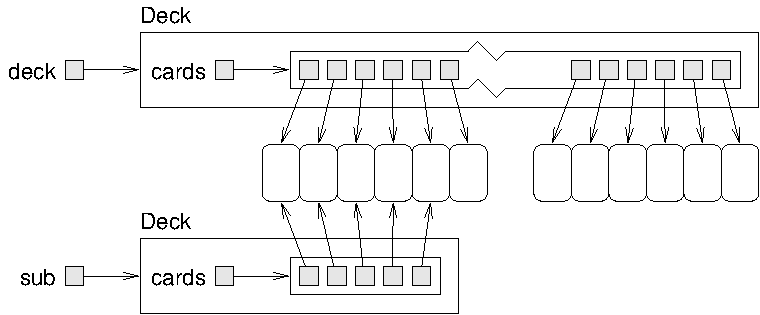
\includegraphics{figs/subdeck.pdf}
\caption{Memory diagram showing the effect of \java{subdeck}.}
\label{fig.subdeck}
\end{center}
\end{figure}

\index{aliasing}
\index{reference}

Aliasing might not be a good idea, because changes to shared cards would be reflected in multiple decks.
But since \java{Card} objects are immutable, this kind of aliasing is not a problem at all.
It also saves a lot of memory, because we never have to create duplicate \java{Card} objects.


\section{Merging decks}

\index{merge}

The next helper method we need is \java{merge}, which takes two sorted subdecks and returns a new deck containing all cards from both decks, in order.
Here's what the algorithm looks like in pseudocode, assuming the subdecks are named \java{d1} and \java{d2}:

\begin{code}
private static Deck merge(Deck d1, Deck d2) {
    // create a new deck big enough for all the cards

    // use the index i to keep track of where we are at in
    // the first deck, and the index j for the second deck
    int i = 0;
    int j = 0;

    // the index k traverses the result deck
    for (int k = 0; k < d3.length; k++) {

        // if d1 is empty, use top card from d2
        // if d2 is empty, use top card from d1
        // otherwise, compare the top two cards

        // add lowest card to the new deck at k
        // increment i or j (depending on card)
    }
    // return the new deck
}
\end{code}

An exercise at the end of the chapter asks you to implement \java{merge}.
It's somewhat tricky, so be sure to test it with different subdecks.
Once your \java{merge} method is working correctly, you can use it to write a simplified version of merge sort:

\begin{code}
public Deck almostMergeSort() {
    // divide the deck into two subdecks
    // sort the subdecks using selectionSort
    // merge the subdecks, return the result
}
\end{code}


\section{Adding recursion}

Now that we have a way to \java{merge} two decks, the real fun begins!
The magical thing about merge sort is that it is inherently recursive.
Take another look at the pseudocode for \java{almostMergeSort} in the previous section.

At the point where you sort the subdecks, why should you invoke the slower method, \java{selectionSort}?
Why not invoke the spiffy new \java{mergeSort} method, the one you are in the process of writing?
Not only is that a good idea, it is {\em necessary} to achieve the $\log_2$ performance advantage.
\index{recursion}

To make \java{mergeSort} work recursively, you have to add a base case; otherwise it repeats forever.
A simple base case is a subdeck with 0 or 1 cards.
If \java{mergeSort} receives such a small subdeck, it can return it unmodified since it would already be sorted.

The recursive version of \java{mergeSort} looks something like this:

\begin{code}
public Deck mergeSort() {
    // if the deck has 0 or 1 cards, return it
    // divide the deck into two subdecks
    // sort the subdecks using mergeSort
    // merge the subdecks, return the result
}
\end{code}

\index{leap of faith}

As usual, there are two ways to think about recursive programs: you can think through the entire flow of execution, or you can make the ``leap of faith'' (see Section~\ref{leap_of_faith}).
This example should encourage you to make the leap of faith.

When you used \java{selectionSort} to sort the subdecks, you didn't feel compelled to follow the flow of execution.
You just assumed it works because you had already debugged it.
And all you did to make \java{mergeSort} recursive was replace one sorting algorithm with another.
There is no reason to read the program any differently.

Well, almost.
You might have to give some thought to getting the base case right and making sure that you reach it eventually.
But other than that, writing the recursive version should be no problem.
The most difficult part of merge sort is the \java{merge} method, and that part is not recursive.


\section{Static context}

Figure~\ref{fig.deck} lists the \java{Deck} methods we have so far.
In UML diagrams, \java{private} methods begin with a minus sign (\java{-}), and \java{static} methods are underlined.

\index{UML}
\index{class diagram}
\index{diagram!class}

\begin{figure}[!ht]
\begin{center}
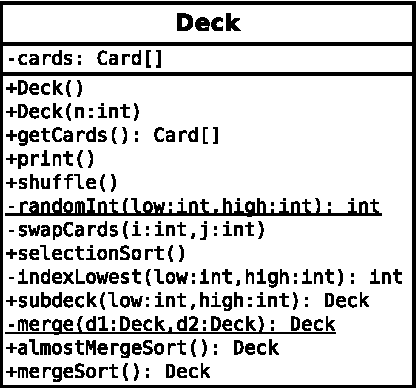
\includegraphics{figs/deck.pdf}
\caption{UML diagram for the \java{Deck} class.}
\label{fig.deck}
\end{center}
\end{figure}

The helper methods \java{randomInt} and \java{merge} are \java{static}, because they do not require \java{this.cards}.
All other methods are instance methods, because they require an instance of \java{this.cards}.
For example, you cannot invoke the \java{print} method this way:

\begin{code}
Deck.print();  // wrong!
\end{code}

% DW suggested that at some point we should warn students
% about using \java{this} in a static method

\index{static context}
\index{this}

If you try to compile this code, you will get the error, ``non-static method print() cannot be referenced from a static context.''
By {\bf static context}, the compiler means you are trying to invoke a method without passing \java{this}.
To invoke an instance method, you need an instance:

\begin{code}
Deck deck = new Deck();
deck.print();  // correct
\end{code}

Notice that \java{Deck} with a capital \java{D} is a class, and \java{deck} with a lowercase \java{d} is a variable.
When you invoke \java{deck.print()}, the reference of \java{deck} becomes the reference \java{this}.
For static methods, there is no such thing as \java{this}.

\begin{code}
private static Deck merge(Deck d1, Deck d2) {
    return this.cards;  // wrong!
}
\end{code}

If you refer to \java{this} in a static method, you will get the compiler error, ``non-static variable this cannot be referenced from a static context.''
The \java{merge} method needs to create and return a new \java{Deck} object.

%\index{sort!Arrays}
%\index{array!sorting}

%Normally we wouldn't implement two different sorting algorithms in the same class.
%Our goal with \java{Deck} was to demonstrate static methods and different ways of solving the same problem.
%In practice, we could just write a single \java{sort} method that uses \java{java.util.Arrays}.
%
%\begin{code}
%public void sort() {
%    Arrays.sort(this.cards);
%}
%\end{code}


\section{Piles of cards}

\index{War (card game)}

Now that we have classes that represent cards and decks, let's use them to make a game.
One of the simplest card games that children play is called ``War'' (see \url{https://en.wikipedia.org/wiki/War_(card_game)}).

In this game, the deck is divided into two or more piles.
Players take turns revealing the top card of their pile.
Whoever has the highest ranking card takes the two cards.
If there is a tie, players draw four more cards.
Whoever has the highest ranking fourth card takes all ten cards.
The game continues until one player has won the entire deck.

We could use the \java{Deck} class to represent the individual piles.
However, our implementation of \java{Deck} uses a \java{Card} array, and the length of an array can't change.
As the game progresses, we need to be able to add and remove cards from the piles.

\index{ArrayList}
\index{collection}

We can solve this problem by using an \java{ArrayList}, which is in the \java{java.util} package.
An \java{ArrayList} is a {\bf collection}, which is an object that contains other objects.
It provides methods to add and remove elements, and it grows and shrinks automatically.

%The Java library includes many other collections (see \url{https://docs.oracle.com/javase/8/docs/technotes/guides/collections/}).
%For our purposes, \java{ArrayList} is a good choice because it provides methods to add and remove elements, and it grows and shrinks automatically.

\index{Pile}
\index{class!Pile}

We will define a new class named \java{Pile} that represents a pile of cards.
It uses an \java{ArrayList} (instead of an array) to store the \java{Card} objects.

\begin{code}
public class Pile {
    private ArrayList<Card> cards;

    public Pile() {
        this.cards = new ArrayList<Card>();
    }
}
\end{code}

\index{angle brackets}
\index{brackets!angle}
\index{\textless\textgreater\ angle brackets}

When you declare an \java{ArrayList}, you specify the type it contains in angle brackets (\java{<>}).
This declaration says that \java{cards} is not just an \java{ArrayList}, it's an \java{ArrayList} of \java{Card} objects.
The constructor initializes \java{this.cards} with an empty \java{ArrayList}.

%Java collections can only store objects, not primitives like \java{int}.
%But you can use wrapper classes, for example \java{ArrayList<Integer>}.

\java{ArrayList} provides a method, \java{add}, that adds an element to the collection.
We will write a \java{Pile} method that does the same thing:

\begin{code}
public void addCard(Card card) {
    this.cards.add(card);        // to the bottom of the pile
}
\end{code}

\index{this}

We also need to be able to remove cards from the top (or front) of the pile.
If we use \java{ArrayList.remove}, it will automatically shift the remaining cards left to fill the gap.

\begin{code}
public Card popCard() {
    return this.cards.remove(0);  // from the top of the pile
}
\end{code}

In order to know when to stop the game, we need to know how many cards are in each pile.

\begin{code}
public int size() {
    return this.cards.size();
}
\end{code}

\index{wrapper method}

Methods like \java{addCard}, \java{popCard}, and \java{size}, which invoke another method without doing much additional work, are called {\bf wrapper methods}.
The last method we need adds an entire subdeck to the pile.

\begin{code}
public void addDeck(Deck deck) {
    for (Card card : deck.getCards()) {
        this.cards.add(card);
    }
}
\end{code}

Now we can use \java{Deck} and \java{Pile} to implement the game.
The \java{main} method begins like this:

\begin{code}
// create and shuffle the deck
Deck deck = new Deck();
deck.shuffle();

// divide the deck into piles
Pile p1 = new Pile();
p1.addDeck(deck.subdeck(0, 25));
Pile p2 = new Pile();
p2.addDeck(deck.subdeck(26, 51));
\end{code}

The game itself is a loop that repeats until one of the piles is empty.
At each iteration, we draw a card from each pile and compare their ranks.

\begin{code}
// while both piles are not empty
while (p1.size() > 0 && p2.size() > 0) {
    Card c1 = p1.popCard();
    Card c2 = p2.popCard();

    // compare the cards
    int diff = c1.getRank() - c2.getRank();
    if (diff > 0) {
        p1.addCard(c1);
        p1.addCard(c2);
    } else if (diff < 0) {
        p2.addCard(c1);
        p2.addCard(c2);
    } else {  // it's a tie...draw four more cards
\end{code}

One of the exercises at the end of this chapter asks you to implement the \java{else} block when there's a tie.
After the \java{while} loop ends, we display the winner based on which pile is not empty.

\begin{code}
if (p1.size() > 0) {
    System.out.println("Player 1 wins!");
} else {
    System.out.println("Player 2 wins!");
}
\end{code}

\java{ArrayList} provides many other methods that we didn't use for this example program.
Take a minute to read about them in the Java documentation.


\section{Vocabulary}

\begin{description}

\term{pseudocode}
A way of designing programs by writing rough drafts in a combination of English and Java.

\term{helper method}
Often a small method that does not do anything enormously useful by itself, but which helps another, more complex method.

\term{top-down design}
Breaking down a problem into sub-problems, and solving each sub-problem one at a time.

\term{selection sort}
A simple sorting algorithm that searches for the smallest or largest element $n$ times.

\term{merge sort}
A recursive sorting algorithm that divides an array into two parts, sorts each part (using merge sort), and merges the results.

\term{off-by-one}
A common programming mistake that results in iterating one too few times (or one too many).

\term{static context}
The parts of a class that run without reference to a specific instance of the class.

\term{collection}
A Java library class (such as \java{ArrayList}) that represents a group of objects.

\term{wrapper method}
A method that calls another method without doing much additional work.

%\term{insertion sort}
%Another sorting algorithm that inserts elements into place, one at a time.

\end{description}


\section{Exercises}

The code for this chapter is in the {\tt ch13} directory of {\tt ThinkJavaCode2}.
See page~\pageref{code} for instructions on how to download the repository.
Before you start the exercises, we recommend that you compile and run the examples.


\begin{exercise}  %%V6 Ex13.5

Write a \java{toString} method for the \java{Deck} class.
It should return a single string that represents the cards in the deck.
When it's printed, this string should display the same results as the \java{print} method in Section~\ref{deck}.

\index{StringBuilder}
\index{efficiency}

{\it Hint:} You can use the \java{+} operator to concatenate strings, but it is not very efficient.
Consider using \java{java.lang.StringBuilder} instead; you can review the documentation by doing a web search for ``Java StringBuilder''.

\end{exercise}


\begin{exercise}  %%V6 Ex13.2
\label{ex.shuffle}

The goal of this exercise is to implement the shuffling algorithm from this chapter.

\begin{enumerate}

\item In the repository for this book, you should find the file named {\tt Deck.java}.
Check that you can compile it in your environment.

\item Implement the \java{randomInt} method.
You can use the \java{nextInt} method provided by \java{java.util.Random}, which we saw in Section~\ref{random}.

{\it Hint:} Avoid creating a \java{Random} object every time \java{randomInt} is invoked by defining a class variable.

\item Implement the \java{swapCards} method that takes two indexes and swaps the cards at the given locations.

\item Implement the \java{shuffle} method using the algorithm in Section~\ref{shuffle}.

\end{enumerate}

\end{exercise}


\begin{exercise}  %%V6 Ex13.3

The goal of this exercise is to implement the sorting algorithms from this chapter.
Use the {\tt Deck.java} file from the previous exercise, or create a new one from scratch.

\begin{enumerate}

\item Implement the \java{indexLowest} method.
Use the \java{Card.compareTo} method to find the lowest card in a given range of the deck (from \java{lowIndex} to \java{highIndex}, including both).

\item Implement \java{selectionSort} using the algorithm in Section~\ref{sorting}.

\item Using the pseudocode in Section~\ref{mergesort}, implement the \java{merge} method.
The best way to test it is to build and shuffle a deck.
Then use \java{subdeck} to form two small subdecks, and use selection sort to sort them.
Finally, pass the two halves to \java{merge} and see if it works.
\index{testing}

\item Implement \java{almostMergeSort}, the one that divides the deck in half, uses \java{selectionSort} to sort the two halves, and uses \java{merge} to create a new, sorted deck.
You should be able to reuse code from the previous step.

\item Implement \java{mergeSort} recursively.
Remember that \java{selectionSort} is a modifier and \java{mergeSort} is a pure method, which means that they get invoked differently:

\begin{code}
deck.selectionSort();      // modifies an existing deck
deck = deck.mergeSort();   // replaces old deck with new
\end{code}

\end{enumerate}

\end{exercise}


\begin{exercise}

%%V6 Ex13.1
You can learn more about the sorting algorithms in this chapter, and others, at \href{http://www.sorting-algorithms.com/}{sorting-algorithms.com}.
This site provides explanations of the algorithms and animations that show how they work.
It also includes an analysis of their efficiency.

%%V6 Ex13.4
For example, ``insertion sort'' is an algorithm that inserts elements into place, one at a time.
Read about it at \url{http://www.sorting-algorithms.com/insertion-sort}.
Then write a method named \java{insertionSort} that implements this algorithm.

One goal of this exercise is to practice top-down design.
Your solution should use a helper method, named \java{insert}, that implements the inner loop of the algorithm.
\java{insertionSort} should invoke this method $n-1$ times.


\end{exercise}


\begin{exercise}  %%V6.5 NEW

Find and open the file \java{War.java} in the repository.
The \java{main} method contains all the code from the last section of this chapter.
Check that you can compile and run this code before proceeding.

The program is incomplete; it does not handle the case when two cards have the same rank.
Finish implementing the \java{main} method beginning at the line that says: \java{// it's a tie...draw four more cards}.

When there's a tie, draw three cards from each pile and store them in a collection, along with the original two.
Then draw one more card from each pile and compare them.
Whoever wins the tie will take all ten of these cards.

If one pile does not have at least four cards, the game ends immediately.
If a tie ends with a tie, flip a coin and give the cards to one of the players.

Notice that this program depends on \java{Deck.shuffle}.
If you haven't implemented the \java{shuffle} method (see Exercise~\ref{ex.shuffle}), the game won't be that fun.
Player 1 will have the Ace through King of the first two suits, and Player 2 will have the the Ace through King of the other two suits, all in the same order.

\end{exercise}


\begin{exercise}  %%V6.5 NEW

Extend your program from the previous exercise to handle the case when a tie ends with a tie.
In other words, when the fourth cards have the same rank, add three more cards to the collection and try again.
You will need to wrap your code in a loop, for example: \java{while (diff == 0)}.

\end{exercise}


\chapter{Extending classes}
\label{eights}

\index{Crazy Eights}

In this chapter, we will present a comprehensive example of object-oriented programming.
{\it Crazy Eights} is a classic card game for two or more players.
The main objective is to be the first player to get rid of all your cards.
Here's how to play:

\begin{itemize}

\item Deal five or more cards to each player, and then deal one card face up to create the ``discard pile''.
Place the remaining cards face down to create the ``draw pile''.

\item Each player takes turns placing a single card on the discard pile.
The card must match the rank or suit of the previously played card, or be an eight, which is a ``wild card''.

\item When players don't have a matching card or an eight, they must draw new cards until they get one.

\item If the draw pile ever runs out, the discard pile is shuffled (except the top card) and becomes the new draw pile.

\item As soon as a player has no cards, the game ends and all other players score penalty points for their remaining cards.
Eights are worth 20, face cards are worth 10, and all others are worth their rank.

\end{itemize}

You can read \url{https://en.wikipedia.org/wiki/Crazy_Eights} for more details, but we have enough to get started.

%The code for this chapter is in the directory {\tt ch14} in the repository for this book.
%Instructions for downloading this code are on page~\pageref{code}.


\section{CardCollection}

To implement {\it Crazy Eights}, we need to represent a deck of cards, a discard pile, a draw pile, and a hand for each player.
And we need to be able to deal, draw, and discard cards.

The \java{Deck} and \java{Pile} classes from the previous chapter meet some of these requirements.
But unless we make some changes, neither of them can be used to represent a hand of cards that well.

\index{ArrayList}

Furthermore, \java{Deck} and \java{Pile} are essentially two versions of the same code: one based on arrays, and the other based on \java{ArrayList}.
It would be helpful to combine their features into one class that meets the needs of both.
%We could potentially use such a class for other collections of cards.

We will define a class named \java{CardCollection} and add the code we want one step at a time.
Since this class will represent different piles and hands of cards, we'll add a \java{label} attribute to tell them apart.

\index{CardCollection}
\index{class!CardCollection}

\begin{code}
public class CardCollection {

    private String label;
    private ArrayList<Card> cards;

    public CardCollection(String label) {
        this.label = label;
        this.cards = new ArrayList<Card>();
    }
}
\end{code}

%Both instance variables are \java{private}, so we will not be able to access them from other classes (including subclasses).
%That will turn out to be too restrictive; in the next section we will have to change it.

As with the \java{Pile} class, we need a way to add cards to the collection.
Here is the \java{addCard} method from the previous chapter:

\begin{code}
public void addCard(Card card) {
    this.cards.add(card);
}
\end{code}

\index{this}

Until now, we have used \java{this} explicitly to make it easy to identify attributes.
Inside \java{addCard} and other instance methods, you can access instance variables without using the keyword \java{this}.
So from here on, we will drop it:

\begin{code}
public void addCard(Card card) {
    cards.add(card);
}
\end{code}

We also need to be able to remove cards from the collection.
The following method takes an index, removes the card at that location, and shifts the following cards left to fill the gap:

\begin{code}
public Card popCard(int i) {
    return cards.remove(i);
}
\end{code}

\index{efficiency}

If we are dealing cards from a shuffled deck, we don't care which card gets removed.
It is most efficient to choose the last one, so we don't have to shift any cards left.
Here is an overloaded version of \java{popCard} that removes and returns the last card:

\begin{code}
public Card popCard() {
    int i = size() - 1;     // from the end of the collection
    return popCard(i);
}
\end{code}

Notice that \java{popCard} uses \java{CardCollection}'s own \java{size} method, which in turn calls the \java{ArrayList}'s \java{size} method:

\begin{code}
public int size() {
    return cards.size();
}
\end{code}

For convenience, \java{CardCollection} also provides an \java{empty} method that returns \java{true} when \java{size} is zero:

\begin{code}
public boolean empty() {
    return cards.size() == 0;
}
\end{code}

To access the elements of an \java{ArrayList}, you can't use the array \java{[]} operator.
Instead, you have to use the methods \java{get} and \java{set}.
Here is a wrapper for \java{get}:

\begin{code}
public Card getCard(int i) {
    return cards.get(i);
}
\end{code}

The \java{lastCard} method gets the last card (but doesn't remove it):

\begin{code}
public Card lastCard() {
    int i = size() - 1;
    return cards.get(i);
}
\end{code}

\index{modifier method}
\index{method!modifier}

In order to control the ways card collections are modified, we don't provide a wrapper for \java{set}.
The only modifiers we provide are the two versions of \java{popCard} and the following version of \java{swapCards}:

\begin{code}
public void swapCards(int i, int j) {
    Card temp = cards.get(i);
    cards.set(i, cards.get(j));
    cards.set(j, temp);
}
\end{code}

We use \java{swapCards} to implement \java{shuffle}, which we described in Section~\ref{shuffle}:

\begin{code}
public void shuffle() {
    Random random = new Random();
    for (int i = size() - 1; i > 0; i--) {
        int j = random.nextInt(i);
        swapCards(i, j);
    }
}
\end{code}


\section{Inheritance}

At this point we have a class that represents a collection of cards.
It provides functionality common to decks of cards, piles of cards, hands of cards, and potentially other collections.

\index{inheritance}
\index{subclass}
\index{extends}

However, each kind of collection will be slightly different.
Rather than add every possible feature to \java{CardCollection}, we can use {\bf inheritance} to define subclasses.
A {\bf subclass} is a class that ``extends'' an existing class; that is, it has the attributes and methods of the existing class, plus more.

Here is the complete definition of our new and improved \java{Deck} class:

\begin{code}
public class Deck extends CardCollection {

    public Deck(String label) {
        super(label);
        for (int suit = 0; suit <= 3; suit++) {
            for (int rank = 1; rank <= 13; rank++) {
                cards.add(new Card(rank, suit));
            }
        }
    }
}
\end{code}

\index{extends}
\index{superclass}

The first line uses the keyword \java{extends} to indicate that \java{Deck} extends the class \java{CardCollection}.
That means a \java{Deck} object has the same instance variables and methods as a \java{CardCollection}.
Another way to say the same thing is that \java{Deck} ``inherits from'' \java{CardCollection}.
We could also say that \java{CardCollection} is a {\bf superclass}, and \java{Deck} is one of its subclasses.

% NOTE: Let's stick with ``superclass'' and ``subclass'' and
% not use ``parent'' and ``child''.

\index{Object class}

In Java, classes may only extend one superclass.
Classes that do not specify a superclass with \java{extends} automatically inherit from \java{java.lang.Object}.
So in this example, \java{Deck} extends \java{CardCollection}, which in turn extends \java{Object}.
The \java{Object} class provides the default \java{equals} and \java{toString} methods, among other things.

Constructors are not inherited, but all other \java{public} attributes and methods are.
The only additional method in \java{Deck}, at least for now, is a constructor.
So you can create a \java{Deck} object like this:

\begin{code}
Deck deck = new Deck("Deck");
\end{code}

The first line of the constructor uses \java{super}, which is a keyword that refers to the superclass of the current class.
When \java{super} is used like a method, as in this example, it invokes the constructor of the superclass.

%TODO: Blythe suggests a diagram here

So in this case, \java{super} invokes the \java{CardCollection} constructor, which initializes the attributes \java{label} and \java{cards}.
When it returns, the \java{Deck} constructor resumes and populates the (empty) \java{ArrayList} with \java{Card} objects.

That's it for the \java{Deck} class.
Next we need a way to represent a hand, which is the collection of cards held by a player, and a pile, which is a collection of cards on the table.
We could define two classes, one for hands and one for piles, but there is not much difference between them.
So we'll use one class, called \java{Hand}, for both hands and piles.
Here's what the definition looks like:

\index{Hand}
\index{class!Hand}

\begin{code}
public class Hand extends CardCollection {

    public Hand(String label) {
        super(label);
    }

    public void display() {
        System.out.println(getLabel() + ": ");
        for (int i = 0; i < size(); i++) {
            System.out.println(getCard(i));
        }
        System.out.println();
    }
}
\end{code}

Like \java{Deck}, the \java{Hand} class extends \java{CardCollection}.
So it inherits methods like \java{getLabel}, \java{size}, and \java{getCard}, which are used in \java{display}.
\java{Hand} also provides a constructor, which invokes the constructor of \java{CardCollection}.
%But in this case the only thing the new constructor does is invoke the constructor from the superclass, using \java{super}.

In summary, a \java{Deck} is just like a \java{CardCollection}, but it provides a different constructor.
And a \java{Hand} is just like a \java{CardCollection}, but it provides an additional method, \java{display}.


\section{Dealing cards}
\label{dealing}

To begin the game, we need to deal cards to each of the players.
And during the game, we need to move cards between hands and piles.
If we add the following method to \java{CardCollection}, it can meet both of these requirements.

\begin{code}
public void deal(CardCollection that, int n) {
    for (int i = 0; i < n; i++) {
        Card card = popCard();
        that.addCard(card);
    }
}
\end{code}

The \java{deal} method removes cards from the collection it is invoked on, \java{this}, and adds them to the collection it gets as a parameter, \java{that}.
The second parameter, \java{n}, is the number of cards to deal.
We will use this method to implement \java{dealAll}, which deals (or moves) all of the remaining cards.

\begin{code}
public void dealAll(CardCollection that) {
    int n = size();
    deal(that, n);
}
\end{code}

At this point we can create a \java{Deck} and start dealing cards.
Here's a simple example that deals five cards to a hand, and deals the rest into a draw pile:

\begin{code}
Deck deck = new Deck("Deck");
deck.shuffle();

Hand hand = new Hand("Hand");
deck.deal(hand, 5);
hand.display();

Hand drawPile = new Hand("Draw Pile");
deck.dealAll(drawPile);
System.out.printf("Draw Pile has %d cards.\n",
                  drawPile.size());
\end{code}

Because the deck is shuffled randomly, you should get a different hand each time you run this example.
The output will look something like:

\begin{stdout}
Hand:
5 of Diamonds
Ace of Hearts
6 of Clubs
6 of Diamonds
2 of Clubs

Draw Pile has 47 cards.
\end{stdout}

If you are a careful reader, you might notice something strange about this example.
Take another look at the definition of \java{deal}.
Notice that the first parameter is supposed to be a \java{CardCollection}.
But we invoked it like this:

\begin{code}
Hand hand = new Hand("Hand");
deck.deal(hand, 5);
\end{code}

The argument is a \java{Hand}, not a \java{CardCollection}.
So why is this example legal?
It's because \java{Hand} is a subclass of \java{CardCollection}, so a \java{Hand} object is also considered to be a \java{CardCollection} object.
If a method expects a \java{CardCollection}, you can give it a \java{Hand}, a \java{Deck}, or a \java{CardCollection}.

But it doesn't work the other way around: not every \java{CardCollection} is a \java{Hand}, so if a method expects a \java{Hand}, you have to give it a \java{Hand}, not a \java{CardCollection} or a \java{Deck}.

If it seems strange that an object can belong to more than one type, remember that this happens in real life, too.
Every cat is also a mammal, and every mammal is also an animal.
But not every animal is a mammal, and not every mammal is a cat.

%TODO: Blythe suggests a diagram here


\section{The Player class}

The \java{Deck} and \java{Hand} classes we have defined so far could be used for any card game; we have not yet implemented any of the rules specific to {\it Crazy Eights}.
And that's probably a good thing, since it makes it easy to reuse these classes if we want to make another game in the future.

But now it's time to implement the rules.
We'll use two classes: \java{Player}, which encapsulates player strategy, and \java{Eights}, which creates and maintains the state of the game.
Here is the beginning of the \java{Player} definition:

\index{Player}
\index{class!Player}

\begin{code}
public class Player {

    private String name;
    private Hand hand;

    public Player(String name) {
        this.name = name;
        this.hand = new Hand(name);
    }
\end{code}

A \java{Player} has two \java{private} attributes: a name and a hand.
The constructor takes the player's name as a string and saves it in an instance variable.
In this example, we have to use \java{this} to distinguish between the instance variable and the parameter with the same name.

The primary method that \java{Player} provides is \java{play}, which decides which card to discard during each turn:

\begin{code}
public Card play(Eights eights, Card prev) {
    Card card = searchForMatch(prev);
    if (card == null) {
        card = drawForMatch(eights, prev);
    }
    return card;
}
\end{code}

The first parameter is a reference to the \java{Eights} object that encapsulates the state of the game.
We'll need it if we have to draw a new card.
The second parameter, \java{prev}, is the card on top of the discard pile.

\index{top-down development}

Using top-down development, the \java{play} method invokes two helper methods, \java{searchForMatch} and \java{drawForMatch}.
The first method looks in the player's hand for a card that matches the previously played card:

\begin{code}
public Card searchForMatch(Card prev) {
    for (int i = 0; i < hand.size(); i++) {
        Card card = hand.getCard(i);
        if (cardMatches(card, prev)) {
            return hand.popCard(i);
        }
    }
    return null;
}
\end{code}

The strategy is pretty simple: the \java{for} loop searches for the first card that's legal to play and returns it.
If there are no cards that match, it returns \java{null}.
And in that case, we have to draw cards until we get a match.

\begin{code}
public Card drawForMatch(Eights eights, Card prev) {
    while (true) {
        Card card = eights.drawCard();
        System.out.println(name + " draws " + card);
        if (cardMatches(card, prev)) {
            return card;
        }
        hand.addCard(card);
    }
}
\end{code}

The \java{while} loop runs until it finds a match (we'll assume for now that it always does).
It uses the \java{Eights} object to draw a card.
If it matches, it returns the card.
Otherwise it adds the card to the player's hand and repeats.

Both \java{searchForMatch} and \java{drawForMatch} use \java{cardMatches}, which is a static method, also defined in \java{Player}.
This method is a straightforward translation of the rules of the game:

\begin{code}
public static boolean cardMatches(Card card1, Card card2) {
    if (card1.getSuit() == card2.getSuit()) {
        return true;
    }
    if (card1.getRank() == card2.getRank()) {
        return true;
    }
    if (card1.getRank() == 8) {
        return true;
    }
    return false;
}
\end{code}

Finally, \java{Player} provides a \java{score} method, which computes penalty points for cards left in a player's hand at the end of the game.

%\begin{code}
%public int score() {
%    int sum = 0;
%    for (int i = 0; i < hand.size(); i++) {
%        Card card = hand.getCard(i);
%        int rank = card.getRank();
%        if (rank == 8) {
%            sum -= 20;
%        } else if (rank > 10) {
%            sum -= 10;
%        } else {
%            sum -= rank;
%        }
%    }
%    return sum;
%}
%\end{code}


\section{The Eights class}

\index{top-down development}

In Section~\ref{shuffle} we introduced top-down development, which is a way of developing programs by identifying high-level goals, like shuffling a deck, and breaking them into smaller problems, like finding the lowest element in an array or swapping two elements.

\index{bottom-up design}
\index{design process}

In this section we present {\bf bottom-up design}, which goes the other way around: first we identify simple pieces we need, then we assemble them into more complex algorithms.

Looking at the rules of {\it Crazy Eights}, we can identify some of the methods we'll need:

\begin{itemize}

\item Create the deck, the players, and the discard and draw piles. Deal the cards and set up the game. (\java{Eights} constructor)

\item Check whether the game is over. (\java{isDone})

\item If the draw pile is empty, shuffle the discard pile and move the cards into the draw pile. (\java{reshuffle})

\item Draw a card, reshuffling the discard pile if necessary. (\java{drawCard})

\item Keep track of whose turn it is, and switch from one player to the next. (\java{nextPlayer})

\item Display the state of the game, and wait for the user before running the next turn. (\java{displayState})

\end{itemize}

Now we can start implementing the pieces.
Here is the beginning of the class definition for \java{Eights}, which encapsulates the state of the game:

\index{Eights}
\index{class!Eights}

\begin{code}
public class Eights {

    private Player one;
    private Player two;
    private Hand drawPile;
    private Hand discardPile;
    private Scanner in;
\end{code}

In this version, there are always two players.
One of the exercises at the end of the chapter asks you to modify this code to handle more players.
The \java{Eights} class also includes a draw pile, a discard pile, and a \java{Scanner}, which we will use to prompt the user after each turn.

The constructor for \java{Eights} initializes the instance variables and deals the cards, similar to Section~\ref{dealing}.
%
%\begin{code}
%public Eights() {
%    Deck deck = new Deck("Deck");
%    deck.shuffle();
%
%    int handSize = 5;
%    one = new Player("Allen");
%    deck.deal(one.getHand(), handSize);
%
%    two = new Player("Chris");
%    deck.deal(two.getHand(), handSize);
%
%    discardPile = new Hand("Discards");
%    deck.deal(discardPile, 1);
%
%    drawPile = new Hand("Draw pile");
%    deck.dealAll(drawPile);
%
%    in = new Scanner(System.in);
%}
%\end{code}
%
The next piece we'll need is a method that checks whether the game is over.
If either hand is empty, we're done:

\begin{code}
public boolean isDone() {
    return one.getHand().empty() || two.getHand().empty();
}
\end{code}

When the draw pile is empty, we have to shuffle the discard pile.
Here is a method for that:

\begin{code}
public void reshuffle() {
    Card prev = discardPile.popCard();
    discardPile.dealAll(drawPile);
    discardPile.addCard(prev);
    drawPile.shuffle();
}
\end{code}

The first line saves the top card from \java{discardPile}.
The next line transfers the rest of the cards to \java{drawPile}.
Then we put the saved card back into \java{discardPile} and shuffle \java{drawPile}.
We can use \java{reshuffle} as part of the \java{draw} method:

\begin{code}
public Card drawCard() {
    if (drawPile.empty()) {
        reshuffle();
    }
    return drawPile.popCard();
}
\end{code}

%We can switch from one player to the next like this:
The \java{nextPlayer} method takes the current player as a parameter and returns the player who should go next.

\begin{code}
public Player nextPlayer(Player current) {
    if (current == one) {
        return two;
    } else {
        return one;
    }
}
\end{code}

The last method from our bottom-up design is \java{displayState}.
It displays the hand of each player, the contents of the discard pile, and how many cards are in the draw pile.
Finally, it waits for the user to press the {\sf Enter} key.

%\begin{code}
%public void displayState() {
%    one.display();
%    two.display();
%    discardPile.display();
%    System.out.println("Draw pile:");
%    System.out.println(drawPile.size() + " cards");
%    in.nextLine();
%}
%\end{code}

Using these pieces, we can write \java{takeTurn}, which executes one player's turn.
It reads the top card off the discard pile and passes it to \java{player.play}, which we saw in the previous section.
The result is the card the player chose, which is added to the discard pile.

\begin{code}
public void takeTurn(Player player) {
    Card prev = discardPile.lastCard();
    Card next = player.play(this, prev);
    discardPile.addCard(next);

    System.out.println(player.getName() + " plays " + next);
    System.out.println();
}
\end{code}

Finally, we use \java{takeTurn} and the other methods to write \java{playGame}:

\begin{code}
public void playGame() {
    Player player = one;

    // keep playing until there's a winner
    while (!isDone()) {
        displayState();
        takeTurn(player);
        player = nextPlayer(player);
    }

    // display the final score
    one.displayScore();
    two.displayScore();
}
\end{code}

Done!
Notice the result of bottom-up design is similar to top-down: we have a high-level method that calls helper methods.
The main difference is the order we used to arrive at this solution.


\section{Class relationships}

\index{class!relationships}

This chapter demonstrates two common relationships between classes:

\begin{description}

\term{composition}
Instances of one class contain references to instances of another class.
For example, an instance of \java{Eights} contains references to two \java{Player} objects, two \java{Hand} objects, and a \java{Scanner}.

\term{inheritance}
One class extends another class.
For example, \java{Hand} extends \java{CardCollection}, so every instance of \java{Hand} is also a \java{CardCollection}.

\end{description}

\index{HAS-A}
\index{IS-A}
\index{object-oriented}

Composition is also known as a {\bf HAS-A} relationship, as in ``\java{Eights} HAS-A \java{Scanner}''.
Inheritance is also known as an {\bf IS-A} relationship, as in ``a \java{Hand} IS-A \java{CardCollection}''.
This vocabulary provides a concise way to talk about an object-oriented design.

% ABD: I would like to call these UML class diagrams to distinguish
% them from the 3172 other kinds of UML diagrams, and to be consistent
% with https://en.wikipedia.org/wiki/Class_diagram

\index{UML}
\index{class diagram}
\index{diagram!class}

There is also a standard way to represent these relationships graphically in UML class diagrams.
As we saw in Section~\ref{UML}, the UML representation of a class is a box with three sections: the class name, the attributes, and the methods.
The latter two sections are optional when showing relationships.

%NOTE: I am not using standard arrows for aggregation and composition, but
% a simplified version for all HAS-A relationships.  This is consistent
% with the class diagrams in Head First Design Patterns.

Relationships between classes are represented by arrows: composition arrows have a standard arrow head, and inheritance arrows have a hollow triangle head (usually pointing up).
Figure~\ref{fig.uml1} shows the classes defined in this chapter and the relationships among them.

%TODO: Blythe suggests picture of each arrow, but it's a pain.

\begin{figure}[!ht]
\begin{center}
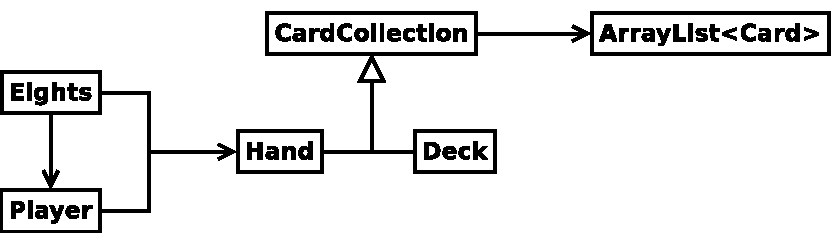
\includegraphics[width=0.8\textwidth]{figs/uml1.pdf}
\caption{UML diagram for the classes in this chapter.}
\label{fig.uml1}
\end{center}
\end{figure}

UML is an international standard, so almost any software engineer in the world could look at this diagram and understand our design.
And class diagrams are only one of many graphical representations defined in the UML standard.

We hope this final chapter has been a useful summary of all the techniques presented in the book, including variables, methods, conditionals, loops, arrays, objects, and algorithms.
Congratulations on making it to the end!


\section{Vocabulary}

\begin{description}

\term{inheritance}
The ability to define a new class that has the same instance variables and methods of an existing class.

\term{subclass}
A class that inherits from, or extends, an existing class.

\term{superclass}
An existing class that is extended by another class.

%\term{override}
%To define a method in a subclass that replaces a method with the same name in a superclass.

\term{bottom-up design}
A way of developing programs by identifying simple pieces, implementing them, and then assembling them into more complex algorithms.

\term{HAS-A}
A relationship between two classes where one class ``has'' an instance of another class as one of its attributes.

\term{IS-A}
A relationship between two classes where one class extends another class; the subclass ``is'' an instance of the superclass.

\end{description}


\section{Exercises}

The code for this chapter is in the {\tt ch14} directory of {\tt ThinkJavaCode2}.
See page~\pageref{code} for instructions on how to download the repository.
Before you start the exercises, we recommend that you compile and run the examples.


\begin{exercise}  %%V6 Ex14.1

Design a better strategy for the \java{Player.play} method.
For example, if there are multiple cards you can play, and one of them is an eight, you might want to play the eight.

\index{override}

Think of other ways you can minimize penalty points, such as playing the highest-ranking cards first.
Write a new class that extends \java{Player} and overrides \java{play} to implement your strategy.

\end{exercise}


\begin{exercise}  %%V6 Ex14.2

Write a loop that plays the game 100 times and keeps track of how many times each player wins.
If you implemented multiple strategies in the previous exercise, you can play them against each other to evaluate which one works best.

{\it Hint:} Design a \java{Genius} class that extends \java{Player} and overrides the \java{play} method, and then replace one of the players with a \java{Genius} object.

\end{exercise}


\begin{exercise}  %%V6 Ex14.3

One limitation of the program we wrote in this chapter is that it only handles two players.
Modify the \java{Eights} class to create an \java{ArrayList} of players, and modify \java{nextPlayer} to select the next player.

\end{exercise}


\begin{exercise}  %%V6 Ex14.4

When we designed the program for this chapter, we tried to minimize the number of classes.
As a result, we ended up with a few awkward methods.
For example, \java{cardMatches} is a static method in \java{Player}, but it would be more natural if it were an instance method in \java{Card}.

The problem is that \java{Card} is supposed to be useful for any card game, not just {\it Crazy Eights}.
You can solve this problem by adding a new class, \java{EightsCard}, that extends \java{Card} and provides a method, \java{match}, that checks whether two cards match according to the rules of {\it Crazy Eights}.

At the same time, you could create a new class, \java{EightsHand}, that extends \java{Hand} and provides a method, \java{scoreHand}, that adds up the scores of the cards in the hand.
And while you're at it, you could add a method named \java{scoreCard} to \java{EightsCard}.

Whether or not you actually make these changes, draw a UML class diagram that shows this alternative object hierarchy.

\end{exercise}


\appendix
\addtocontents{toc}{\protect\newpage}

%BEGIN LATEX
\renewcommand{\chaptermark}[1]{\markboth{Appendix \thechapter ~~ #1}{}}
%END LATEX

\chapter{Tools}
\label{tools}

\index{IDE}

The steps for compiling, running, and debugging Java code depend on your development environment and operating system.
We avoided putting these details in the main text, because they can be distracting.
Instead, we provide this appendix with a brief introduction to DrJava -- an {\bf integrated development environment} (IDE) that is helpful for beginners -- and other development tools, including Checkstyle for code quality and JUnit for testing.


\section{Installing DrJava}
\label{drjava}

The easiest way to start programming in Java is to use a website that compiles and runs Java code in the browser.
Examples include \href{https://trinket.io/}{\tt trinket.io}, \href{https://repl.it/}{\tt repl.it}, \href{https://www.jdoodle.com/}{\tt jdoodle.com}, and others.

If you are unable to install software on your computer (which is often the case in public schools and Internet caf\'{e}s), you can use these online development environments for almost everything in this book.

But if you want to compile and run Java programs on your own computer, you will need:

\begin{itemize}

\item The {\bf Java Development Kit} (JDK), which includes the compiler, the {\bf Java Virtual Machine} (JVM) that interprets the compiled byte code, and other tools such as Javadoc.

\index{JDK}
\index{JVM}
\index{virtual machine}
\index{Javadoc}

\index{text editor}
\index{DrJava}

\item A {\bf text editor} such as Atom, Notepad++, or Sublime Text, and/or an IDE such as DrJava, Eclipse, jGrasp, or NetBeans.

\end{itemize}

The JDK we recommend is Java SE (Standard Edition), which Oracle makes available for free.
The IDE we recommend is DrJava, which is an open-source development environment written in Java (see Figure~\ref{fig.drjava1}).

To install the JDK, search the web for ``download JDK'' which should take you to Oracle's website.
Scroll down to ``Java Platform, Standard Edition'' and click the download button under JDK.
Then accept the license agreement and select the installer for your operating system.
Don't forget to run the installer after you download it!

\index{JAR}

To install DrJava, visit \url{http://drjava.org/} and download the {\bf JAR} file.
We recommend that you save it to your Desktop or another convenient location.
Simply double-click the JAR file to run DrJava.
Refer to the DrJava documentation (\url{http://drjava.org/docs/quickstart/}) for more details.

\begin{figure}[!ht]
\begin{center}
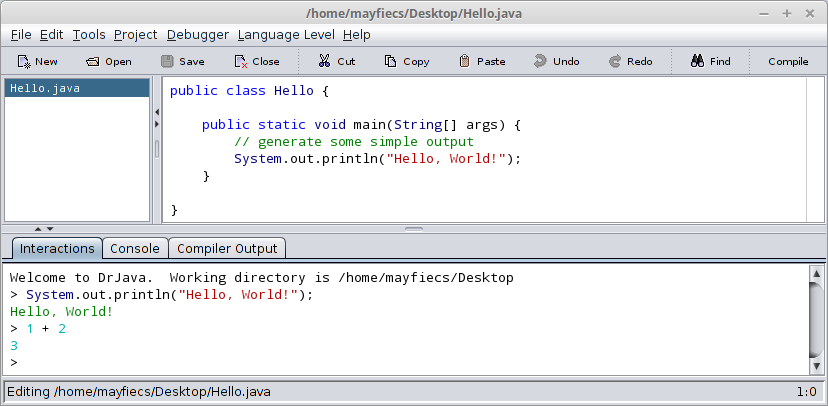
\includegraphics[width=\textwidth]{figs/drjava-hello.png}
\caption{Screenshot of DrJava editing the hello world program.}
\label{fig.drjava1}
\end{center}
\end{figure}

When running DrJava for the first time, we recommend you change three settings from the {\sf Edit $>$ Preferences} menu under {\sf Miscellaneous}: set the {\sf Indent Level} to 4, check the {\sf Automatically Close Block Comments} box, and uncheck the {\sf Keep Emacs-style Backup Files} box.

%We will use DrJava as the primary development environment throughout this book.

%Step-by-step instructions for installing the JDK and configuring DrJava are available on this book's website: \url{http://thinkjava.org/}.


\section{DrJava interactions}
\label{interactions}

One of the most useful features of DrJava is the ``Interactions Pane'' at the bottom of the window.
It provides the ability to try out code quickly, without having to write a class definition and save/compile/run the program.
Figure~\ref{fig.drjava2} shows an example.

\index{interactions}

\begin{figure}[!ht]
\begin{center}
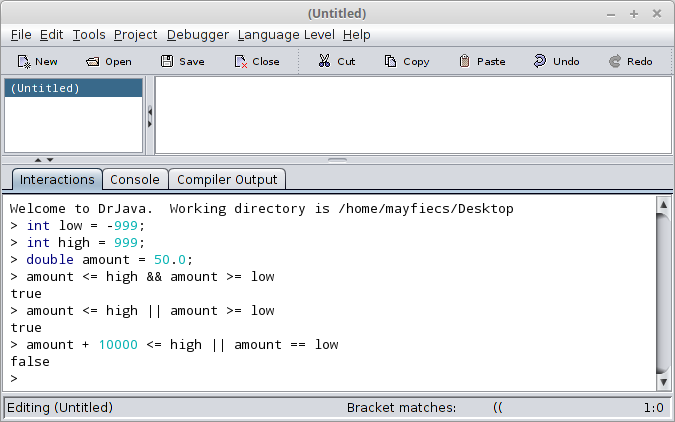
\includegraphics[width=\textwidth]{figs/drjava-logic.png}
\caption{Screenshot of the Interactions Pane in DrJava.}
\label{fig.drjava2}
\end{center}
\end{figure}

There is one subtle detail to note when using the Interactions feature.
If you don't end an expression (or statement) with a semicolon, DrJava automatically displays its value.
Notice in Figure~\ref{fig.drjava2} how the variable declarations end with semicolons, but the logic expressions in the following lines do not.
This feature saves you from having to type \java{System.out.println} every time.

What's nice about this feature is that you don't have to create a new class, declare a \java{main} method, write arbitrary expressions inside \java{System.out.println} statements, save the source file, and get all of your code to compile in advance.
Also, you can press the up/down arrows on the keyboard to repeat previous commands and experiment with incremental differences.


\section{Command-line interface}
\label{commandline}

\index{command-line interface}
\index{terminal}

One of the most powerful and useful skills you can learn is how to use the {\bf command-line interface}, also called the ``terminal''.
The command line is a direct interface to the operating system.
It allows you to run programs, manage files and directories, and monitor system resources.
Many advanced tools, both for software development and general-purpose computing, are available only at the command line.

There are many good tutorials online for learning the command line for your operating system; just search the web for ``command line tutorial''.
On Unix systems like Linux and OS X, you can get started with just four commands: change the working directory ({\tt cd}), list directory contents ({\tt ls}), compile Java programs ({\tt javac}), and run Java programs ({\tt java}).

Figure~\ref{fig.terminal} shows an example where the {\tt Hello.java} source file is stored in the {\tt Desktop} directory.
After changing to that location and listing the files, we use the {\tt javac} command to compile {\tt Hello.java}.
Running {\tt ls} again, we see that the compiler generated a new file, {\tt Hello.class}, which contains the byte code.
We run the program using the {\tt java} command, which displays the output on the following line.

\begin{figure}[!ht]
\begin{center}
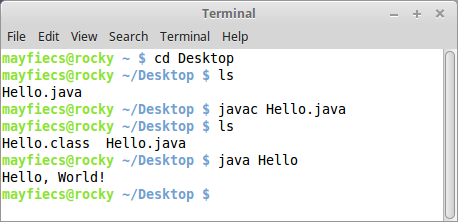
\includegraphics[width=4.5in]{figs/terminal.png}
\caption{Compiling and running {\tt Hello.java} from the command line.}
\label{fig.terminal}
\end{center}
\end{figure}

Note that the {\tt javac} command requires a {\em filename} (or multiple source files separated by spaces), whereas the {\tt java} command requires a single {\em class name}.
If you use DrJava, it runs these commands for you behind the scenes and displays the output in the Interactions Pane.

Taking time to learn this efficient and elegant way of interacting with the operating system will make you more productive.
People who don't use the command line don't know what they're missing.


\section{Command-line testing}
\label{cltesting}

\index{testing}

As described in Section~\ref{sec:examples}, it's more effective to program and debug your code little by little than to attempt writing everything all at once.
And after you've completed programming an algorithm, it's important to test that it works correctly on a variety of inputs.

Throughout the book, we illustrate techniques for testing your programs.
Most, if not all, testing is based on a simple idea: does the program do what we expect it to do?
For simple programs, it's not difficult to run them several times and see what happens.
But at some point, you will get tired of typing the same test cases over and over.

We can automate the process of entering input and comparing ``expected output'' with ``actual output'' using the command line.
The basic idea is to store the test cases in plain text files and trick Java into thinking they are coming from the keyboard.
Here are step-by-step instructions:

\begin{enumerate}

\item Make sure you can compile and run the {\tt Convert.java} example in the {\tt ch03} directory of {\tt ThinkJavaCode2}.

\item In the same directory as {\tt Convert.java}, create a plain text file named {\tt test.in} (``in'' is for input).
Enter the following line and save the file:

\begin{stdout}
193.04
\end{stdout}

\item Create a second plain text file named {\tt test.exp} (``exp'' is for expected).
Enter the following line and save the file:

\begin{stdout}
193.04 cm = 6 ft, 4 in
\end{stdout}

\item Open a terminal, and change to the directory with these files.
Run the following command to test the program:

\begin{stdout}
java Convert < test.in > test.out
\end{stdout}

\end{enumerate}

\index{redirection operator}
\index{operator!redirection}
\index{System.in}
\index{System.out}

On the command line, {\tt <} and {\tt >} are {\bf redirection operators}.
The first one redirects the contents of {\tt test.in} to \java{System.in}, as if it were entered from the keyboard.
The second one redirects the contents of \java{System.out} to a new file {\tt test.out}, much like a screen capture.
In other words, the {\tt test.out} file contains the output of your program.

By the way, it's perfectly okay to compile your programs in DrJava (or some other environment) and run them from the command line.
Knowing both techniques allows you to use the right tool for the job.

% CSM: moving fig.meld here so it's not in the middle of Checkstyle

\begin{figure}[!ht]
\begin{center}
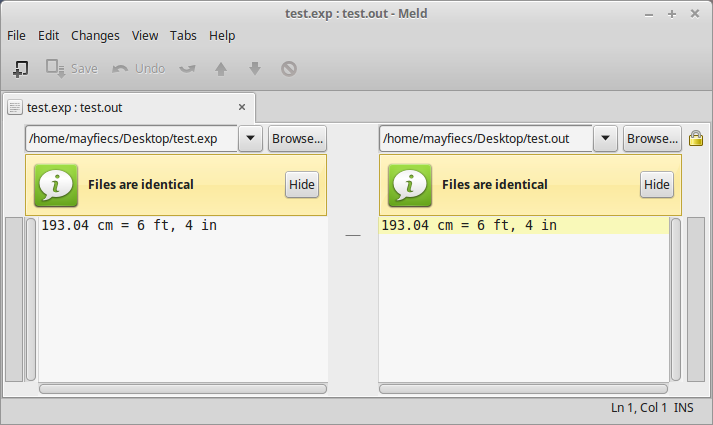
\includegraphics[width=0.9\textwidth]{figs/meld.png}
\caption{Using {\tt meld} to compare expected output with the actual output.}
\label{fig.meld}
\end{center}
\end{figure}

At this point, we just need to compare the contents {\tt test.out} with {\tt test.exp}.
If the files are the same, then the program outputted what we expected it to output.
If not, then we found a bug, and we can use the output to begin debugging our program.
Fortunately, there's a simple way to compare files on the command line:

\begin{stdout}
diff test.exp test.out
\end{stdout}

The {\tt diff} utility summarizes the differences between two files.
If there are no differences, then it displays nothing, which in our case is what we want.
If the expected output differs from the actual output, then we need to continue debugging.
Usually the program is at fault, and {\tt diff} provides some insight about what is broken.
But there's also a chance that we have a correct program and the expected output is wrong.

Interpreting the results from {\tt diff} can be confusing, but fortunately there are many graphical tools that show the differences between two files.
For example, on Windows you can install {\tt WinMerge}, on Mac you can use {\tt opendiff} (which comes with Xcode), and on Linux there's {\tt meld}, shown in Figure~\ref{fig.meld}.

Regardless of what tool you use, the goal is the same.
Debug your program until the actual output is {\em identical} to the expected output.


\section{Running Checkstyle}
\label{checkstyle}

\index{Checkstyle}

Checkstyle is a command-line tool that can be used to determine if your source code follows a set of style rules.
It also checks for common programming mistakes, such as class and method design problems.

You can download the latest version as a JAR file from \url{http://checkstyle.sourceforge.net/}.
To run Checkstyle, move (or copy) the JAR file to the same directory as your program.
Open a terminal in that location, and run the following command:

\begin{stdout}
java -jar checkstyle-*-all.jar -c /google_checks.xml *.java
\end{stdout}

\index{wildcard}

The {\tt *} characters are {\bf wildcards} that match whatever version of Checkstyle you have and whatever Java source files are present.
The output indicates the file and line number of each problem.
This example refers to a method beginning on line 93, column 5 of {\tt Hello.java}:

\begin{stdout}
Hello.java:93:5: Missing a Javadoc comment
\end{stdout}

The file \java{/google_checks.xml} is inside the JAR file and represents most of Google's style rules.
You can alternatively use \java{/sun_checks.xml} or provide your own configuration file.
See Checkstyle's website for more information.

If you apply Checkstyle to your source code often, you will likely internalize good style habits over time.
But there are limits to what automatic style checkers can do.
In particular, they can't evaluate the {\em quality} of your comments, the {\em meaning} of your variable names, or the {\em structure} of your algorithms.

Good comments make it easier for experienced developers to identify errors in your code.
Good variable names communicate the intent of your program and how the data is organized.
And good programs are designed to be efficient and demonstrably correct.


\section{Tracing with a debugger}
\label{debugger}

\index{debugger}

A great way to visualize the flow of execution, including how parameters and arguments work, is to use a {\bf debugger}.
Most debuggers make it possible to:

\index{breakpoint}

\begin{enumerate}
\item Set a {\bf breakpoint}, a line where you want the program to pause.
\item Step through the code one line at a time and watch what it does.
\item Check the values of variables and see when and how they change.
\end{enumerate}

For example, open any program in DrJava and move the cursor to the first line of \java{main}.
Press {\sf Ctrl+B} to toggle a breakpoint on the current line; it should now be highlighted in red.
Press {\sf Ctrl+Shift+D} to turn on Debug Mode; a new pane should appear at the bottom of the window.
These commands are also available from the {\sf Debugger} menu, in case you forget the shortcut keys.

\index{call stack}

When you run the program, execution pauses at the first breakpoint.
The debug pane displays the {\bf call stack}, with the current method on top of the stack, as shown in Figure~\ref{fig.debugger}.
You might be surprised to see how many methods were called before the \java{main} method!

\begin{figure}[!ht]
\begin{center}
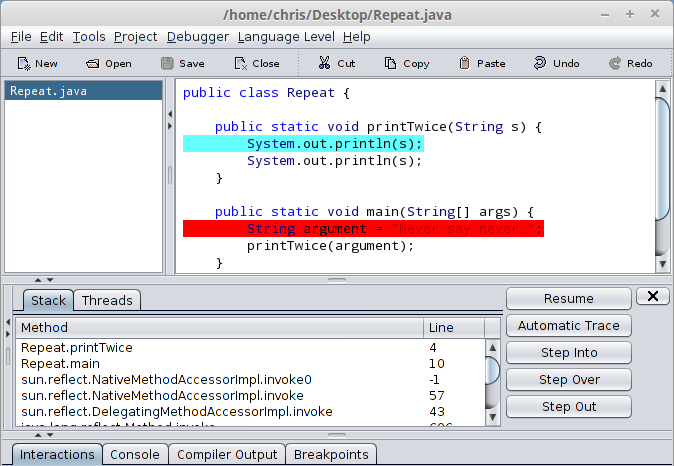
\includegraphics[width=\textwidth]{figs/debugger.png}
\caption{Screenshot of the DrJava debugger.
Execution is currently paused on the first line of \java{printTwice}.
There is a breakpoint on the first line of \java{main}.}
\label{fig.debugger}
\end{center}
\end{figure}

\index{tracing}

To the right are several buttons that allow you to step through the code at your own pace.
You can also press {\sf Automatic Trace} to watch DrJava run your code one line at a time.

Using a debugger is like having the computer proofread your code out loud.
When the program is paused, you can examine (or even change) the value of any variable using the Interactions Pane.

Tracing allows you to follow the flow of execution and see how data pass from one method to another.
You might expect the code do one thing, but then the debugger shows it doing something else.
At that moment, you gain insight about what may be wrong with the code.

You can edit your code while debugging it, but we don't recommend it.
If you add or delete multiple lines of code while the program is paused, the results can be confusing.

See \url{http://drjava.org/docs/user/ch09.html} for more information about using the debugger feature of DrJava.


\section{Testing with JUnit}
\label{JUnit}

\index{unit test}

When beginners start writing methods, they usually test them by invoking them from \java{main} and checking the results by hand.
Writing code like this can get repetitive, but there are tools to make it easier.
For cases where we know the right answer, we can do better by writing {\bf unit tests}.

For example, to test \java{fibonacci} from Section~\ref{fibonacci}, we could write:

\begin{code}
public static void main(String[] args) {
    if (fibonacci(1) != 1) {
        System.err.println("fibonacci(1) is incorrect");
    }
    if (fibonacci(2) != 1) {
        System.err.println("fibonacci(2) is incorrect");
    }
    if (fibonacci(3) != 2) {
        System.err.println("fibonacci(3) is incorrect");
    }
}
\end{code}

This test code is self-explanatory, but it's longer than it needs to be and it doesn't scale very well.
In addition, the error messages provide limited information.
Using a unit test framework addresses these and other issues.

JUnit is a common testing tool for Java programs (see \url{http://junit.org/}).
To use it, you have to create a test class that contains test methods.
If the name of your class is \java{Class}, the name of the test class is \java{ClassTest}.
And if there is a method in \java{Class} named \java{method}, there should be a method in \java{TestClass} named \java{testMethod}.

For example, suppose that the \java{fibonacci} method belongs to a class named \java{Series}.
Here is the corresponding JUnit test class and test method:

\begin{code}
import junit.framework.TestCase;

public class SeriesTest extends TestCase {

    public void testFibonacci() {
        assertEquals(1, Series.fibonacci(1));
        assertEquals(1, Series.fibonacci(2));
        assertEquals(2, Series.fibonacci(3));
    }
}
\end{code}

This example uses the keyword \java{extends}, which indicates that the new class, \java{SeriesTest} is based on an existing class, \java{TestCase}.
The \java{TestCase} class is imported from the package \java{junit.framework}.

Many development environments can generate test classes and test methods automatically.
In DrJava, you can select {\sf New JUnit Test Case} from the {\sf File} menu to generate an empty test class.

\java{assertEquals} is provided by the \java{TestCase} class.
It takes two arguments and checks whether they are equal.
If so, it does nothing; otherwise it displays a detailed error message.
The first argument is the ``expected value'', which we consider correct, and the second argument is the ``actual value'' we want to check.
If they are not equal, the test fails.

\index{System.err}

Using \java{assertEquals} is more concise than writing your own \java{if} statements and \java{System.err} messages.
JUnit provides additional assert methods, such as \java{assertNull}, \java{assertSame}, and \java{assertTrue}, that can be used to design a variety of tests.

To run JUnit directly from DrJava, click the {\sf Test} button on the toolbar.
If all your test methods pass, you will see a green bar in the lower-right corner.
Otherwise, DrJava will take you directly to the first assertion that failed.


\section{Vocabulary}

\begin{description}

\term{IDE}
An ``integrated development environment'' that includes tools for editing, compiling, and debugging programs.

\term{JDK}
The ``Java Development Kit'' that contains the compiler, Javadoc, and other tools.

\term{JVM}
The ``Java Virtual Machine'' that interprets the compiled byte code.

\term{text editor}
A program that edits plain text files, the format used by most programming languages.

\term{JAR}
A ``Java Archive'', which is essentially a ZIP file containing classes and other resources.

\term{command-line interface}
A means of interacting with the computer by issuing commands in the form of successive lines of text.

\term{redirection operator}
A command-line feature that substitutes \java{System.in} and/or \java{System.out} with a plain text file.

\term{wildcard}
A command-line feature that allows you to specify a pattern of filenames using the {\tt *} character.

\term{debugger}
A tool that allows you to run one statement at a time and see the contents of variables.

\term{breakpoint}
A line of code where the debugger will pause a running program.

\term{call stack}
The history of method calls and where to resume execution after each method returns.

\term{unit test}
Code that exercises a single method of a program, testing for correctness and/or efficiency.

\end{description}


\chapter{Javadoc}
\label{javadoc}

\index{comment!end-of-line}
\index{comment!multi-line}
\index{comment!documentation}

Java programs have three different types of comments:

\begin{enumerate}
\item {\bf End-of-line comments} (\java{//}), which generally contain short phrases that explain specific lines of code.
\item {\bf Multi-line comments} (\java{/*}), which are typically only used for copyright statements at the top of the file.
\item {\bf Documentation comments} (\java{/**}), which describe in sufficient detail what each class and method does.
\end{enumerate}

End-of-line and multi-line comments are written primarily for yourself.
They help you remember specific details about your source code.
Documentation comments, on the other hand, are written for others.
They explain how to use your classes and methods in other programs.

\index{HTML}
\index{Javadoc}

A nice feature of the Java language is the ability to embed documentation in the source code itself.
That way, you can write it as you go, and as things change, it is easier to keep the documentation consistent with the code.

You can extract documentation from your source code, and generate well-formatted HTML pages, using a tool called {\bf Javadoc}.
This tool is included with the Java compiler, and it is widely used.
In fact, the official documentation for the Java library (\url{https://docs.oracle.com/javase/8/docs/api/}) is generated by Javadoc.


\section{Reading documentation}

\index{documentation}

%One of the nice things about Java is that it comes with an extensive library of classes and methods.
%But before you use them, you might have to read the documentation.
%And sometimes that's not easy.

As an example, let's look at the documentation for \java{Scanner}, a class we first used in Section~\ref{scanner}.
You can find the documentation quickly by doing a web search for ``Java Scanner''.
Figure~\ref{fig.scanner} shows a screenshot of the page.

\begin{figure}[!ht]
\begin{center}
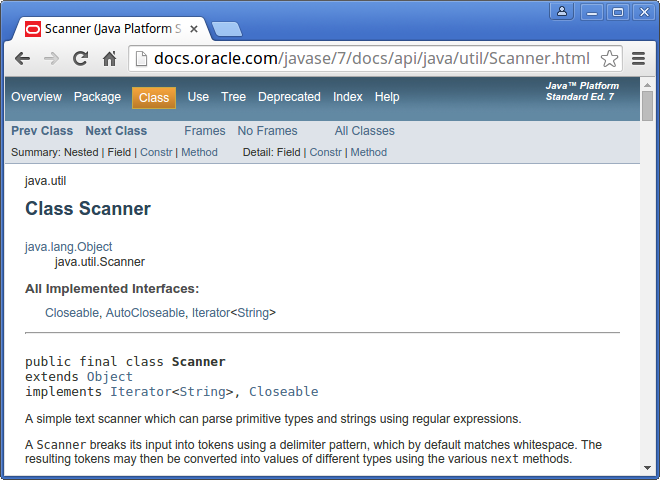
\includegraphics[width=0.9\textwidth]{figs/scanner.png}
\caption{Screenshot of the documentation for \java{Scanner}.}
\label{fig.scanner}
\end{center}
\end{figure}

Documentation for other classes uses a similar format.
The first line is the package that contains the class, such as \java{java.util}.
The second line is the name of the class.
The ``Implemented Interfaces'' section lists some of the functionality a \java{Scanner} has.
%; we won't say more about that for now.

%The next two lines indicate that every \java{Scanner} is also an \java{Object}; that will make more sense after Section~\ref{inheritance}.

The next section of the documentation is a narrative that explains the purpose of the class and includes examples of how to use it.
This text can be difficult to read, because it may use terms you have not yet learned.
But the examples are often very useful.
A good way to get started with a new class is to paste the examples into a test file and see if you can compile and run them.

One of the examples shows how you can use a \java{Scanner} to read input from a \java{String} instead of \java{System.in}:

%NOTE: only use of Scanner w/o System.in; mention this again in String chapter?
\begin{code}
String input = "1 fish 2 fish red fish blue fish";
Scanner s = new Scanner(input);
\end{code}

After the narrative, code examples, and some other details, you will find the following tables:

\begin{description}

\item[Constructor summary:]
Ways of creating, or ``constructing'', a \java{Scanner}.

\item[Method summary:]
The list of methods that the \java{Scanner} class provides.

\item[Constructor detail:]
More information about how to create a \java{Scanner}.

\item[Method detail:]
More information about each method.

\end{description}

For example, here is the summary information for \java{nextInt}:

\begin{stdout}
public int nextInt()
Scans the next token of the input as an int.
\end{stdout}

\index{signature}

The first line is the method's {\bf signature}, which specifies the name of the method, its parameters (none), and what type it returns (\java{int}).
The next line is a short description of what it does.

The ``Method detail'' explains more:

\begin{stdout}
public int nextInt()
Scans the next token of the input as an int.

An invocation of this method of the form nextInt() behaves in
exactly the same way as the invocation nextInt(radix), where
radix is the default radix of this scanner.

Returns:
the int scanned from the input

Throws:
InputMismatchException - if the next token does not match
    the Integer regular expression, or is out of range
NoSuchElementException - if input is exhausted
IllegalStateException - if this scanner is closed
\end{stdout}

The ``Returns'' section describes the result when the method succeeds.
In contrast, the ``Throws'' section describes possible errors and exceptions that may occur.
Exceptions are said to be ``thrown'', like a referee throwing a flag, or like a toddler throwing a fit.

It might take you some time to get comfortable reading documentation and learning which parts to ignore.
But it's worth the effort.
Knowing what's available in the library helps you avoid reinventing the wheel.
And a little bit of documentation can save you a lot of debugging.


\section{Writing documentation}

As you benefit from reading good documentation, you should ``pay it forward'' by writing good documentation.

\index{comment!documentation}
\index{documentation!Javadoc comments}

Javadoc scans your source files looking for documentation comments, also known as ``Javadoc comments''.
They begin with \java{/**} (two stars) and end with \textcolor{comment}{\tt */} (one star).
Anything in between is considered part of the documentation.

Here's a class definition with two Javadoc comments, one for the \java{Goodbye} class and one for the \java{main} method:

\begin{code}
/**
 * Example program that demonstrates print vs println.
 */
public class Goodbye {

    /**
     * Prints a greeting.
     */
    public static void main(String[] args) {
        System.out.print("Goodbye, ");  // note the space
        System.out.println("cruel world");
    }
}
\end{code}

The class comment explains the purpose of the class.
The method comment explains what the method does.

Notice that this example also has an end-of-line comment (\java{//}).
In general, these comments are short phrases that help explain complex parts of a program.
They are intended for other programmers reading and maintaining the source code.

In contrast, Javadoc comments are longer, usually complete sentences.
They explain what each method does, but they omit details about how the method works.
And they are intended for people who will use the methods without looking at the source code.

Appropriate comments and documentation are essential for making source code readable.
And remember that the person most likely to read your code in the future, and appreciate good documentation, is you.


\section{Javadoc tags}

%In Section~\ref{sec:javadoc}, we discussed how to write documentation comments using \java{/**}.
It's generally a good idea to document each class and method, so that other programmers can understand what they do without having to read the code.

\index{tag}
\index{param tag}
\index{return tag}
\index{documentation!Javadoc tags}

To organize the documentation into sections, Javadoc supports optional {\bf tags} that begin with the at sign (\java{@}).
For example, we can use \java{@author} and \java{@version} to provide information about the class.

\begin{code}
/**
 * Utility class for extracting digits from integers.
 *
 * @author Chris Mayfield
 * @version 1.0
 */
public class DigitUtil {
\end{code}

\index{description}

Documentation comments should begin with a {\bf description} of the class or method, followed by the tags.
These two sections are separated by a blank line (not counting the \textcolor{comment}{\tt *}).

For methods, we can use \java{@param} and \java{@return} to provide information about parameters and return values.

\begin{code}
/**
 * Tests whether x is a single digit integer.
 *
 * @param x the integer to test
 * @return true if x has one digit, false otherwise
 */
public static boolean isSingleDigit(int x) {
\end{code}

\index{HTML}
\index{Javadoc}

Figure~\ref{fig.javadoc} shows part of the resulting HTML page generated by Javadoc.
Notice the relationship between the Javadoc comment (in the source code) and the resulting documentation (in the HTML page).

\begin{figure}[!ht]
\begin{center}
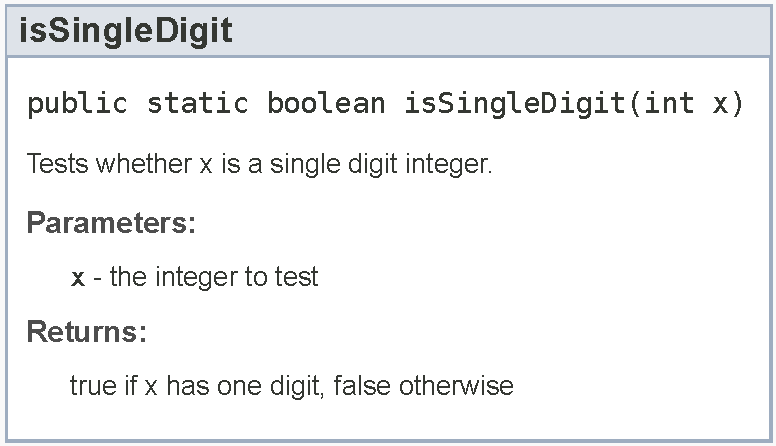
\includegraphics[scale=0.8]{figs/javadoc.pdf}
\caption{HTML documentation for \java{isSingleDigit}.}
\label{fig.javadoc}
\end{center}
\end{figure}

When writing parameter comments, do not include a hyphen (\java{-}) after the \java{@param} tag.
Otherwise, you will have two hyphens in the resulting HTML documentation.

Notice also that the \java{@return} tag should not specify the type of the method.
Comments like \textcolor{comment}{\tt @return boolean} are not useful, because you already know the return type from the method's signature.

Methods with multiple parameters should have separate \java{@param} tags that describe each one.
Void methods should have no \java{@return} tag, since they do not return a value.
Each tag should be on its own line in the source code.


\section{Example source file}

Now let's take a look at a more complete example.
The code for this section is in the {\tt appb} directory of {\tt ThinkJavaCode2}.
See page~\pageref{code} for instructions on how to download the repository.

Professional-grade source files often begin with a copyright statement.
This text spans multiple lines, but it is not part of the documentation.
So we use a multi-line comment (\java{/*}).
Our example source file, {\tt Convert.java}, includes the MIT License (\url{https://opensource.org/licenses/MIT}).

\index{Convert.java}

\begin{scriptsize}
\begin{code}
/*
 * Copyright (c) 2017 Allen Downey and Chris Mayfield
 *
 * Permission is hereby granted, free of charge, to any person obtaining a copy
 * of this software and associated documentation files (the "Software"), to deal
 * in the Software without restriction, including without limitation the rights
 * to use, copy, modify, merge, publish, distribute, sublicense, and/or sell
 * copies of the Software, and to permit persons to whom the Software is
 * furnished to do so, subject to the following conditions:
 *
 * The above copyright notice and this permission notice shall be included in
 * all copies or substantial portions of the Software.
 *
 * THE SOFTWARE IS PROVIDED "AS IS", WITHOUT WARRANTY OF ANY KIND, EXPRESS OR
 * IMPLIED, INCLUDING BUT NOT LIMITED TO THE WARRANTIES OF MERCHANTABILITY,
 * FITNESS FOR A PARTICULAR PURPOSE AND NONINFRINGEMENT. IN NO EVENT SHALL THE
 * AUTHORS OR COPYRIGHT HOLDERS BE LIABLE FOR ANY CLAIM, DAMAGES OR OTHER
 * LIABILITY, WHETHER IN AN ACTION OF CONTRACT, TORT OR OTHERWISE, ARISING FROM,
 * OUT OF OR IN CONNECTION WITH THE SOFTWARE OR THE USE OR OTHER DEALINGS IN THE
 * SOFTWARE.
 */
\end{code}
\end{scriptsize}

%This program uses a \java{Scanner}, so we have to \java{import} it.
Import statements generally follow the copyright text.
After that, we can define the class itself and begin writing the documentation (\java{/**}).

\begin{code}
import java.util.Scanner;

/**
 * Methods for converting to/from the metric system.
 *
 * @author Allen Downey
 * @author Chris Mayfield
 * @version 6.1.5
 */
public class Convert {
\end{code}

A common mistake that beginners make is to put \java{import} statements between the documentation and the \java{public class} line.
Doing so separates the documentation from the class itself.
To avoid this issue, always make the end of the comment (the \textcolor{comment}{\tt */}) ``touch'' the word \java{public}.


This class has two constants and three methods.
The constants are self-explanatory, so there is no need to write documentation for them.

\begin{code}
public static final double CM_PER_INCH = 2.54;

public static final int IN_PER_FOOT = 12;
\end{code}

The methods, on the other hand, could use some explanation.
Each documentation comment includes a description, followed by a blank line, followed by a \java{@param} tag for each parameter, followed by a \java{@return} tag.

\begin{code}
/**
 * Converts a measurement in centimeters to inches.
 *
 * @param cm length in centimeters
 * @return length in inches
 */
public static double toImperial(double cm) {
    return cm / CM_PER_INCH;
}

/**
 * Converts a length in feet and inches to centimeters.
 *
 * @param feet how many feet
 * @param inches how many inches
 * @return length in centimeters
 */
public static double toMetric(int feet, int inches) {
    int total = feet * IN_PER_FOOT + inches;
    return total * CM_PER_INCH;
}
\end{code}

The \java{main} method has a similar documentation comment, except there is no \java{@return} tag since the method is \java{void}.
%And because it's longer than a few lines, it includes end-of-line comments (\java{//}) as well.

\begin{code}
/**
 * Tests the conversion methods.
 *
 * @param args command-line arguments
 */
public static void main(String[] args) {
    double cm, result;
    int feet, inches;
    Scanner in = new Scanner(System.in);

    // test the Imperial conversion
    System.out.print("Exactly how many cm? ");
    cm = in.nextDouble();
    result = toImperial(cm);
    System.out.printf("That's %.2f inches\n", result);
    System.out.println();

    // test the Metric conversion
    System.out.print("Now how many feet? ");
    feet = in.nextInt();
    System.out.print("And how many inches? ");
    inches = in.nextInt();
    result = toMetric(feet, inches);
    System.out.printf("That's %.2f cm\n", result);
}
\end{code}

Here are two ways you can run the Javadoc tool on this example program:

\begin{enumerate}

\index{command-line interface}

\item From the command line, go to the location for {\tt Convert.java}.
The {\tt -d} option of {\tt javadoc} indicates where to generate the HTML files.

\begin{stdout}
javadoc -d doc Convert.java
\end{stdout}

\item From DrJava, click the {\sf Javadoc} button on the toolbar.
The IDE will then prompt you for a location to generate the HTML files.
\end{enumerate}

For more examples of what you can do with Javadoc comments, see the source code of any Java library class (e.g., {\tt Scanner.java}).
Section~\ref{src.zip} explains how to find the source files for the Java library on your computer.


\section{Vocabulary}

\begin{description}

\term{documentation}
Comments that describe the technical operation of a class or method.

\term{Javadoc}
A tool that reads Java source code and generates documentation in HTML format.

\term{signature}
The first line of a method that defines its name, return type, and parameters.

\term{tag}
A label that begins with an at sign (\java{@}) and is used by Javadoc to organize documentation into sections.

\term{description}
The first line of a documentation comment that explains what the class/method does.

\end{description}


\chapter{Graphics}
\label{graphics}

\index{AWT}
\index{java.awt}

The Java library includes a simple package for drawing 2D graphics, called \java{java.awt}.
{\bf AWT} stands for ``Abstract Window Toolkit''.
We are only going to scratch the surface of graphics programming; you can read more about it in the Java tutorials at \url{https://docs.oracle.com/javase/tutorial/2d/}.


\section{Creating graphics}

\index{Canvas}
\index{class!Canvas}
\index{Graphics}
\index{class!Graphics}

There are several ways to create graphics in Java; the simplest way is to use \java{java.awt.Canvas} and \java{java.awt.Graphics}.
A \java{Canvas} is a blank rectangular area of the screen onto which the application can draw.
The \java{Graphics} class provides basic drawing methods such as \java{drawLine}, \java{drawRect}, and \java{drawString}.

Here is an example program that draws a circle using the \java{fillOval} method:

\begin{code}
import java.awt.Canvas;
import java.awt.Graphics;
import javax.swing.JFrame;

public class Drawing extends Canvas {
\end{code}

\begin{code}
    public static void main(String[] args) {
        JFrame frame = new JFrame("My Drawing");
        Canvas canvas = new Drawing();
        canvas.setSize(400, 400);
        frame.add(canvas);
        frame.pack();
        frame.setVisible(true);
    }

    public void paint(Graphics g) {
        g.fillOval(100, 100, 200, 200);
    }
}
\end{code}

The \java{Drawing} class extends \java{Canvas}, so it has all the methods provided by \java{Canvas}, including \java{setSize}.
You can read about the other methods in the documentation, which you can find by doing a web search for ``Java Canvas''.

\index{JFrame}
\index{class!JFrame}

In the \java{main} method, we:

\begin{enumerate}

\item Create a \java{JFrame} object, which is the window that will contain the canvas.

\item Create a \java{Drawing} object (which is the canvas), set its width and height, and add it to the frame.

\item Pack the frame (resize it) to fit the canvas, and display it on the screen.
\end{enumerate}

\index{paint}

Once the frame is visible, the \java{paint} method is called whenever the canvas needs to be drawn; for example, when the window is moved or resized.
The application doesn't end after the \java{main} method returns; instead, it waits for the \java{JFrame} to close.
If you run this code, you should see a black circle on a gray background.


\section{Graphics methods}

\index{coordinate}
\index{pixel}

You are probably used to Cartesian {\bf coordinates}, where $x$ and $y$ values can be positive or negative.
In contrast, Java uses a coordinate system where the origin is in the upper-left corner.
That way, $x$ and $y$ are always positive integers.
Figure~\ref{fig.coordinates} shows these coordinate systems.

Graphical coordinates are measured in {\bf pixels}; each pixel corresponds to a dot on the screen.

\begin{figure}[!ht]
\begin{center}
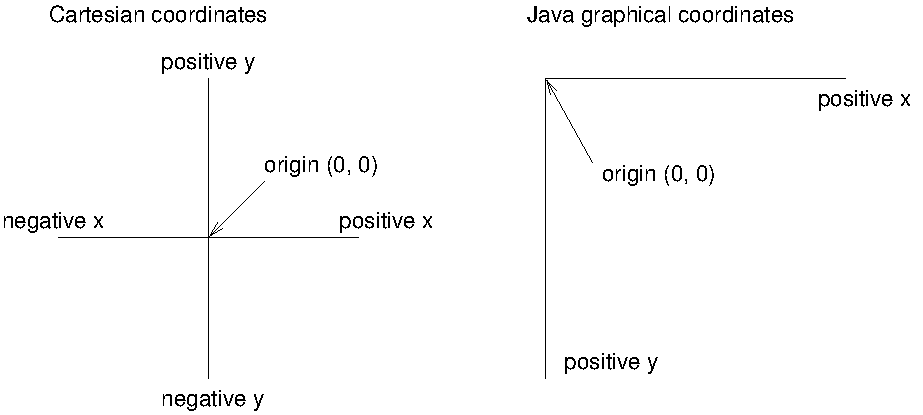
\includegraphics[width=5in]{figs/coordinates.pdf}
\caption{Diagram of the difference between Cartesian coordinates and Java graphical coordinates.}
\label{fig.coordinates}
\end{center}
\end{figure}

To draw on the canvas, you invoke methods on a \java{Graphics} object.
You don't have to create the \java{Graphics} object; it gets created when you create the \java{Canvas}, and it gets passed as an argument to \java{paint}.

The previous example used \java{fillOval}, which has the following signature:

\begin{code}
/**
 * Fills an oval bounded by the specified rectangle with
 * the current color.
 */
public void fillOval(int x, int y, int width, int height)
\end{code}

\index{bounding box}

The four parameters specify a {\bf bounding box}, which is the rectangle in which the oval is drawn.
\java{x} and \java{y} specify the location of the upper-left corner of the bounding box.
The bounding box itself is not drawn (see Figure~\ref{fig.circle}).

\begin{figure}[!ht]
\begin{center}
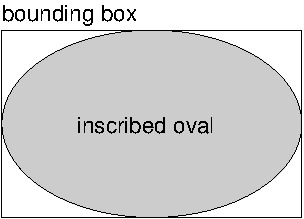
\includegraphics{figs/circle.pdf}
\caption{Diagram of an oval inside its bounding box.}
\label{fig.circle}
\end{center}
\end{figure}

\index{Color}

To choose the color of a shape, invoke \java{setColor} on the \java{Graphics} object:

\begin{code}
g.setColor(Color.red);
\end{code}

The \java{setColor} method determines the color of everything that gets drawn afterward.
\java{Color.red} is a constant provided by the \java{Color} class; to use it you have to \java{import java.awt.Color}.
Other colors include:

\begin{stdout}
black       blue      cyan     darkGray   gray    green
lightGray   magenta   orange   pink       white   yellow
\end{stdout}

\index{RGB}

You can create your own colors by specifying the red, green, and blue ({\bf RGB}) components.
For example:

\begin{code}
Color purple = new Color(128, 0, 128);
\end{code}

Each value is an integer in the range 0 (darkest) to 255 (lightest).
The color \java{(0, 0, 0)} is black, and \java{(255, 255, 255)} is white.

You can set the background color of the \java{Canvas} by invoking \java{setBackground}:

\begin{code}
canvas.setBackground(Color.white);
\end{code}


\section{Example drawing}

\index{Mickey Mouse}

Suppose we want to draw a ``Hidden Mickey'', which is an icon that represents Mickey Mouse (see \url{https://en.wikipedia.org/wiki/Hidden_Mickey}).
We can use the oval we just drew as the face, and then add two ears.
To make the code more readable, let's use \java{Rectangle} objects to represent bounding boxes.

Here's a method that takes a \java{Rectangle} and invokes \java{fillOval}:

\begin{code}
public void boxOval(Graphics g, Rectangle bb) {
    g.fillOval(bb.x, bb.y, bb.width, bb.height);
}
\end{code}

And here's a method that draws Mickey Mouse:

\begin{code}
public void mickey(Graphics g, Rectangle bb) {
    boxOval(g, bb);

    int dx = bb.width / 2;
    int dy = bb.height / 2;
    Rectangle half = new Rectangle(bb.x, bb.y, dx, dy);

    half.translate(-dx / 2, -dy / 2);
    boxOval(g, half);

    half.translate(dx * 2, 0);
    boxOval(g, half);
}
\end{code}

The first line draws the face.
The next three lines create a smaller rectangle for the ears.
We \java{translate} the rectangle up and left for the first ear, then to the right for the second ear.
The result is shown in Figure~\ref{fig.mickey}.

\begin{figure}[!ht]
\begin{center}

\includegraphics[height=2in]{figs/mickey.png}
\caption{A ``Hidden Mickey'' drawn using Java graphics.}
\label{fig.mickey}
\end{center}
\end{figure}

You can read more about \java{Rectangle} and \java{translate} in Chapter~\ref{mutable}.
See the exercises at the end of this appendix for more example drawings.


\section{Vocabulary}

\begin{description}

\term{AWT}
The ``Abstract Window Toolkit'', a Java package for creating graphical user interfaces.

\term{coordinate}
A value that specifies a location in a 2D graphical window.

\term{pixel}
The unit in which coordinates are measured.

\term{bounding box}
A way to specify the coordinates of a rectangular area.

\term{RGB}
A color model based on adding red, green, and blue light.

\end{description}


\section{Exercises}

The code for this chapter is in the {\tt appc} directory of {\tt ThinkJavaCode2}.
See page~\pageref{code} for instructions on how to download the repository.
Before you start the exercises, we recommend that you compile and run the examples.


\begin{exercise}

Draw the flag of Japan: a red circle on a white background that is wider than it is tall.

\end{exercise}


\begin{exercise}

Modify {\tt Mickey.java} to draw ears on the ears, and ears on those ears, and more ears all the way down until the smallest ears are only 3 pixels wide.
The result should look like ``Mickey Moose'', shown in Figure~\ref{fig.moose}.
{\it Hint:} You should only have to add or modify a few lines of code.

\begin{figure}[!ht]
\begin{center}
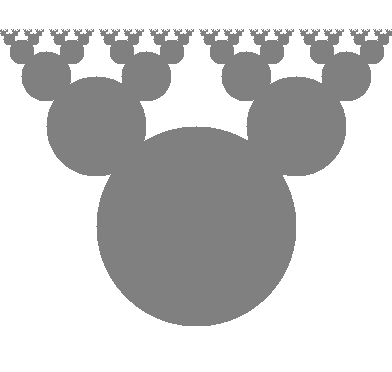
\includegraphics[height=2in]{figs/moose.png}
\caption{A recursive shape we call ``Mickey Moose''.}
\label{fig.moose}
\end{center}
\end{figure}

\end{exercise}


\begin{exercise}

In this exercise, you will draw ``Moir\'{e} patterns'' that seem to shift around as you move.
For an explanation of what is going on, see \url{https://en.wikipedia.org/wiki/Moire_pattern}.

\begin{enumerate}

\item Open {\tt Moire.java} and read the \java{paint} method.
Draw a sketch of what you expect it to do.
Now run it.
Did you get what you expected?

\item Modify the program so that the space between the circles is larger or smaller.
See what happens to the image.

\item Modify the program so that the circles are drawn in the center of the screen and concentric, as in Figure~\ref{fig.moire} (left).
The distance between the circles should be small enough that the Moir\'{e} interference is apparent.

\begin{figure}[!ht]
\begin{center}
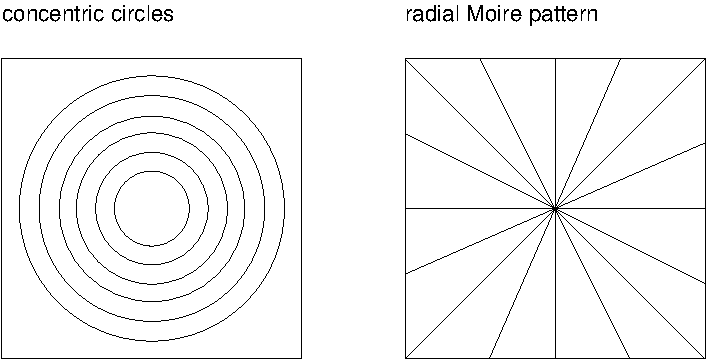
\includegraphics[height=2in]{figs/moire.pdf}
\caption{Graphical patterns that can exhibit Moir\'{e} interference.}
\label{fig.moire}
\end{center}
\end{figure}

\item Write a method named \java{radial} that draws a radial set of line segments as shown in Figure~\ref{fig.moire} (right), but they should be close enough together to create a Moir\'{e} pattern.

\item Just about any kind of graphical pattern can generate Moir\'{e}-like interference patterns.
Play around and see what you can create.

\end{enumerate}

\end{exercise}


\chapter{Debugging}
\label{debugging}

\index{debugging}

Although there are debugging suggestions throughout the book, we thought it would be useful to organize them in an appendix.
If you are having a hard time debugging, you might want to review this appendix from time to time.

The best debugging strategy depends on what kind of error you have:

\begin{itemize}

\item {\bf Compile-time errors} indicate that there is something wrong with the syntax of the program.
Example: omitting the semicolon at the end of a statement.

\index{compile-time error}
\index{error!compile-time}
\index{syntax}

\item {\bf Run-time errors} are produced if something goes wrong while the program is running.
Example: an infinite recursion eventually causes a \java{StackOverflowError}.

\index{run-time error}
\index{error!run-time}
\index{exception}

\item {\bf Logic errors} cause the program to do the wrong thing.
Example: an expression may not be evaluated in the order you expect.

\index{logic error}
\index{error!logic}

\end{itemize}

The following sections are organized by error type; some techniques are useful for more than one type.


\section{Compile-time errors}

The best kind of debugging is the kind you don't have to do because you avoid making errors in the first place.
Incremental development, which we presented in Section~\ref{distance}, can help.
The key is to start with a working program and add small amounts of code at a time.
When there is an error, you will have a pretty good idea where it is.

Nevertheless, you might find yourself in one of the following situations.
For each situation, we have some suggestions about how to proceed.


\subsection*{The compiler is spewing error messages.}

\index{compile}
\index{error!message}

If the compiler reports 100 error messages, that doesn't mean there are 100 errors in your program.
When the compiler encounters an error, it often gets thrown off track for a while.
It tries to recover and pick up again after the first error, but sometimes it reports spurious errors.

Only the first error message is truly reliable.
We suggest that you only fix one error at a time, and then recompile the program.
You may find that one semicolon or brace ``fixes'' 100 errors.


\subsection*{I'm getting a weird compiler message, and it won't go away.}

First of all, read the error message carefully.
It may be written in terse jargon, but often there is a carefully hidden kernel of information.

If nothing else, the message will tell you where in the program the problem occurred.
Actually, it tells you where the compiler was when it noticed a problem, which is not necessarily where the error is.
Use the information the compiler gives you as a guideline, but if you don't see an error where the compiler is pointing, broaden the search.

Generally the error will be prior to the location of the error message, but there are cases where it will be somewhere else entirely.
For example, if you get an error message at a method invocation, the actual error may be in the method definition itself.

If you don't find the error quickly, take a breath and look more broadly at the entire program.
Make sure the program is indented properly; that makes it easier to spot syntax errors.

Now, start looking for common syntax errors:

\index{syntax errors}
\index{error!syntax}

\begin{enumerate}

\item Check that all parentheses and brackets are balanced and properly nested.
All method definitions should be nested within a class definition.
All program statements should be within a method definition.

\item Remember that uppercase letters are not the same as lowercase letters.

\item Check for semicolons at the end of statements (and no semicolons after curly braces).

\index{quote mark}

\item Make sure that any strings in the code have matching quotation marks.
Make sure that you use double quotes for strings and single quotes for characters.

\item For each assignment statement, make sure that the type on the left is the same as the type on the right.
Make sure that the expression on the left is a variable name or something else that you can assign a value to (like an element of an array).

\item For each method invocation, make sure that the arguments you provide are in the right order and have the right type, and that the object you are invoking the method on is the right type.

\item If you are invoking a value method, make sure you are doing something with the result.
If you are invoking a void method, make sure you are {\em not} trying to do something with the result.

\item If you are invoking an instance method, make sure you are invoking it on an object with the right type.
If you are invoking a static method from outside the class where it is defined, make sure you specify the class name (using dot notation).

\item Inside an instance method you can refer to the instance variables without specifying an object.
If you try that in a static method -- with or without \java{this} -- you get a message like ``non-static variable x cannot be referenced from a static context.''

\end{enumerate}

If nothing works, move on to the next section...


\subsection*{I can't get my program to compile no matter what I do.}

If the compiler says there is an error and you don't see it, that might be because you and the compiler are not looking at the same code.
Check your development environment to make sure the program you are editing is the program the compiler is compiling.

This situation is often the result of having multiple copies of the same program.
You might be editing one version of the file, but compiling a different version.

If you are not sure, try putting an obvious and deliberate syntax error right at the beginning of the program.
Now compile again.
If the compiler doesn't find the new error, there is probably something wrong with the way you set up the development environment.

\index{debugging!by bisection}

If you have examined the code thoroughly, and you are sure the compiler is compiling the right source file, it is time for desperate measures: {\bf debugging by bisection}.

\begin{itemize}

\item Make a backup of the file you are working on.
If you are working on {\tt Bob.java}, make a copy called {\tt Bob.java.old}.

\item Delete about half the code from {\tt Bob.java}.
Try compiling again.

\begin{itemize}

\item If the program compiles now, you know the error is in the code you deleted.
Bring back about half of what you deleted and repeat.

\item If the program still doesn't compile, the error must be in the code that remains.
Delete about half of the remaining code and repeat.

\end{itemize}

\item Once you have found and fixed the error, start bringing back the code you deleted, a little bit at a time.

\end{itemize}

This process is ugly, but it goes faster than you might think, and it is very reliable.
It works for other programming languages too!


\subsection*{I did what the compiler told me to do, but it still doesn't work.}

Some error messages come with tidbits of advice, like ``class Golfer must be declared abstract.
It does not define int compareTo(java.lang.Object) from interface java.lang.Comparable.''
It sounds like the compiler is telling you to declare \java{Golfer} as an \java{abstract} class, and if you are reading this book, you probably don't know what that is or how to do it.

Fortunately, the compiler is wrong.
The solution in this case is to make sure \java{Golfer} has a method called \java{compareTo} that takes an \java{Object} as a parameter.

Don't let the compiler lead you by the nose.
Error messages give you evidence that something is wrong, but the remedies they suggest are unreliable.


\section{Run-time errors}

It's not always clear what causes a run-time error, but you can often figure things out by adding print statements to your program.


\subsection*{My program hangs.}

\index{hanging}
\index{infinite loop}
\index{infinite recursion}

If a program stops and seems to be doing nothing, we say it is ``hanging''.
Often that means it is caught in an infinite loop or an infinite recursion.

\begin{itemize}

\item If there is a particular loop that you suspect is the problem, add a print statement immediately before the loop that says ``entering the loop'' and another immediately after that says ``exiting the loop''.

Run the program.
If you get the first message and not the second, you know where the program is getting stuck.
Go to the section titled ``Infinite loop''.% on page~\pageref{infloop}.

\index{StackOverflowError}

\item Most of the time an infinite recursion will cause the program to run for a while and then produce a \java{StackOverflowError}.
If that happens, go to the section titled ``Infinite recursion''.% on page~\pageref{infrec}.

If you are not getting a \java{StackOverflowError}, but you suspect there is a problem with a recursive method, you can still use the techniques in the infinite recursion section.

\item If neither of the previous suggestions helps, you might not understand the flow of execution in your program.
Go to the section titled ``Flow of execution''.% on page~\pageref{flowexec}.

\end{itemize}


\subsubsection*{Infinite loop}
\label{infloop}

If you think you have an infinite loop and you know which loop it is, add a print statement at the end of the loop that displays the values of the variables in the condition, and the value of the condition.

For example:

\begin{code}
while (x > 0 && y < 0) {
    // do something to x
    // do something to y

    System.out.println("x: " + x);
    System.out.println("y: " + y);
    System.out.println("condition: " + (x > 0 && y < 0));
}
\end{code}

Now when you run the program you see three lines of output for each time through the loop.
The last time through the loop, the condition should be \java{false}.
If the loop keeps going, you will see the values of \java{x} and \java{y}, and you might figure out why they are not getting updated correctly.


\subsubsection*{Infinite recursion}
\label{infrec}

\index{recursion!infinite}
\index{infinite recursion}

Most of the time, an infinite recursion will cause the program to throw a \java{StackOverflowError}.
But if the program is slow, it may take a long time to fill the stack.

If you know which method is causing an infinite recursion, check that there is a base case.
There should be some condition that makes the method return without making a recursive invocation.
If not, you need to rethink the algorithm and identify a base case.

If there is a base case, but the program doesn't seem to be reaching it, add a print statement at the beginning of the method that displays the parameters.
Now when you run the program you see a few lines of output every time the method is invoked, and you can see the values of the parameters.
If the parameters are not moving toward the base case, you might see why not.


\subsubsection*{Flow of execution}
\label{flowexec}

\index{flow of execution}
\index{tracing}

If you are not sure how the flow of execution is moving through your program, add print statements to the beginning of each method with a message like ``entering method foo'', where \java{foo} is the name of the method.
Now when you run the program, it displays a trace of each method as it is invoked.

You can also display the arguments each method receives.
When you run the program, check whether the values are reasonable, and check for one of the most common errors -- providing arguments in the wrong order.


\subsection*{When I run the program I get an exception.}

\index{exception}
\index{stack trace}

When an exception occurs, Java displays a message that includes the name of the exception, the line of the program where the exception occurred, and a ``stack trace''.
The stack trace includes the method that was running, the method that invoked it, the method that invoked that one, and so on.

The first step is to examine the place in the program where the error occurred and see if you can figure out what happened.

\begin{description}

\term{NullPointerException}
You tried to access an instance variable or invoke a method on an object that is currently \java{null}.
You should figure out which variable is \java{null} and then figure out how it got to be that way.

Remember that when you declare a variable with an array type, its elements are initially \java{null} until you assign a value to them.
For example, this code causes a \java{NullPointerException}:

\begin{code}
int[] array = new Point[5];
System.out.println(array[0].x);
\end{code}

\term{ArrayIndexOutOfBoundsException}
The index you are using to access an array is either negative or greater than \java{array.length - 1}.
If you can find the site where the problem is, add a print statement immediately before it to display the value of the index and the length of the array.
Is the array the right size?
Is the index the right value?

Now work your way backwards through the program and see where the array and the index come from.
Find the nearest assignment statement and see if it is doing the right thing.
If either one is a parameter, go to the place where the method is invoked and see where the values are coming from.

\term{StackOverflowError}
See ``Infinite recursion'' on page~\pageref{infrec}.

\term{FileNotFoundException}
This means Java didn't find the file it was looking for.
If you are using a project-based development environment like Eclipse, you might have to import the file into the project.
Otherwise make sure the file exists and that the path is correct.
This problem depends on your file system, so it can be hard to track down.

\term{ArithmeticException}
Something went wrong during an arithmetic operation; for example, division by zero.

\end{description}


\subsection*{I added so many print statements I get inundated with output.}

\index{print statement}
\index{statement!print}

One of the problems with using print statements for debugging is that you can end up buried in output.
There are two ways to proceed: either simplify the output, or simplify the program.

To simplify the output, you can remove or comment out print statements that aren't helping, or combine them, or format the output so it is easier to understand.
As you develop a program, you should write code to generate concise, informative traces of what the program is doing.

To simplify the program, scale down the problem the program is working on.
For example, if you are sorting an array, sort a {\em small} array.
If the program takes input from the user, give it the simplest input that causes the error.

\index{nested}

Also, clean up the code.
Remove unnecessary or experimental parts, and reorganize the program to make it easier to read.
For example, if you suspect that the error is in a deeply-nested part of the program, rewrite that part with a simpler structure.
If you suspect a large method, split it into smaller methods and test them separately.

The process of finding the minimal test case often leads you to the bug.
For example, if you find that a program works when the array has an even number of elements, but not when it has an odd number, that gives you a clue about what is going on.

Reorganizing the program can help you find subtle bugs.
If you make a change that you think doesn't affect the program, and it does, that can tip you off.


\section{Logic errors}


\subsection*{My program doesn't work.}

Logic errors are hard to find because the compiler and interpreter provide no information about what is wrong.
Only you know what the program is supposed to do, and only you know that it isn't doing it.

The first step is to make a connection between the code and the behavior you get.
You need a hypothesis about what the program is actually doing.
Here are some questions to ask yourself:

\begin{itemize}

\item Is there something the program was supposed to do, but doesn't seem to be happening?
Find the section of the code that performs that function, and make sure it is executing when you think it should.
See ``Flow of execution'' on page~\pageref{flowexec}.

\item Is something happening that shouldn't?
Find code in your program that performs that function, and see if it is executing when it shouldn't.

\item Is a section of code producing an unexpected effect?
Make sure you understand the code, especially if it invokes methods in the Java library.
Read the documentation for those methods, and try them out with simple test cases.
They might not do what you think they do.

\end{itemize}

To program, you need a mental model of what your code does.
If it doesn't do what you expect, the problem might not actually be the program; it might be in your head.

\index{mental model}

The best way to correct your mental model is to break the program into components (usually the classes and methods) and test them independently.
Once you find the discrepancy between your model and reality, you can solve the problem.

Here are some common logic errors to check for:

\index{logic error}
\index{error!logic}

\begin{itemize}

\item Remember that integer division always rounds toward zero.
If you want fractions, use \java{double}.
More generally, use integers for countable things and floating-point numbers for measurable things.

\item Floating-point numbers are only approximate, so don't rely on them to be perfectly accurate.
You should probably never use the \java{==} operator with \java{double}s.
Instead of writing \java{if (d == 1.23)}, do something like \java{if (Math.abs(d - 1.23) < .000001)}.

% NOTE: should not be possible in Java, because = can't be used in a boolean expression
%\item If you use the assignment operator (\java{=}) instead of the equality operator (\java{==}) in the condition of an \java{if}, \java{while}, or \java{for} statement, you might get an expression that is syntactically legal and logically wrong.

\item When you apply the equality operator (\java{==}) to objects, it checks whether they are identical.
If you meant to check equivalence, you should use the \java{equals} method instead.

\item By default for user-defined types, \java{equals} checks identity.
If you want a different notion of equivalence, you have to override it.

\item Inheritance can lead to subtle logic errors, because you can run inherited code without realizing it.
See ``Flow of execution'' on page~\pageref{flowexec}.

\end{itemize}


\subsection*{I've got a big hairy expression and it doesn't do what I expect.}

\index{expression!big and hairy}

Writing complex expressions is fine as long as they are readable, but they can be hard to debug.
It is often a good idea to break a complex expression into a series of assignments to temporary variables.

\begin{code}
rect.setLocation(rect.getLocation().translate(
                 -rect.getWidth(), -rect.getHeight()));
\end{code}

This example can be rewritten as:

\begin{code}
int dx = -rect.getWidth();
int dy = -rect.getHeight();
Point location = rect.getLocation();
Point newLocation = location.translate(dx, dy);
rect.setLocation(newLocation);
\end{code}

The second version is easier to read, partly because the variable names provide additional documentation.
It's also easier to debug, because you can check the types of the temporary variables and display their values.

\index{temporary variable}
\index{variable!temporary}
\index{order of operations}
\index{precedence}

Another problem that can occur with big expressions is that the order of operations may not be what you expect.
For example, to evaluate $\frac{x}{2 \pi}$, you might write:

\begin{code}
double y = x / 2 * Math.PI;
\end{code}

That is not correct, because multiplication and division have the same precedence, and they are evaluated from left to right.
This code computes $\frac{x}{2}\pi$.

If you are not sure of the order of operations, check the documentation, or use parentheses to make it explicit.

\begin{code}
double y = x / (2 * Math.PI);
\end{code}

This version is correct, and more readable for other people who haven't memorized the order of operations.


\subsection*{My method doesn't return what I expect.}

\index{return statement}
\index{statement!return}

If you have a return statement with a complex expression, you don't have a chance to display the value before returning.

\begin{code}
public Rectangle intersection(Rectangle a, Rectangle b) {
    return new Rectangle(
        Math.min(a.x, b.x), Math.min(a.y, b.y),
        Math.max(a.x + a.width, b.x + b.width)
            - Math.min(a.x, b.x)
        Math.max(a.y + a.height, b.y + b.height)
            - Math.min(a.y, b.y));
}
\end{code}

Instead of writing everything in one statement, use temporary variables:

\begin{code}
public Rectangle intersection(Rectangle a, Rectangle b) {
    int x1 = Math.min(a.x, b.x);
    int y1 = Math.min(a.y, b.y);
    int x2 = Math.max(a.x + a.width, b.x + b.width);
    int y2 = Math.max(a.y + a.height, b.y + b.height);
    Rectangle rect = new Rectangle(x1, y1, x2 - x1, y2 - y1);
    return rect;
}
\end{code}

Now you have the opportunity to display any of the intermediate variables before returning.
And by reusing \java{x1} and \java{y1}, you made the code smaller, too.


\subsection*{My print statement isn't doing anything.}

\index{print statement}
\index{statement!print}

If you use the \java{println} method, the output is displayed immediately, but if you use \java{print} (at least in some environments), the output gets stored without being displayed until the next newline.
If the program terminates without displaying a newline, you may never see the stored output.
If you suspect that this is happening, change some or all of the \java{print} statements to \java{println}.


\subsection*{I'm really, really stuck and I need help.}

First, get away from the computer for a few minutes.
Computers emit waves that affect the brain, causing the following symptoms:

\begin{itemize}

\item Frustration and rage.

\item Superstitious beliefs (``the computer hates me'') and magical thinking (``the program only works when I wear my hat backwards'').

\item Sour grapes (``this program is lame anyway'').

\end{itemize}

If you suffer from any of these symptoms, get up and go for a walk.
When you are calm, think about the program.
What is it doing?
What are possible causes of that behavior?
When was the last time you had a working program, and what did you do next?

Sometimes it just takes time to find a bug.
People often find bugs when they let their mind wander.
Good places to find bugs are buses, showers, and bed.


\subsection*{No, I really need help.}

It happens.
Even the best programmers get stuck.
Sometimes you need another pair of eyes.

Before you bring someone else in, make sure you have tried the techniques described in this appendix.

Your program should be as simple as possible, and you should be working on the smallest input that causes the error.
You should have print statements in the appropriate places (and the output they produce should be comprehensible).
You should understand the problem well enough to describe it concisely.

When you bring someone in to help, give them the information they need:

\begin{itemize}

\item What kind of bug is it?
Compile-time, run-time, or logic?

\item What was the last thing you did before this error occurred?
What were the last lines of code that you wrote, or what is the test case that fails?

\item If the bug occurs at compile time or run time, what is the error message, and what part of the program does it indicate?

\item What have you tried, and what have you learned?

\end{itemize}

By the time you explain the problem to someone, you might see the answer.
This phenomenon is so common that some people recommend a debugging technique called ``rubber ducking''.
Here's how it works:

\index{rubber duck}
\index{debugging!rubber duck}

\begin{enumerate}

\item Buy a standard-issue rubber duck.

\item When you are really stuck on a problem, put the rubber duck on the desk in front of you and say, ``Rubber duck, I am stuck on a problem.
Here's what's happening...''

\item Explain the problem to the rubber duck.

\item Discover the solution.

\item Thank the rubber duck.

\end{enumerate}

We're not kidding, it works!
See \url{https://en.wikipedia.org/wiki/Rubber_duck_debugging}.


\subsection*{I found the bug!}

When you find the bug, it is usually obvious how to fix it.
But not always.
Sometimes what seems to be a bug is really an indication that you don't understand the program, or there is an error in your algorithm.
In these cases, you might have to rethink the algorithm, or adjust your mental model.
Take some time away from the computer to think, work through test cases by hand, or draw diagrams to represent the computation.

After you fix the bug, don't just start in making new errors.
Take a minute to think about what kind of bug it was, why you made the error, how the error manifested itself, and what you could have done to find it faster.
Next time you see something similar, you will be able to find the bug more quickly.
Or even better, you will learn to avoid that type of bug for good.


\chapter{Extras}
\label{extras}

This appendix contains previous sections of the book.
We chose to remove them from this edition, because they were not essential to meet the corresponding chapter's goals.
However, you may still find this material useful.


%%% Section 6.1 (second half)
\section{Unreachable code}

Sometimes it is convenient to write multiple \java{return} statements, for example, one in each branch of a conditional:

\begin{code}
public static double absoluteValue(double x) {
    if (x < 0) {
        return -x;
    } else {
        return x;
    }
}
\end{code}

Since these \java{return} statements are in a conditional statement, only one will be executed.
As soon as either of them executes, the method terminates without executing any more statements.

\index{dead code}
\index{unreachable}

Code that appears after a \java{return} statement (in the same block), or any place else where it can never be executed, is called {\bf dead code}.
The compiler will give you an ``unreachable statement'' error if part of your code is dead.
For example, this method contains two lines of dead code:

\begin{code}
public static double absoluteValue(double x) {
    if (x < 0) {
        return -x;
        System.out.println("This line is dead.");  // error
    } else {
        return x;
    }
    System.out.println("So is this one.");  // error
}
\end{code}

If you put \java{return} statements inside a conditional statement, you have to make sure that {\em every possible path} through the method reaches a \java{return} statement.
The compiler will let you know if that's not the case.
For example, the following method is incomplete:

\begin{code}
public static double absoluteValue(double x) {
    if (x < 0) {
        return -x;
    } else if (x > 0) {
        return x;
    }
    // error: missing return statement
}
\end{code}

When \java{x} is 0, neither condition is true, so the method ends without hitting a return statement.
The error message in this case might be something like ``missing return statement'', which is confusing since there are already two.

Compiler errors like ``unreachable statement'' and ``missing return statement'' often indicate a problem with your algorithm, not the code.
In the previous example, \java{if (x > 0)} is unnecessary because \java{x} will always be positive or zero at that point.
Changing that \java{else if} to an \java{else} resolves the error.

\begin{description}

\term{dead code}
Part of a program that can never be executed, often because it appears after a \java{return} statement.

\end{description}


%%% Section 6.5
\section{Boolean methods}

\index{boolean}
\index{method!boolean}

Methods can return \java{boolean} values, just like any other type, which is often convenient for hiding tests inside methods.
For example:

\begin{code}
public static boolean isSingleDigit(int x) {
    if (x > -10 && x < 10) {
        return true;
    } else {
        return false;
    }
}
\end{code}

The name of this method is \java{isSingleDigit}.
It is common to give \java{boolean} methods names that sound like yes/no questions.
Since the return type is \java{boolean}, the return statement has to provide a boolean expression.

The code itself is straightforward, although it is longer than it needs to be.
Remember that the expression \java{x > -10 && x < 10} has type \java{boolean}, so there is nothing wrong with returning it directly (without the \java{if} statement):

\begin{code}
public static boolean isSingleDigit(int x) {
    return x > -10 && x < 10;
}
\end{code}

In \java{main}, you can invoke the method in the usual ways:

\begin{code}
System.out.println(isSingleDigit(2));
boolean bigFlag = !isSingleDigit(17);
\end{code}

The first line displays {\tt true} because 2 is a single-digit number.
The second line sets \java{bigFlag} to \java{true}, because 17 is {\em not} a single-digit number.

Conditional statements often invoke \java{boolean} methods and use the result as the condition:

\begin{code}
if (isSingleDigit(z)) {
    System.out.println("z is small");
} else {
    System.out.println("z is big");
}
\end{code}

Examples like this one almost read like English:
``If is single digit z, print ... else print ...''.


%%% Section 7.2
\section{Generating tables}

\index{table}
\index{logarithm}

%Loops are good for generating and displaying tabular data.
Before computers were readily available, people had to calculate logarithms, sines and cosines, and other common mathematical functions by hand.
To make that easier, there were books of tables where you could look up values of various functions.
Creating these tables by hand was slow and boring, and the results were often full of errors.

When computers appeared on the scene, one of the initial reactions was: ``This is great!
We can use a computer to generate the tables, so there will be no errors.''
That turned out to be true (mostly), but shortsighted.
Not much later, computers were so pervasive that printed tables became obsolete.

\index{division!floating-point}

Even so, for some operations, computers use tables of values to get an approximate answer, and then perform computations to improve the approximation.
In some cases, there have been errors in the underlying tables, most famously in the table the original Intel Pentium used to perform floating-point division (see \url{https://en.wikipedia.org/wiki/Pentium_FDIV_bug}).

Although a ``log table'' is not as useful as it once was, it still makes a good example of iteration.
The following loop displays a table with a sequence of values in the left column and their logarithms in the right column:

\begin{code}
int i = 1;
while (i < 10) {
    double x = i;
    System.out.println(x + "   " + Math.log(x));
    i = i + 1;
}
\end{code}

The output of this program is:

\begin{stdout}
1.0   0.0
2.0   0.6931471805599453
3.0   1.0986122886681098
4.0   1.3862943611198906
5.0   1.6094379124341003
6.0   1.791759469228055
7.0   1.9459101490553132
8.0   2.0794415416798357
9.0   2.1972245773362196
\end{stdout}

\java{Math.log} computes natural logarithms, that is, logarithms base $e$.
For computer science applications, we often want logarithms with respect to base 2.
To compute them, we can apply this equation:
%
\[ \log_2 x = \frac{log_e x}{log_e 2} \]
%
We can modify the loop as follows:

\begin{code}
int i = 1;
while (i < 10) {
    double x = i;
    System.out.println(x + "   " + Math.log(x) / Math.log(2));
    i = i + 1;
}
\end{code}

And here are the results:

\begin{stdout}
1.0   0.0
2.0   1.0
3.0   1.5849625007211563
4.0   2.0
5.0   2.321928094887362
6.0   2.584962500721156
7.0   2.807354922057604
8.0   3.0
9.0   3.1699250014423126
\end{stdout}

Each time through the loop, we add one to \java{x}, so the result is an arithmetic sequence.
If we multiply \java{x} by something instead, we get a geometric sequence:

\begin{code}
final double LOG2 = Math.log(2);
int i = 1;
while (i < 100) {
    double x = i;
    System.out.println(x + "   " + Math.log(x) / LOG2);
    i = i * 2;
}
\end{code}

\index{final}

The first line stores \java{Math.log(2)} in a \java{final} variable to avoid computing that value over and over again.
The last line multiplies \java{x} by 2.
The result is:

\begin{stdout}
1.0   0.0
2.0   1.0
4.0   2.0
8.0   3.0
16.0   4.0
32.0   5.0
64.0   6.0
\end{stdout}

This table shows the powers of two and their logarithms, base 2.
Log tables may not be useful anymore, but for computer scientists, knowing the powers of two helps a lot!
%When you have an idle moment, you should memorize the powers of two up to 65536 (that's $2^{16}$).


%%% Section 7.6
\section{The do-while loop}

\index{pretest loop}

The \java{while} and \java{for} statements are {\bf pretest loops}; that is, they test the condition first and at the beginning of each pass through the loop.

\index{posttest loop}
\index{do-while}

Java also provides a {\bf posttest loop}: the \java{do}-\java{while} statement.
This type of loop is useful when you need to run the body of the loop at least once.

%NOTE: can we find an example that's better using do-while than using while-break?

For example, in Section~\ref{validate} we used the \java{return} statement to avoid reading invalid input from the user.
We can use a \java{do}-\java{while} loop to keep reading input until it's valid:

\begin{code}
Scanner in = new Scanner(System.in);
boolean okay;
do {
    System.out.print("Enter a number: ");
    if (in.hasNextDouble()) {
        okay = true;
    } else {
        okay = false;
        String word = in.next();
        System.err.println(word + " is not a number");
    }
} while (!okay);
double x = in.nextDouble();
\end{code}

Although this code looks complicated, it is essentially only three steps:

\begin{enumerate}
\item Display a prompt.
\item Check the input; if invalid, display an error and start over.
\item Read the input.
\end{enumerate}

\index{System.err}

The code uses a flag variable, \java{okay}, to indicate whether we need to repeat the loop body.
If \java{hasNextDouble()} returns \java{false}, we consume the invalid input by calling \java{next()}.
We then display an error message via \java{System.err}.
The loop terminates when \java{hasNextDouble()} return \java{true}.

\begin{description}

\term{pretest loop}
A loop that tests the condition before each iteration.

\term{posttest loop}
A loop that tests the condition after each iteration.

\end{description}


%%% Section 7.7
\section{Break and continue}

Sometimes neither a pretest nor a posttest loop will provide exactly what you need.
In the previous example, the ``test'' needed to happen in the middle of the loop.
As a result, we used a flag variable and a nested \java{if}-\java{else} statement.

\index{break}

A simpler way to solve this problem is to use a \java{break} statement.
When a program reaches a \java{break} statement, it exits the current loop.

\begin{code}
Scanner in = new Scanner(System.in);
while (true) {
    System.out.print("Enter a number: ");
    if (in.hasNextDouble()) {
        break;
    }
    String word = in.next();
    System.err.println(word + " is not a number");
}
double x = in.nextDouble();
\end{code}

Using \java{true} as a conditional in a \java{while} loop is an idiom that means ``loop forever'', or in this case ``loop until you get to a \java{break} statement.''

\index{continue}

In addition to the \java{break} statement, which exits the loop, Java provides a \java{continue} statement that moves on to the next iteration.
For example, the following code reads integers from the keyboard and computes a running total.
The \java{continue} statement causes the program to skip over any negative values.

\begin{code}
Scanner in = new Scanner(System.in);
int x = -1;
int sum = 0;
while (x != 0) {
    x = in.nextInt();
    if (x <= 0) {
        continue;
    }
    System.out.println("Adding " + x);
    sum += x;
}
\end{code}

Although \java{break} and \java{continue} statements give you more control of the loop execution, they can make code difficult to understand.
Use them sparingly.


%TODO explain other uses of \java{break}
%\section{The switch statement}
%%% was going to be in Ch07


\backmatter

\printindex

%-------------------------------------------------------------
\newpage
\thispagestyle{empty}

\vspace*{64pt}

{\bf\huge About the Authors}

\vspace*{40pt}

{\bf Allen Downey} is a Professor of Computer Science at Olin College of Engineering.
He has taught computer science at Wellesley College, Colby College, and U.C. Berkeley.
He has a Ph.D. in Computer Science from U.C. Berkeley and Master's and Bachelor's degrees from MIT.

{\bf Chris Mayfield} is an Associate Professor of Computer Science at James Madison University, with a research focus on CS education and professional development.
He has a Ph.D. in Computer Science from Purdue University and Bachelor's degrees in CS and German from the University of Utah.

\end{document}
